%%%%%%%%%%%%%%%%%%%%%%%%%%%%%%%%%%%%%%%%%%%%%%%%%%%%%%%%%%%%%%%%%%%%%%%%%%%%%%
% ASU Dissertation Template
%%%%%%%%%%%%%%%%%%%%%%%%%%%%%%%%%%%%%%%%%%%%%%%%%%%%%%%%%%%%%%%%%%%%%%%%%%%%%%
% Copyright 2018 Robert W. Kutter (robert@kutterconsulting.com)
%
%   See also: http://kutterconsulting.com
%
% For guidance on using this file, see the README.
%
%%%%%%%%%%%%%%%%%%%%%%%%%%%%%%%%%%%%%%%%%%%%%%%%%%%%%%%%%%%%%%%%%%%%%%%%%%%%%%
% Preamble
%%%%%%%%%%%%%%%%%%%%%%%%%%%%%%%%%%%%%%%%%%%%%%%%%%%%%%%%%%%%%%%%%%%%%%%%%%%%%%
\newcommand*{\pointsize}{12pt}          %<Set the font size; make sure the size is correct
                                        %   for the font you will use
\documentclass[letterpaper,             % Use US letter-size paper
               oneside,                 % No verso and recto differences
               \pointsize]              % Uses the font size defined above
               {memoir}
\renewcommand{\cleardoublepage}%        % \cleardoublepage will create entirely blank
  {\clearpage}%                         %   pages depending on settings (e.g., usually
                                        %   before start of \mainmatter); redefine it here
                                        %   so that no entirely blank pages are created
                                        %   automatically
%%%%%%%%%%%%%%%%%%%%%%%%%%%%%%%%%%%%%%%
% (Some) Packages
%%%%%%%%%%%%%%%%%%%%%%%%%%%%%%%%%%%%%%%
%\usepackage[draft]{graphicx}
\usepackage{graphicx}                   % For importing image files
\usepackage{etoolbox}                   % For advanced commands throughout preamble
\usepackage{microtype}                  %~Improves kerning and protrusion (optional);
                                        %   See here for an introduction:
                                        %   http://www.khirevich.com/latex/microtype/
\usepackage{threeparttable}
\usepackage{gensymb}                    % To use \degree symbol
%\usepackage{afterpage}
%\usepackage{float}
%\usepackage{subcaption}
\usepackage{mathrsfs}
%\usepackage{amsmath,amssymb,amsbsy}
%\usepackage{textcomp}
%\usepackage{dcolumn,array}
%\usepackage{tocloft}
\usepackage[scientific-notation=true]{siunitx}
\usepackage[section]{placeins}
\usepackage[makeroom]{cancel}
\usepackage[usenames, dvipsnames]{color}
\usepackage{verbatim}
\usepackage{enumitem}
\usepackage{hyphenat}
\usepackage{datatool-base}
\usepackage{bm}
\usepackage{adjustbox}
\usepackage{rotating}
\usepackage{dirtytalk}
\usepackage{upgreek}

\newcommand{\dtoprule}{\specialrule{1pt}{0pt}{0.8pt}%
            \specialrule{0.3pt}{0pt}{\belowrulesep}%
            }
\newcommand{\dbottomrule}{\specialrule{0.3pt}{0pt}{0.8pt}%
            \specialrule{1pt}{0pt}{\belowrulesep}%
            }

\providetoggle{usemicrotype}            % TRUE = microtype is being used
\makeatletter                           %   (Used to turn of microtype protrusion in the
\@ifpackageloaded{microtype}%           %   table of contents.)
  {\settoggle{usemicrotype}{true}}%
  {\settoggle{usemicrotype}{false}}
\makeatother
\usepackage{changepage}                 % For changing page layout (e.g., margins) in the
                                        %   middle of the document
\usepackage{calc}					              % Calculate text widths; used in page layout
                                        %   changes

%%%%%%%%%%%%%%%%%%%%%%%%%%%%%%%%%%%%%%%
% Title page, input
%%%%%%%%%%%%%%%%%%%%%%%%%%%%%%%%%%%%%%%
\listadd{\titlelines}%
  {Highly Multiplexed Superconducting Detectors and Readout Electronics}             %<Enter the title of the dissertation
\listadd{\titlelines}%
  {for Balloon-Borne and Ground-Based Far-Infrared Imaging and Polarimetry}            % If you want to
                                        %   split the title across lines,
                                        %   use another \listadd command for the
                                        %   second line
\newcommand*\Author{Samuel Gordon}                      %<Enter your name; must match official transcript
\newcommand*{\documentname}%
  {Dissertation}                        %<Enter the type of document (capitalized)
\newcommand*{\degreename}
  {Doctor of Philosophy}                %<Enter the type of degree (capitalized)
\newcommand*\defdate{May 2019}                       %<Give month (written out fully) and year of
                                        %   the oral defense
\listadd{\committeechair}{Philip Mauskopf}   %<Enter committee chair name; use \listadd for
%\listadd{\committeechair}{Another name}%   for additional names
\newcommand*{\chairlabel}{Chair}        %<If you have co-chairs, replace this text with
                                        %   'Co-Chair'
\listadd{\committeemember}{Judd Bowman} %<Enter committee member names; use \listadd for
\listadd{\committeemember}{Christopher Groppi}
\listadd{\committeemember}{Daniel Jacobs}
\listadd{\committeemember}{Paul Scowen} %   additional names
\newcommand*{\gradmonth}{August}         %<Enter the graduation date; month can only be:
                                        %  May, August, or December
\newcommand*{\gradyear}{2019}           %<Enter the graduation year, e.g. 2014

\listadd{\keywords}{keyword 1}          %<Enter keywords; use \listadd for
\listadd{\keywords}{keyword 2}          %   additional names (up to 6)
\newcommand*{\graddate}{\gradmonth%     % Compose full graduation date
  \space\gradyear}

%%%%%%%%%%%%%%%%%%%%%%%%%%%%%%%%%%%%%%%
% Page layout
%%%%%%%%%%%%%%%%%%%%%%%%%%%%%%%%%%%%%%%
\settrimmedsize{\stockheight}%          % Specifies \paperheight and \paperwidth
  {\stockwidth}{*}
\settrims{0pt}{0pt}                     % Set location of page in relation to the stock.
                                        % Paper and stock size are equivalent,
                                        % so both \trimtop and \trimedge are set to 0pt
\newlength{\forfootskip}
\setlength{\forfootskip}%
  {3\baselineskip}
\newlength{\textblockheight}            % Calculate height of text block to leave room
\setlength{\textblockheight}{9.0in}     %   for footers, keeping page numbers outside
\addtolength{\textblockheight}%         %   the 1in vertical margins
  {-\forfootskip}
\settypeblocksize{\textblockheight}%    % Calculated by 1.0in vertical margins and
  {*}{*}                                %   letting margins set the width of the typeblock
\setulmargins{1.0in}{*}{*}              % Set upper margin (\uppermargin, not \topmargin);
                                        %   calculate the bottom margin
\setlrmarginsandblock{1.25in}{1.25in}{*}%~Set margins and calculate width of typeblock
\setheaderspaces{*}{0.5\baselineskip}{*}% Arguments: '\headdrop', '\headsep', and/or ratio
                                        %   Note: This is only used in the list of
                                        %   contents sections
\setheadfoot{\baselineskip}%            % Set '\headheight' and '\footskip'
  {\forfootskip}
\checkandfixthelayout                   % Required by memoir package after setting layout
\settypeoutlayoutunit{in}               % Write layout dimensions to log file in inches

%%%%%%%%%%%%%%%%%%%%%%%%%%%%%%%%%%%%%%%
% Fonts
%%%%%%%%%%%%%%%%%%%%%%%%%%%%%%%%%%%%%%%
\usepackage[T1]{fontenc}                % Standard option to handle, e.g., accented
                                        %   characters like 'ö' better
\usepackage{amssymb,mathtools}          % For AMS-LaTeX, see here for more:
                                        %     http://www.ams.org/publications/authors/tex/amslatex
                                        % ('mathtools' loads and extends 'amsmath')
\usepackage{ifxetex,ifluatex}           % Can check if XeTeX or LuaTeX was used to typeset
\usepackage{fixltx2e}                   % Provides \textsubscript
\IfFileExists{upquote.sty}%             % Use upquote if available, for
  {\usepackage{upquote}}{}              %   straight quotes in verbatim environments

% Load fonts depending on the
%   typesetting engine
\ifnum 0\ifxetex 1\fi\ifluatex 1\fi=0   % If pdftex
  \usepackage[utf8]{inputenc}           %   'utf8' should match the encoding of this file
                                        %
                                        %~Set up your font in pdftex here
                                        %
\else 									                % If xetex or luatex
  \ifxetex                              % If xetex
    \usepackage{mathspec}               % Matches non-math open-type font to math
                                        %   open-type font (use 'mathspec' if you want to
                                        %   write math in unicode)
    \usepackage{xunicode}               % Convert LaTeX character macros to unicode
  \else                                 % If luatex\usepackage{fontspec}
    \usepackage{fontspec}               % Use fontspec for (open type) font selection
  \fi
  \defaultfontfeatures{Mapping=tex-text,% Font spec setting
    Scale=MatchLowercase}
  \newcommand*{\euro}{€}
  \setmainfont{Garamond}                %<Set the main font; make sure the font is correct
                                        %   for the font size (See ASU Style Guide)
%\setmathfont(Digits,Latin,Greek)%     %~Uncomment two lines to set a font for math%
%{MATHFONT}
\fi

%%%%%%%%%%%%%%%%%%%%%%%%%%%%%%%%%%%%%%%
% Line spacing
%%%%%%%%%%%%%%%%%%%%%%%%%%%%%%%%%%%%%%%
\DoubleSpacing                          % True double spacing
\BeforeBeginEnvironment{quote}          % Memoir leaves most special material
  {\SingleSpacing}                      %   single spaced, but makes block quotes
\AfterEndEnvironment{quote}%            %   double-spaced; fix to follow ASU style guide
  {\vspace{-\baselineskip} %
  \DoubleSpacing}
\BeforeBeginEnvironment{quotation}%
  {\SingleSpacing}
\AfterEndEnvironment{quotation}%
  {\vspace{-\baselineskip} %
  \DoubleSpacing}

\setlength{\footnotesep}{\baselineskip} % Double space *between* footnotes
\renewcommand*{\footnoterule}{%         % Redefine footnoterule so that initial footnote
  \kern-3pt%                            %   still appears right under the rule (changing
  \hrule width 0.4\columnwidth          %   \footnotesep also changes the space between the
  \kern 2.6pt                           %   rule and the first footnote
  \vspace{-0.5\baselineskip}            % (Here is the vertical space adjustment)
  }

\usepackage{enumitem}                   % Control spacing in enumerate environment
\setlist{noitemsep}                     % Remove extra vertical spacing between items in lists
                                        % \setlist{nosep} to leave no space around whole list

%%%%%%%%%%%%%%%%%%%%%%%%%%%%%%%%%%%%%%%
% Page numbering
%%%%%%%%%%%%%%%%%%%%%%%%%%%%%%%%%%%%%%%
\makepagestyle{ASU}
  \makeevenfoot{ASU}{}{\thepage}{}
  \makeoddfoot{ASU}{}{\thepage}{}

%%%%%%%%%%%%%%%%%%%%%%%%%%%%%%%%%%%%%%%
% Title page, formatting
%%%%%%%%%%%%%%%%%%%%%%%%%%%%%%%%%%%%%%%
\newlength{\savedfootskip}
\setlength{\savedfootskip}{\footskip}
\newcommand{\titlepagesetup}{%          % Page layout for title page
  \changepage%                          % Adjustment to page dimensions:
    {\savedfootskip}%                   %   text height
    {}%                                 %   text width
    {}%                                 %   even-side margin
    {}%                                 %   odd-side margin
    {}%                                 %   column sep.
    {}%                                 %   topmargin
    {}%                                 %   headheight
    {}%                                 %   headsep
    {-\savedfootskip}%                  %   footskip
}

\newcommand{\closetitlepagesetup}{%     % Undo set up for title page
  \changepage{-\savedfootskip}{}{}{}{}%
    {}{}{}{\savedfootskip}%
}

\makeatletter                           % Do not modify this section; Enter info above
\newcommand*{\titlepageASU}{
  \titlepagesetup
  \clearpage
  \begin{center}
  \SingleSpacing
  \thispagestyle{empty}
    \renewcommand*{\do}[1]{##1 \\[\baselineskip]}
    \dolistloop{\titlelines}
    by \\[\baselineskip]
    \Author \\[4\baselineskip]
    A \documentname~Presented in Partial Fulfillment \\
    of the Requirements for the Degree \\
    \degreename \\
    \vfill                              % Vertically center the portion below
    Approved \defdate~by the \\
    Graduate Supervisory Committee: \\[\baselineskip]
    \renewcommand*{\do}[1]{##1, \chairlabel \\}
    \dolistloop{\committeechair}
    \renewcommand*{\do}[1]{##1 \\}
    \dolistloop{\committeemember}
    \vfill                              % Vertically center the portion above
    ARIZONA STATE UNIVERSITY \\[\baselineskip]
    \graddate
  \end{center}
  \clearpage
  \closetitlepagesetup
}
\makeatother

%%%%%%%%%%%%%%%%%%%%%%%%%%%%%%%%%%%%%%%
% Heading styles
%%%%%%%%%%%%%%%%%%%%%%%%%%%%%%%%%%%%%%%
% Note: memoir also has \book and \part commands; do not use these
\makechapterstyle{ASU}{%                % Define chapter heading style
  \renewcommand*{\chapterheadstart}{}   % Chapter title flush with top margin
  \renewcommand*{\chapnamefont}%        % Set font for 'Chapter' or 'Appendix'
    {\normalfont}
  \renewcommand*{\chapnumfont}%         % Set font for number in chapter headings
    {\normalfont}
  \renewcommand*{\afterchapternum}%     % Insert a double line break after
    {\\[\baselineskip]}                 %   chapter number
  \renewcommand*{\chaptitlefont}%       % Set font for chapter title name
    {\normalfont}
  \setlength{\afterchapskip}{0pt}       % Set vertical space between chapter title and
                                        %   first paragraph; equivalent to one line break
                                        %   (vertical space = \afterchapskip + \baselineskip)
                                        % Note: This \afterchapskip value is only used in
                                        %   front matter
  \renewcommand*{\printchapternum}{%    % Center justify chapter number
    \centering \chapnumfont %
    \thechapter}
  \renewcommand*{\printchaptertitle}[1]%% Center justify
    {\expandafter\centering %           %   \MakeUppercase has issues; see here for some
    \expandafter\chaptitlefont %        %   details: https://tex.stackexchange.com/questions/35680/uppercase-in-newcommand
    \expandafter\MakeUppercase %        %   Accented characters and some fonts may not
    \expandafter{##1}}                  %   uppercase correctly; if that happens, just
                                        %   type the chapter title in uppercase
}

\setsecnumdepth{all}                    %~Enter the levels that you want to have numbered
                                        %   (Default is to number all [5 levels deep].)

\newcommand{\divisionbeforeskip}%       % Create default formatting for headings
  {\baselineskip}
\newcommand{\divisionindent}%
  {0.5em}
\newcommand{\divisionfont}{\normalfont} % Font must be \normalfont
\newcommand{\divisionafterskip}%
  {\baselineskip}

\setbeforesecskip{\divisionbeforeskip}  % Apply default formatting to all heading levels
\setsecindent{\divisionindent}          % Note: If you change \setsecnumdepth above, you
\setsecheadstyle{\divisionfont}         %   will need to set the indent for all lower
\setaftersecskip{\divisionafterskip}    %   levels to '0pt'; otherwise, they will be
                                        %   preceded by unnecessary space
\setbeforesubsecskip{\divisionbeforeskip}
\setsubsecindent{\divisionindent}
\setsubsecheadstyle{\divisionfont}
\setaftersubsecskip{\divisionafterskip}

\setbeforesubsubsecskip{\divisionbeforeskip}
\setsubsubsecindent{\divisionindent}
\setsubsubsecheadstyle{\divisionfont}
\setaftersubsubsecskip{\divisionafterskip}

\setbeforeparaskip{\divisionbeforeskip}
\setparaindent{\divisionindent}
\setparaheadstyle{\divisionfont}
\setafterparaskip{\divisionafterskip}

\setbeforesubparaskip{\divisionbeforeskip}
\setsubparaindent{\divisionindent}
\setsubparaheadstyle{\divisionfont}
\setaftersubparaskip{\divisionafterskip}

%%%%%%%%%%%%%%%%%%%%%%%%%%%%%%%%%%%%%%%
% Paragraph formatting
%%%%%%%%%%%%%%%%%%%%%%%%%%%%%%%%%%%%%%%
%\sloppybottom                          % Reduce the chances of widows
\raggedbottom                           % Loosens vertical spacing requirements, so
                                        %   \sloppybottom doesn't make pages look bad;
                                        %   it also prevents large gaps in the middle of
                                        %   pages and pushes them to the bottom of pages
\indentafterchapter                     % Overrides the default which is not to indent
                                        %   the first paragraph in a chapter, but it
                                        %   looks odd in some places to not indent
                                        %   paragraphs

%%% List Titles %%%
\renewcommand{\contentsname}%           % Set heading for each list
  {Table of Contents}%                  %   Formatted as chapter headings by default, so
\renewcommand{\listtablename}%          %   no additional heading formatting is needed
  {List of Tables}
\renewcommand{\listfigurename}%
  {List of Figures}

%%% Depth %%%
\settocdepth{subparagraph}              % Include 5 levels deep (all levels) in TOC

%%% Fonts %%%
\makeatletter%
\patchcmd{\l@part}%                     % Patch the command that writes part-level entries
    {\cftpartfont {#1}}%                %   to the table of contents, so they are in
    {\normalfont \texorpdfstring{%      %   'normalfont' and uppercase
      \uppercase{#1}}{{#1}} }%
    {\typeout{Success: Patch %
      'l@part' to uppercase %
      part-level headings in the %
      table of contents.}}%
    {\typeout{Fail: Patch %
      'l@part' to uppercase %
      part-level headings in the %
      table of contents.}}%
\makeatother%

\makeatletter%
\patchcmd{\l@chapapp}%                  % Patch the command that writes chapter-level
    {\cftchapterfont {#1}}%             %   entries to the table of contents, so they are
    {\normalfont \texorpdfstring{%      %   in 'normalfont' and uppercase
      \uppercase{#1}}{{#1}} }%
    {\typeout{Success: Patch %
      'l@chapapp' to uppercase %
      part-level headings in the %
      table of contents.}}%
    {\typeout{Fail: Patch %
      'l@chapapp' to uppercase %
      part-level headings in the %
      table of contents.}}%
\makeatother%

% If not using 'hyperref', use the following commands to adjust 'part' and 'chapter'
%   level headings in the TOC
%\renewcommand*{\cftpartfont}%          % Uppercase 'part' and 'chapter' headings
%  {\normalfont\MakeTextUppercase}      % Note: Sending \MakeTextUppercase to the TOC
%\renewcommand*{\cftchapterfont}%       %   conflicts with hyperref and breaks it!
%  {\normalfont\MakeTextUppercase}%

\usepackage{titlecaps}                  % Set up headline style for captions in the
                                        %   lists of tables and figures
                                        % Note: ASU style guide does not provide
                                        %   comprehensive guidelines for headlines, so
                                        %   Chicago style for headline style is used
                                        % Note: Last word in title is not explicitly
                                        %   capitalized; in general, these settings are
                                        %   broadly correct, but captions should be
                                        %   reviewed to ensure they are being capitalized
                                        %   properly
\Resetlcwords
\Addlcwords{a an the}                   % Leave articles lowercase
\Addlcwords{and but for or nor}         % Leave conjunctions lowercase
\Addlcwords{amp opt abs dB f aboard about above across % % Leave all prepositions lowercase
  after against along amid among anti % %   (This is a [non-exhaustive] list of common
  around as at before behind below %    %   one-word prepositions)
  beyond but by concerning considering %
  despite down during except excepting %
  excluding following for from in %
  inside into like minus near of off %
  on onto opposite outside over past %
  per plus regarding round save since %
  than through to toward towards under %
  underneath unlike until up upon %
  versus vs via with within without}
\Addlcwords{ according\space{to} %      % Leave two-word conjunctions lowercase
  ahead\space{of} apart\space{from} %   %   (This is a [non-exhaustive] list of common
  as\space{for} as\space{of} %          %   two-word prepositions.)
  as\space{per} as\space{regards} %
  aside\space{from} astern\space{of} %
  back\space{to} because\space{of} %
  close\space{to} due\space{to} %
  except\space{for} far\space{from} %
  in\space{to} inside\space{of} %
  instead\space{of} left\space{of} %
  near\space{to} next\space{to} %
  on\space{to} opposite\space{of} %
  opposite\space{to} out\space{from} %
  out\space{of} outside\space{of} %
  owing\space{to} prior\space{to} %
  pursuant\space{to} rather\space{than} %
  regardless\space{of} right\space{of} %
  subsequent\space{to} such\space{as} %
  thanks\space{to} that\space{of} %
  up\space{to}}

\renewcommand{\cfttableaftersnumb}%     % Put table captions in List of Tables in title
  {\titlecap}%                          %   case
\renewcommand{\cftfigureaftersnumb}%    % Put table captions in List of Figures in title
  {\titlecap}%                          %   case

\newcommand{\macrocapwrap}[1]{%         % Use this macro to place other macros inside
  {\bgroup\bgroup{{#1}}\egroup\egroup}% %   captions, e.g., '\macrocapwrap{\ref{figure1}}'
}%                                      % Note: Necessary due to the 'titlecaps' package
                                        %   which modifies contents of captions

\renewcommand*{\cftpartpagefont}%       % Use normal font for all page numbers
  {\normalfont}
\renewcommand*{\cftchapterpagefont}%
  {\normalfont}
\renewcommand*{\cftsectionpagefont}%
  {\normalfont}
\renewcommand*{\cftsubsectionpagefont}%
  {\normalfont}
\renewcommand*{\cftsubsubsectionpagefont}%
  {\normalfont}
\renewcommand*{\cftsubsubsectionpagefont}%
  {\normalfont}
\renewcommand*{\cftparagraphpagefont}%
  {\normalfont}
\renewcommand*{\cftsubparagraphpagefont}%
  {\normalfont}
\renewcommand*{\cftfigurepagefont}%
  {\normalfont}
\renewcommand*{\cfttablepagefont}%
  {\normalfont}

\cftpagenumbersoff{part}                % Turn off page numbers for 'part's, which are
                                        %   actually serving as headings within the TOC

%%% Vertical Space %%%
\setlength{\cftbeforepartskip}{0pt}     % Remove all additional vertical spacing so TOC
\setlength{\cftbeforechapterskip}{0pt}  %   is double spaced uniformly
\setlength{\cftbeforesectionskip}{0pt}
\setlength{\cftbeforesubsectionskip}{0pt}
\setlength{\cftbeforesubsubsectionskip}{0pt}
\setlength{\cftbeforeparagraphskip}{0pt}
\setlength{\cftbeforesubparagraphskip}{0pt}
\setlength{\cftbeforefigureskip}{0pt}
\setlength{\cftbeforetableskip}{0pt}

\renewcommand{\insertchapterspace}{%    % By default, extra vertical space (10pt) is
  \addtocontents{lof}%                  %   inserted between tables and figures from
    {\protect\addvspace{0pt}}%          %   different chapters; remove this extra space.
  \addtocontents{lot}%
    {\protect\addvspace{0pt}}%
}

%%% Horizontal Space %%%
\newlength{\levelindentincrement}       % Set indent to increase by the same amount for
\setlength{\levelindentincrement}{2em}  %   each level in the TOC; don't adjust figure
\newlength{\levelindent}                %   or table indents
\setlength{\levelindent}%
  {\levelindentincrement}
\setlength{\cftchapterindent}%
  {\levelindent}
\addtolength{\levelindent}%
  {\levelindentincrement}
\setlength{\cftsectionindent}%
  {\levelindent}
\addtolength{\levelindent}%
  {\levelindentincrement}
\setlength{\cftsubsectionindent}%
  {\levelindent}
\addtolength{\levelindent}%
  {\levelindentincrement}
\setlength{\cftsubsubsectionindent}%
  {\levelindent}
\addtolength{\levelindent}%
  {\levelindentincrement}
\setlength{\cftparagraphindent}%
  {\levelindent}
\addtolength{\levelindent}%
  {\levelindentincrement}
\setlength{\cftsubparagraphindent}%
  {\levelindent}
\addtolength{\levelindent}%
  {\levelindentincrement}

\setlength{\cftchapternumwidth}%        % Decrease space between number and heading for
  {0.85\cftchapternumwidth}             %   all heading levels
\setlength{\cftsectionnumwidth}%
  {0.85\cftsectionnumwidth}
\setlength{\cftsubsectionnumwidth}%
  {0.85\cftsubsectionnumwidth}
\setlength{\cftsubsubsectionnumwidth}%
  {0.85\cftsubsubsectionnumwidth}
\setlength{\cftparagraphnumwidth}%
  {0.85\cftparagraphnumwidth}
\setlength{\cftsubparagraphnumwidth}%
  {0.85\cftsubparagraphnumwidth}
\setlength{\cftfigurenumwidth}%         % Figure has the same 'level' as 'chapter' in the
  {1.5\cftchapternumwidth}                 %   figure list, so make the number spacing the
                                        %   same as for chapters
\setlength{\cfttablenumwidth}%          % Table has the same 'level' as 'chapter' in the
  {1.5\cftchapternumwidth}                 %   table list, so make the number spacing the
                                        %   same as for chapters



%%% Leaders/dots %%%
\renewcommand*{\cftdotsep}{1.7}         % Set distance between dots for all heading levels
\renewcommand*{\cftchapterleader}%      % Turn on dots for 'chapter' level
  {\normalfont\cftdotfill{\cftdotsep}}
\makeatletter                           % Bring leader dots over to page number (no gap)
  \renewcommand{\@pnumwidth}{1.55em}    %~Manually adjust
  \renewcommand{\@tocrmarg}{2.55em}
\makeatother

\renewcommand{\cfttableaftersnum}{.}    % Period after number in LOT
\renewcommand{\cftfigureaftersnum}{.}   % Period after number in LOF

%%% Printing List Titles and Headers in Content Lists
% Table of Contents (TOC)
\copypagestyle{ASUtoc}{ASU}%            % Page style for regular page in TOC
  \makeevenhead{ASUtoc}%
    {\leftmark}{}{Page}
  \makeoddhead{ASUtoc}%
    {\leftmark}{}{Page}

\copypagestyle{ASUtocFirst}{ASU}%       % Custom page headers for first page of TOC
  \makeevenhead{ASUtocFirst}%           %    (print out the title)
    {}%
    {\printchaptertitle{\contentsname}}%
    {}
  \makeoddhead{ASUtocFirst}%
    {}%
    {\printchaptertitle{\contentsname}}%
    {}

\renewcommand{\tocheadstart}{}%         % Usually content list titles are printed like
                                        %   chapter headings; empty that formatting

\renewcommand{\printtoctitle}[1]{}%     % Don't print TOC title using default method;
                                        %   it will be output in the header

\renewcommand{\aftertoctitle}{%         % On the first page of the TOC, print out the
  \thispagestyle{ASUtocFirst}%          %   TOC title using a custom page style and print
  \hfill Page\par%                      %   the heading for the page below in the regular
  }%                                    %   textbox
                                        % Note: Need '\par' before lists; see here: https://tex.stackexchange.com/questions/49882/yet-another-perhaps-a-missing-item-error

% List of Tables (LOT)
\copypagestyle{ASUlot}{ASU}%            % Page style for regular page in list of tables
  \makeevenhead{ASUlot}{Table}{}{Page}
  \makeoddhead{ASUlot}{Table}{}{Page}

\copypagestyle{ASUlotFirst}{ASU}%       % Custom page headers for first page of list of
  \makeevenhead{ASUlotFirst}%           %   tables (print out the title)
    {}%
    {\printchaptertitle{\listtablename}}%
    {}
  \makeoddhead{ASUlotFirst}%
    {}%
    {\printchaptertitle{\listtablename}}%
    {}

\renewcommand{\lotheadstart}{}%         % Usually content list titles are printed like
                                        %   chapter headings; empty that formatting;

\renewcommand{\printlottitle}[1]{}%     % Don't print LOT title using default method;
                                        %   it will be output in the header

\renewcommand{\afterlottitle}{%         % On the first page of the list of tables, print
  \thispagestyle{ASUlotFirst}%          %   out the title using a custom page style and
  Table\hfill Page\par}%                %   print heading below in regular textbox

% List of Figures (LOF)
\copypagestyle{ASUlof}{ASU}
  \makeevenhead{ASUlof}{Figure}{}{Page}
  \makeoddhead{ASUlof}{Figure}{}{Page}

\copypagestyle{ASUlofFirst}{ASU}%       % Custom page headers for first page of list of
  \makeevenhead{ASUlofFirst}%           %   figures (print out the title)
    {}%
    {\printchaptertitle{\listfigurename}}%
    {}
  \makeoddhead{ASUlofFirst}%
    {}%
    {\printchaptertitle{\listfigurename}}%
    {}

\renewcommand{\lofheadstart}{}%         % Usually content list titles are printed like
                                        %   chapter headings; empty that formatting

\renewcommand{\printloftitle}[1]{}%     % Don't print LOF title using default method;
                                        %   it will be output in the header

\renewcommand{\afterloftitle}{%         % On the first page of the list of figures, print
  \thispagestyle{ASUlofFirst}%          %   out the title using a custom page style and
  Figure\hfill Page\par}                %   print heading below in regular textbox

%%% Page layout (dimensions) for Contents Lists
\newlength{\verticalpush}               % Set up to change page dimensions for the table
                                        %   of contents
                                        % Push everything down so all the content is still
                                        %   1in from the top of the page, including the
                                        %   header, so the header is available for titles
                                        %   on the first page of contents lists and then
                                        %   the headings on subsequent pages
\setlength{\verticalpush}%              % Calculate difference between \headdrop and the
  {1.0in - \headdrop}                   %   total upper margin (1in), so you can push
                                        %   the top of the header down into the textbox

\newcommand{\contentslistsetup}{%       % Set up for contents lists
  \changepage%                          % Adjustment to page dimensions:
    {-\baselineskip}%                   %   text height
    {}%                                 %   text width
    {}%                                 %   even-side margin
    {}%                                 %   odd-side margin
    {}%                                 %   column sep.
    {\verticalpush}%                    %   topmargin
    {}%                                 %   headheight
    {}%                                 %   headsep
    {-\verticalpush+\baselineskip}%     %   footskip
}

\newcommand{\closecontentslistsetup}{%  % Undo set up for contents lists
  \changepage{\baselineskip}{}{}{}{}%
    {-\verticalpush}{}{}{\verticalpush-\baselineskip}%
}

% Content lists can also be output directly. If the following command were used, all the
%   headings would have to be output manually (i.e., can't rely on any memoir macros for
%   formatting or setting in contents lists headings and lists). It would be best to
%   create a custom macro, such as '\customtoc', to output headings and content lists
%   following the style guide.
%
% \makeatletter
%   \@starttoc{toc}
% \makeatother

% These pages partly explain why it's difficult to use 'afterpage' to change page layout
%   settings (essentially, it's because everything inside \afterpage has a local scope).
%   If it were possible to use 'afterpage' in that way, the content lists would  be
%   easier to format. A new page layout could be called after the first page of each
%   content  list. Instead, use page marks to get the layout required by the style guide.
% https://tex.stackexchange.com/questions/97126/attempts-to-manually-change-linewidth-ignored-by-latex
% https://tex.stackexchange.com/questions/85729/page-styles-only-work-for-thispagestyle-under-afterpage

%%%%%%%%%%%%%%%%%%%%%%%%%%%%%%%%%%%%%%%
% Footnotes and Endnotes
%%%%%%%%%%%%%%%%%%%%%%%%%%%%%%%%%%%%%%%
\usepackage{chngcntr}                   % Modify counters (e.g., for figures, footnotes)
\counterwithout*{footnote}{chapter}     % Make footnote numbering continuous throughout

\providetoggle{useendnotes}
\settoggle{useendnotes}{false}           %<Set to 'true' if you want to use endnotes
\iftoggle{useendnotes}{%                % Use the command \pagenote to create endnotes
                                        %   in the running text. They will be collected
                                        %   and printed in a 'Notes' section at the end
                                        %   of the document

  \makepagenote                         % Required in preamble if using endnotes
  \continuousnotenums                   % Numbering does *not* reset after each chapter
  \renewcommand*{\pagenotesubhead}[3]{} % No subheads inside note list (default is to
                                        %   divide them by chapter)
  \renewcommand*{\notenuminnotes}[1]%   % Remove extra space between note number and note
    {\normalfont #1.}                   %   text
  \renewcommand{\postnoteinnotes}%      % Double space *between* notes
    {\par\vspace{\baselineskip}}
}{}                                     % Do nothing here if not using endnotes

%%%%%%%%%%%%%%%%%%%%%%%%%%%%%%%%%%%%%%%
% Bibliography
%%%%%%%%%%%%%%%%%%%%%%%%%%%%%%%%%%%%%%%
\newcommand{\bibfilename}{dis.bib}%<Enter the name of the *.bib file containing the
                                        %   reference information for sources cited in
                                        %   the text. God help you if you're doing
                                        %   citations manually.
\newcommand{\bibheading}{References}    %<Enter the heading for the references section:
                                        %   'References', 'Works Cited', or 'Bibliography'

\providetoggle{usebiblatex}             % True = a biblatex package is being used;
                                        %   False = 'natbib' is being used
\settoggle{usebiblatex}{false}           %~Set to 'false' to use 'natbib' intead of
                                        %   biblatex; I strongly recommend using biblatex
                                        %   because natbib is rather old and will break
                                        %   for innocuous things like underscores in URLs
\iftoggle{usebiblatex}{%                % Settings for citation package
%                                       % Settings for 'biblatex' or a version of
%                                       %   'biblatex'
  \usepackage[authordate,%
              backend=biber,%           % Recommend to use 'biber' instead of 'bibtex'
              doi=only,%                % Avoid printing URLs
              isbn=false]%              % Don't print ISBN numbers
              {biblatex-chicago}        %~Other possibilities include: 'biblatex',
                                        %   'biblatex-apa', and 'biblatex-mla'
  \bibliography{\bibfilename}
  \setlength{\bibitemsep}%              % Set vertical distance between
    {0.5\baselineskip}%                 %   bibliography entries
  \setcounter{biburlnumpenalty}{9000}   % Break URLs in bibliography across lines
  \setcounter{biburlucpenalty}{9000}
  \setcounter{biburllcpenalty}{9000}

  \usepackage[style=american,%          % Settings for quotation marks; load after
    english=american]{csquotes}%        %   'inputenc'; only use with biblatex; throws
  \MakeOuterQuote{"}%                   %   error when used with natbib
}{%                                     % Settings for 'natbib'
  \usepackage{natbib}%
  \newcommand{\natbibstyle}{apa}%    %~Enter the name of the *.bst file to use to
                                        %   format citations with natbib. Default is
                                        %   'asudis'. I do not know where 'asudis' came
                                        %   from, but apparently it formats citations
                                        %   correctly because it was included with the
                                        %   previous LaTeX template.
}

%%%%%%%%%%%%%%%%%%%%%%%%%%%%%%%%%%%%%%%
% Tables and figures
%%%%%%%%%%%%%%%%%%%%%%%%%%%%%%%%%%%%%%%
\captiondelim{. }                       %~Use period (.) after caption number instead of
                                        %   colon (:). Change according to style guide.
\captionstyle[\raggedright]%            % Set justifcation for [one line captions]
  {\raggedright}                        %   and {multiple line captions}
\setlength{\belowcaptionskip}{0pt}      % Bring caption down closer to figure/table
\makeatletter                           % Consecutive numbering throughout
  \counterwithout{figure}{chapter}      %   (including back matter)
  \counterwithout{table}{chapter}
  \renewcommand\@memfront@floats{}
  \renewcommand\@memmain@floats{}
  \renewcommand\@memback@floats{}
\makeatletter

%%% Tables %%%
%
% Note: 'memoir' natively supports commands from the following table-related packages:
%   tabularx, ccaption, booktabs.
% Everyone has particular ideas about how tables should look, so you may need to
%   load additional packages and modify the code below to get tables (and figures) to
%   look the way you want them to.
\setfloatadjustment{table}{\raggedright}% Left justify material inside table floats
\usepackage{tabu}                       % 'tabu' is an excellent table package; it can
                                        %   automatically size column widths and has a
                                        %   lot of customizations that other packages do
                                        %   not. It also has a 'longtabu' environment that
                                        %   emulates 'longtable' with additional features
                                        %   from the 'tabu' package. If you don't want
                                        %   to use it, you can comment this line out.
\BeforeBeginEnvironment{table}%         % Single space inside table environment
  {\SingleSpacing}
\AfterEndEnvironment{table}
  {\DoubleSpacing}

%%% Figures %%%
\setfloatadjustment{figure}%            % Left justify material inside figure floats
  {\raggedright}
\BeforeBeginEnvironment{figure}%        % Single space inside figure environment
  {\SingleSpacing}
\AfterEndEnvironment{figure}
  {\DoubleSpacing}

\makeatletter                           % Define custom macro called '\maxwidth{}' that
  \def\maxwidth#1{%                     %   allows you to specify the maximum width of an
    \ifdim%                             %   imported image. See below for an example.
      \Gin@nat@width>#1 #1%             %
    \else%                              % Source: http://tex.stackexchange.com/questions/86350/includegraphics-maximum-width
      \Gin@nat@width%
    \fi}
\makeatother
%
% Example \maxwidth:
%
%   \includegraphics[width=\maxwidth]{\textwidth}]{image.pdf}
%
% Note: This will keep an image inside the horizontal margins assuming the image starts
%   on the right margin (i.e., no horizontal space before the image).

%%%%%%%%%%%%%%%%%%%%%%%%%%%%%%%%%%%%%%%
% Hyperref settings
%%%%%%%%%%%%%%%%%%%%%%%%%%%%%%%%%%%%%%%

%%% URL Settings %%%
\PassOptionsToPackage{hyphens}{url}
\usepackage[breaklinks=true,colorlinks=true]{hyperref}  % 'hyperref' should be loaded at the end of the
                                        %   preamble; Note: the uppercasing commands used
                                        %   throughout the preamble can conflict with it,
                                        %   especially when non-standard fonts or
                                        %   different file encodings are used
\urlstyle{same}                         % Set URLs in the same font as regular text

\tolerance 1414                         % Help URLs from entering margins
\hbadness 1414                          %   Source: https://tex.stackexchange.com/questions/3033/forcing-linebreaks-in-url
\emergencystretch 1.5em
\hfuzz 0.3pt
\widowpenalty=10000
\vfuzz \hfuzz

%%% Create metadata strings
\usepackage{hyperxmp}                   % For metadata
\renewcommand*{\do}[1]{#1\ }%           % Build title string to output to pdf document
\newcommand*{\onelinetitle}{%
  \dolistloop{\titlelines}%
}
\edef\theonelinetitle%
  {\onelinetitle}

\renewcommand*{\do}[1]{{#1}\ }%         % Build keyword string to output to pdf document
\newcommand*{\pdfkeywordsstring}{%
  \dolistloop{\keywords}%
}
\edef\thepdfkeywordsstring%
  {\pdfkeywordsstring}

\newcommand*{\pdfcopyrightstring}%      % Build copyright message string
  {Copyright \copyright\space\gradyear\ by \Author.%
  {\space}All rights reserved.}

\ifpdf                                  % Build pdf creator string (for pdfTeX)
  \makeatletter
  \def\extractpdftexversion#1-#2-#3 #4%
    \@nil{#3}
  \edef\pdfcreator{pdfTeX \expandafter%
    \extractpdftexversion\pdftexbanner\@nil}
  \makeatother
\fi
\ifxetex                                % Build pdf creator string (for XeTeX)
  \edef\pdfcreator{XeTeX %
    \the\XeTeXversion\XeTeXrevision}
\fi

\edef\pdfsummary{%                      % Build pdf summary
  A \documentname Presented in\space
  Partial Fulfillment of the\space
  Requirements for a \degreename\space
  from Arizona State University}

%%% Enter metadata and other settings
\hypersetup{                            % Set pdf metadata
  pdftitle={\theonelinetitle},          % Title
  pdfauthor={\Author},                  % Author
  pdfcreator={\pdfcreator},             % Enter the TeX writer for good documentation
 %pdfproducer={},                       % Let 'pdfproducer' be filled automatically
  pdfsubject={\pdfsummary},             % Subject of the document
  pdfkeywords=\thepdfkeywordsstring,    % List of keywords
  hidelinks={true},                     % Links look like regular text (no colors, boxes)
  breaklinks={true},                    % Allow links to break across lines
}
\ifxetex                                % If processing with XeTeX
  \hypersetup{unicode=true}             % Must use 'true' in XeTeX
\else
  \hypersetup{unicode=true}             % Default is to use 'true' otherwise, as well
\fi
\ifpdf                                  % Copyright message; probably only works in pdfTeX
  \hypersetup{
    pdfcopyright={\pdfcopyrightstring},
    pdfinfo={%
      Copyright=\pdfcopyrightstring%
    }%
  }
\fi

\usepackage%
  [numbered,%                           % Include numbers of sections in bookmarks
  open%                                 % Bookmark tree already expanded when PDF opened
  ]%
  {bookmark}
\bookmark[page=1,rellevel=0,%           % Create bookmark of title page at root level
  keeplevel=true]{Title Page}
\preto{\tableofcontents}{%              % Create bookmark for TOC
  \hypertarget{tocpage}{}%
  \bookmark[dest=tocpage,rellevel=0,%
    keeplevel=true]{\contentsname}%
}

%%%%%%%%%%%%%%%%%%%%%%%%%%%%%%%%%%%%%%%
% Copyright page
%%%%%%%%%%%%%%%%%%%%%%%%%%%%%%%%%%%%%%%
\newcommand{\copyrightpageASU}{%        % Create copyright page
  \thispagestyle{empty}
  \titlepagesetup
  ~\\ \vfill
    \begin{center}
      \copyright\gradyear\space%
      \Author\\%
      All Rights Reserved%
    \end{center}%
  \clearpage%
  \closetitlepagesetup
}

%%%%%%%%%%%%%%%%%%%%%%%%%%%%%%%%%%%%%%%
% Sample settings
%%%%%%%%%%%%%%%%%%%%%%%%%%%%%%%%%%%%%%%
\providetoggle{sample}                  % True = demonstration of template
\settoggle{sample}{false}
\iftoggle{sample}{%
  \newcounter{tablecounter}
  \setcounter{tablecounter}{1}
  \newcounter{figurecounter}
  \setcounter{figurecounter}{1}
}{%
}

%%%%%%%%%%%%%%%%%%%%%%%%%%%%%%%%%%%%%%%%
% glossary
%%%%%%%%%%%%%%%%%%%%%%%%%%%%%%%%%%%%%%%
\usepackage[toc,nonumberlist]{glossaries}
\DeclareMathOperator{\arctantwo}{arctan2}
\DeclareMathOperator{\arcsec}{^{\prime\prime}}
\DeclareMathOperator{\arcmin}{^{\prime}}

%\glsdisablehyper
%\GlsSetXdyMinRangeLength{0}

\newglossaryentry{Tc}{name=\ensuremath{T_{c}}, description={Critical temperature}}
\newglossaryentry{sig_d}{name=\ensuremath{\sigma_{d}}, description={Drude conductivity}}
\newglossaryentry{sig1}{name=\ensuremath{\sigma_{1}}, description={Conductivity of the quasiparticle fluid}}
\newglossaryentry{sig2}{name=\ensuremath{\sigma_{2}}, description={Conductivity of the superfluid}}
\newglossaryentry{sig_n}{name=\ensuremath{\sigma_{n}}, description={Normal state conductivity}}
\newglossaryentry{Rsq}{name=\ensuremath{R_{sq}}, description={Sheet resistance in the normal state}}
\newglossaryentry{Lm}{name=\ensuremath{L_{m}}, description={Magnetic inductance}}
\newglossaryentry{Lk_per_l}{name=\ensuremath{\mathcal{L}_{k}}, description={Kinetic inductance per unit length}}
\newglossaryentry{Lk_per_sq}{name=\ensuremath{\mathscr{L}_{k,sq}}, description={Kinetic inductance per square}}
\newglossaryentry{K0}{name=\ensuremath{K_{0}}, description={Modified Bessel function of the second kind of order zero}}
\newglossaryentry{I0}{name=\ensuremath{I_{0}}, description={Modified Bessel function of order zero}}
\newglossaryentry{Delta}{name=\ensuremath{\Delta_{0}}, description={One half of the zero-temperature superconducting band gap energy}}
%\newglossaryentry{$L_{m}$}
%{name=Lm, description={Magnetic inductance [Ohm/Hz]}}
\newglossaryentry{nqp}{name=\ensuremath{n_{qp}}, description={Quasiparticle number density}}
\newglossaryentry{Nqp}{name=\ensuremath{N_{qp}}, description={Total number of quasiparticles}}
\newglossaryentry{N0}{name=\ensuremath{N_{0}}, description={Single-spin density of states at the Fermi Energy}}
\newglossaryentry{tau_qp}{name=\ensuremath{\tau_{qp}}, description={Quasiparticle recombination time}}
\newglossaryentry{tau_s}{name=\ensuremath{\tau_{s}}, description={Scattering time}}
\newglossaryentry{Qc}{name=\ensuremath{Q_{c}}, description={Couping quality factor}}
\newglossaryentry{Qi}{name=\ensuremath{Q_{i}}, description={Internal quality factor}}
\newglossaryentry{Qr}{name=\ensuremath{Q_{r}}, description={Resonator quality factor}}
\newglossaryentry{gen_rate}{name=\ensuremath{\Gamma_{\mathrm{gen}}}, description={Quasiparticle generation rate}}
\newglossaryentry{rec_rate}{name=\ensuremath{\Gamma_{\mathrm{rec}}}, description={Cooper pair recombination rate}}
\newglossaryentry{opt_eff}{name=\ensuremath{\epsilon_{\mathrm{opt}}}, description={Optical efficiency}}
\newglossaryentry{det_eff}{name=\ensuremath{\eta_{\mathrm{det}}}, description={Detector efficiency}}
\newglossaryentry{n_occ}{name=\ensuremath{n_{\mathrm{occ}}}, description={Photon occupation number}}
\newglossaryentry{Bpos}{name=\ensuremath{B_{\mathrm{POS}}}, description={B-field in the plane-of-the-sky}}
\newglossaryentry{Blos}{name=\ensuremath{B_{\mathrm{LOS}}}, description={B-field along the line-of-sight}}
\newglossaryentry{vA}{name=\ensuremath{v_{A}}, description={Alfv$\acute{e}$n velocity}}
\newglossaryentry{sigV}{name=\ensuremath{\sigma_{v}}, description={Line-of-sight velocity dispersion}}
\newglossaryentry{Sphi}{name=\ensuremath{S_{\Phi}}, description={Polarization-angle disperion}}
\newglossaryentry{Phi}{name=\ensuremath{\Phi}, description={Inferred angle of B$_{\mathrm{POS}}$ ($\Psi$ $\pm$ 90$^{\degree}$)}}
\newglossaryentry{Psi}{name=\ensuremath{\Psi}, description={Polarization-angle of the dust emission}}
\newglossaryentry{nH2}{name=\ensuremath{n(\mathrm{H_{2}})}, description={Number density of molecular hydrogen}}
\newglossaryentry{NH2}{name=\ensuremath{N(\mathrm{H_{2}})}, description={Column density of molecular hydrogen}}
\newglossaryentry{AV}{name=\ensuremath{A_{V}}, description={Total visual extinction [$\mathrm{mag}$]}}
\newglossaryentry{kappa}{name=\ensuremath{\kappa_{\nu}}, description={Dust opacity, [cm$^{2}$/g]}}
\newglossaryentry{vpol}{name=\ensuremath{\boldsymbol{v}_{i}}, description={Polarization vector for the \textit{ith} pixel}}
\newglossaryentry{Spol}{name=\ensuremath{\mathbf{S}(\theta)}, description={Polarization response as function of grid rotation angle $\theta$}}
\newglossaryentry{pol_eff}{name=\ensuremath{\epsilon_{\mathrm{pol}}}, description={Polarization efficiency}}
\newglossaryentry{xpol_eff}{name=\ensuremath{\epsilon_{\mathrm{Xpol}}}, description={Cross-polarization efficiency}}
%\newglossaryentry{Spol}{name=\ensuremath{\mathbf{S}(\theta)}, description={Polarization response as function of grid rotation angle $\theta$}}
\newglossaryentry{df}{name=\ensuremath{\Delta f}, description={Frequency shift relative to a channel's resonant frequency}}
\newglossaryentry{gradIQ}{name=\ensuremath{\nabla_{I,Q}}, description={$I/Q$ gradient: $(dI/df, dQ/df$)}}
\newglossaryentry{S21}{name=\ensuremath{S_{21}}, description={Forward-transmission scattering parameter}}
\newglossaryentry{Ropt}{name=\ensuremath{R_{P}}, description={Fractional frequency responsivity to absorbed optical power $(df/f_{0})/pW$}}
\newglossaryentry{Rtemp}{name=\ensuremath{R_{T}}, description={Fractional frequency responsivity to changes in base temperature $(df/f_{0})/mK$}}
\newglossaryentry{phiIQ}{name=\ensuremath{\phi_{I/Q}}, description={Phase of $S_{21}$}}
\newglossaryentry{Sphase}{name=\ensuremath{S_{\phi}}, description={Power spectral density of phase fluctuations between I and Q. Expressed in units of rad$^{2}$/Hz or dBc/Hz}}
\newglossaryentry{Sff}{name=\ensuremath{S_{\delta f / f}}, description={Power spectral density of fractional frequency flucuations. Expressed in units of Hz$^{-1}$ or dB/Hz}}
\newglossaryentry{fc}{name=\ensuremath{f_{c}}, description={The 1/f corner-frequency}}
\newglossaryentry{Sxx}{name=\ensuremath{S_{\mathrm{XX}}}, description={Power spectral density of fractional frequency fluctuations, in the phase direction [Hz$^{-1}$]}}
\newglossaryentry{Syy}{name=\ensuremath{S_{\mathrm{YY}}}, description={Power spectral density of fractional frequency fluctuations, in the dissipation direction [Hz$^{-1}$]}}
\newglossaryentry{Popt}{name=\ensuremath{P_{\mathrm{opt}}}, description={Optical power which in incident on the telescope optics or cryostat window}}
\newglossaryentry{Pabs}{name=\ensuremath{P_{\mathrm{abs}}}, description={Total power which is absorbed by the detectors, accounting for the system optical and detector efficiencies}}
\newglossaryentry{Tbase}{name=\ensuremath{T_{\mathrm{base}}}, description={Base temperature of the focal-plane-array}}
\newglossaryentry{Ic}{name=\ensuremath{I_{c}}, description={Critical current of a superconductor}}
\newglossaryentry{m_e}{name=\ensuremath{m_{e}}, description={Rest mass of an electron}}
\newglossaryentry{mstar}{name=\ensuremath{m^{\star}}, description={Effective electron mass}}
\newglossaryentry{alphaKI}{name=\ensuremath{\alpha}, description={Kinetic inductance fraction}}
\newglossaryentry{asym}{name=\ensuremath{\epsilon_{\mathrm{a}}}, description={Resonator asymmetry parameter}}
\newglossaryentry{Pro}{name=\ensuremath{P_{\mathrm{ro}}}, description={Microwave readout power}}


\makeglossaries

%%%%%%%%%%%%%%%%%%%%%%%%%%%%%%%%%%%%%%%
% Debugging Help
%%%%%%%%%%%%%%%%%%%%%%%%%%%%%%%%%%%%%%%
\usepackage{lipsum}                     % Outputs dummy text

%%%%%%%%%%%%%%%%%%%%%%%%%%%%%%%%%%%%%%%%%%%%%%%%%%%%%%%%%%%%%%%%%%%%%%%%%%%%%%
% Document
%%%%%%%%%%%%%%%%%%%%%%%%%%%%%%%%%%%%%%%%%%%%%%%%%%%%%%%%%%%%%%%%%%%%%%%%%%%%%%
\begin{document}

\pagenumbering{Alph}                   % Set page numbering to a page numbering
                                       %   style that is not used anywhere else
                                       %   in the document. This is necessary
                                       %   because the title and copyright
                                       %   pages received numbers (even though)
                                       %   they're hidden) and some automatic
                                       %   reference packages (like glossary)
                                       %   will make references to the title
                                       %   or copyright page when there are
                                       %   crossreferences on the first or
                                       %   second page of a section that uses
                                       %   the same numbering system as the
                                       %   title and copyright pages. For
                                       %   example, if page i contains a
                                       %   glossary entry, the glossary would
                                       %   contain an automatic reference that
                                       %   skips to the title page instead of
                                       %   page i.
%%%%%%%%%%%%%%%%%%%%%%%%%%%%%%%%%%%%%%%
% Title page
%%%%%%%%%%%%%%%%%%%%%%%%%%%%%%%%%%%%%%%
\titlepageASU

%%%%%%%%%%%%%%%%%%%%%%%%%%%%%%%%%%%%%%%
% Copyright page
%%%%%%%%%%%%%%%%%%%%%%%%%%%%%%%%%%%%%%%
\copyrightpageASU                       %~If you don't want to have a copyright page,
                                        %   comment out this line

%%%%%%%%%%%%%%%%%%%%%%%%%%%%%%%%%%%%%%%
% Front matter
%%%%%%%%%%%%%%%%%%%%%%%%%%%%%%%%%%%%%%%
\chapterstyle{ASU}
\pagestyle{ASU}
\frontmatter

\chapter*{Abstract}                     % Abstract is required

\begin{abstract}

We have created an open source, highly frequency domain multiplexed (FDM) readout for large-format arrays of superconducting lumped-element kinetic inductance detectors (LEKIDs). The system architecture is designed to meet the requirements of current and next generation balloon-borne and ground-based submillimeter (sub-mm), far-infrared (FIR) and millimeter-wave (mm-wave) astronomical cameras, whose science goals will soon drive the pixel counts of sub-mm detector arrays from the kilopixel to the megapixel regime. The in-flight performance of the readout system was verified during the summer, 2018, flight of ASI's OLIMPO balloon-borne telescope, from Svalbard, Norway. This was the first flight for both KID detectors and their associated readout electronics. In winter 2019/2020, the system will fly on NASA's long-duration Balloon Borne Large Aperture Submillimeter Telescope (BLAST-TNG), a sub-mm polarimeter which will map the polarized thermal emission from cosmic dust at 250, 350 and 500 microns (spatial resolution of 30, 41, and 59$\arcsec$). It is also a core system in several upcoming ground based mm-wave instruments which will soon observe at the 50~m Large Millimeter Telescope (e.g., TolTEC, SuperSpec, MUSCAT).

The design and verification of the FPGA firmware, software and electronics which make up the system are described in detail. Primary system requirements are derived from the science objectives of BLAST-TNG, and special considerations (e.g., SWAP-C) for balloon and space-based platforms are taken into account. The system was used to characterize the instrumental performance of the BLAST-TNG receiver and detector arrays in the lead-up to the 2019/2020 launch attempt. We present the results of this characterization, and apply a parametric software model of a LEKID detector to the measured data in order to estimate important system parameters, including the optical efficiency, optical passbands and sensitivity.

The role that magnetic fields (B-fields) play in shaping structures on various scales in the interstellar medium is one of the central areas of research which is carried out by sub-mm/FIR observatories. We apply the Davis-Chandrasekhar-Fermi Method (DCFM) to a BLASTPol 2012 map (smoothed to 5$\arcmin$) of the inner $\sim$1.25~deg${2}$ of the Carina Nebula Complex (CNC, NGC 3372) in order to estimate the strength of the B-field in the plane-of-the-sky ($B_{\mathrm{POS}}$). The resulting map contains estimates of $B_{\mathrm{POS}}$ along several thousand sightlines through the CNC. This data analysis pipeline will be used to process maps of the CNC and other science targets which will be produced during the upcoming BLAST-TNG flight. A target selection survey of five nearby external galaxies which will be mapped during the flight is also presented.

\end{abstract}
                 %<Enter the name of the .tex file containing your
                                        %   your abstract or omit this line and type in
                                        %   your abstract here.

\chapter*{Dedication}
\noindent To my teachers,
\newline When I drowned them out.
\newline
\newline
\noindent To the ghost in the machine.
\newline
I don't know what you're trying to say, but I'm listening.
                   %~Dedication is optional
%\clearpage                             %~If you don't wish to display the heading
                                        %   'Dedication', comment out the previous line
                                        %   and use this one instead.
%\input{sample_dedication}               %<Enter the name of the .tex file containing your
                                        %   your dedication or omit this line and type in
                                        %   your dedication here.

\chapter*{Acknowledgments}              %~Acknowledgments are optional
There people in this world to whom I owe an immeasurable debt. You are teachers, friends and colleagues who throughout this journey have humbled me, challenged me to question, to create, to grow, to discover new worlds and to reenvision my potential as a human being. That I somehow become mixed up with all of you in the first place is one of the greatest fortunes of my life.
\newline\newline
Gena Pilyavsky, Adrian Sinclair, Caleb Wheeler, Natalie Hinkel, Phil Mauskopf, Chris Groppi, Hamdi Mani, Paul Scowen, Judd Bowman, Danny Jacobs, Tom Mozden, Barb Mozden, Rick Sarmento, Sean Bryan, Boom Kittiwisit, Paul Horton, Jose Manuel Chavez-Garcia, Emilie Dunham, Nari Miller, Rubble, George Che, Kay Davis, Marko Neric, Duho Kim, Brent Smith, Becky Jackson, Emily Lunde, Justin Mathewson, Matt Underhill, Eric Weeks, Cassie Whitton, Jonathan Hoh, Andrea Aparicio, Tracee Jamison, Mark Devlin, Giles Novak, Jeff Klein, Laura Fissel, Federico Nati, Nate Lourie, Ian Lowe, Paul Williams, Brad Dober, Tyr Galitzki, Javier Romualdez, Jordan Wheeler, Pete Barry, Joe Redford, Sam Rowe, Matt Strader, Peter Day, Matt Shaw, Matt Bradford, Jiansong Gao, Jay Austermann, Chris McKenney, Grant Wilson, Kamal Souccar, Silvia Masi, Paolo De Bernardis, Francesco Piacentini, Ellia Battistelli, David Schiminovich, Erika Hamden, Szabolcs Marka, Heather McCarrick, Petr Kout, Luke Goetzke, Elena Aprile, Adam Greenberg, Guy Tower, Jules Halpern, Sharon Bender, Bob Gordon, Josh Gordon, Karl Biemuller, Merlin, Pieces.
\newline\newline
Thank you, thank you, thank you.
          %<Enter the name of the .tex file containing your
                                        %   acknowledgments or omit this line and type in
                                        %   your acknowledgments here.

\iftoggle{usemicrotype}                 % If 'microtype' is in use, turn off protrusion
  {\microtypesetup{protrusion=false}}%  %   for TOC
  {}
\clearpage                              % Output table of contents on a new page
\contentslistsetup                      % Change page layout for contents lists

\pagestyle{ASUtoc}
\tableofcontents*                       % Starred version leaves TOC heading out of TOC
\addtocontents{toc}%                    % List of ... needs to be on left margin, but
  {\setlength{\cftchapterindent}%       %   they inherit 'chapter' formatting, so override
    {0em}%
  }

\glsunsetall
\clearpage
\pagestyle{ASUlot}
\listoftables
\glsresetall                          % List of Tables should appear in TOC, so use
                                        %   unstarred version of \listoftables
\clearpage
\pagestyle{ASUlof}
\glsunsetall
\listoffigures
\glsresetall                         % List of Figures should appear in TOC, so use
                                        %   unstarred version of \listoffigures
\clearpage

\pagestyle{empty}
\printglossary
%\clearpage

%\chapter{Definitions}                  %~OTHER LISTS (optional)
%\input{definitions}                    %<Enter the name of the .tex file or omit this
                                        %   line and type in here.

%\chapter{Preface}                      %~PREFACE (optional, less than 10 pages)
%\input{preface}                        %<Enter the name of the .tex file or omit this

%\phantomsection                         % \phantomsection is needed before using
                                        %   \addtocontents when it contains certain macros
                                        %   when also using 'hyperref' package
%\addtocontents{toc}%                    % Undo manual override above for chapter indent,
  {\setlength{\cftchapterindent}%       %   so actual chapters in the TOC are indented
    {\levelindentincrement}%            %   correctly
  }
\setlength{\afterchapskip}%             % Set vertical space between chapter title and
  {\baselineskip}                       %   first paragraph; equivalent to two line breaks

\phantomsection
\addcontentsline{toc}{part}{Chapter}    % Add "Chapter" to TOC here at 'part' level
\phantomsection
\addtocontents{toc}%                    % Add this 'mark' to TOC so subsequent pages use
  {\protect\markboth{CHAPTER}{Page}}    %   the "CHAPTER" heading

\iftoggle{usemicrotype}                 % If 'microtype' is in use, turn protrusion back
  {\microtypesetup{protrusion=true}}%   %   on
  {}

\clearpage                              % Note: All these changes have to be above a
                                        %   a '\clearpage' before '\msainmatter'

\pagestyle{ASU}                         % Switch back to regular page style for remainder
                                        %   of the document
\closecontentslistsetup                 % Undo page layout for contents lists

%%%%%%%%%%%%%%%%%%%%%%%%%%%%%%%%%%%%%%%
% Body
%%%%%%%%%%%%%%%%%%%%%%%%%%%%%%%%%%%%%%%
\mainmatter
\chapter{Introduction}\label{intro}

This dissertation describes the development and preliminary implementation of a readout system for a novel detector technology known as the microwave kinetic inductance detector (MKID, or KID) \citep{day2003broadband, mazin2005microwave}. MKIDs are superconducting resonators which change their resonant frequency in response to the absorption of incident photons that have enough energy to break apart superconducting Cooper pairs. The change in resonant frequency is proportional to the amount of optical power which has been absorbed by the inductor.

The combination of the detector arrays and readout system form the core of a powerful astronomical camera. Although many MKID architectures exist, the one which is primarily discussed in this document is the lumped-element kinetic inductance detector (LEKID) \citep{doyle2008lumped}. The tunable resonant frequencies of MKIDs allow them to be frequency domain multiplexed (FDM) on a single feedline. Current multiplexing factors are in the kilopixel regime. However, the demands of next generation submillimeter (sub-mm) and millimeter-wave (mm-wave) observatories (e.g., CMB-S4~\citet{abitbol2017cmb}) are rapidly pushing the requirements into the megapixel regime. Recent advances in FPGA-based electronics have enabled the use of high speed digital signal processing (DSP) algorithms which are required to match the high multiplexing factors of the detector arrays.

The ASU LEKID readout incorporates firmware, software and electronics which are specifically designed to work with astronomical MKID instruments observing in the sub-mm/mm-wave and far-infrared (FIR) (see Section~\ref{submillimeter}). These instruments are installed at ground-based and stratospheric-balloon-based sub-mm/mm-wave observatories. Although the ASU detector readout has been integrated into several current and planned instruments, it was primarily designed for NASA's Next Generation Balloon-Borne Large Aperture Submillimeter Telescope (BLAST-TNG) \citep{dober}. It's design architecture and initial performance are described in \citet{gordon2016}.

BLAST-TNG (see Section~\ref{blast}) is scheduled for a 28~day balloon-flight from NASA's Long Duration Balloon Facility (LDB) in Antarctica, in winter 2018/2019. It will be the second flight for an MKID-based camera and readout electronics. In July, 2018, the readout system flew on the Italian Space Agency's (ISA) OLIMPO balloon, which was the first test of these emerging technologies in a space-like environment \citep{masi2019kinetic}. The lessons learned from each successive application of the system lead to improvements in system performance and reliability. Successful balloon flights can advance the NASA technology-readiness-level\footnote{\url{https://www.nasa.gov}} of the system to the point at which it can be used on a space-based observatory.

\section{Submillimeter and Millimeter Wave Astronomy}\label{submillimeter}

The primary purpose of the detector technology which is the subject of this dissertation is to enable sub-mm/FIR and mm-wave astronomy. The terminology used to refer to these region of the electromagnetic spectrum is sometimes the source of confusion. In this work, the terms mean the following:

\vspace{5mm}

\textit{Submillimeter}: Wavelengths of 0.1--1~mm (frequencies of 3--0.3~THz, which some astronomers refer to as the terahertz band).

\vspace{5mm}

\textit{Millimeter}: Wavelengths of 1--10~mm (frequencies of 30--300~GHz). The microwave band, here defined as 0.3--300~GHz, overlaps the entire mm-wave band.
\vspace{5mm}

\textit{Far-infrared}: Wavelengths of 25--350~$\upmu$m (frequencies of 12--0.857~THz). FIR shares some overlap with the sub-mm band.

\subsection{Atmospheric Transmission}

The sub-mm/FIR/mm-wave radiation which is detected from space is the heat which is emitted by microscopic particles that fill the spiral arms of galaxies. These particles are collectively called cosmic dust. Since its discovery in the 1930s-40s, the study of the cosmic dust has advanced at a constant but relatively slow pace when compared to other areas of study within astronomy and astrophysics. This lag in development can be attributed to two main factors.

The first factor is that the photons emitted by the dust, which is mostly at temperatures $\leq$100~K, are at very low energy. They therefore require extremely low backgrounds, along with the use of very sensitive devices, such as superconductors, to be detected. The second factor, which is out of the control of humans, is that the troposphere is mostly opaque to the dust emission, due to absorption by water vapor, oxygen and carbon dioxide. Observations of the sub-mm emission from space must therefore be conducted from sites that are as high in altitude and as dry (in terms of precipitable water vapor) as possible. At present, the two best sites in the world are the Atacama desert in Chile, and Antarctica.

\section{Cosmic Dust}

In the 19th century, the question of why the night sky is mostly dark, given a presumably infinite number of stars, came to be known as Olbers' Paradox. The commonly known solutions, which have become more nuanced over the course of time, usually cite the confluence of the vastness of space and the finite speed of light\footnote{This speed limit applies to all forms of information transfer.}. While these solutions suffice, they typically leave out an often overlooked contributor to the darkness of the night sky. This is cosmic dust.

Cosmic dust fills the spiral arms of the Milky Way and other galaxies which host active star formation. On a very dark night, the dust lanes of the Milky Way are noticeably darker than surrounding starlit regions of the sky (see Figure~\ref{fig:MW}).

\begin{figure}[!htbp]
\centering
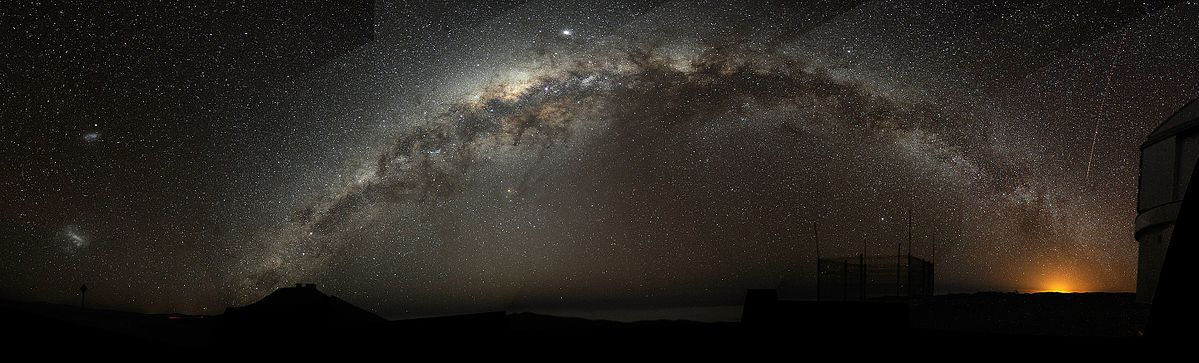
\includegraphics[width=\textwidth]{figures/intro/Milky_Way_Arch}
\caption[~The dust lane of the Milky Way galaxy.]{The Milky Way galaxy, from Cerro Paranal, Chile. The dust, which is mostly confined inside the spiral arms, obscures the glow of billions of background stars. Image from Bruno Gilli/ESO: \url{https://www.eso.org}}
\label{fig:MW}
\end{figure}

It has been almost a century since astronomers first became interested in interstellar dust and began to study its properties in earnest. These earlier astronomers thought of the dust as being somewhat akin to smoke. In \textit{Dust in the Galactic Environment} \citep{whittet2002dust}, the author writes:

\say{The term \textit{smoke} was often used to describe these particles in the early literature. \textit{Smoke} implies the product of combustion, whereas \textit{dust} implies finely powdered matter resulting from the abrasion of solids. The former is arguably more appropriate as a description of the particles condensing in a stellar atmosphere, now regarded as an important source of interstellar grains.}\footnote{Italics added.}

\subsection{Observational Inferences}

Several key observational inferences about the dust point to its role as an important catalyst in both small and large-scale processes related to star formation in galaxies. The grains exhibit differential, or wavelength-dependent extinction, absorbing photons in the optical and near-infrared (O/NIR) while scattering higher energy photons out of the line-of-sight (LOS). The radiation which is absorbed by the grains is re-emitted in the sub-mm/FIR/mm-wave bands. This thermal emission is linearly polarized (see Section~\ref{dust_fields}).

The extinction curve of the interstellar dust indicates a size distribution of $\sim$0.05--0.5~$\upmu$m, where the smallest grains are individual molecules (e.g., polycyclic aromatic hydrocarbons (PAHs)). The exact composition and material properties of the grains are the subject of ongoing study (see, e.g., \citet{andersson2015interstellar,draine2003interstellar}). The O/NIR dust SED indicates that the continuum emission is due to a population of silicate grains, while narrow emission features correspond to PAHs and other carbonaceous grains. The sub-mm/FIR polarization spectrum of the dust, as measured in nearby molecular clouds (MCs), contains a minimum at $\sim$350~$\upmu$m (Figure~\ref{fig:polspec}). This feature indicates that the observed SED is the result of two distinct dust populations.

\begin{figure}[!htbp]
\centering
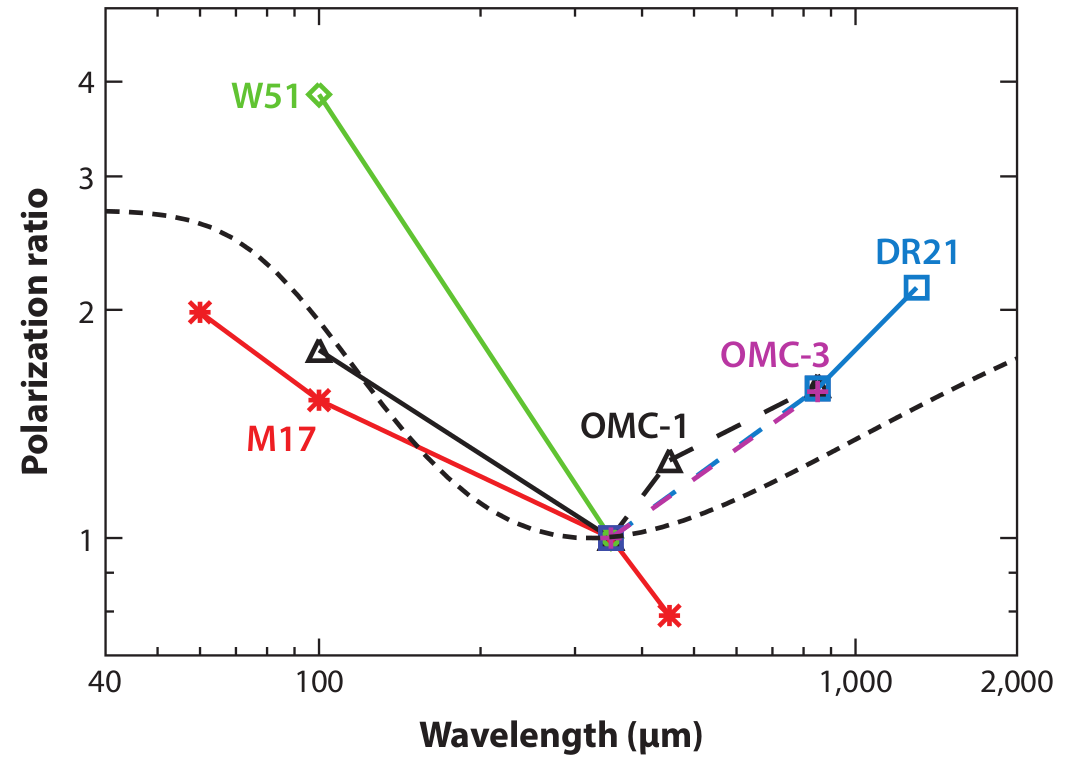
\includegraphics[width=\textwidth]{figures/intro/polspec}
\caption[~The measured polarization spectrum of interstellar dust in several nearby MCs.]{The sub-mm polarization spectrum (normalized to the polarized emission at $\sim$350~$\upmu$m) for several nearby MCs \citep{andersson2015interstellar}. The minimum in the spectrum at $\sim$350~$\upmu$m points to a two-component dust population.}
\label{fig:polspec}
\end{figure}

 Measurements of the spectral energy distribution (SED) of the extragalactic background light (EBL) show that roughly the same amount of energy is contained in the sub-mm/FIR part of the spectrum as in the O/NIR (see Figure~\ref{fig:EBL}). These two distinct regions of the SED are known as the cosmic-optical-background (COB) and cosmic-infrared-background (CIB). The COB and CIB peak at $\sim$1~$\upmu$m and $\sim$100~$\upmu$m. By comparing measurements of the GOODS-S region of the sky taken by BLAST 2006 at 250, 350 and 500~$\upmu$m with those taken in other wavebands, it was discovered that approximately half of the CIB can be associated with individual sub-mm galaxies (SMGs) at cosmological redshifts of $1 \leq z \leq 4$ (\citet{devlin2009over,marsden2009blast,pascale2009blast}). This redshift range corresponds to a period in the universe's history when star formation occurred at rates which are many times higher that which is observed in the present day universe.

\begin{figure}[!htbp]
\centering
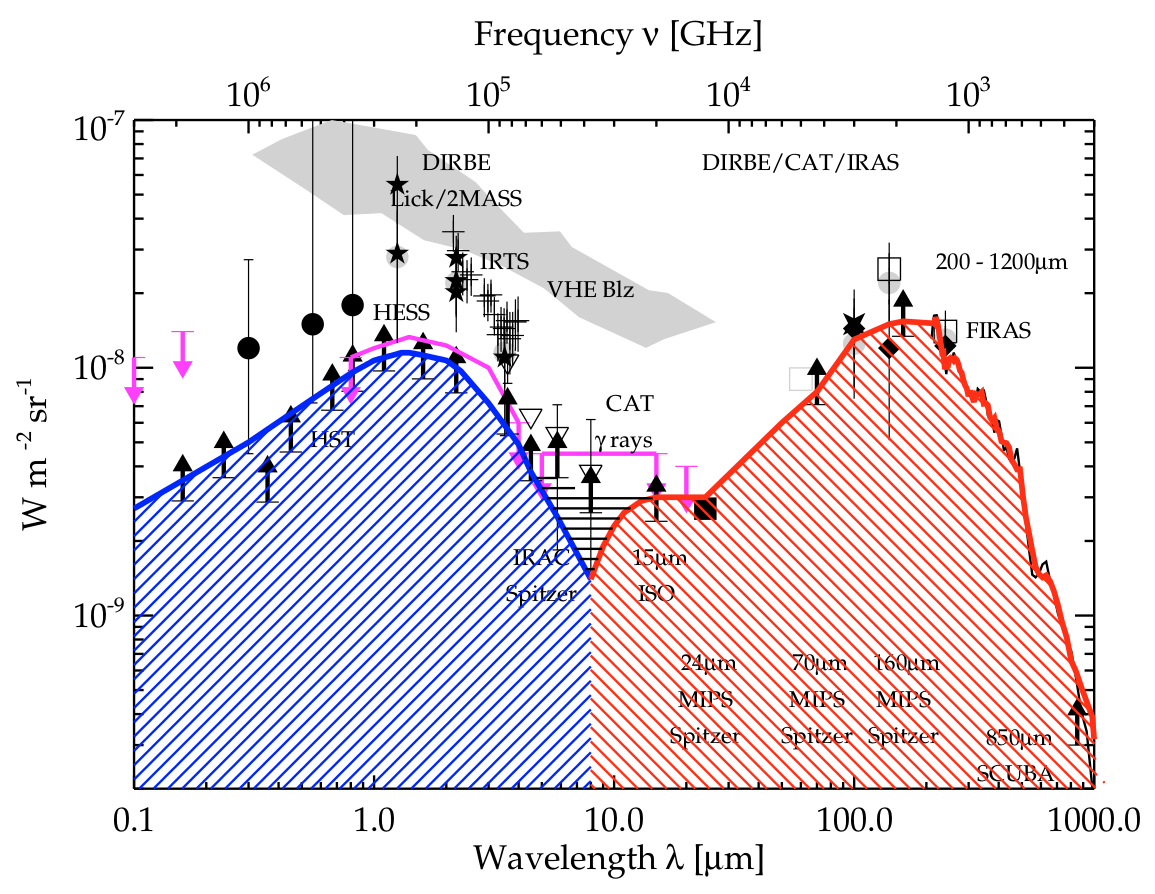
\includegraphics[width=\textwidth]{figures/intro/cob_cib}
\caption[~The SED of extragalactic background light.]{The SED of the EBL, produced from Spitzer observations \citep{dole2006cosmic}. The amount of energy contained in the COB (blue) and CIB (red) is roughly equal.}
\label{fig:EBL}
\end{figure}

\subsection{The Lifecycle of Cosmic Dust}

Interstellar dust is perpetually recycled in the ISM of galaxies. The raw elements of which consists are created by main-sequence stars. These refractory elements condense out of the cool photospheres of AGB stars and planetary nebulae, and form into grains. More dust is created by supernovae.

The dust is dispersed into the ISM surrounding its parent star by stellar winds produced by OB and AGB stars, and by the violent explosions of supernovae. Once in the diffuse ISM, it becomes incorporated into MCs, the birth places of stars. A strong correlation has been observed between the star formation rate (SFR) of galaxies and their dust mass \citep{da2010new}. As a rule of thumb, the gas-to-dust mass ratio of the ISM of the Milky Way and other spiral galaxies is commonly assumed to be $\sim$100.

Inside MCs, The charged surfaces of the grains serve as the sites of molecular hydrogen formation. In the densest regions of MCs, the dust is collisionally coupled to the gas, and shields it from the ionizing radiation from nearby stars. These two effects allow the gas and dust to cool together, and further collapse under gravity. In prestellar cores, the temperatures can range from 10--100~K.

Following star formation, some of the dust grains are recycled by the star, and others become incorporated into newly formed planets. In regions of a galaxy which contain little to no star formation, the remaining dust grains are eventually destroyed by cosmic rays.

\subsection{The Role of Dust as a Tracer of Cosmic Magnetic Fields}\label{dust_fields}

Observed Galactic star formation rates in MCs are far lower than what is expected from a theoretical model of cloud collapse which considers only gravity. Theorists seeking an explanation for what could be slowing the collapse of prestellar cores have settled on two likely culprits. These are supersonic turbulence and magnetic fields (B-fields). Turbulence prevents the effective dissipation of gravitational energy, while B-fields provide an additional source of pressure support that slows, or even halts, the gravitational collapse of MCs.

In the 1930s, astronomers discovered that a small fraction of the O/NIR light which is received from stars is linearly polarized (\citet{hall1949observations,hiltner1949polarization}). The correlation between the polarization of starlight and the previously observed phenomenon of interstellar reddening pointed to cosmic dust as the cause of the polarization. Since the O/NIR starlight is linearly polarized, so is the portion of the starlight which was absorbed by interstellar dust and re-emitted at sub-mm/FIR wavelengths.

The cause of the linear polarization of thermal dust emission is understood as being to due to the aspherical nature of the grains. Through a complex alignment mechanism, the aspherical dust grains, which are spinning due to interactions with the gas and radiation field, end up having their long axes orthogonal to the local B-field direction. Consequently, the electric field (E-field) of the thermal radiation emitted by the dust is preferentially oriented along the long axis of the grains. Therefore, rotating the measured polarization angle of the E-field by 90 degrees yields the direction of the B-field in the plane-of-the-sky (\gls{Bpos}). The strength of the B-field is difficult to estimate. However, indirect methods, such as the Davis-Chandrasekhar-Fermi method (DCFM) \citep{chandrasekhar1953magnetic}, can sometimes be used to place upper constraints on the field strength (see~\ref{carina}).

The physics of the alignment mechanism which is responsible for aligning the dust grains with the local B-field has been the subject of long debate \citep{andersson2015interstellar}. The most commonly accepted mechanism is described by the theory of radiative alignment torques (RAT) \citep{lazarian2007radiative}. In RAT theory, the alignment is facilitated by both the anisotropy of the radiation field and the paramagnetic nature of the dust grains.

\subsection{Combining Total Intensity and Polarization Measurements}

By combining total intensity and polarization measurements of the same region, it is possible to ascertain the relative orientations between \gls{Bpos} and matter structures composed of gas and dust. The data yielded by such observations can be used to model the relationship between the B-field and several environmental variables, including temperature, hydrogen and dust column density and polarization fraction.

The relationship between the above parameters continues to be examined across a wide range of spatial scales.

\begin{comment}
Figure~\ref{fig:vela2006} shows a total intensity map of a region inside the Vela-C MC, taken by BLAST 2006 \citep{netterfield2009blast}. The three colors correspond to the three BLAST bands (blue for 250~$\upmu$, green for 350~$\upmu$, red for 500~$\upmu$), and correspond to different dust temperatures.

\end{comment}

An example of one such analysis is shown in Figure~\ref{fig:vela2012} \citep{fissel2016balloon}. The color scale is the BLASTPol 2012 500~$\upmu$ dust intensity, and the drapery pattern is a line-integral-convolution (LIC) of \gls{Bpos} (see~\ref{LIC}). The spatial resolution in the image is $\sim$2.5~pc, which is sufficient to resolve the large scale filamentary structure of MCs, but not structures within individual filaments (this requires resolution of $\lesssim$0.1~pc).

\begin{comment}
\begin{figure}[!htbp]
\centering
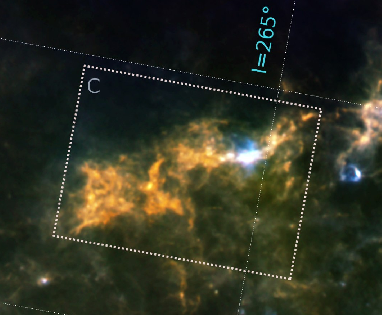
\includegraphics[width=\textwidth]{figures/intro/velac_blast2006_crop}
\caption[~A BLAST 2006 map of Vela C.]{\citet{netterfield2009blast}.}
\label{fig:vela2006}
\end{figure}
\end{comment}

\begin{figure}[!htbp]
\centering
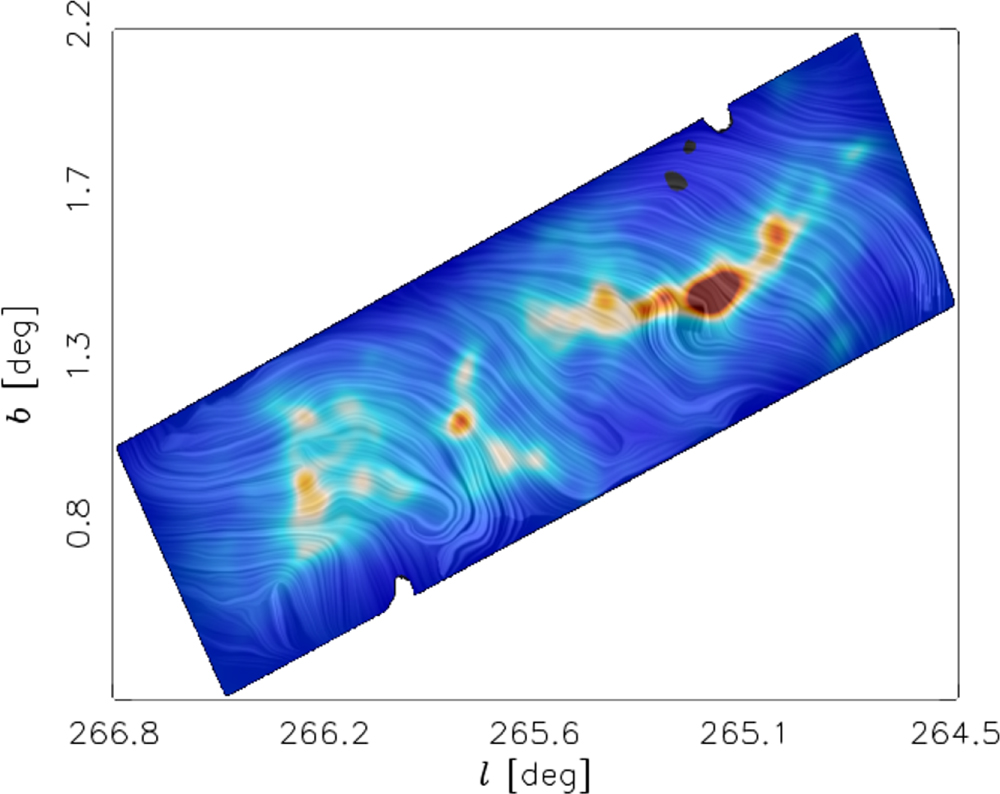
\includegraphics[width=\textwidth]{figures/intro/velac_lic}
\caption[~An LIC map of Vela C, from BLASTPol  2012.]{\citet{fissel2016balloon}.}
\label{fig:vela2012}
\end{figure}

\subsection{The Role of Cosmic Dust as a CMB Foreground}

By virtue of being polarized, thermal emission from interstellar dust grains poses a problem for polarization measurements of the Cosmic Microwave Background (CMB) radiation. It is now known that the polarized emission from diffuse Galactic dust is the dominant CMB foreground at frequencies above 100~GHz \citep{adam2016planck}. Any attempt to detect primordial B-mode polarization in the CMB will be hindered by the dust foreground emission. The solution to this problem is to carefully map the dust polarization in the same regions which are observed by CMB telescopes, over as wide a waveband as possible. The foreground signal can then be cross-correlated with the CMB measurements, and removed.

\section{Technologies for Submillimeter and Millimeter-Wave Astronomy}

Like the charge-coupled device (CCD), the more widespread quantum detector used in astronomical cameras, MKIDs utilize the photoelectric effect. They are incoherent detectors, measuring the total power in the incident electromagnetic radiation (photons), but not the phase. In a semiconductor sensor such as a CCD, the energy band gap of $\sim$1~eV restricts their optical response to between $\sim$0.3--1~$\upmu$m. The superconducting band gap is $\mathcal{O}(10^-3)$ smaller than that of a semiconductor. Consequently, MKIDs (and other superconducting detector technologies) can be engineered to detect radiation spanning the range between mm-waves and Gamma-rays.

The high sensitivity of MKIDs and other superconducting detectors requires that they be operated at a temperature which minimizes their thermal device noise (generation-recombination noise, in an MKID), to below the level of the photon-noise in the passband. As a rule of thumb, this temperature should be $\sim$\gls{Tc}/8 \citep{mazin2013arcons}, where \gls{Tc} is the critical temperature of the device. For a typical MKID \gls{Tc} of $\sim$1.5~K, this corresponds to fridge temperatures of 100--300~mK.

To achieve and maintain such low temperatures throughout an astronomical observation is an engineering feat in its own right. In order to shield the detectors from the thermal radiation of the elements within the optical system, such as mirrors, filters and optomechanics, it is necessary to cool as much of the optical system as possible (sometimes to as low as $\sim$4~K). Cooling of the optics, and detectors (also some of the readout electronics, in certain cases) is facilitated using combinations of open and closed-cycle cryostats which use liquid Helium-4 (LH4) and Helium-3 (LH3) as coolant.

\subsection{KIDs and TESs}

In many aspects, the KID may be considered a successor to the transition-edge sensor (TES) bolometer. TESs, which take a variety forms, have been used by many successful ground, balloon and spaced-based sub-mm/FIR and mm-wave observatories. They are also the chosen sensor technology of several current and planned astronomical observatories (e.g., The Simons Observatory \citep{ade2019simons}).

TESs consist of a superconducting absorber which is part of a voltage-biased circuit that has been tuned to just above the edge of its superconducting transition-edge. The circuit is inductively coupled to a superconducting quantum interference device (SQUID) followed by a low-noise amplifier (LNA). Incident photons cause the absorber to go normal, which increases the resistance of the circuit and leads to a drop in current. The change in current is read out using the SQUID. The voltage-biasing of TESs establishes negative electrothermal feedback, which restores them to their superconducting state after each absorption of a photon.

As astronomical detectors, KIDs and TESs have relative advantages and disadvantages, particularly in regards to their readout systems. A detailed comparison of the two technologies can be found in \citet{mauskopf2018transition}. While more recent TES cameras use FDM readouts ($\upmu$mux, see e.g, \citet{stanchfield2016development}), TESs have been traditionally time-domain multiplexed (TDM). In the TDM readout, $N \times M$ detectors are read out in sequence by $N$-columns of SQUID-switches. In a given data frame, each TES is readout $1/N$ of the time, where $N$ is the multiplexing factor. At present, the highest multiplexing factors which have been achieved are $N$ of 64--128 (\citet{henderson2016advanced,mates2017simultaneous}).

In addition to their limited multiplexing factor, the cryogenic part of the TES readout requires many cryogenic wires/wirebonds ($N + M$ wires for $N \times M$ TESs \citep{mauskopf2018transition}). The thermal noise in the readout chain can be higher than for KIDs, due to the dissipative readout. KIDs, by virtue of being FDM, require only one cryogenic feedline and LNA for $N$ detectors. With the exception of the LNA, their readout electronics are entirely room-temperature.

Despite the relative complexity of their readouts, TESs do have advantages over KIDs. The dissipative readout gives the advantage of self-regulation through electrothermal equilibrium, which increases their response time after each photon hit. KIDs have no equivalent self-regulating mechanism, which makes biasing them somewhat challenging. Another advantage of the TES readout is that the absorbed optical power is is proportional to the readout power dissipated by the bias circuit. With KID readout systems, signal processing must be performed on the raw data outputs in order to make it proportional to the absorbed optical power (see~\ref{blast_data}).

As for their noise properties, TESs are typically stable at frequencies down to a few millihertz. KIDs are observed to have excess noise at low frequencies, which has implications for the mapping capabilities of the experiment (see Section~\ref{flicker noise}).

\section{BLAST-TNG}\label{blast}

\begin{sidewaystable}[!p]
\begin{threeparttable}
\centering
\begin{adjustbox}{width=\textwidth}
\begin{tabular}{@{}lllll@{}}
\dtoprule
 & BLAST (2006) & BLASTPol (2010) & BLASTPol (2012) & BLAST-TNG (2020) \\ \midrule
Bands ($\upmu$m) & 250, 350, 500 & 250, 350, 500 & 250, 350, 500 & 250, 350, 500 \\
Det. type & SiN SWB\tnote{1} & SiN SWB & SiN SWB & LEKID \\
$N_{\mathrm{det}}$ & 149, 88, 43 & 149, 88, 43 & 139, 88, and 43 & $\sim$1500, 700, 300 \\
Pol. & N & Y & Y & Y \\
Aperture (m) & 1.8 & 1.8 & 1.8 & 2.5 \\
Beam FWHM ($\arcsec$) & 36, 42, 60 & $\sim$150\tnote{2} & $\sim$150\tnote{3} & 30, 41, 50 \\
Flight time (days) & 12 & 9 & 13 & 28 (planned) \\ \dbottomrule
\end{tabular}
\end{adjustbox}
\begin{tablenotes}
\item (1) Silicon Nitride (SiN) spider web bolometers (SWB). These were flown on the Herschel Space Observatory's Spectral and Photometric Imaging Receiver (SPIRE) 2009--2013 \citep{griffin2003spire}.
\item (2) A melted IR blocking filter reduced the overall resolution to $\sim$2.5$\arcmin$, after correcting the maps \citep{matthews2014lupus}.
\item (3) The point-spread function (PSF) of the optical beam was warped, resulting in an overall resolution $\sim$2.5$\arcmin$ after correcting the maps \citep{fissel2016balloon}.
\end{tablenotes}
\caption{Comparison of camera parameters between BLAST-TNG, BLASTPol 2012, BLASTPol 2010 and BLAST 2006.}
\label{tab:blast_comp}
\end{threeparttable}
\end{sidewaystable}

The Next Generation Balloon-borne Large Aperture Submillimeter Telescope (BLAST-TNG) is a sub-mm imaging polarimeter which will map the polarized thermal emission from interstellar dust, revealing B-field structures in nearby MCs, giant molecular clouds (GMCs), the diffuse interstellar medium and in nearby external galaxies. It will observe in three bands 30\% bands centered at 250, 350 and 500 microns (1200, 857 and 600 GHz), with spatial resolution of 30$\arcsec$, 41$\arcsec$ and 50$\arcsec$. These physical scales bridge the gap between the 5$\arcmin$ all-sky polarization maps produced by the ESA's Planck space observatory, and ALMA's sub-arcsecond resolution.

The experiment is scheduled for a $\sim$28~day flight from NASA's Long Duration Balloon Facility, near McMurdo Station, Antarctica, in winter 2019/2020\footnote{Several launch attempts were made in winter 2018/2019, but the flight was ultimately delayed until the following season}. BLAST-TNG is the latest incarnation of a series of BLAST experiments which date back to 2005. Previous BLAST payloads had successful flights in 2005, 2006, 2010 and 2012. Table~\ref{tab:blast_comp}list key instrumental parameters for each of these experiments. BLAST-TNG is `next-generation' for several reasons. Chief among these are:

\vspace{5mm}

\textit{Detectors and readout electronics}: BLAST-TNG is the first NASA-funded balloon experiment to feature large-format (kilo-pixel scale) arrays of LEKIDs, along with the highly multiplexed FPGA-based electronics which are required to read them out\footnote{In summer, 2018, the ASI's OLIMPO balloon succeeded in being the first flight for LEKID detectors. Their readout system was based on the firmware and software from the ASU detector system, with a modified set of intermediate frequency (IF) electronics (see Section~\ref{kid cameras})}. Its camera features $\sim$3,000 dual-polarization sensitive, horn-coupled LEKIDs, which are fabricated from trilayer substrate consisting of a titanium nitride/titanium/titanium nitride (TiN/Ti/TiN) \citep{hubmayr2014dual}. In this capacity, BLAST-TNG serves as a pathfinder for upcoming balloon experiments, including EXCLAIM \citep{switzer2017measuring} and TIM/STARFIRE \citep{aguirre2018starfire}.

\vspace{5mm}

\textit{Primary mirror}: BLAST-TNG's 2.5~m diameter primary mirror is based on a composite carbon fiber reinforced polymer (CFRP) design developed by Alliance Spacesystems\footnote{\url{https://alliancespacesystems.com/}}. The primary mirror will be the largest to-date which has flown on a long-duration stratospheric balloon.The optical design of BLAST-TNG is described in \citet{lourie2018design}.

\vspace{5mm}

\textit{Mapping speed}: With its large aperture primary mirror and over $\sim$2,500 LEKID detectors, BLAST-TNG is expected to have $\sim$6 times the mapping speed of its predecessor, BLASTPol 2012. The resulting maps will contain hundreds of thousands of B-field pseudo-vectors-- an order of magnitude improvement over BLASTPol.

\subsection{Science with BLAST-TNG}

BLAST-TNG will perform five science surveys, covering the following categories:

\vspace{5mm}

\textit{Nearby Molecular Clouds}: These are the closest sites of active star formation (visible from McMurdo Station, Antarctica). BLAST-TNG will map B-fields down to the scale of filaments of gas and dust which thread MCs. Many of the dense cores which form the nodes of these filaments will form into stars. These maps will enable the study of correlations between physical and environmental parameters in the MC, including the dust polarization fraction and spectrum, gas and dust temperatures, column densities, and B-field direction and strength (see, e.g., \citet{galitzki2014balloon,fissel2016balloon,fissel2018relative,shariff2019submillimeter,gandilo2016submillimeter}).

\vspace{5mm}

\textit{Giant Molecular Clouds}: GMCs are among the densest regions of the ISM, and host large amounts of massive star formation. The clusters of massive O and B stars which form inside GMCs inject energy into the surrounding ISM via ionizing radiation, stellar winds and supernovae.
\vspace{5mm}

\textit{Diffuse Galatic ISM}: In order to constrain physical models of different dust populations and their alignment mechanisms, it is necessary to probe structures within the ISM across a wide range of densities. This includes mapping the lower density, diffuse regions of the ISM. These observations will provide input to numerical models which test the correlation between the measured dust polarization properties and the orientation of the B-field.

\vspace{5mm}

\textit{CMB Foregrounds}: Mm-wave measurements of polarization in the CMB are contaminated by the polarized dust emission. High resolution maps of the polarized dust emission in the regions observed by CMB observatories are required to clean the CMB maps of this foreground. Around 100 hours of the BLAST-TNG flight is designated to mapping polarized dust emission on degree scales in regions of the sky that overlap with those previously mapped by CMB observatories.

\vspace{5mm}

\textit{Nearby External Galaxies} B-fields constitute a significant part of the energy density in galactic ISMs. Through flux freezing and channeling of cosmic ray electrons, they can influence the evolution of structure over a wide range of physical scales within a galaxy. At radio wavelengths, synchrotron emission and Faraday rotation has been used to map the large scale fields in a variety of galaxy types, including spirals, ellipticals, dwarf irregulars and interacting pairs. BLAST-TNG will complement these radio observations with the first comprehensive survey of \gls{Bpos} as traced by interstellar dust (see~\ref{target selection}).

\section{Current KID-based Instruments}\label{kid cameras}

BLAST-TNG and the ASU LEKID readout build on the legacy of past sub-mm/mm-wave cameras (e.g. MUSIC \citep{golwala2012status} and MAKO \citep{swenson2012mako}), as well as MKID-based O/NIR cameras (e.g., ARCONS \citep{mazin2013arcons}, DARKNESS \citep{meeker2018darkness,strader2016digitial}). While much of the electronics, firmware and software which is required to readout MKIDs is similar for sub-mm/mm-wave and O/NIR cameras, the mode in which the detectors are operated is different.

\subsection{Considerations on Sub-mm/mm-wave and O/NIR MKID Readout Systems}

In the sub-mm/mm-wave, MKIDs are used in bolometer-mode, as power detectors. In the O/NIR, they are used in Geiger-mode, to count single photon arrival times and measure their energy. When KIDs are operated in bolometer (or background-limited infrared photon, BLIP) mode, slow variations in the background loading cause them to drift off-resonance. To track the detectors' responsivities during an observation requires `tuning' the probe tones which are generated by the readout system in amplitude and frequency. Tuning can be implemented in either firmware or software, and depending on the number of detectors and detector parameters which are taken into account, can be very resource and time intensive (see, e.g. \citet{dodkins2018mkid}).

While sub-mm/mm-wave MKID systems must address the tuning requirement, they have the advantage of being able to readout data at lower-rates than O/NIR systems, which must be able to register the arrival times of individual photons.

\subsection{KID Instruments which Incorporate Elements of the ASU LEKID Readout}

At the time of writing, the ASU LEKID readout is a core system of several current and planned sub-mm/mm-wave instruments. Because each instrument has different system requires, the elements of the readout (IF electronics, firmware, software) are used to varying extents in each system. Key instrumental parameters for each camera are listed in in Table~\ref{tab:cameras}, and the instruments are summarized below.

\begin{sidewaystable}[!p]
\begin{threeparttable}
\centering
\begin{adjustbox}{width=\textwidth}
\begin{tabular}{@{}llllll@{}}
\dtoprule
 & TolTEC & BLAST-TNG & MUSCAT & OLIMPO & SuperSpec \\ \midrule
N$_{\mathrm{Det.}}$ & 900, 1800, 3600 & 300, 700, 1500 & 1600 & 19, 37, 23, 41 & 300 \\
N$_{\mathrm{R2}}$ & 13 & 5 & 4 & 2 & 1 \\
$f_{\mathrm{res}}$ (MHz) & $\sim$500--1000 & $\sim$500--1000 & $\sim$500--1000 & $\sim$0--150 & $\sim$100--600 \\
Bands (GHz) & 150, 214.14, 272.5 & 600, 856, 1200 & 272.5 & 150, 250, 350, 460 & 185--315 \\
Bands (mm) & 2, 1.4, 1.1 & 0.500, 0.350, 0.250 & 1.1 & 2, 1.2, 0.86, 0.67 & 1.62--0.95 \\
Mode\tnote{1} & BP & BP & BP & SP & SP \\
Couplng\tnote{2} & HC & HC & HC & HC & AC \\
Material & TiN/Ti/TiN & TiN/Ti/TiN & Al & Al & TiN \\
\gls{Tbase} (mK) & 0.1 & 0.28 & 0.1 & 0.3 & 0.25 \\
Site & LMT & LDB & LMT & LMT & Svalbard \\
Altitute (km) & 4.6 & $\sim$35 & 4.6 & $\sim$38 & 4.6 \\
Aperture (m) & 50 & 2.5 & 50 & 2.6 & 50 \\
Beam FWHM ($\arcsec$) & 9.5, 6.3, 5 & 50, 41, 30 & 5.5 & 194, 116, 83, 63 & NA \\
R ($\lambda/\Delta \lambda$) & NA & NA & NA & $\sim$100 & $\sim$300 \\
Platform & Ground & Balloon & Ground & Balloon & Ground \\
\begin{tabular}[c]{@{}l@{}}Total NEP W/$\sqrt{\mathrm{Hz}}$\\ $\times$ 10$^{-17}$\end{tabular} & $\sim$1\tnote{a} & $\sim$5\tnote{b} & $\sim$1\tnote{c} & $\sim$1\tnote{d} & $\sim$0.3--0.4\tnote{e} \\  \dbottomrule
\end{tabular}
\end{adjustbox}
\begin{tablenotes}
\item (1) Horn coupled (HC) or antenna coupled (AC).
\item (2) Bolometric polarimetry (BP) or spectro-photometry (SP).
\item (a) \url{http://toltec.astro.umass.edu/about}
\item (b) See~\ref{blast_data}.
\item (c) Assuming comparable to TolTEC.
\item (d) \citet{paiella2019kinetic}
\item (e) \citet{mcgeehan2018low}
\end{tablenotes}
\caption{Camera parameters for systems currently using elements of the ASU LEKID readout.}
\label{tab:cameras}
\end{threeparttable}
\end{sidewaystable}

\vspace{5mm}

\textit{OLIMPO}: OLIMPO (\citet{masi2008olimpo,paiella2019kinetic}) is a large aperture (2.6~m) balloon–borne mm-wave telescope which is designed to measure the Sunyaev-Zeldovich effect (SZ). It has four bands, centered at 150, 250, 350, and 460~GHz (2, 1.2, 0.86, 0.67~mm), which utilize 19, 37, 23 and 41 aluminum (Al) horn-coupled LEKIDs. The instrument performs spectrophotometry using a differential Fourier transform spectrometer (DFTS) which can be inserted into the optical path using a movable relay mirror.

In summer, 2018, OLIMPO had a successful flight from Svalbard, Norway. This was the first flight for KID detectors and their associated FPGA-based readout electronics. The camera incorporated the ASU ROACH2 electronics, firmware and software (two ROACH2 slices). In addition to the milestone which it represents for this detector technology, the data which was obtained during the flight regarding the performance of both the detectors and the readout system is invaluable to upcoming KID-based balloon-borne cameras (including BLAST-TNG).

An analysis of the camera's in-flight performance is presented in \citet{masi2019kinetic}. The analysis examines the detector and readout system's noise performance, response to cosmic ray hits, and thermal behavior during the flight. It determined that in all categories, the camera performed as expected-- a finding that bodes very well for future KID cameras.

Figure~\ref{fig:olimpo cal lamp}~\citep{masi2019kinetic} shows a detector phase timestream containing a calibration lamp (cal lamp) chop (left) and detector noise PSDs (right) for the same channel, taken on the ground (red) and during the flight (blue). The cal lamp chop is a diagnostic used to measure the detector responsivities. The noise is lower in-flight by a factor of $\sim$2.5, due to the decreased thermal loading on the detectors from the colder environment at float altitude ($\sim$38~km).

\begin{figure}[!htbp]
\centering
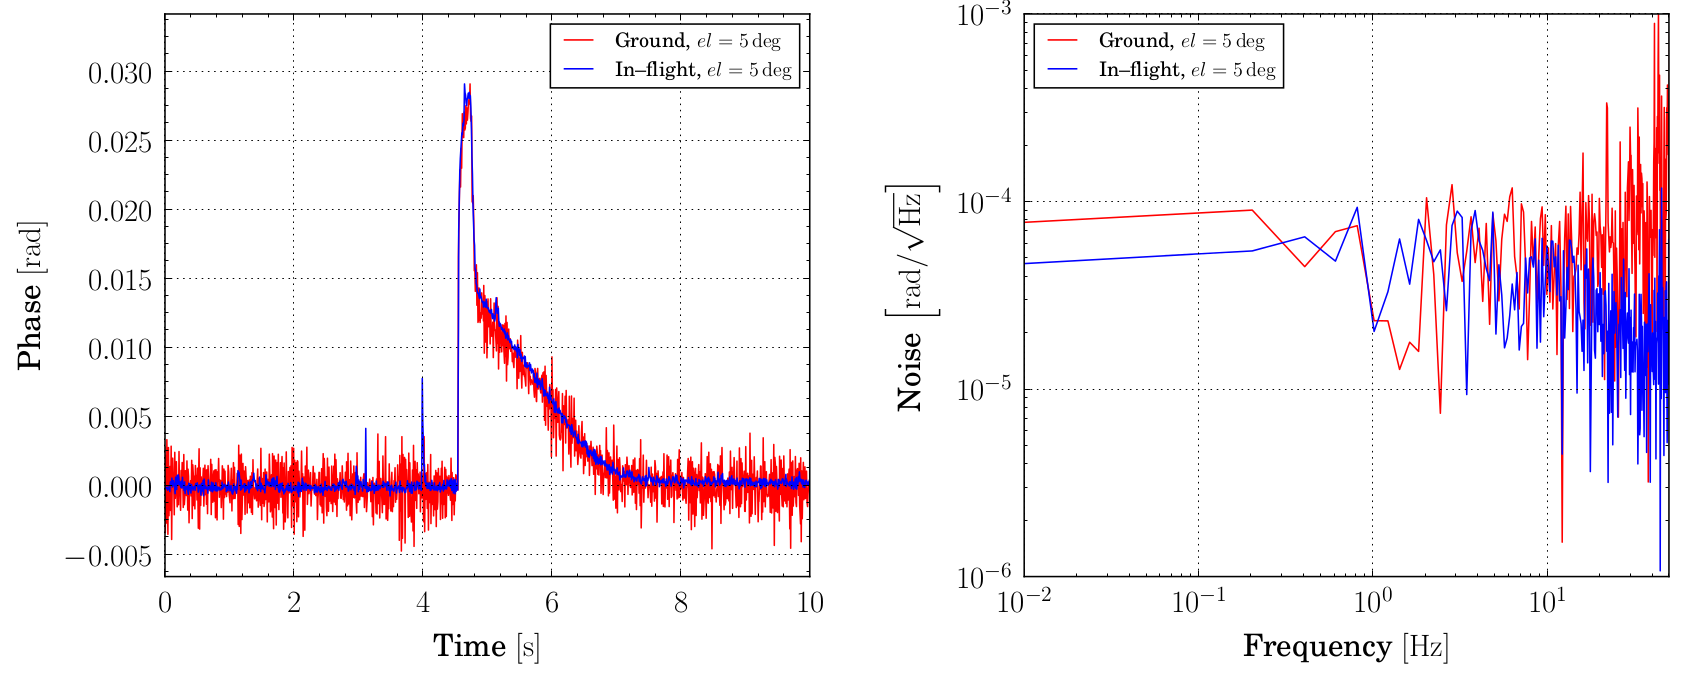
\includegraphics[width=\textwidth]{figures/intro/olimpo_cal_lamp}
\caption[~A cal lamp chop and PSD from the 2018 OLIMPO balloon flight.]{Data from a single detector taken during the 2018 OLIMPO balloon flight. The left frame shows the timestream of a cal lamp chop, taken on the ground (red) and in flight (blue). The right frame is the noise PSD for the same channel, on the ground (red) and in-flight (blue). The noise is lower in-flight by a factor of $\sim$2.5, due to lower thermal loading on the detectors. Image is from \citet{masi2019kinetic}.}
\label{fig:olimpo cal lamp}
\end{figure}

\vspace{5mm}

\textit{TolTEC}: TolTEC \citep{toltec} is a mm-wave camera which will be a facility instrument on the LMT, with first-light planned for 2019. Its camera is based on $\sim$7,000 dual-polarization sensitive trilayer TiN/Ti/TiN horn-coupled LEKIDs, similar to those used in BLAST-TNG, distributed between three bands centered at 2, 1.4, and 1.11~mm (50, 220, and 280~GHz) \citep{austermann2018millimeter}. The readout uses the ROACH2 firmware, software and IF electronics which have been developed for BLAST-TNG ($\sim$13 readout slices, versus the 5 used for BLAST-TNG). When coupled to the 50~m aperture of the LMT, TolTEC will have unprecedented spatial resolution in the mm-wave band (9.5$\arcsec$, 6.3$\arcsec$ and 5$\arcsec$). This will enable it to produce several unique data sets.

Soon after first-light, the TolTEC collaboration will conduct Four Public Legacy Surveys which will be made freely accessible to the public after $\sim$1--2~years. Some of first science surveys that are planned for TolTEC include\footnote{\url{http://toltec.astro.umass.edu/science}}:

\begin{itemize}[nosep]
  \item 100~deg$^{2}$ Large Scale Structure Survey
  \item 1~deg$^{2}$ confusion limited Ultra-Deep Galaxy Survey
  \item 90~deg$^{2}$ Clouds-to-Cores Legacy Survey
  \item Legacy Surveys of Nearby Galaxies
  \item The Cluster Cosmology Survey
  \item Magnetic Fields and Star Formation
  \item The Interrogation of Comets
\end{itemize}

\vspace{5mm}

\textit{Mexico-UK Submillimeter Camera for Astronomy (MUSCAT)}: MUSCAT \cite{brien2018muscat} is a LEKID camera which will be installed at the LMT along with TolTEC. It is based on four sub-arrays of horn-coupled LEKIDs (1,600 in total) which are cooled to 100~mK, and will observe in a single band centered at 1.1~mm. MUSCAT utilizes the BLAST-TNG ROACH2 firmware and IF electronics.

\vspace{5mm}

\textit{SuperSpec}: SuperSpec (\citet{superspec};\citet{wheeler2018superspec}) is an on-chip filter-bank spectrometer based on antenna-coupled TiN KIDs which will have its first on-sky engineering run at the LMT in 2019. It will perform moderate resolution (R $\sim$ 300) spectroscopy over 190--310 GHz (1.57--0.98~mm) using 300 channels. SuperSpec will measure redshifted line emission (e.g., [CII]) in submillimeter galaxies (SMGs) at cosmological redshift $z$ of 5--9, as well as CO emission in galaxies at lower $z$.

The SuperSpec camera incorporates the ROACH2 electronics, firmware and software developed for the BLAST-TNG readout. Figure~\ref{fig:readout noise comp} \citep{mcgeehan2018low} shows a comparison between the fractional frequency noise \gls{Sxx} of the system measured at a base temperature of 210~mK using the SuperSpec ROACH2 system and a Vector Network Analyzer (VNA) for tone combs consisting of 1 (blue and green) and 50 (red and pink) channels. The noise power spectral densities (PSDs) are shown for timestreams which correspond to the on and off-resonance states (see Chapter~\ref{blast_data}). Horizontal lines represent the expected photon-noise at the LMT sight. The system noise (including the LNA, readout, and detectors) which is measured with the ROACH2 system is comparable to that which is measured using VNA, for both the single and multitone combs.

\begin{figure}[!htbp]
\centering
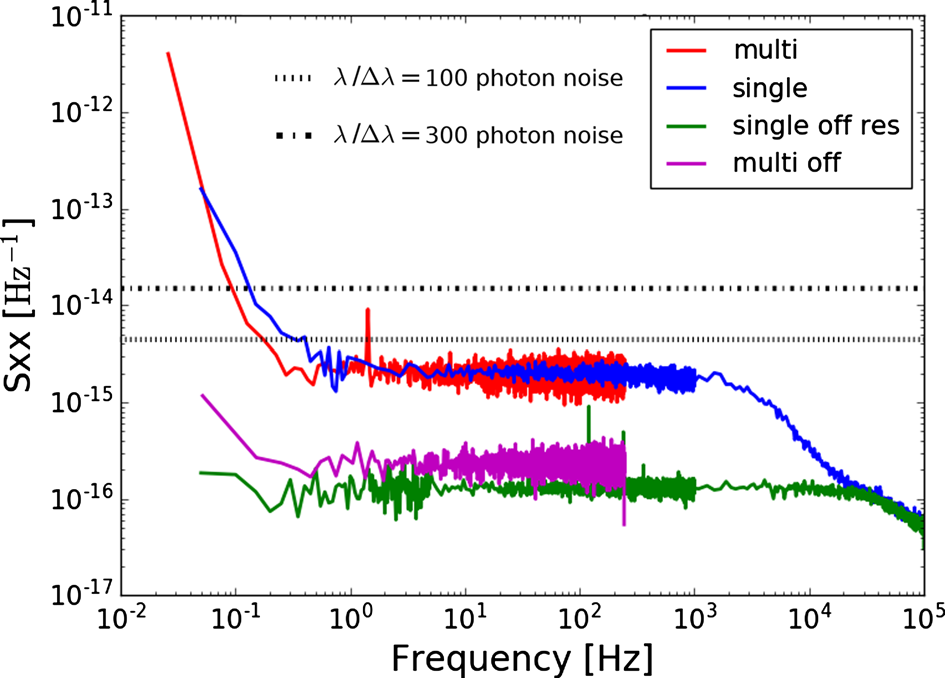
\includegraphics[width=\textwidth]{figures/intro/superspec_noisecomp}
\caption[~Comparison of the fractional frequency noise measured using the SuperSpec ROACH2 system and a VNA for single and multitone combs.]{A comparison of the fractional frequency noise \gls{Sxx} measured using the SuperSpec ROACH2 system and a VNA for single and multitone combs. The horizontal lines represent the expected photon-noise at the LMT sight. The ROACH2 system noise is comparable to that of the VNA, for both the single and multitone combs. Image taken from \citet{mcgeehan2018low}.}
\label{fig:readout noise comp}
\end{figure}

\vspace{5mm}

\textit{Future Instruments}: In addition to the experiments listed above, two recently funded balloon-borne cameras will incorporate elements of the ASU LEKID readout, with added improvements to the firmware and electronics which are made possible by the advent of ultra-high bandwidth FPGA boards (see~\ref{conclusion}). These are: The Experiment for Cryogenic Large-aperture Intensity Mapping (EXCLAIM) \citep{switzer2017measuring}, and the Terahertz Imager (TIM/STARFIRE) \citep{aguirre2018starfire}.

\section{Dissertation Outline}

This dissertation is organized as follows:

\begin{itemize}
\item Chapter~\ref{kid_model} describes a parametric model of a LEKID which can be used to simulate the behavior of both dark and optically loaded pixels, as well as to fit measurements of actual LEKIDs.

\item Chapter~\ref{readout} introduces the ASU LEKID readout, and details the system requirements, the architecture of the firmware, software and electronics, and the verification of the DSP pipeline and noise performance.

\item Chapter~\ref{blast_data} describes the instrumental characterization of the BLAST-TNG receiver and detector arrays which was conducted during the instrument integration at NASA's Columbia Scientific Balloon Facility (CSBF) in summer, 2018, as well as during pre-flight testing at NASA's Long Duration Balloon site (LDB) near McMurdo Station, Antarctica, during November through January, 2018/2019. The parametric LEKID model presented in Chapter~\ref{kid_model} is applied to measured detector data in order to understand various characteristics of the detector arrays and the instrument as a whole.

\item Chapter~\ref{carina} presents an original data analysis of the B-field morphology in the Carina Nebula Complex (CNC, NGC 3372), using a map of the region taken during the BLASTPol 2012 flight. In that analysis, we present what are possibly the first estimates of the strength of \gls{Bpos} over the inner $\sim$1.25~deg$^{2}$ of the CNC.

\item Chapter~\ref{galaxies} presents a target selection survey of five nearby external galaxies which will be mapped during the 2019/2020 BLAST-TNG flight.

\item Chapter~\ref{mcp} contains an operator's manual for the $C$-based BLAST-TNG detector readout flight software, which includes a description of the in-flight detector readout strategy.

\item Chapter~\ref{conclusion} presents conclusions, with a discussion of how the technological landscape has evolved since this work began, and how it can benefit from recent developments in the area of high speed DSP.

\end{itemize}

\chapter{Parametric model of a LEKID}\label{kid_model}

In the following, we develop a parametric model of a kinetic inductance detector (KID) which can be used to interpret or fit actual measurements produced by KID cameras or experiments. The model simulates both intrinsic circuit parameters and measured experimental values as a functions of base temperature \gls{Tc} and absorbed optical power \gls{Pabs}. To be able to make accurate predictions, the model must incorporate the underlying device physics of KIDs. These physics are described within the framework of superconductivity.

The KID model contains several device properties which require initial values. These parameters, and the initial values which were used to produce the figures presented in the following sections, are listed in Table~\ref{table:kid sim}. The definition of each parameter can be found in the glossary section at the beginning of this document, or in the text below.

This chapter is organized as follows:

\begin{itemize}[nosep]
  \item Section~\ref{sec:supercond} provides a brief overview of relevant concepts from superconductivity.
  \item Section~\ref{sec:kinetic_inductance} introduces the kinetic inductance (KI).
  \item Section~\ref{sec:kid_params} describes the temperature and power dependence of key instrinsic and empirically determined values.
  \item Section~\ref{sec:responsivity} defines the KID responsivity to changes in \gls{Tc} (\gls{Rtemp}) and \gls{Pabs} (\gls{Ropt}).
  \item Section~\ref{sec:sensitivity} defines the instrumental sensitivity, and describes the instrumental noise budget for a KID instrument, detailing how each of the dominant noise sources contributes to the total noise-equivalent power (NEP).
\end{itemize}

\begin{table}[!htbp]
\centering
\begin{tabular}{@{}llll@{}}
\dtoprule
Parameter                         & 250~$\upmu$m         & 350~$\upmu$m         & 500~$\upmu$m         \\ \midrule
$w_{\mathrm{L}}$ ($\upmu$m)                  & 8                  & 10                 & 4                  \\
$l_{\mathrm{L}}$ ($\upmu$m)                  & 600                & 900                & 670                \\
$t_{\mathrm{L}}$ ($\upmu$m)                  & 18                 & 18                 & 20                 \\
\gls{N0} (ev$^{-1}$$\upmu$m$^{-3}$)     & 9.8 $\times 10^{10}$ & 9.5 $\times 10^{10}$ & 3 $\times 10^{10}$ \\
\gls{Tc} (K)                         & 1.46               & 1.55               & 1.30               \\
$\tau_{\mathrm{rec},0}$ (s)                    & 3 $\times 10^{-6}$ & 3 $\times 10^{-6}$ & 3 $\times 10^{-6}$ \\
$T_{\mathrm{LNA}}$ (K)            & 6                  & 6                  & 6                  \\
$Q_{loss}$                        & 10$^{7}$           & 10$^{7}$           & 10$^{7}$           \\
\gls{Qc}                           & 4 $\times 10^{4}$  & 4 $\times 10^{4}$  & 4 $\times 10^{4}$  \\
\gls{sig_n} ($\Omega$ cm)$^{-1}$ & 7000               & 7000               & 7000               \\
\gls{Tbase} (mK)          & 290                & 290                & 290                \\
\gls{Popt} (dBm)          & -90                & -90                & -90                \\
\gls{opt_eff}                     & 1                  & 1                  & 1                \\
\gls{det_eff}                     & 1                  & 1                  & 1                \\
\dbottomrule
\\
\end{tabular}
\centering
\caption[~Initial values of device parameters used in the KID model.]{Initial values of device parameters used in the KID model.}
\label{table:kid sim}
\end{table}

\section{Cooper Pairs and Quasiparticles}\label{sec:supercond}

A superconductor is a conductor whose DC resistance $R$ disappears when it is cooled below a material-specific temperature known as the critical temperature \gls{Tc}. The disappearance of $R$ is accompanied by the expulsion of magnetic field (B-field) lines from inside the material, which increases the magnetic flux at surface. The latter phenomenon is known as the Meissner effect.

That $R$ goes to zero when a superconductor is cooled below \gls{Tc} implies (by Ohm's Law) that an infinite DC current can be generated by the application of a finite voltage. However, superconductors have non-zero impedance, because the reactance (capactive and inductive) does not disappear along with $R$. The inductance of the superconductor prevents the instantaneous formation of current. Past a maximum current known as the critical current \gls{Ic}, the superconductor reverts to its normal state. Similarly, the superconductivity can be destroyed by applying a an external B-field whose strength exceeds the material's critical field $B_{c}$.

The underlying physics of superconductivity was first described by Bardeen-Cooper-Schrieffer (BCS) theory \citep{bardeen1957theory}. In BCS, when a superconductor is cooled below \gls{Tc} a supercurrent is created that consists of paired normal charge carriers (holes and electrons) called Cooper pairs (CPs). The remaining charge carriers which have not formed pairs are referred to as quasiparticles (QP). QP have the same spin and charge as normal electrons, but have an effective mass \gls{mstar} which differs from the rest mass of an electron \gls{m_e}.

CPs are modeled as quasi-bosons with mass of $2\gls{m_e}$ and charge of $2e$. The pairs arise from electron-phonon interactions in the crystal lattice of the conductor. Cooling the material decreases the thermal vibrations in the cation lattice. A single QP moving through the lattice attracts several cations, creating a local overdensity of positive charge, or a phonon, which propagates along with the QP. A second QP, having opposite spin to the first, becomes attracted to the phonon, forming the second member of the CP. The pairs have coherence lengths which are typically several orders of magnitude greater than the lattice spacing.

From an energy standpoint, the formation of supercurrent is the consequence of the creation of an energy band gap which forms above and below the material's Fermi energy:

\begin{equation}\label{eq:bandgap}
  E_{g}(T = 0) = \gls{Delta} = \frac{3.52}{2}k\gls{Tc}
\end{equation}

where $k$ is Boltzmann's constant, and \gls{Delta} is the value of the band gap at absolute-zero. The Fermi energy, $E_{F}$, is the difference in the energy between the highest and lowest states which are occupied by the fermions (electrons and holes) at $T = 0$~K \citep{kittel1998thermal}:

\begin{equation}\label{eq:Fermi_energy}
  E_{F} = \frac{\hbar^{2}}{2 \gls{mstar}}\left( \frac{3 \pi^{2} \gls{N0}}{\Sigma} \right)
\end{equation}

where $\Sigma$ is the volume of the conductor, and \gls{N0} is the single-spin density of states at the Fermi energy. During cooling, the rate of the decline in $R$ with $T$ is material dependent. For example, the decline is much faster in aluminum (Al) devices than in titanium nitride (TiN) devices \citep{mauskopf2018transition}. The band gap energy \gls{Delta} is equivalent to the CP binding energy, and is typically of $\mathcal{O}(10^{-3})$~eV. This band gap is around three orders of magnitude smaller than that of semiconductors, including CCDs, which illustrates the potential sensitivity advantages of using superconductors as detectors.

Any energy greater than $2\gls{Delta}$ which is absorbed by a superconductor will unbind, or break apart a CP into its constituent QP. This breaking apart of CPs can be measured to estimate the total power which is absorbed by a device. In the case of a KID, the splitting of CPs is measured by proxy, using the corresponding change in KI (see Section~\ref{sec:kinetic_inductance}). In Section~\ref{QP} we will derive an equation which contains the band gap energy's dependence on \gls{Tc} and \gls{Pabs}.

\subsection{Quasiparticle Generation and Recombination}\label{QP}

In a KID, QP are generated and recombine (CPs dissociate and reform) due to the absorption of thermally generated phonons in the material. These phonons may be produced by temperature fluctuations in \gls{Tbase}, or from power dissipated by the microwave carrier tone which is used to readout the device. QP are also generated by the absorption of photons with frequency $\nu \geq 2\gls{Delta}/h$. In the superconducting materials used to fabricate sub-mm/mm-wave KID devices, typical QP lifetimes (recombination times) \gls{tau_qp}, are $\mathcal{O}$(10)~$\upmu$s. An empirical expression for the QP lifetime which has been found to apply to several materials is \citep{zmuidzinas2012superconducting}:

\begin{equation}\label{eq:tau_qp}
  \gls{tau_qp} = \frac{\tau_{max}}{1 + \gls{nqp}(T)/n^{\star}}
\end{equation}

where $\gls{nqp}(T)$ is the number density of thermally generated QP, and $n^{\star}$ $\sim$ 100~$\upmu$s is the cross-over number density. The QP which are generated by thermal phonon absorption and by pair-breaking photons can be modeled as two distinct populations.

The total number density of QP is \citep{mauskopf2018transition}:

\begin{equation}\label{eq:nqp_tot}
  \begin{aligned}
  n_{qp,\mathrm{tot}} &= \gls{nqp}(T) + \gls{nqp}(P) \\
          &= 4\gls{N0} \int_{0}^{\infty} \frac{dE}{1 + e^{E/k\gls{Tc}}} \\
          &= 4N_{0}k\gls{Tc}\text{ln(2)}
  \end{aligned}
\end{equation}

Io separate out the effects of varying \gls{Tbase} and \gls{Pabs}, the thermal and optical QP number densities must be written explicitly. In the low temperature limit ($T \ll \gls{Tc}$) the number density of thermal QP is

% QP number density
\begin{equation}\label{eq:Nqp_T}
  \begin{aligned}
  \gls{nqp}(T) &\simeq 2\gls{N0}\sqrt{2\pi k T \gls{Delta}}e^{-\gls{Delta}/kT} \\
               &= \frac{\gls{Nqp}(T)}{\Sigma}
  \end{aligned}
\end{equation}

\begin{comment}
\begin{equation}\label{eq:density of states}
   \gls{N0} = \frac{\Sigma}{3\pi^{2}} \left( \frac{2 E_{F} \gls{mstar}} { \hbar^{2} } \right)^{3/2}
\end{equation}
\end{comment}

where $\Sigma$ is the volume of the inductor, and $\gls{Nqp}(T)$ is the total number of thermally generated QP. Figure~\ref{fig:Nqp_T} shows $\gls{Nqp}(T)$ for a range of base temperatures.

The number of QP produced per absorbed photon of frequency $\nu$ can be found by taking the ratio of the photon energy to the band gap energy:

% number of QP per photon
\begin{equation}\label{eq:qp_per_photon}
  \gls{Nqp}(\nu)_{\mathrm{,per}} = \frac{\gls{det_eff} h\nu}{\gls{Delta}}
\end{equation}

where \gls{det_eff} is the detector quantum efficiency (typically $\sim$80\%). The number of broken CPs per absorbed photon would be half of Equation~\ref{eq:qp_per_photon}. The corresponding number of optically generated QP is:

% number of optically generated QP
\begin{equation}\label{eq:Nqp_P}
  \begin{aligned}
  \gls{Nqp}(P) &= \frac{ \gls{det_eff}\gls{opt_eff} \gls{Nqp}(\nu)_{\mathrm{,per}} \gls{Pabs}\gls{tau_qp}}{h\nu} \\
              &= \frac{\gls{Nqp}(\nu)_{\mathrm{,per}}\gls{Popt}\gls{tau_qp}}{h\nu}
  \end{aligned}
\end{equation}

\begin{figure}[!htbp]
\centering
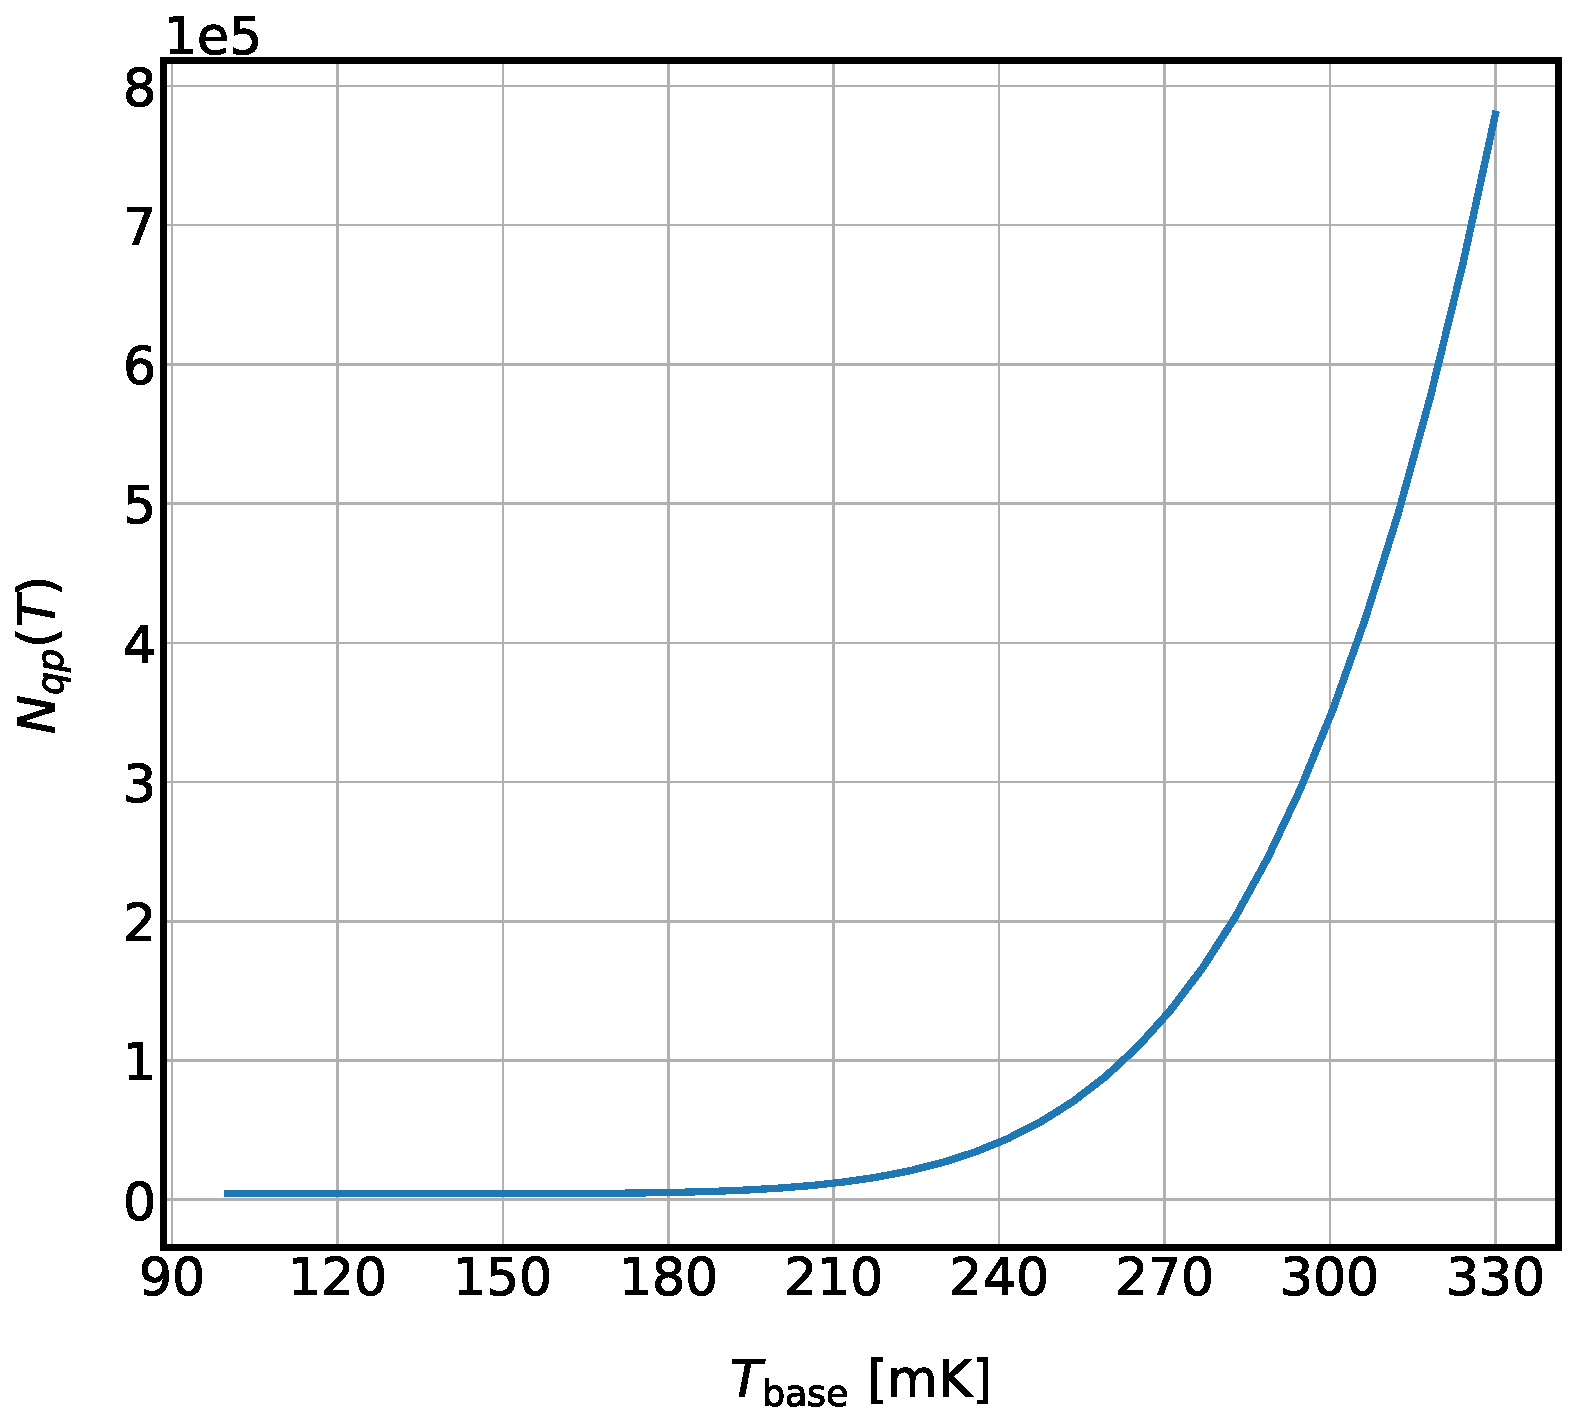
\includegraphics[width=0.8\textwidth]{figures/kid_model/Nqp_T}
\caption[~\macrocapwrap{\gls{Nqp}} as a function of base temperature.]{The total number of thermally generated QP as a function of base temperature.}
\label{fig:Nqp_T}
\end{figure}

\begin{figure}[!htbp]
\centering
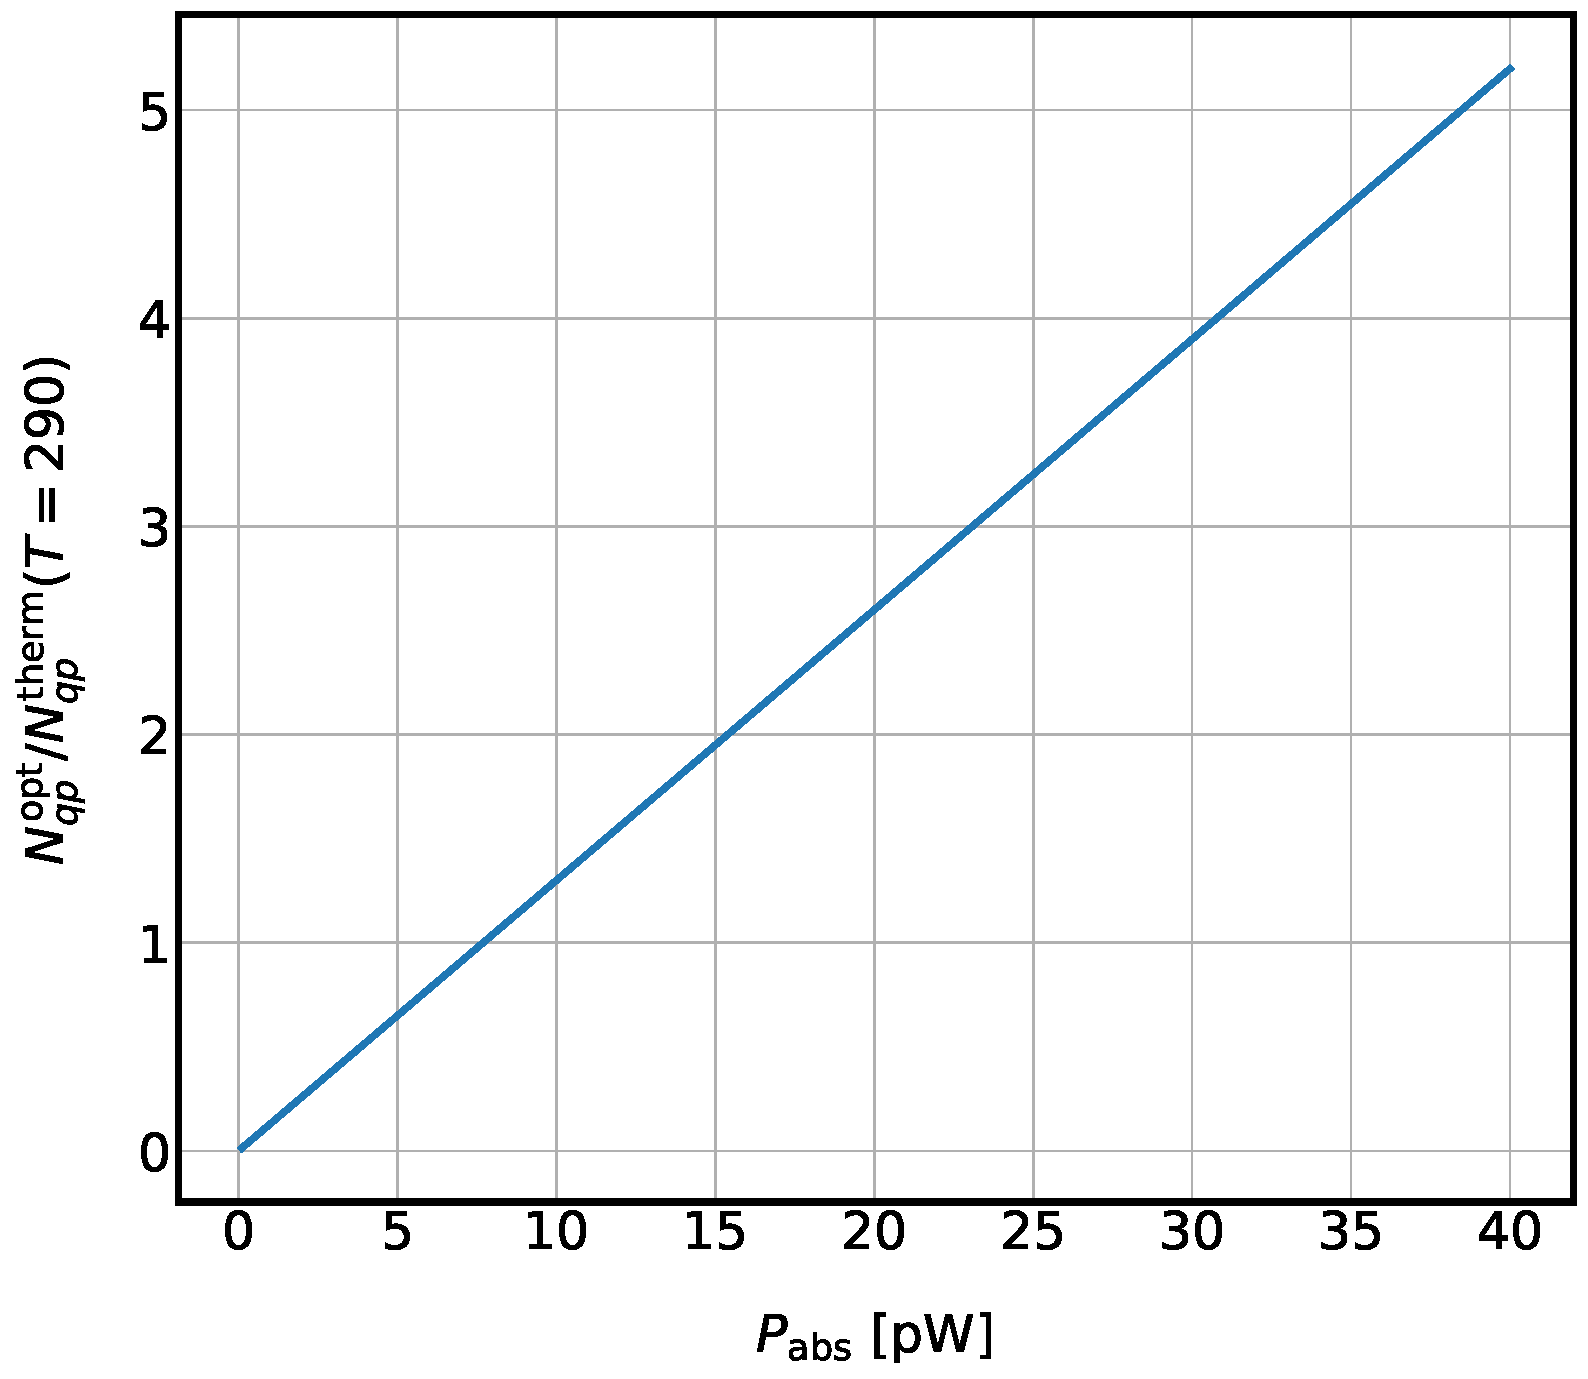
\includegraphics[width=0.8\textwidth]{figures/kid_model/Nqp_ratio}
\caption[~The ratio of the number of optically generated to thermally generated QP as a function of absorbed optical power.]{The ratio of the number of optically generated QP to thermally generated QP, $N_{qp,\mathrm{opt}}/N_{qp,\mathrm{therm}}$, as a function of \gls{Pabs}. \gls{Tbase} is fixed at 290~mK.}
\label{fig:Nrat}
\end{figure}

The ratio $\gls{Nqp}(P)/\gls{Nqp}(T = 290)$ is shown in Figure~\ref{fig:Nrat} for a range of \gls{Pabs}, with $\gls{Tbase} = 290$~mK. Using Equations~\ref{eq:Nqp_T} and~\ref{eq:Nqp_P} to express the total number of QP $N_{qp,\mathrm{,tot}}$, the band gap energy can now be expressed as a function of both \gls{Tc} and \gls{Pabs}:

% Delta as function of Nqp_tot
\begin{equation}
 \Delta(T,P) = \frac{\gls{Delta}}{2}\left( 1 + \sqrt{1 - \frac{2\gls{Nqp}_{\mathrm{,tot}}} {\Sigma\gls{N0}\gls{Delta}}} \right)
\end{equation}

\subsection{The Two-Fluid Model}\label{two_fluid_model}

Several of the KID parameters discussed in the following sections depend on the conductivity $\sigma$ of the superconductor. Here we describe the two-fluid model of conductivity (\citet{glover1957conductivity,mattis1958theory}), which relates the Drude conductivity \gls{sig_d} in a normal conductor to the CPs and QP of a superconductor.

In a conductor, the equation of motion for a charge carrier is:

\begin{equation}
  \gls{mstar}\dot{v} = -eE - \frac{\gls{mstar}v}{\gls{tau_s}}
\end{equation}

where $\omega$ is the frequency of a time-varying electromotive force (EMF) being applied to the circuit, \gls{mstar} is the effective mass of the charge carrier, and $\boldsymbol{v}$ is their drift velocity ($\propto e^{j\omega\gls{tau_s}}$). The second term on the right-hand side of the equation is a damping term which accounts for charges scattering off of the lattice, with \gls{tau_s} being the characteristic time between collisions. Ohm's Law provides the relation between conductivity and current density: $J = \gls{sig_d} E$, with $J = n_{e}ev$.

Inserting these relations into the equation of motion, and solving for \gls{sig_d} yields the Drude conductivity:

\begin{equation}\label{eq:drude}
  \begin{aligned}
  \gls{sig_d}(\omega) &= \frac{n_{e}e^{2}\gls{tau_s}}{m_{e}}\frac{1}{1 + j\omega\tau} \\
                 &= \frac{\sigma_{n}}{1 + j\omega\gls{tau_s}} \\
                 &= \frac{\gls{sig_n}}{1 + \omega^{2}\gls{tau_s}^{2}} - j\frac{\gls{sig_n}\gls{tau_s}}{1 + \omega^{2}\gls{tau_s}^{2}} \\
                 &= \gls{sig1} - j\gls{sig2}
  \end{aligned}
\end{equation}

where \gls{sig_n} is the normal conductivity, $\gls{sig_n} = n_{e}e^{2}\gls{tau_s}/\gls{mstar}$. In a normal metal, \gls{tau_s} is small enough so that $\gls{sig_d} \approx \gls{sig_n}$ is negligible at frequencies $\omega$ below the optical range. For $kT \ll \gls{Delta}$ and $\hbar \omega \ll \gls{Delta}$, the real and imaginary conductivities can be written as \citep{gao2008physics}:

% sig1 thermal
\begin{equation}
  \gls{sig1}(\gls{nqp}, T)_{\mathrm{therm}} = \frac{4\gls{sig_n}\gls{Delta}}{\hbar \omega}e^{-\frac{\gls{Delta} - \upmu^{*}}{kT}}\sinh(\xi)\gls{K0}(\xi)
\end{equation}

% sig2 thermal
\begin{equation}
  \gls{sig2}(\gls{nqp}, T)_{\mathrm{therm}} = \frac{\gls{sig_n}\gls{Delta}}{\hbar \omega}\Bigg[ 1 - \sqrt{ \frac{ 2\pi kT }{ \gls{Delta} } } e^{-\frac{\gls{Delta}}{kT}}
   - 2e^{ \frac{\gls{Delta}}{kT}} e^{-\xi} \gls{I0} \Bigg]
\end{equation}

% sig 1 optical
\begin{equation}
  \gls{sig1}(\gls{nqp}, T)_{\mathrm{opt}} = \frac{2\gls{Delta}}{\hbar \omega} \frac{ \gls{nqp}} { 2\gls{N0}\sqrt{\pi kT\gls{Delta}}}\sinh(\xi)\gls{K0}(\xi)
\end{equation}

% sig2 optical
\begin{equation}
  \gls{sig2}(\gls{nqp}, T)_{\mathrm{opt}} = \frac{ \pi\gls{Delta} }{ \hbar\omega } \Bigg[ 1 - \frac{ \gls{nqp} }{ 2\gls{N0}\gls{Delta} } \left( 1 +
  \sqrt{ \frac{ 2 \gls{Delta} }{ \pi kT } } e^{-\xi} \gls{I0} \right) \Bigg]
\end{equation}

Figure~\ref{fig:sig_ratio_T} shows the ratio of \gls{sig1} to \gls{sig2} as a function of \gls{Tbase} ($\gls{Pabs} = 0$). The ratio asymptotically decays to zero for $T \gtrsim 250$~mK. The ratio of \gls{sig1} to \gls{sig2} as a function of \gls{Pabs} ($\gls{Tbase} = 290$~mK) is shown in Figure~\ref{fig:sig_ratio_P}. The ratio falls below one for $\gls{Pabs} \gtrsim 12$~pW.

\begin{figure}[!htbp]
\centering
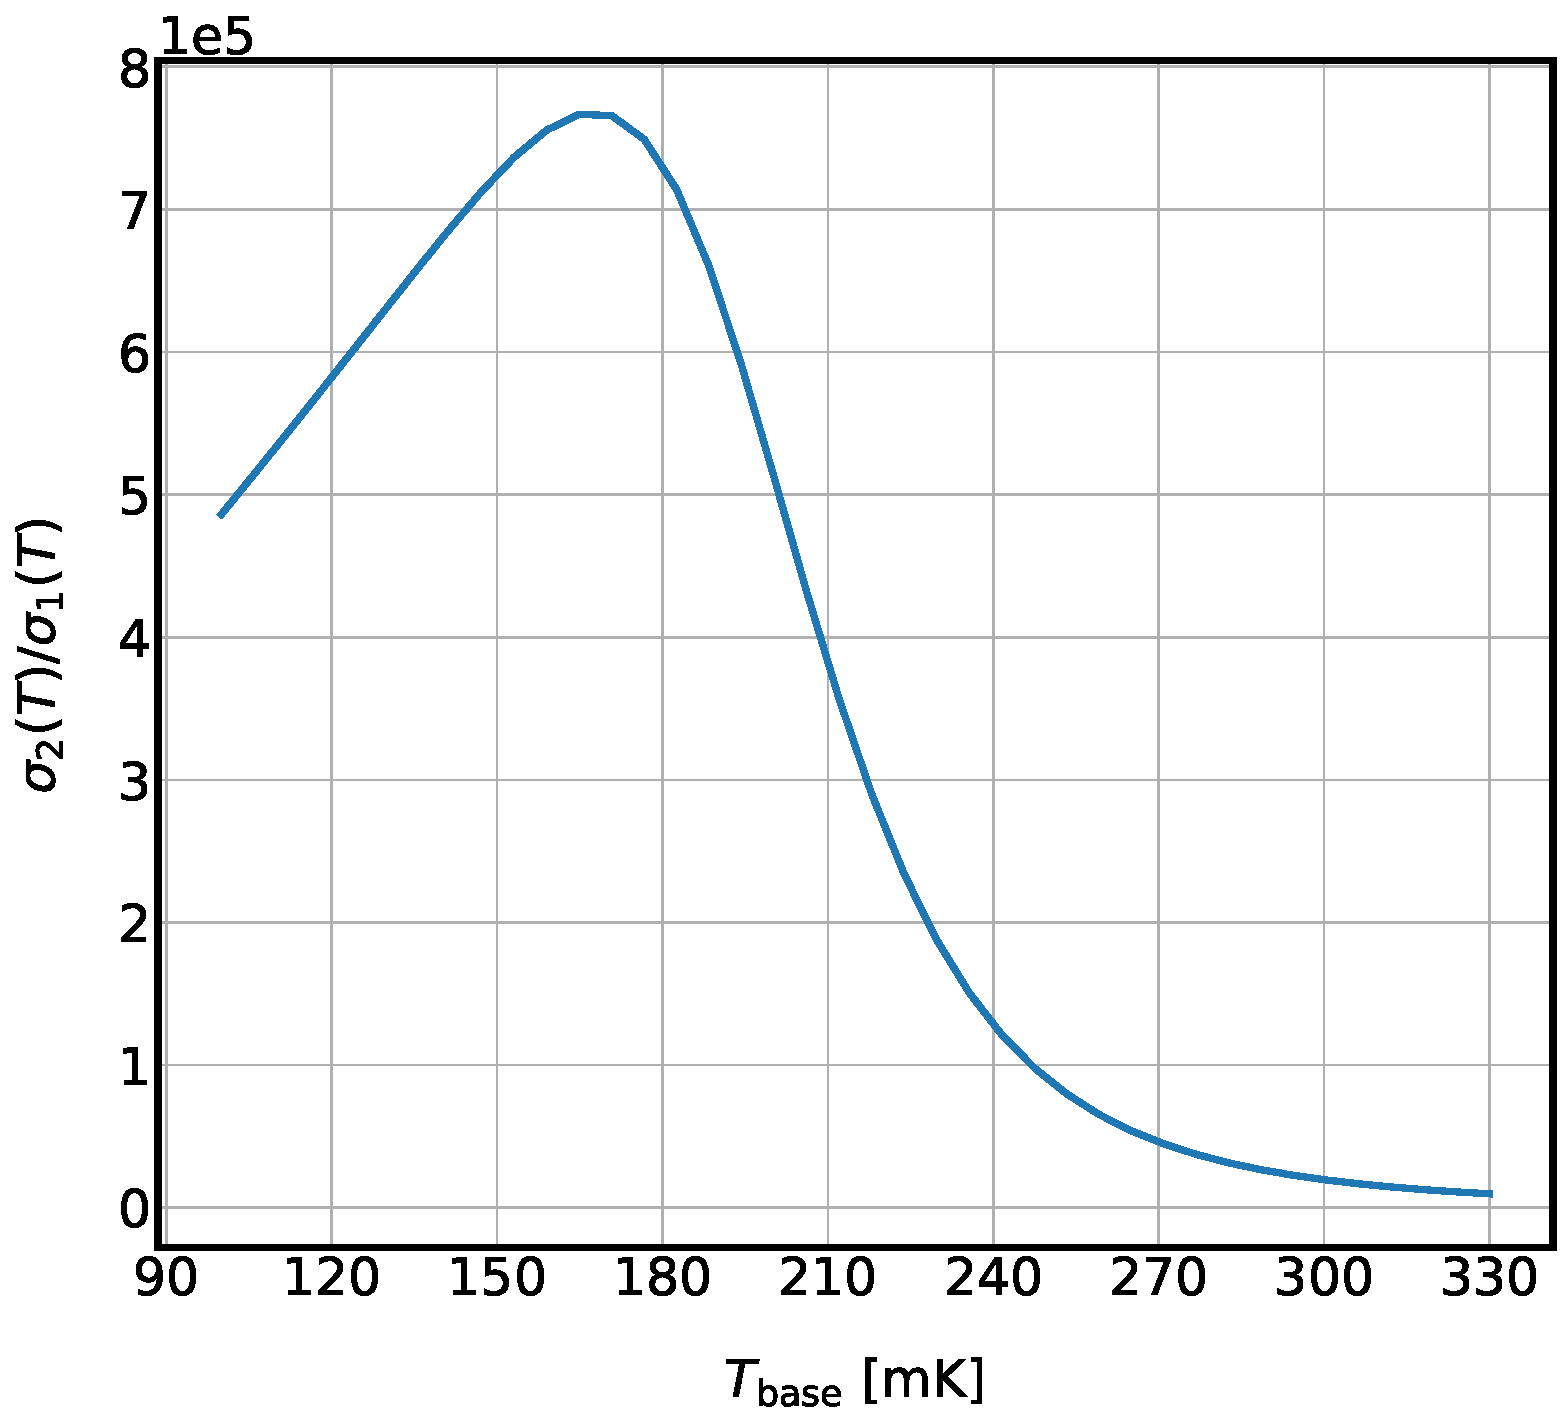
\includegraphics[width=0.8\textwidth]{figures/kid_model/sig_ratio_T}
\caption[~The ratio of \macrocapwrap{\gls{sig1}} to \macrocapwrap{\gls{sig2}} as a function of base temperature.]{The ratio of \gls{sig1} to \gls{sig2} as a function of base temperature.}
\label{fig:sig_ratio_T}
\end{figure}

\begin{figure}[!htbp]
\centering
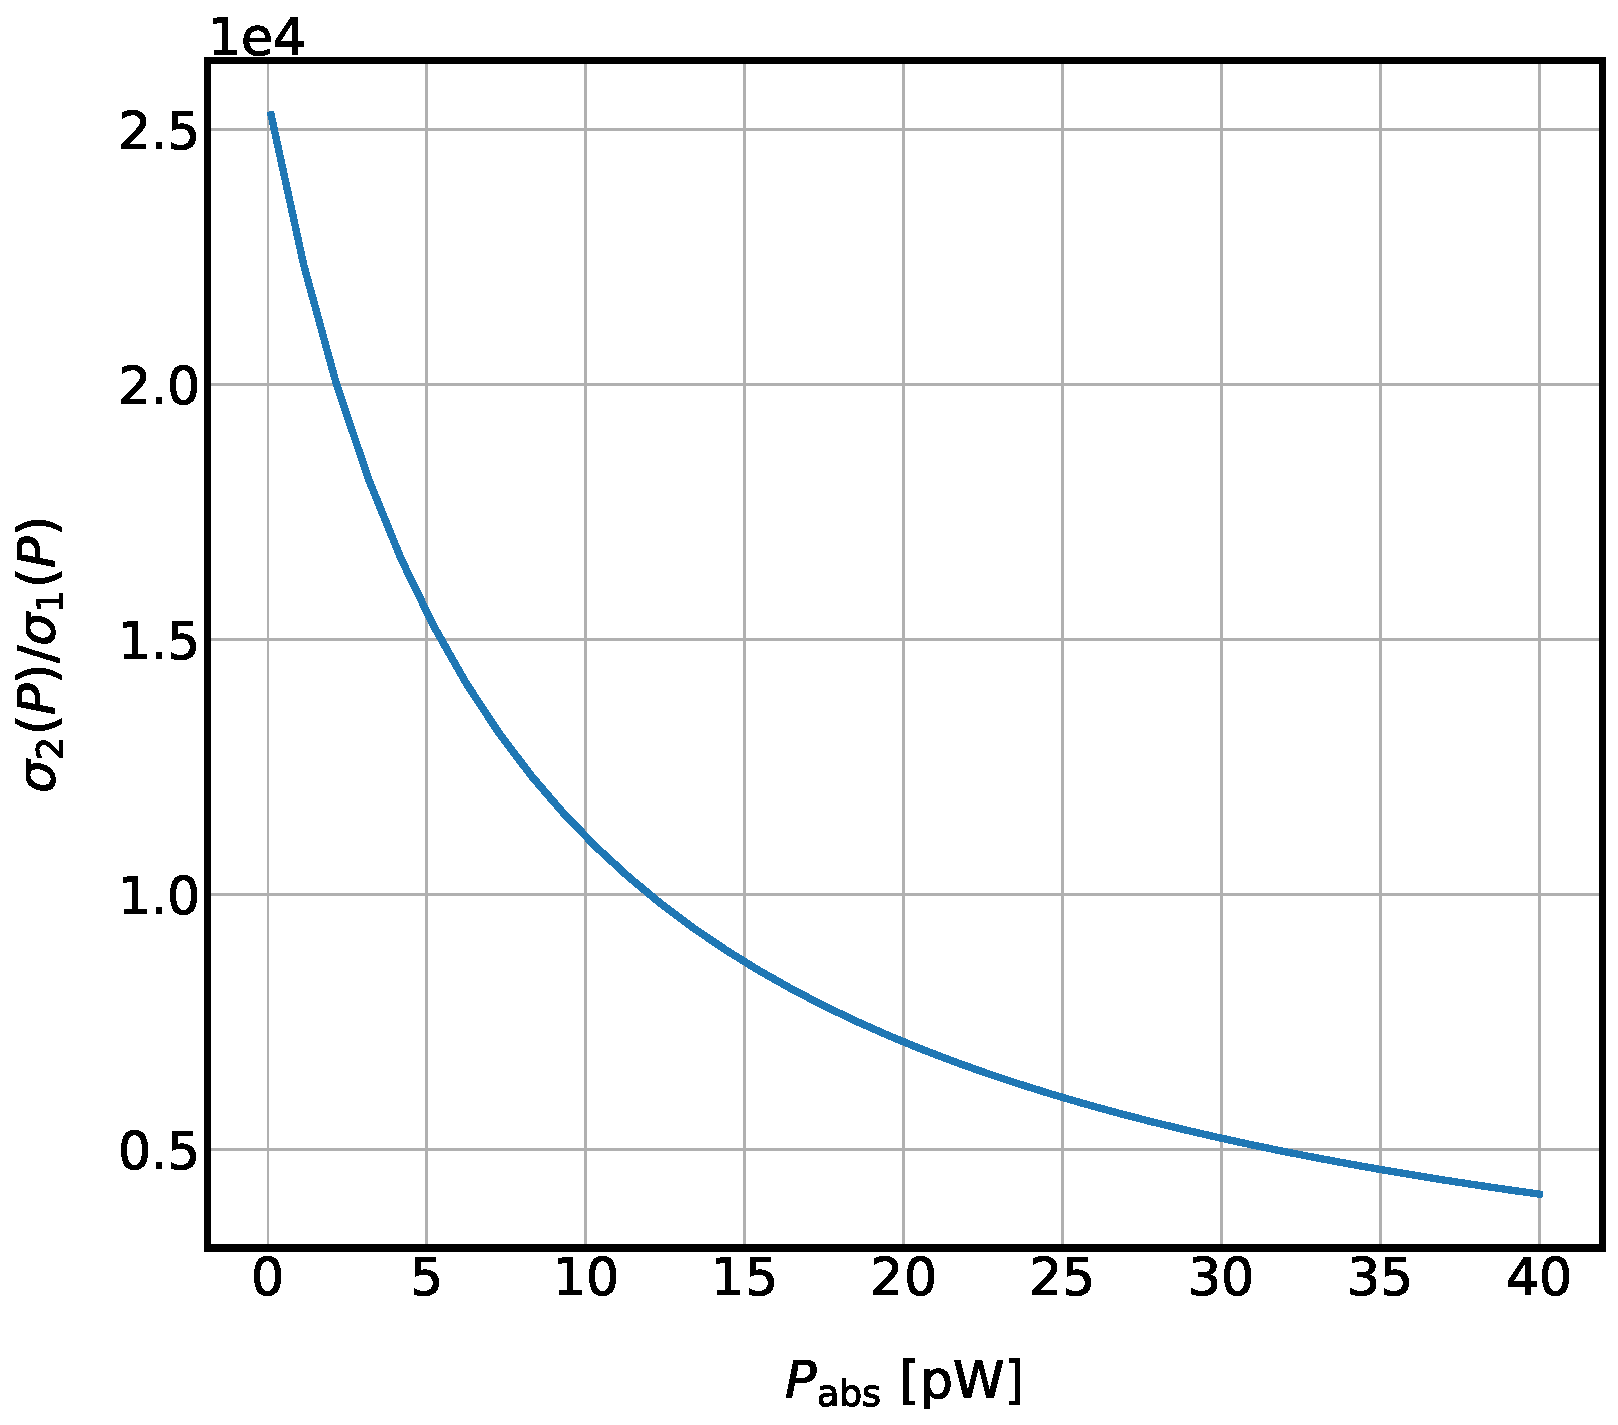
\includegraphics[width=0.8\textwidth]{figures/kid_model/sig_ratio_P}
\caption[~The ratio of \macrocapwrap{\gls{sig1}} to \macrocapwrap{\gls{sig2}} as a function of absorbed optical power at a base temperature of 290~mK.]{The ratio of \macrocapwrap{\gls{sig1}} to \macrocapwrap{\gls{sig2}} as a function of absorbed optical power, at a base temperature of 290~mK.}
\label{fig:sig_ratio_P}
\end{figure}

where $\upmu^{*}$ is an effective chemical potential which is added to the Fermi distribution function to account for QP generation due to pair breaking (for a derivation, see \citet{PhysRevLett.28.1559,gao2008physics}).

% mu thermal
\begin{equation}
  \upmu^{*}_{\mathrm{therm}} = kT\ln\left( \frac{\gls{nqp}}{2\gls{N0}\sqrt 2\pi kT\gls{Delta}} \right) + \gls{Delta}
\end{equation}

% mu optical
\begin{equation}
  \upmu^{*}_{opt} = kT\ln \left( \frac{\gls{Nqp}^{tot}}{2V\gls{N0}\sqrt{2\pi kT\Delta}} \right) + \Delta
\end{equation}

where $\omega$ is the KID resonant frequency, $\gls{sig_n}$ is the normal conductivity of the material, $\xi = \hbar \omega/2kT$, \gls{K0} is the Modified Bessel function of the second kind of order zero, and \gls{I0} is the Modified Bessel function of order zero.

\section{Kinetic Inductance} \label{sec:kinetic_inductance}

When a voltage is applied to a closed circuit, current does not start to flow instantaneously. The reason for this is that some energy from the applied voltage must first be stored in (or extracted from, if the sign of the voltage is reversed) a B-field, via the inductance $L$. Inductance is defined as the ratio of the rate of change of current, to the applied voltage: $L = \frac{V}{dI/dt}$ [$\Omega$/Hz]. The energy stored in the inductance is $E_{L} = \frac{1}{2}LI^{2}$. The magnetic inductance \gls{Lm} of a superconducting film depends solely on its geometric parameters: Length $l$, width $w$, thickness $t$.

In all conductors there is an additional form of inductance, known as the KI (KI) $L_{k}$. The total inductance is the sum of the magnetic (or geometric) and kinetic inductances:

% total inductance
\begin{equation}
  L_{\mathrm{tot}} = \gls{Lm} + L_{k}
\end{equation}

It's useful to define a KI fraction, as:

\begin{equation}
  \gls{alphaKI} = \frac{L_{k}}{L_{\mathrm{tot}}}
\end{equation}

The KI arises from the inertia of the CPs. As charge carriers scatter (or break apart, in the case of CPs), the kinetic energy (velocity) of the remaining charge carriers must increase in order to keep the current constant. This increase in velocity cannot happen instantly. Therefore, if an AC current is circulated through a superconducting circuit, and the KI is increased, the the current undergoes a phase shift. There is a also a maximum velocity imposed upon the charge carriers, corresponding to the critical, or pair-breaking current of the material, which is described in the Ginzberg-Landau theory (GL) of superconductivity (see Section~\ref{nonlinearKI}) \citep{tinkham2004introduction}.

From an energy standpoint, an expression for the KI can be derived by equating the energy in the KI to the kinetic energy of a CP:

\begin{equation}
  \begin{aligned}
  \frac{1}{2}L_{k}I^{2} &= \frac{1}{2}(2m_{e})v_{cp}^{2}N_{cp}\\
                        &= m_{e}^{2}v_{cp}^{2}n_{cp}lA
  \end{aligned}
\end{equation}

where $A = wlt$ is the cross-sectional area of the transmission line (TL), $I_{s}$ is the supercurrent, $v_{cp}$ is the CP velocity and $N_{cp}$ is the total number of CPs. Defining the supercurrent as

\begin{equation}
  \begin{aligned}
  I_{s} = \frac{1}{2}n_{cp}(2e)v_{cp}A
  \end{aligned}
\end{equation}

, the KI per unit length is

\begin{equation} \label{eq:KI_per_length}
  \gls{Lk_per_l} = \frac{m_{e}}{n_{cp}e^{2}A}
\end{equation}

The KI can also be understood by considering the impedance. Because CPs are collisionless, their scattering time \gls{tau_s} is infinite. Taking the limit of Equation~\ref{eq:drude} as \gls{tau_s} goes to infinity:

\begin{equation}
    \begin{aligned}
    \lim_{\gls{tau_s} \to \infty} \gls{sig_d}(\omega) &= -j\frac{n_{e}e^{2}}{m_{e}\omega}\\
    &= \gls{sig2}
    \end{aligned}
\end{equation}

Therefore, the KI per unit length is

\begin{equation}
  \gls{Lk_per_l}(\omega) = \frac{1}{\gls{sig2}\omega t}
\end{equation}

and the KI per square is

\begin{equation}
  \gls{Lk_per_sq}(\omega) = \frac{1}{\gls{sig2}\omega t}
\end{equation}

The impedance of the superconducting film can be written as a function of the conductivity:

\begin{equation}\label{eq:Z}
  \begin{aligned}
  Z(\omega) &= \frac{1}{t\sigma(\omega)}\\
            &= \frac{1}{t}\left( \frac{\gls{sig1}}{\gls{sig2}^{2}} - j\gls{sig2}^{-1}\right)\\
            &= \mathcal{R} + j\omega\gls{Lk_per_sq}
  \end{aligned}
\end{equation}

where $\mathcal{R}$ is the resistance per square.

Then,

\begin{equation}
  \gls{Lk_per_sq}(\omega) = \frac{1}{\gls{sig2}\omega t}
\end{equation}

Using the fact that in the low-frequency limit ($\hbar\omega \ll kT$), Mattis-Bardeen (MB) theory allows the complex conductivity to be expressed as (\citet{mauskopf2018transition,annunziata2010tunable}):

\begin{equation}
  \gls{sig2} = \frac{\gls{sig_n}\pi\Delta}{\hbar\omega}\tanh \left(\frac{\gls{Delta}}{2kT}\right)
\end{equation}

and the sheet resistance of the film in the normal state is \gls{Rsq} = 1/\gls{sig_n}t, the KI per square becomes:

\begin{equation} \label{eq:Lk_Rsq}
  \gls{Lk_per_sq}(T,P) = \frac{\hbar\gls{Rsq}}{\pi\Delta(T,P)}
\end{equation}

Equation~\ref{eq:Lk_Rsq} illustrates the fact that materials with higher normal state sheet resistivity, and/or smaller band gaps, have higher intrinsic KI fractions \gls{alphaKI}. Figures~\ref{fig:alpha_T} and~\ref{fig:alpha_P} show \gls{alphaKI} as a function of \gls{Tbase} and \gls{Pabs}. The KI fraction is expontial in \gls{Tbase}, but linear in \gls{Pabs}.

\begin{figure}[!htbp]
\centering
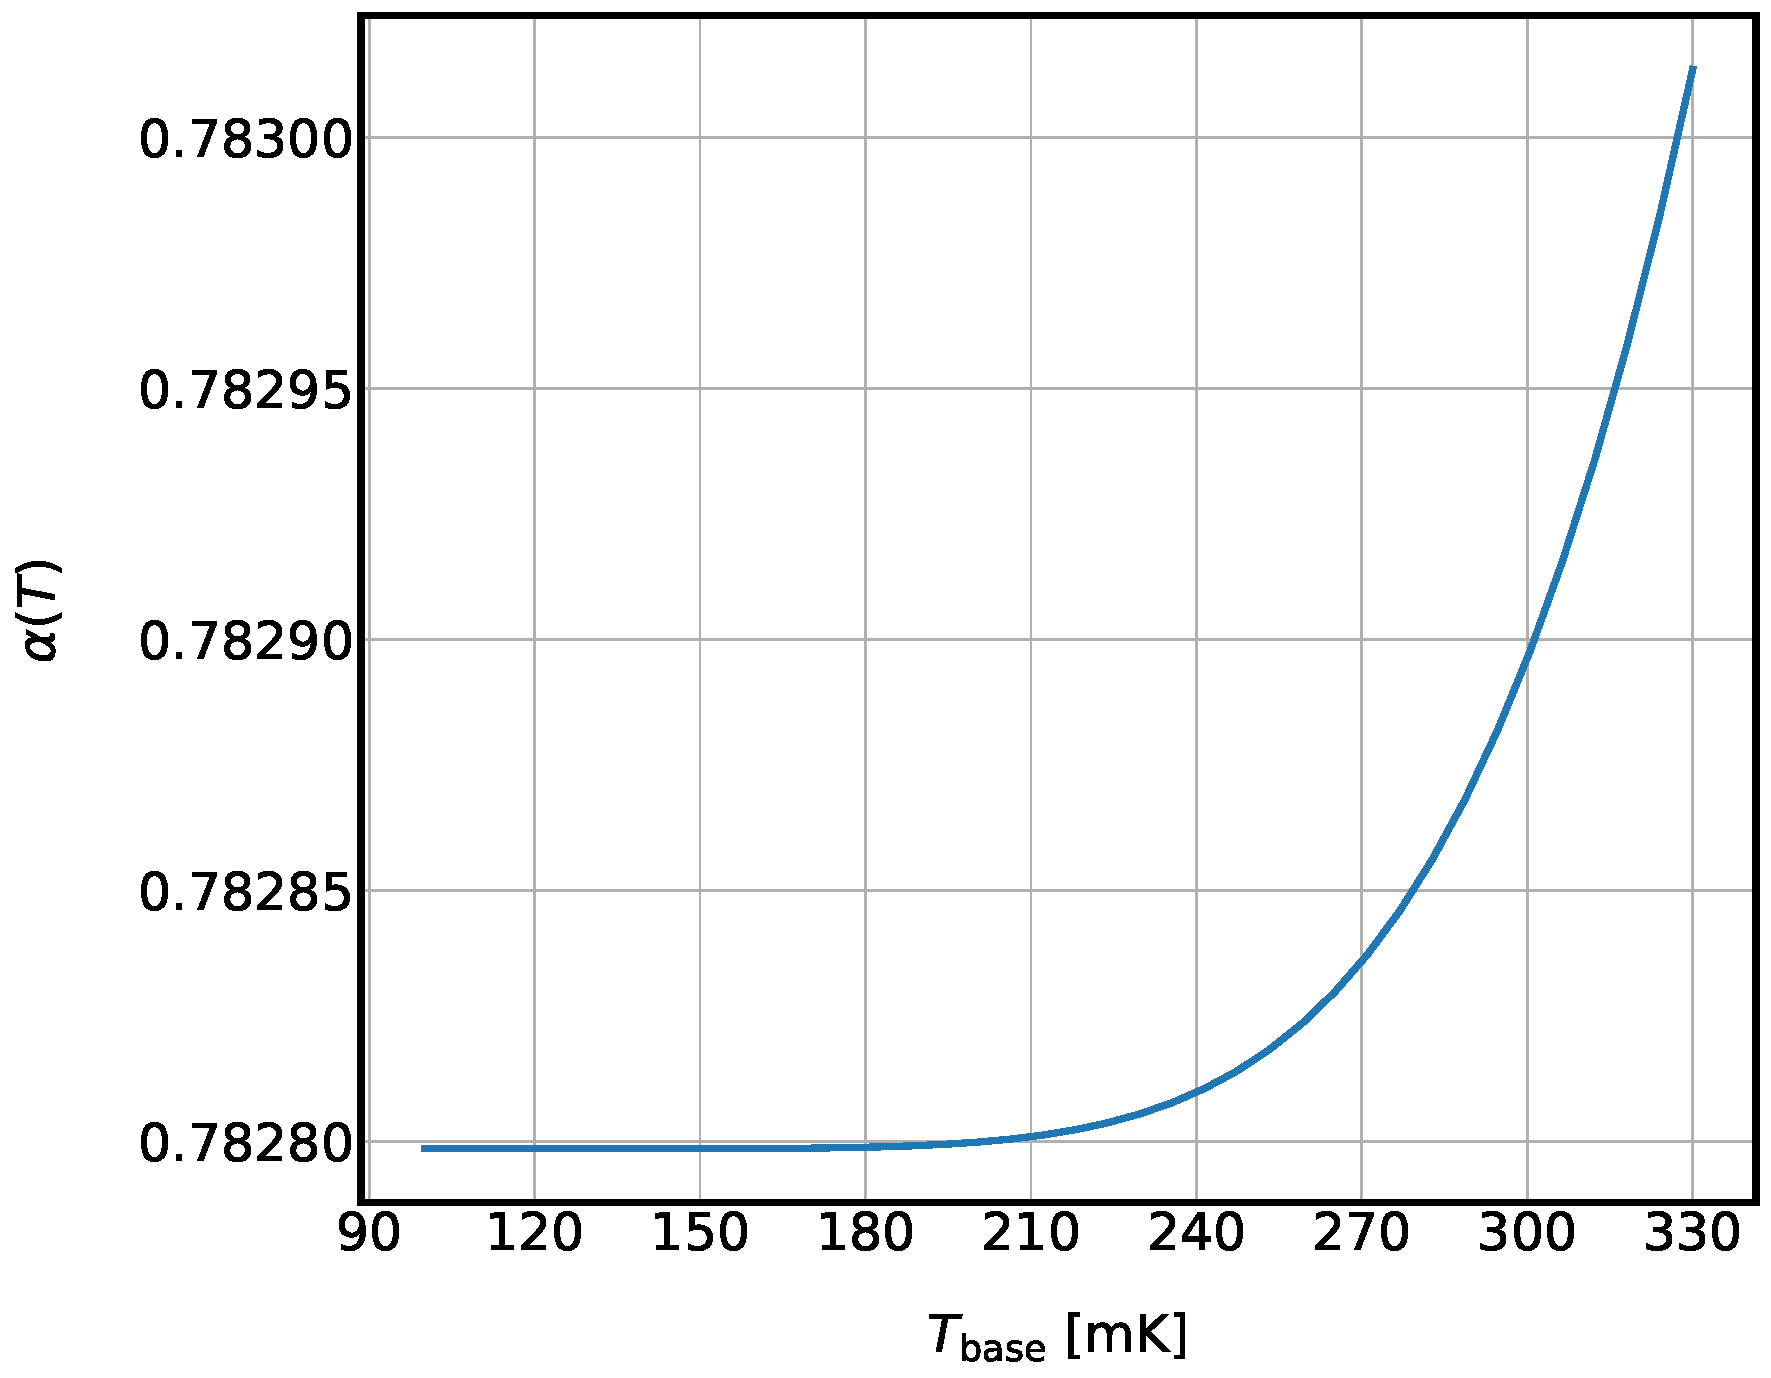
\includegraphics[width=0.8\textwidth]{figures/kid_model/alpha_T}
\caption[~\macrocapwrap{\gls{alphaKI}} as a function of base temperature.]{The kinetic inductance ratio \gls{alphaKI} as a function of base temperature.}
\label{fig:alpha_T}
\end{figure}

\begin{figure}[!htbp]
\centering
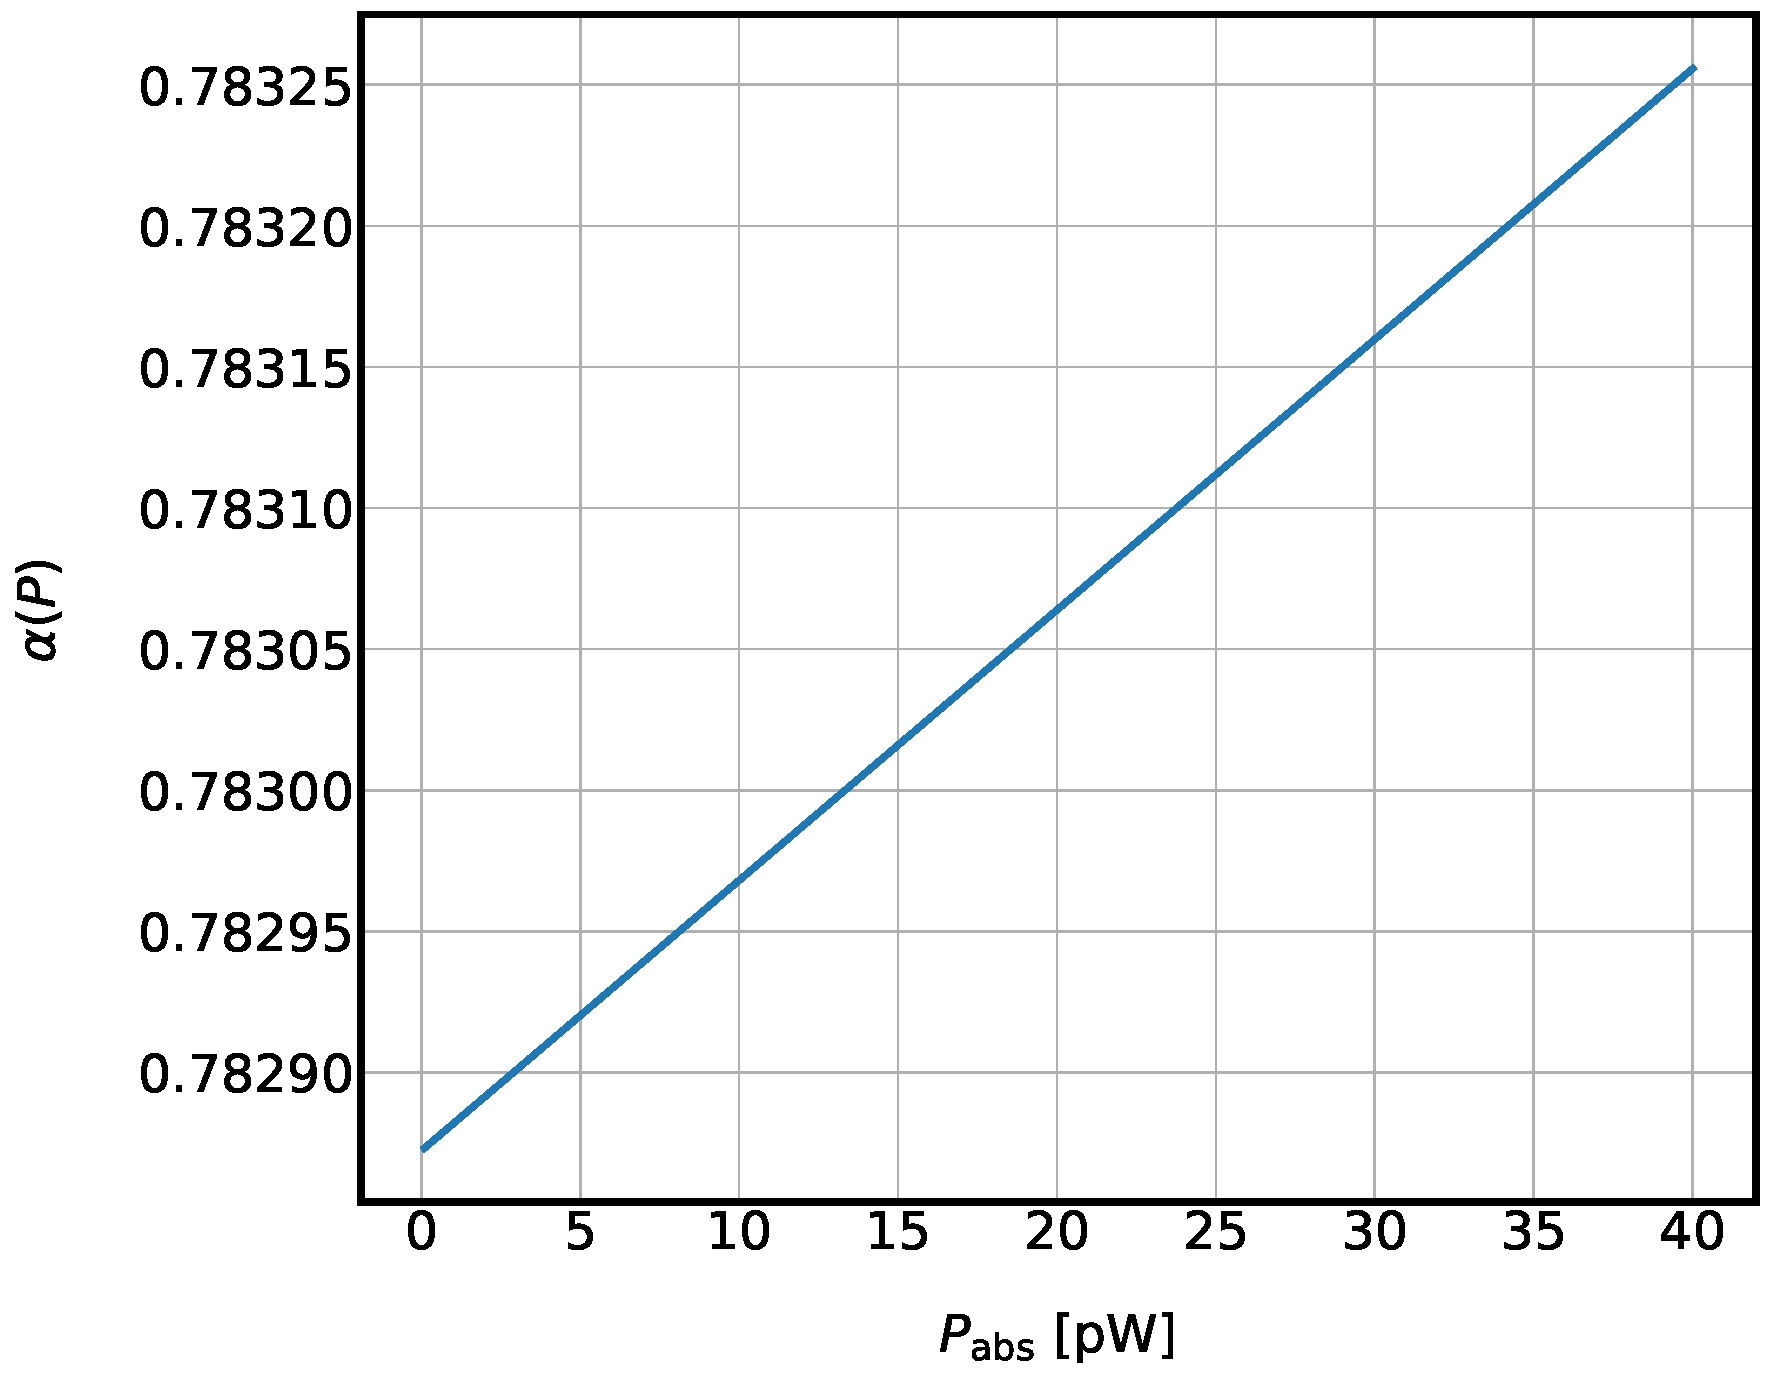
\includegraphics[width=0.8\textwidth]{figures/kid_model/alpha_P}
\caption[~\macrocapwrap{\gls{alphaKI}} as a function of absorbed power.]{The kinetic inductance fraction \gls{alphaKI} as a function of optical power.}
\label{fig:alpha_P}
\end{figure}

\section{Principle LEKID Parameters}\label{sec:kid_params}

In the previous sections, several superconducting device properties were derived as functions of base temperature \gls{Tbase} and absorbed optical power \gls{Pabs}. Now, we introduce a circuit model for a lumped-element KID (LEKID), and derive the temperature and power dependence of several instrinsic and empirical (determined from measurements) parameters.

\subsection{Intrinsic and Empirical Parameters}

A LEKID is a capacitively-coupled lumped-element resonant circuit (tank circuit). It has five intrinsic circuit parameters. These are:

\begin{itemize}[label={},nosep]
  \item $L_{\mathrm{tot}}$ \quad The total resonator inductance
  \item $C_{r}$ \quad The resonator capacitance
  \item $C_{c}$ \quad The coupling capacitance
  \item $R_{\mathrm{eff}}$ \quad An effective resistance, in series with $L_{\mathrm{tot}}$, which accounts for the real part of the resonator impedance
  \item $Z_{0}$ \quad The feedline impedance
\end{itemize}

\begin{figure}[!htbp]
\centering
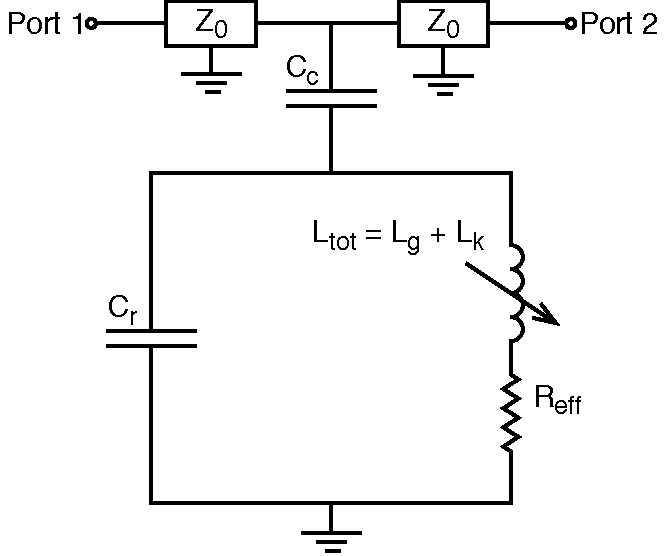
\includegraphics[width=0.5\textwidth]{figures/kid_model/mkid_schematic}
\caption{~A schematic of a single LEKID.}
\label{fig:lekid_schematic}
\end{figure}

Figure~\ref{fig:lekid_schematic} shows a schematic which illustrates how a LEKID is constructed from the basic elements listed above.

There are four principle empirical parameters:

\begin{itemize}[label={},nosep]
  \item \gls{Qr} \quad The resonator quality factor
  \item \gls{Qc} \quad The coupling quality factor
  \item $\omega_{0}$ \quad The resonant frequency
  \item \gls{asym} \quad A parameter which accounts for a frequency dependent asymmetry in resonator impedance
\end{itemize}

The resonant frequency is set by the total inductance and resonator capacitance:

\begin{equation}\label{eq:f0}
  \omega_{0} = \frac{1}{\sqrt{\mathcal{L}_{\mathrm{tot}}\mathcal{C}_{r}}}
\end{equation}

From the perspective of a microwave carrier tone which is input to the feedline at frequency $\omega_{c} = 2\pi f_{c}$, the LEKID acts as a frequency dependent shunt impedance to ground. The resonant frequency of the LEKID is changed by modulating the KI, with a combination of changes in absorbed optical power, base temperature, and microwave probe tone power. Taking the derivative of Equation~\ref{eq:f0} with respect to \gls{Lk_per_l}, and defining the resonator capacitance as $C_{r} = \frac{1}{L_{\mathrm{tot}}\omega_{0}^{2}}$,

\begin{equation}
 \frac{df_{0}}{d\gls{Lk_per_l}} = \frac{-\alpha f_{0}}{2\gls{Lk_per_l}}
\end{equation}

The asymmetry parameter is defined as $\gls{asym} = \frac{C_{r}}{C_{c}\gls{Qi}}$
where \gls{Qi} is the internal quality factor \citep{mauskopf2018transition}. The internal quality factor is itself defined as:

% Qi
\begin{equation}\label{eq:Qi}
  \gls{Qi} = \frac{\Im(Z_{r})}{\Re(Z_{r})} = \frac{\omega_{c}L_{\mathrm{tot}}}{R_{\mathrm{eff}}} = \frac{\omega_{c} E_{r}}{P_{\mathrm{diss}}}
\end{equation}

where $E_{r}$ is the stored (internal) energy of the resonator, and $P_{\mathrm{diss}}$ is the dissipated power, or energy dissipated per cycle of the carrier tone at frequency $\omega_{c}$. The couping quality factor is (see \citet{barry2014development}):

\begin{equation} \label{eq:Qc}
  \gls{Qc} = \frac{2(C_{r} + C_{c})}{\omega_{0}C_{c}^{2}Z_{0}}
\end{equation}

The measured resonator quality factor, $Q_{r}$, is related to the internal and coupling quality factors as:
% Qr, measured resonator quality factor
\begin{equation}
  \frac{1}{\gls{Qr}} = \frac{1}{\gls{Qi}} + \frac{1}{\gls{Qc}} + \frac{1}{Q_{\mathrm{loss}}}
\end{equation}

where $Q_{\mathrm{loss}}$ is an external loss factor, typically of $\mathcal{O}(10^{6})$, which accounts for parasitic loss, including parasitic capacitance and inductance.

Figures~\ref{fig:Qr_T} and \ref{fig:Qr_P} show \gls{Qr} as a function of \gls{Tbase} and \gls{Pabs}. While $\gls{Qr}(P)$ decreases monotonically with increasing absorbed optical power, $\gls{Qr}(T)$ does not. Starting at $\gls{Tbase} = 90$~mK, $\gls{Qr}(T)$ first increases with base temperature, reaching a maximum at $\gls{Tbase} \sim 180$~mK, before decreasing almost linearly.

\begin{figure}[!htbp]
\centering
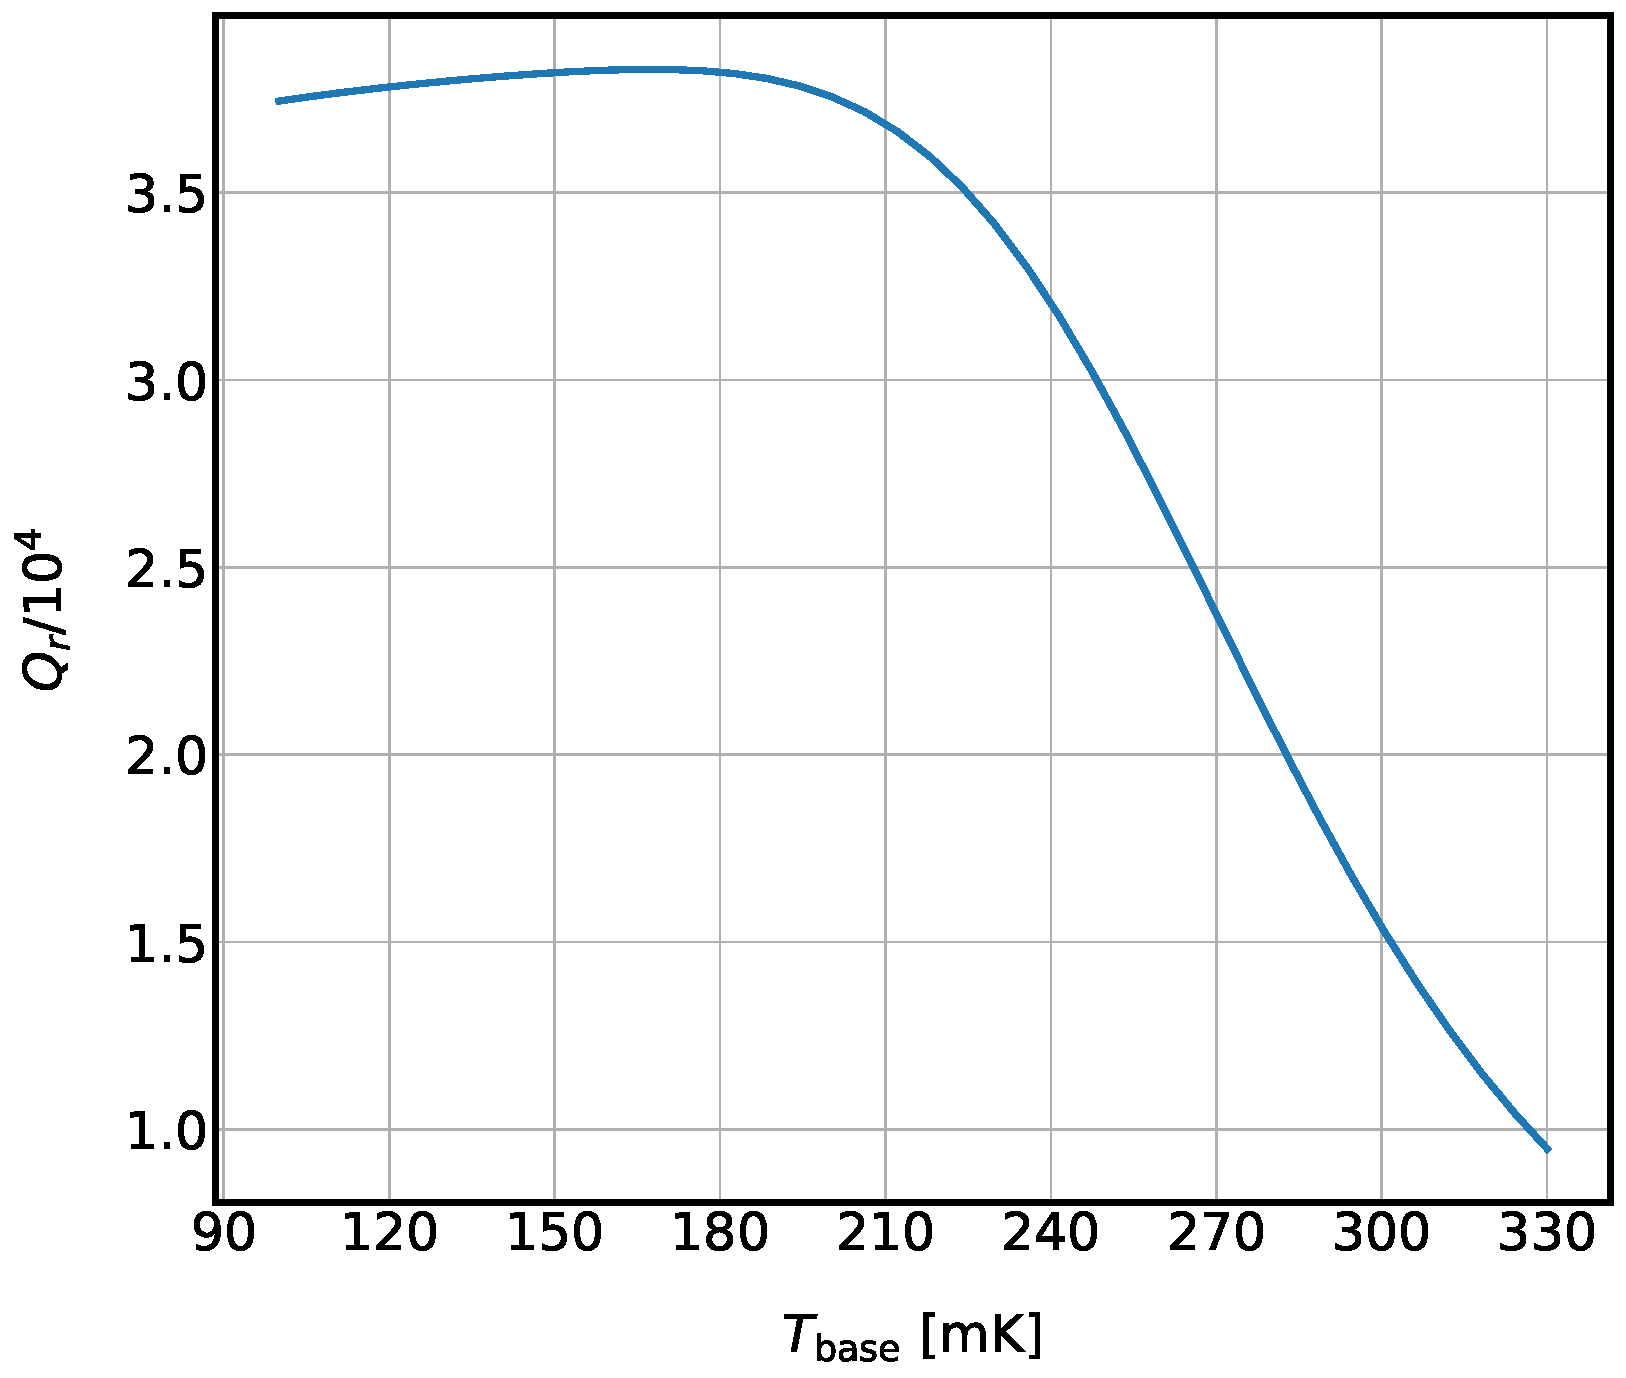
\includegraphics[width=0.8\textwidth]{figures/kid_model/Qr_v_T}
\caption[~Simulated \macrocapwrap{$Q_{r}$} as a function of base temperature.]{Simulated $Q_{r}$ as a function of base temperature.}
\label{fig:Qr_T}
\end{figure}

\begin{figure}[!htbp]
\centering
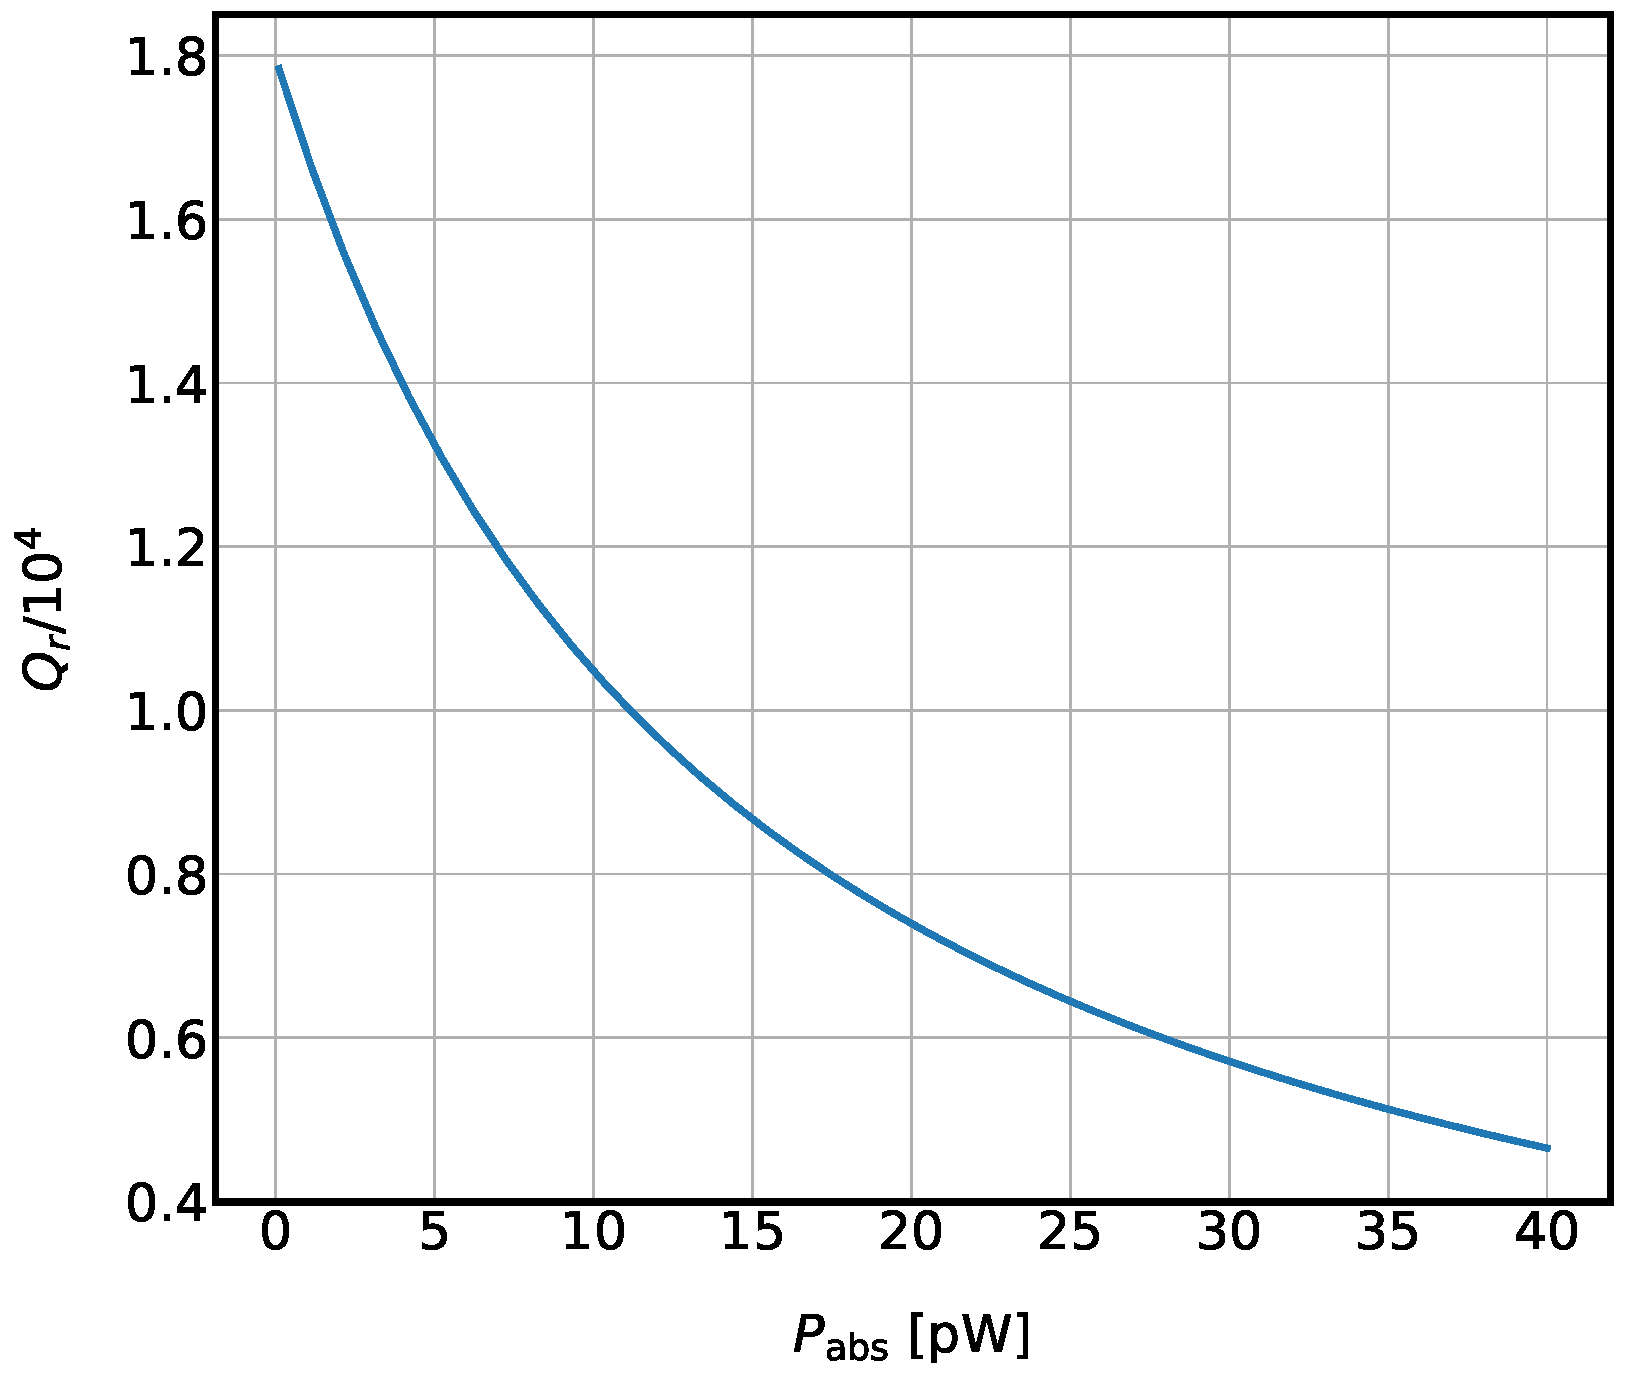
\includegraphics[width=0.8\textwidth]{figures/kid_model/Qr_v_P}
\caption[~Simulated \macrocapwrap{$Q_{r}$} as a function of optical power.]{Simulated $Q_{r}$ as a function of optical power.}
\label{fig:Qr_P}
\end{figure}

\begin{comment}
\begin{figure}[!htbp]
\centering
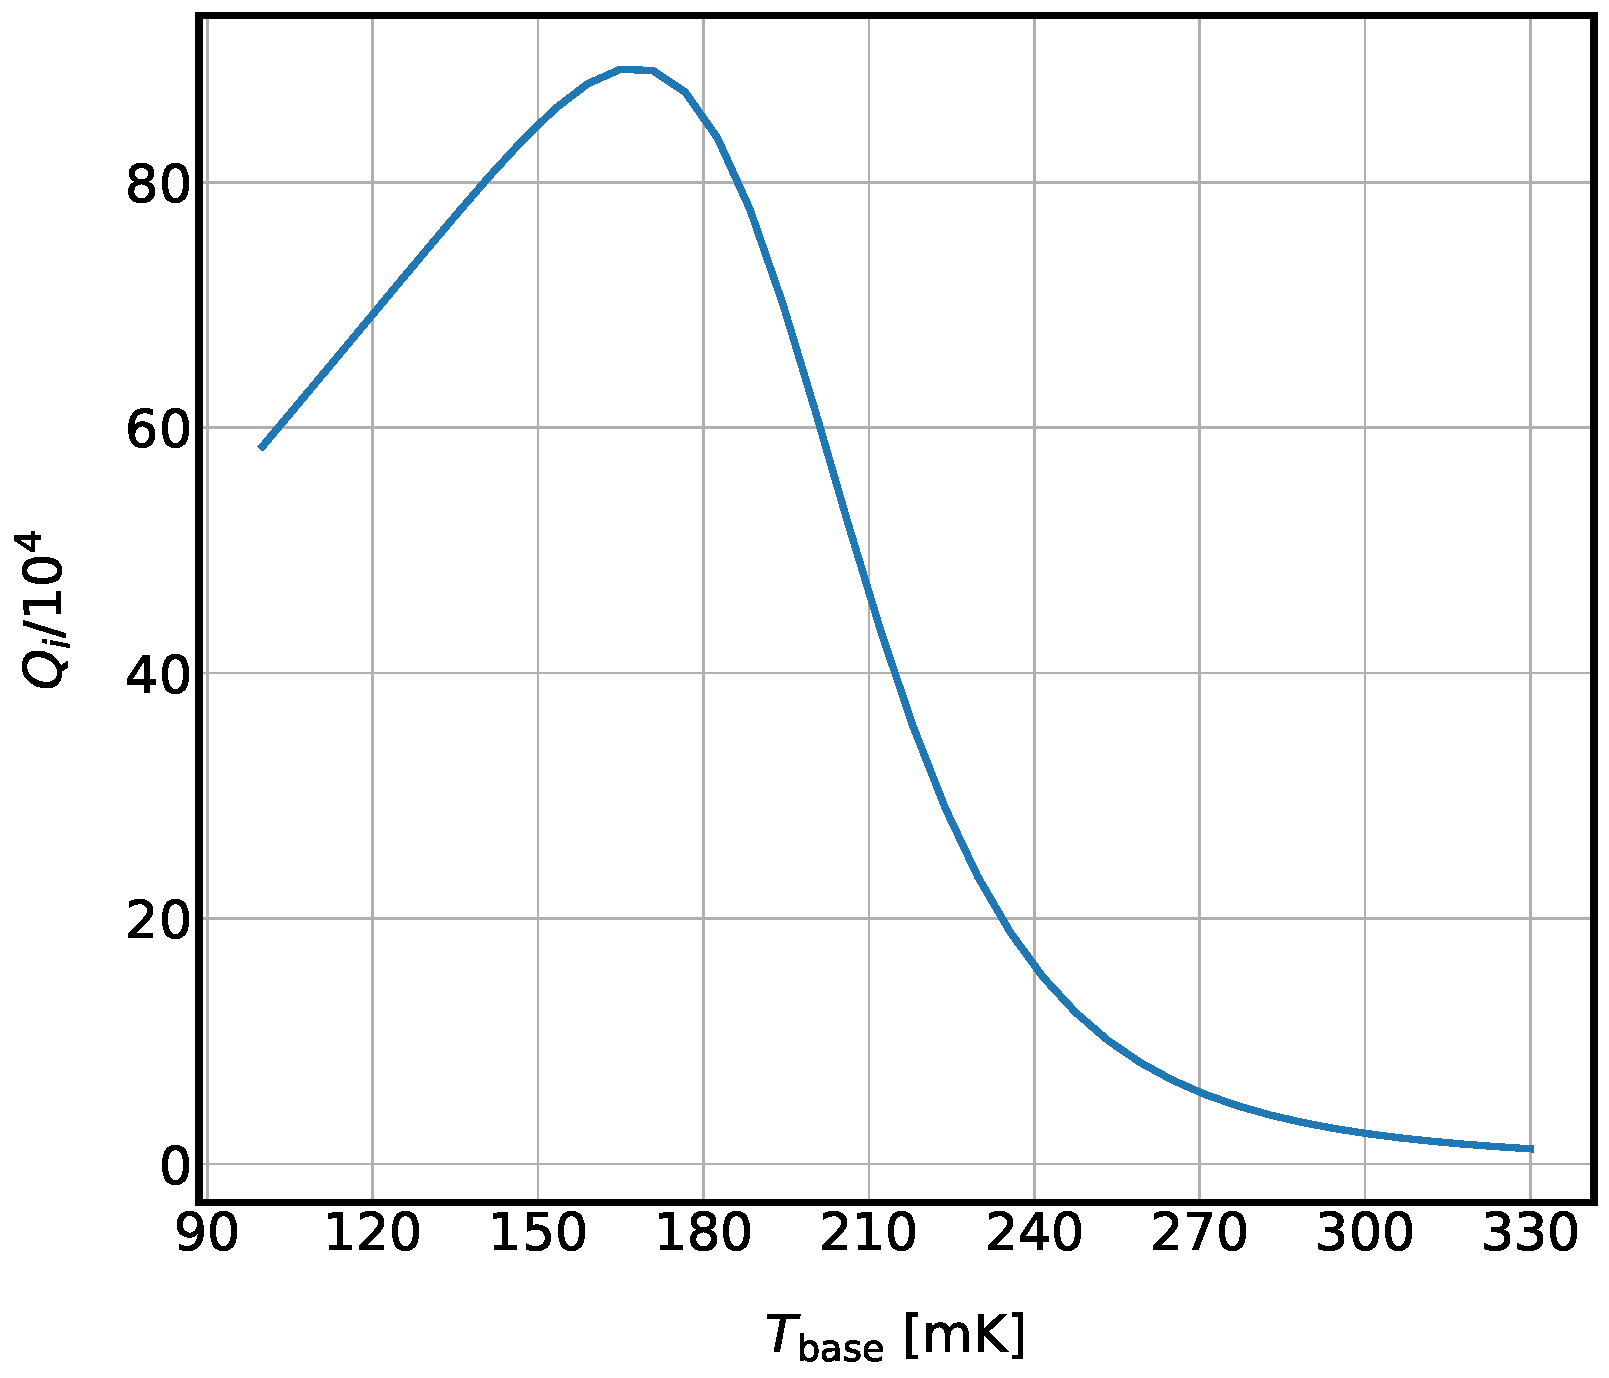
\includegraphics[width=0.8\textwidth]{figures/kid_model/Qi_v_T}
\caption[~Simulated \macrocapwrap{\gls{Qi}} as a function of base temperature.]{Simulated \gls{Qi} as a function of base temperature.}
\label{fig:Qi_T}
\end{figure}

\begin{figure}[!htbp]
\centering
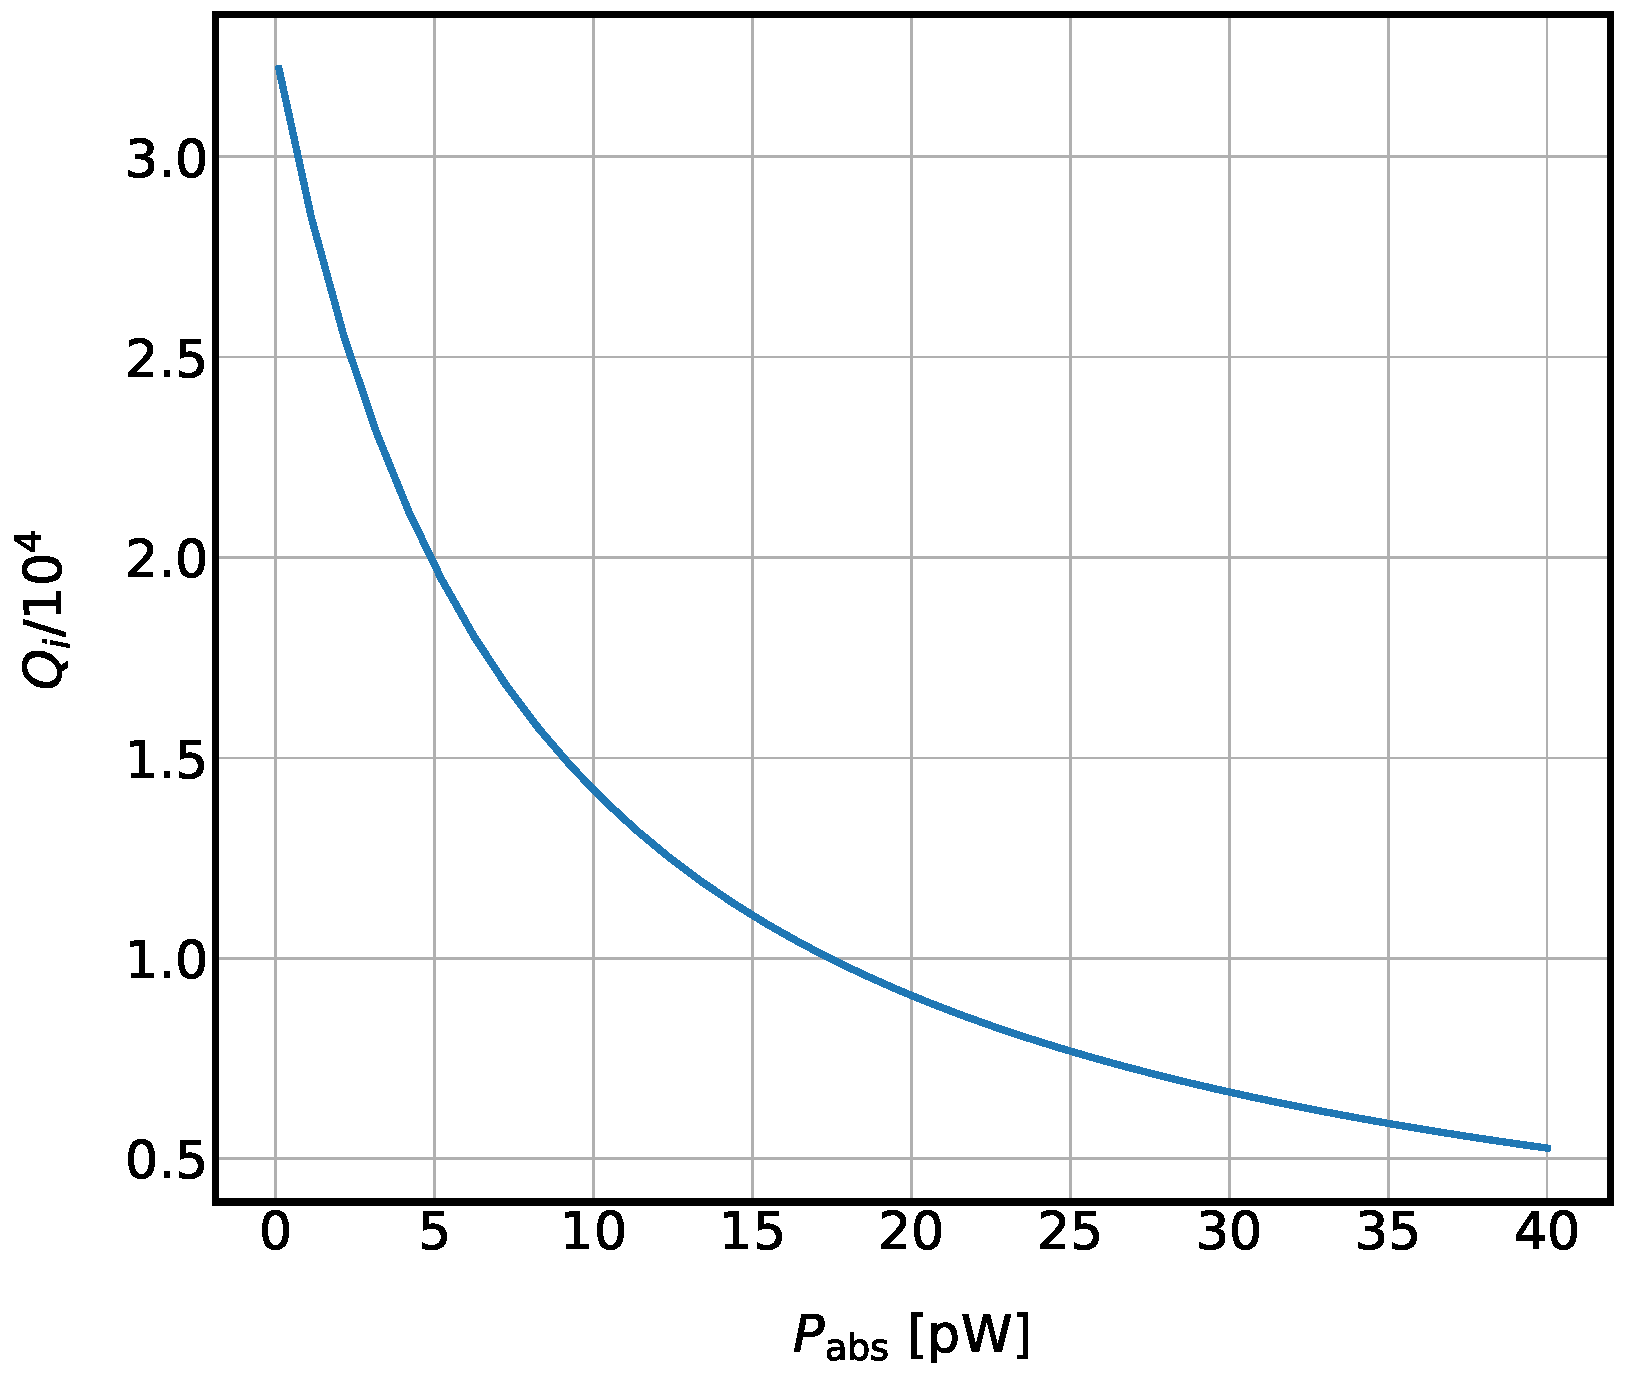
\includegraphics[width=0.8\textwidth]{figures/kid_model/Qi_v_P}
\caption[~Simulated \macrocapwrap{\gls{Qi}} as a function of absorbed optical power.]{Simulated \gls{Qi} as a function of absorbed optical power.}
\label{fig:Qi_P}
\end{figure}
\end{comment}

The empirically determined resonator parameters are determined by measuring the phase and amplitude of the carrier tone after it passes through the LEKID circuit. The resonator impedance  $Z_{r}$ has a frequency dependence which can be expressed as:

\begin{equation}
  Z_{r}(\omega) \simeq Z_{0}\Bigg[ \frac{\gls{Qc}}{2\gls{Qi}} + j\gls{Qc}\delta x \Bigg] \frac{1}{1 + j\gls{asym}}
\end{equation}

where $\delta x = \frac{\omega - \omega_{0}}{\omega_{0}}$. The forward transmission coefficient, $S_{21}$, of the carrier tone expressed as a function of frequency, base temperature and optical power (the dependence of the latter two parameters is implicit) is:

\begin{equation}\label{eq:S21_Z}
  \begin{aligned}
  S_{21}(\omega, T, P) &= 1 - \frac{1}{1 + 2Z_{r}/Z_{0}} \\
                 &= 1 - \frac{1 + j\gls{asym}}{1 + j\gls{asym} \frac{\gls{Qr}}{\gls{Qc}}}\frac{\gls{Qr}}{\gls{Qc}}\Bigg[ \frac{1}{1 + 2j\gls{Qr}\delta x / ( 1 + j\gls{asym}\frac{Qr}{Qc}) }  \Bigg]
  \end{aligned}
\end{equation}

for $\gls{asym} \ll 1$, this reduces to:

\begin{equation}\label{eq:S21}
  S_{21}(\omega, T, P) \simeq 1 - \frac{\gls{Qr}}{\gls{Qc}}\frac{1}{1 + 2j\gls{Qr}\delta x}
\end{equation}

\begin{figure}[!htbp]
  \centering
  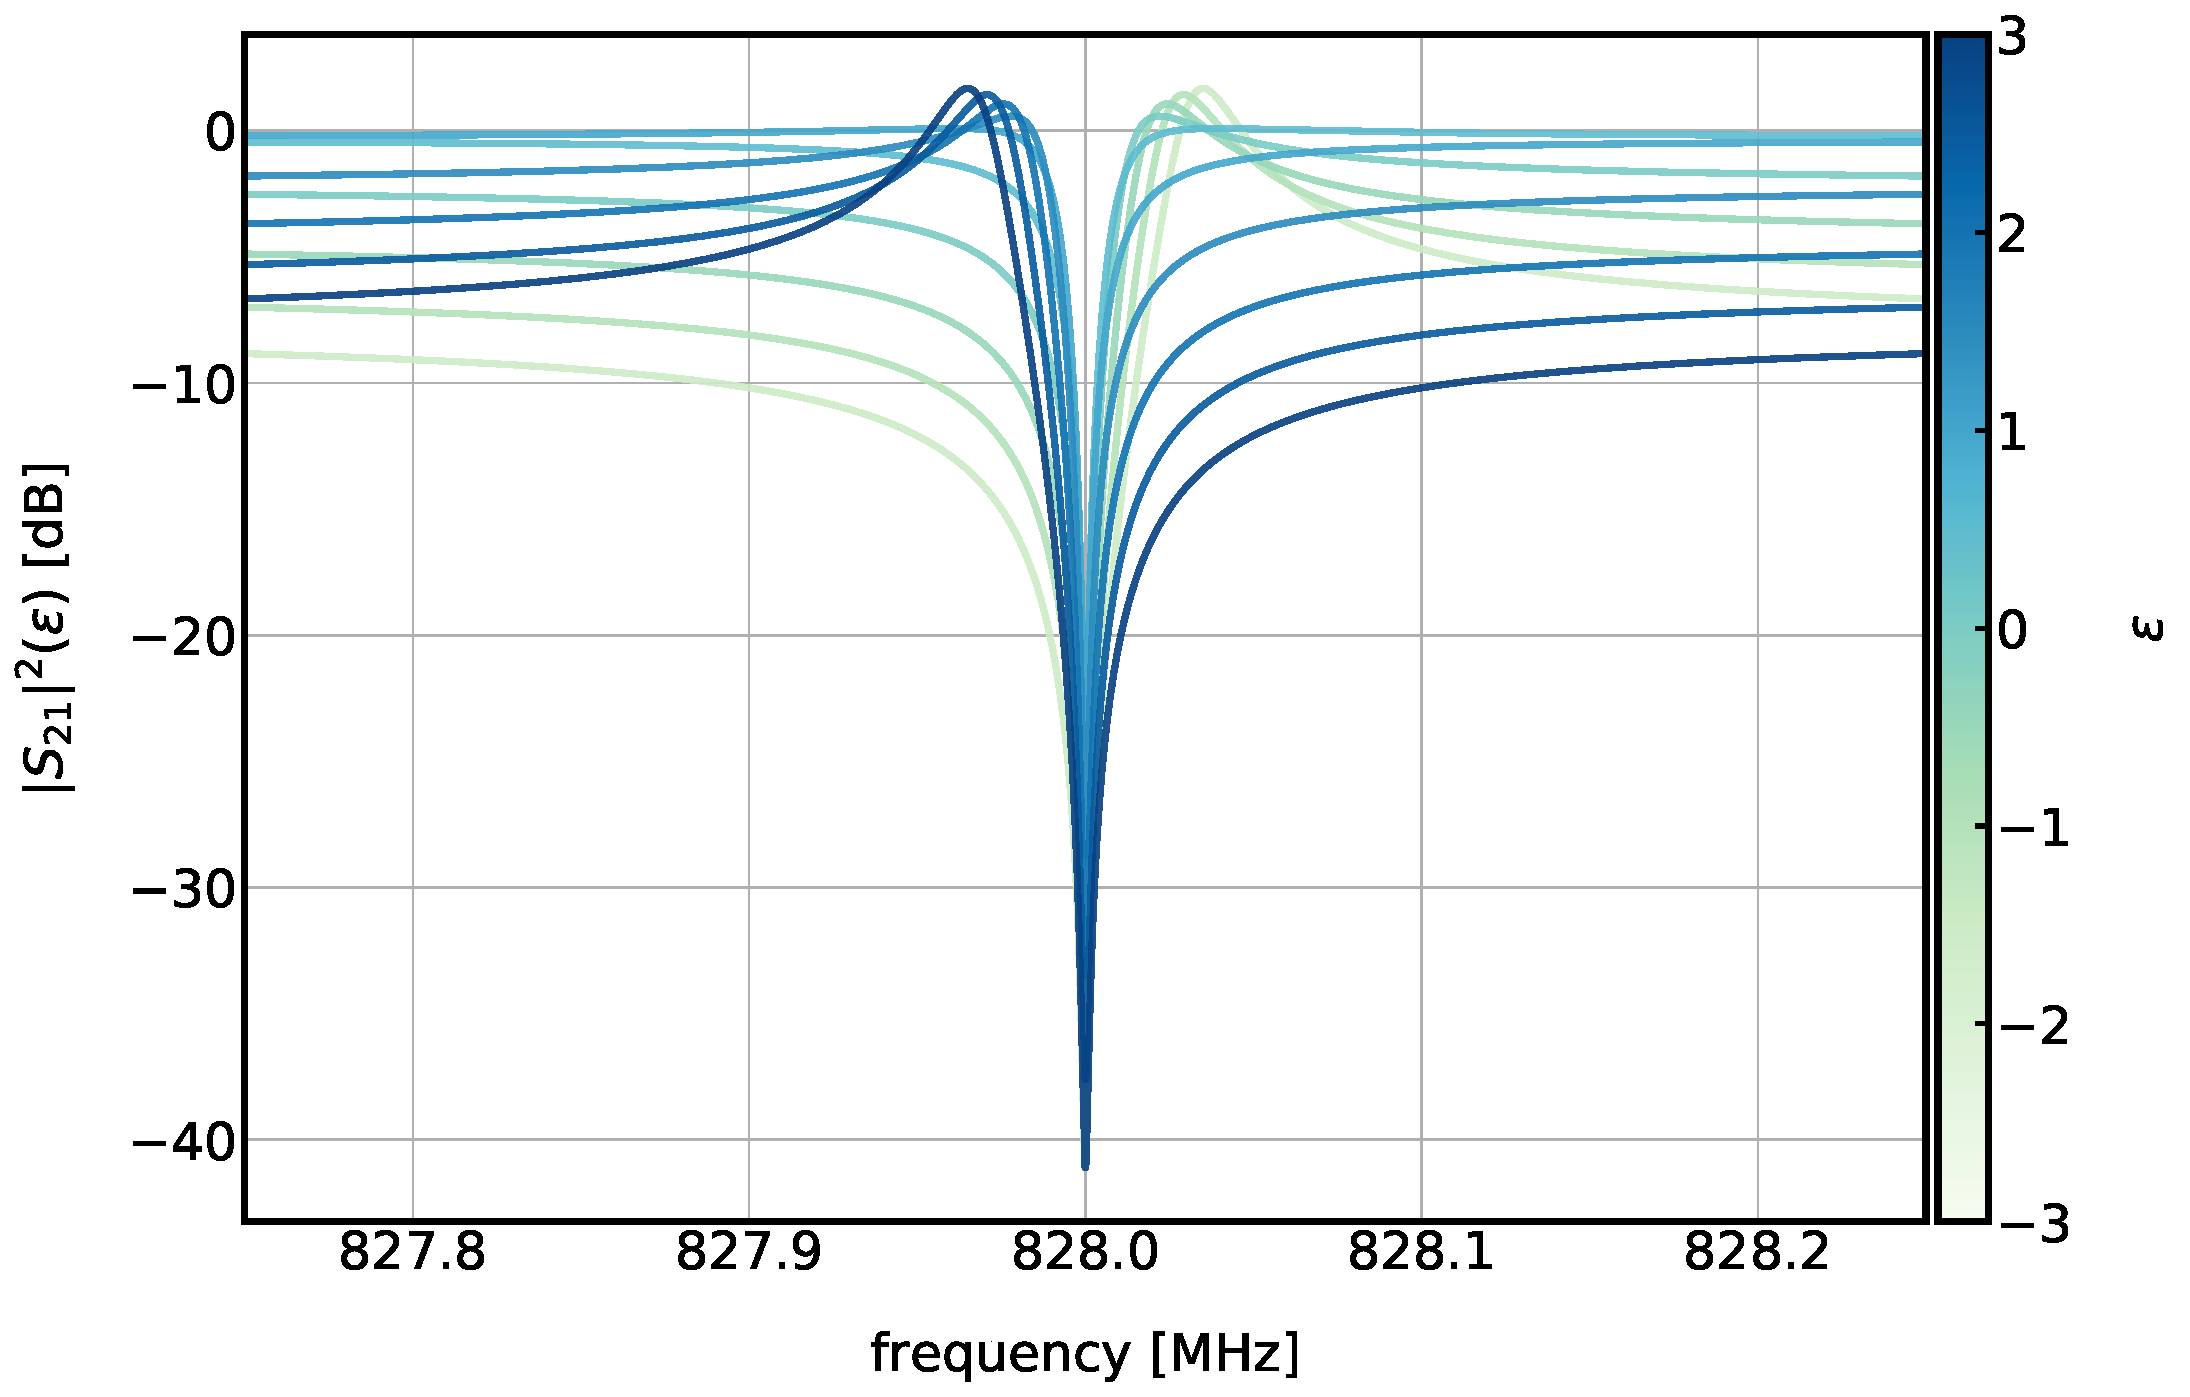
\includegraphics[width=\textwidth]{figures/kid_model/S21_eps}
  \caption[~\macrocapwrap{|\gls{S21}|($\omega$)} for a range of asymmetry parameters.]{$\left| S_{21} \right|(\omega)$ shown for a range of \gls{asym}.}
  \label{fig:S21_eps}
\end{figure}

\begin{figure}[!htbp]
  \centering
  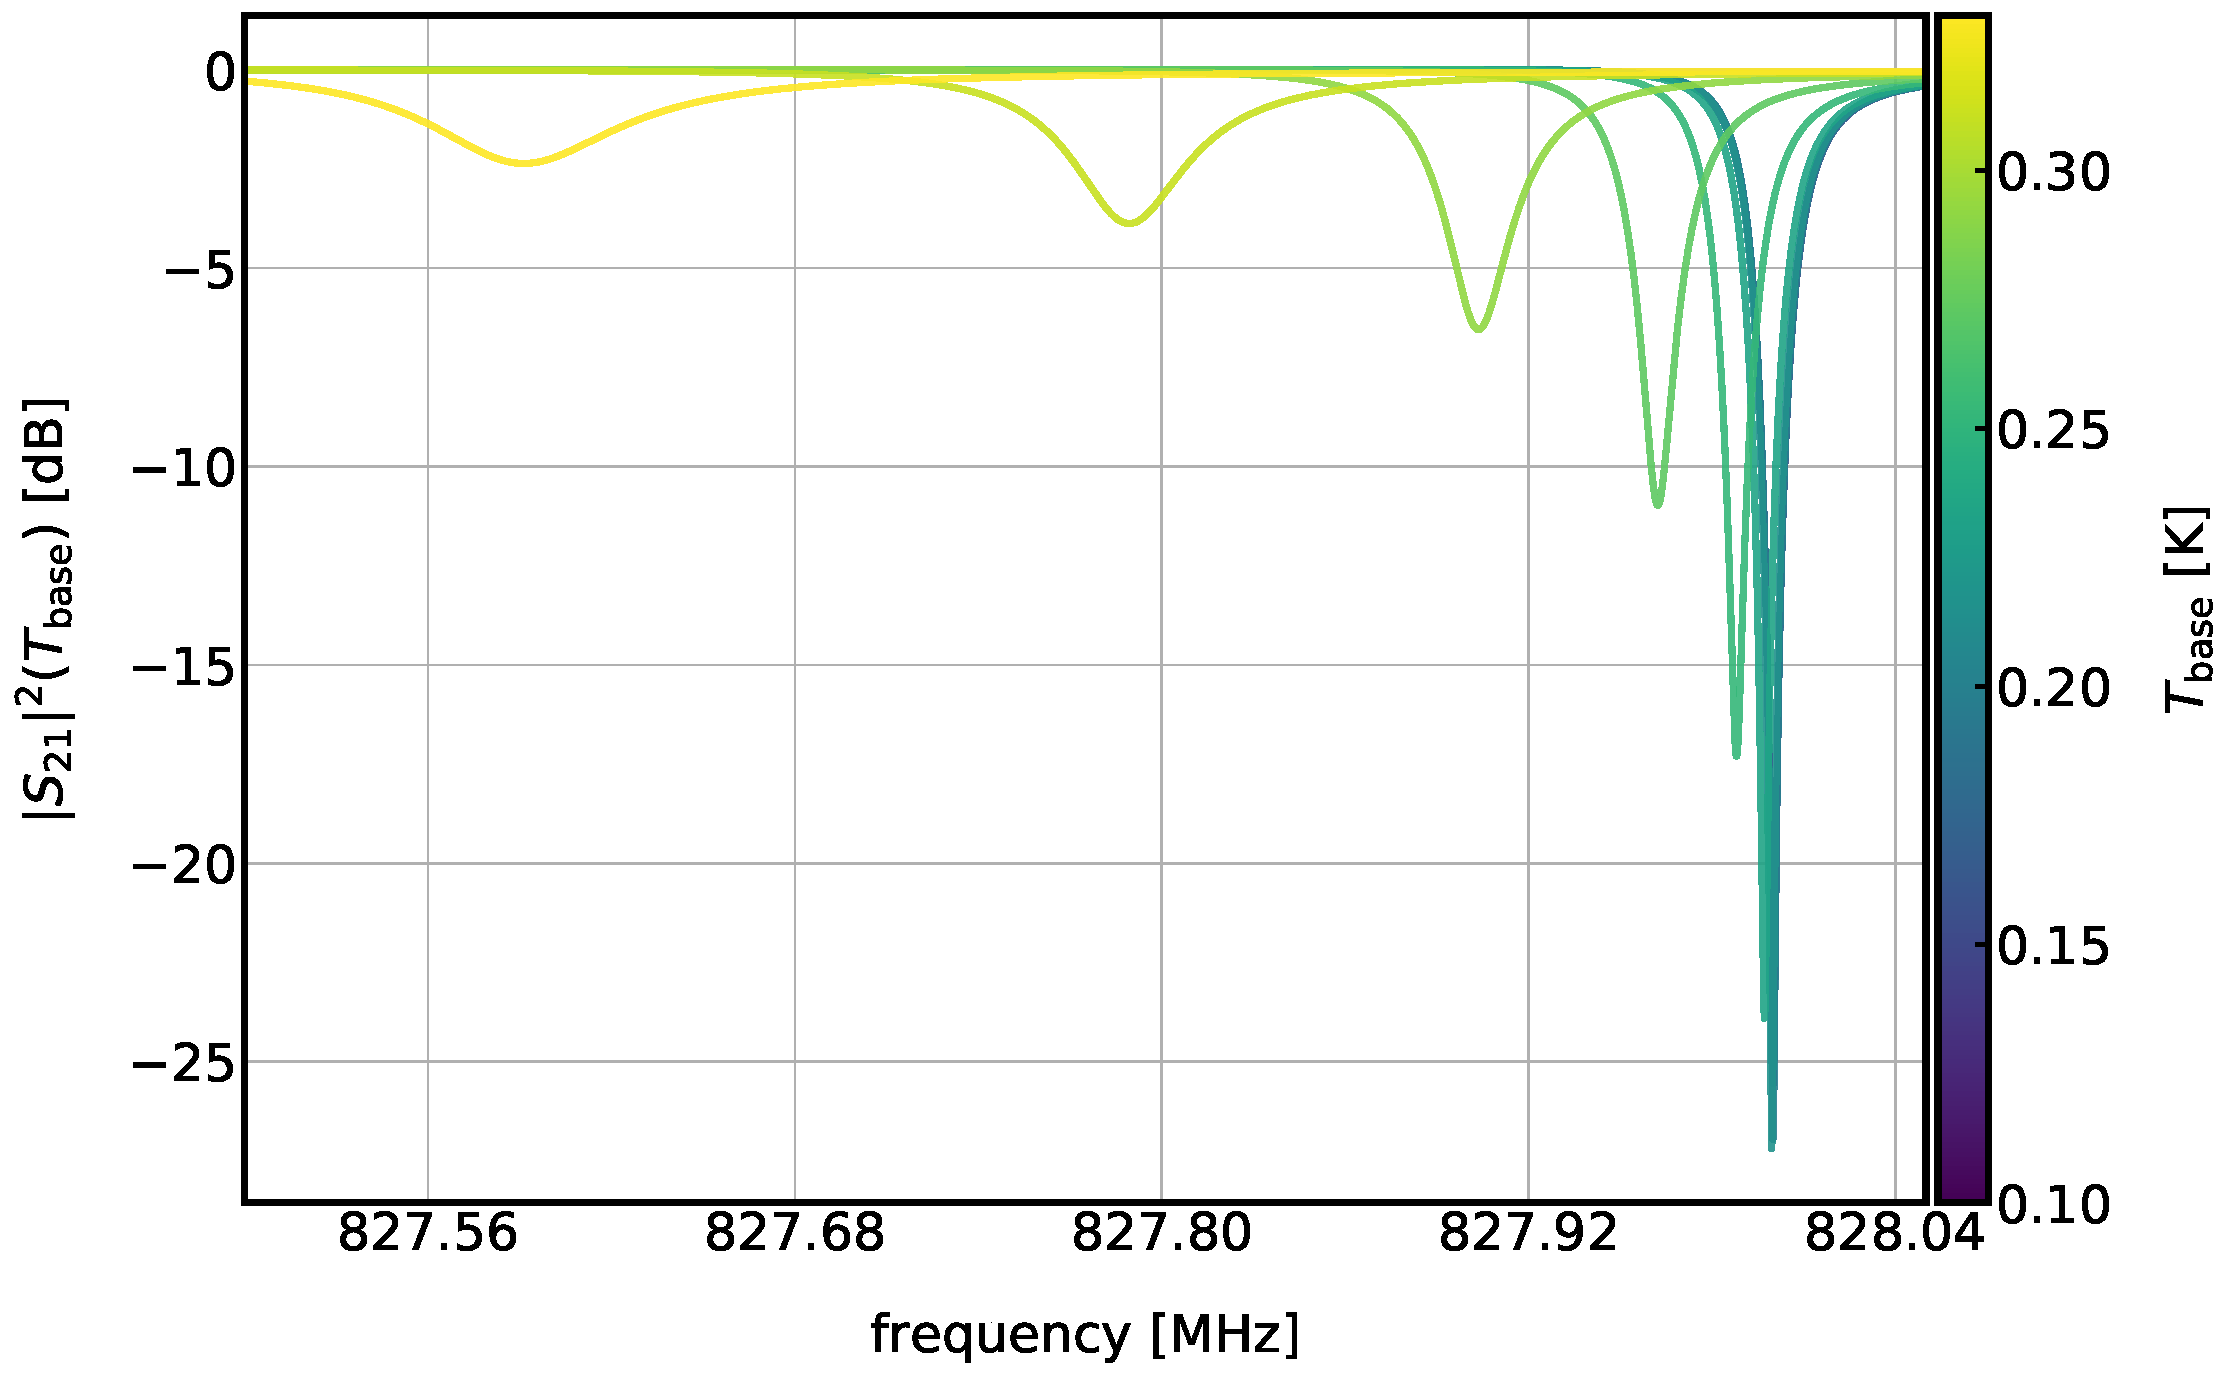
\includegraphics[width=\textwidth]{figures/kid_model/S21_T250}
  \caption[~Simulated \macrocapwrap{|\gls{S21}|($\omega$)} as a function of base temperature.]{Simulated |\gls{S21}|($\omega$) as a function of base temperature.}
  \label{fig:S21_T}
\end{figure}

\begin{figure}[!htbp]
  \centering
  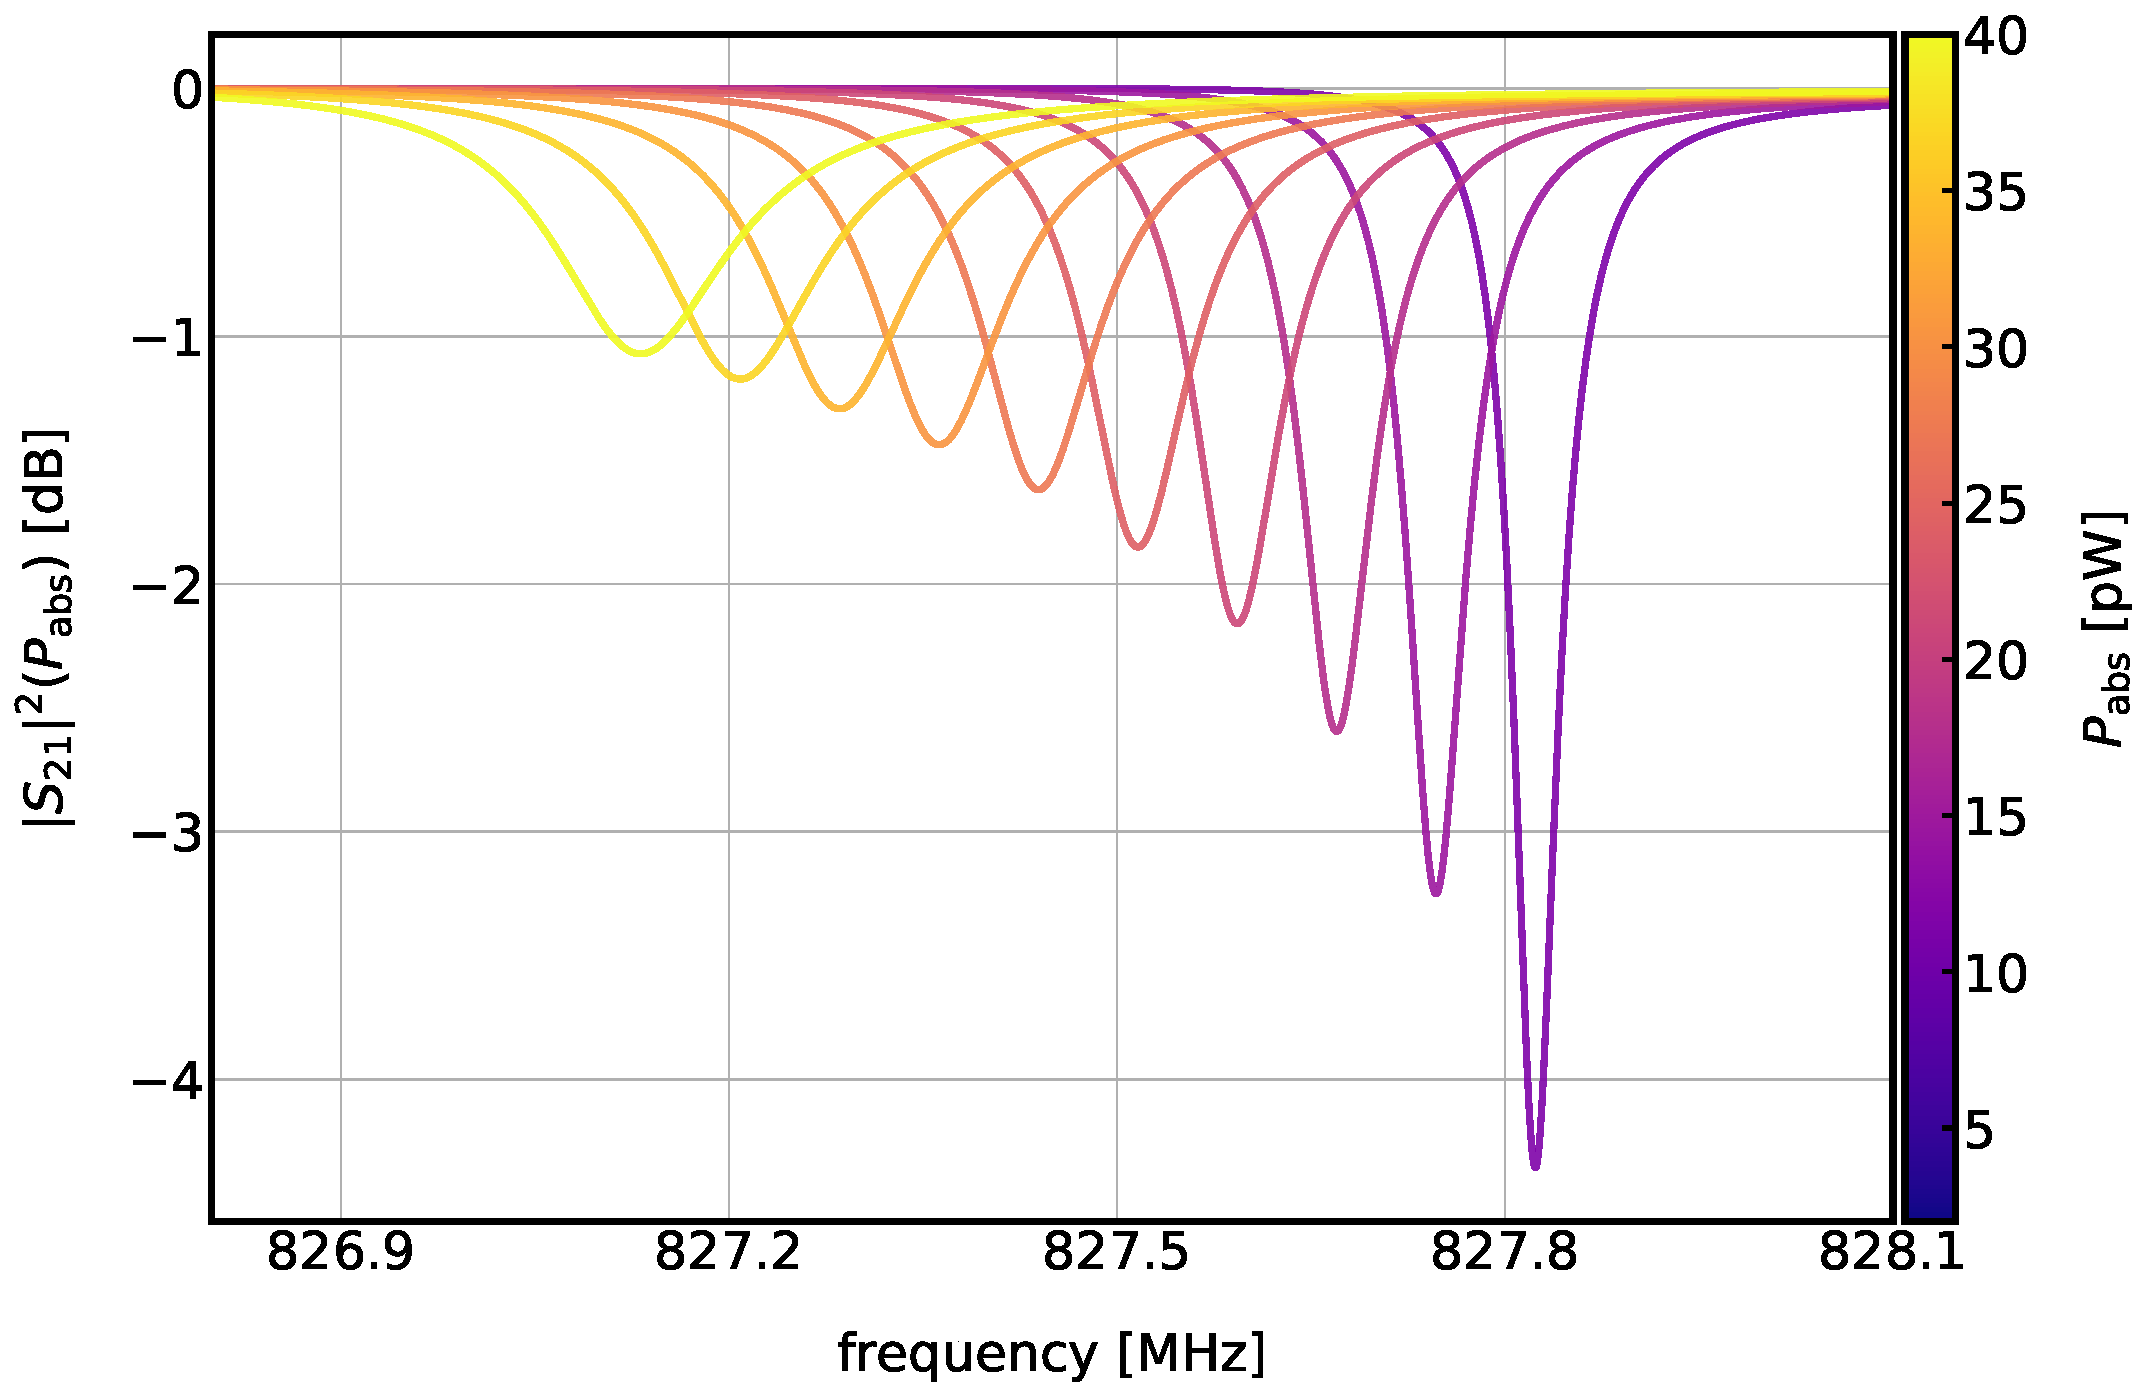
\includegraphics[width=\textwidth]{figures/kid_model/S21_opt250}
  \caption[~Simulated \macrocapwrap{|\gls{S21}|($\omega$)} as a function of optical power.]{Simulated |\gls{S21}|($\omega$) as a function of optical power.}
  \label{fig:S21_opt}
\end{figure}

\begin{figure}[!htbp]
  \centering
  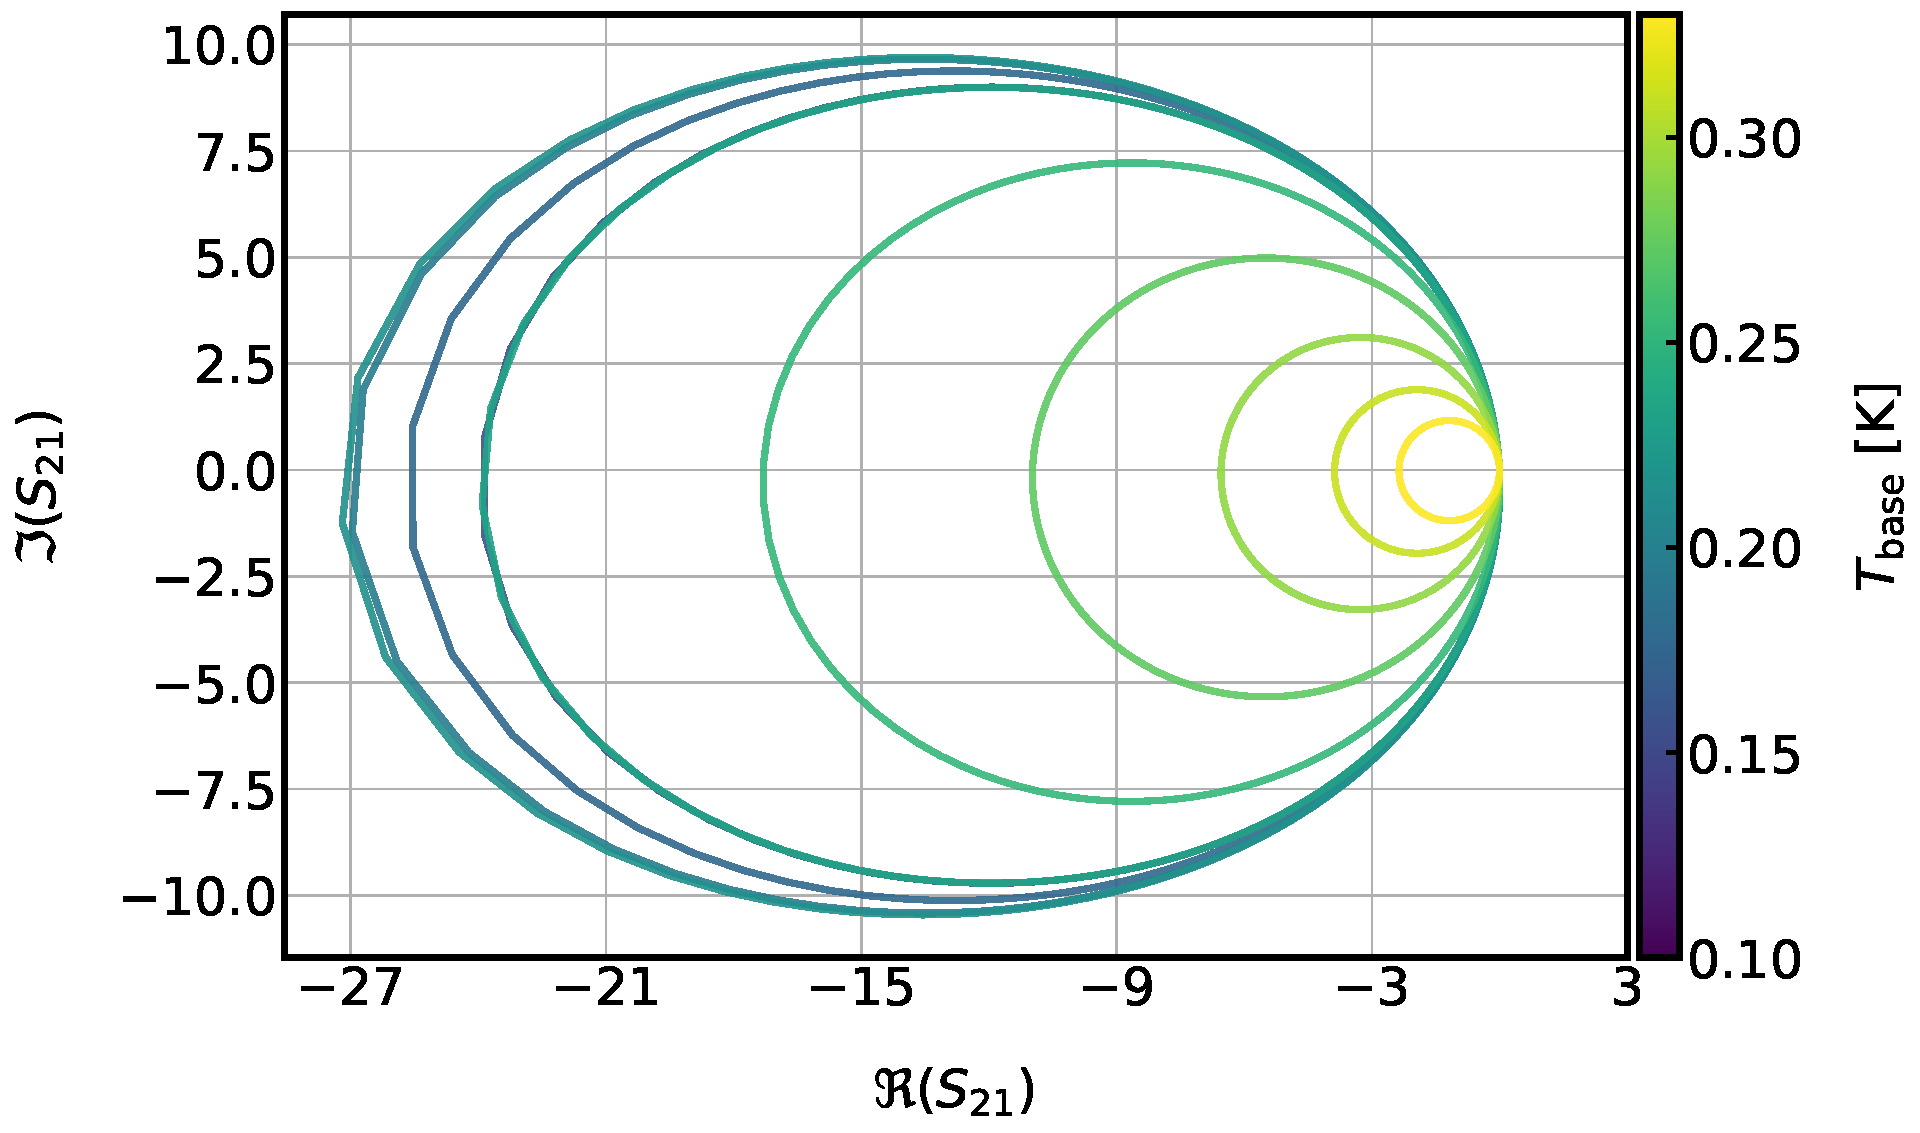
\includegraphics[width=\textwidth]{figures/kid_model/IQloop_T250}
  \caption[~The simulated \macrocapwrap{$I/Q$} loop as a function of base temperature.]{The simulated $I/Q$ loop as a function of base temperature.}
  \label{fig:IQloop_T}
\end{figure}

\begin{figure}[!htbp]
  \centering
  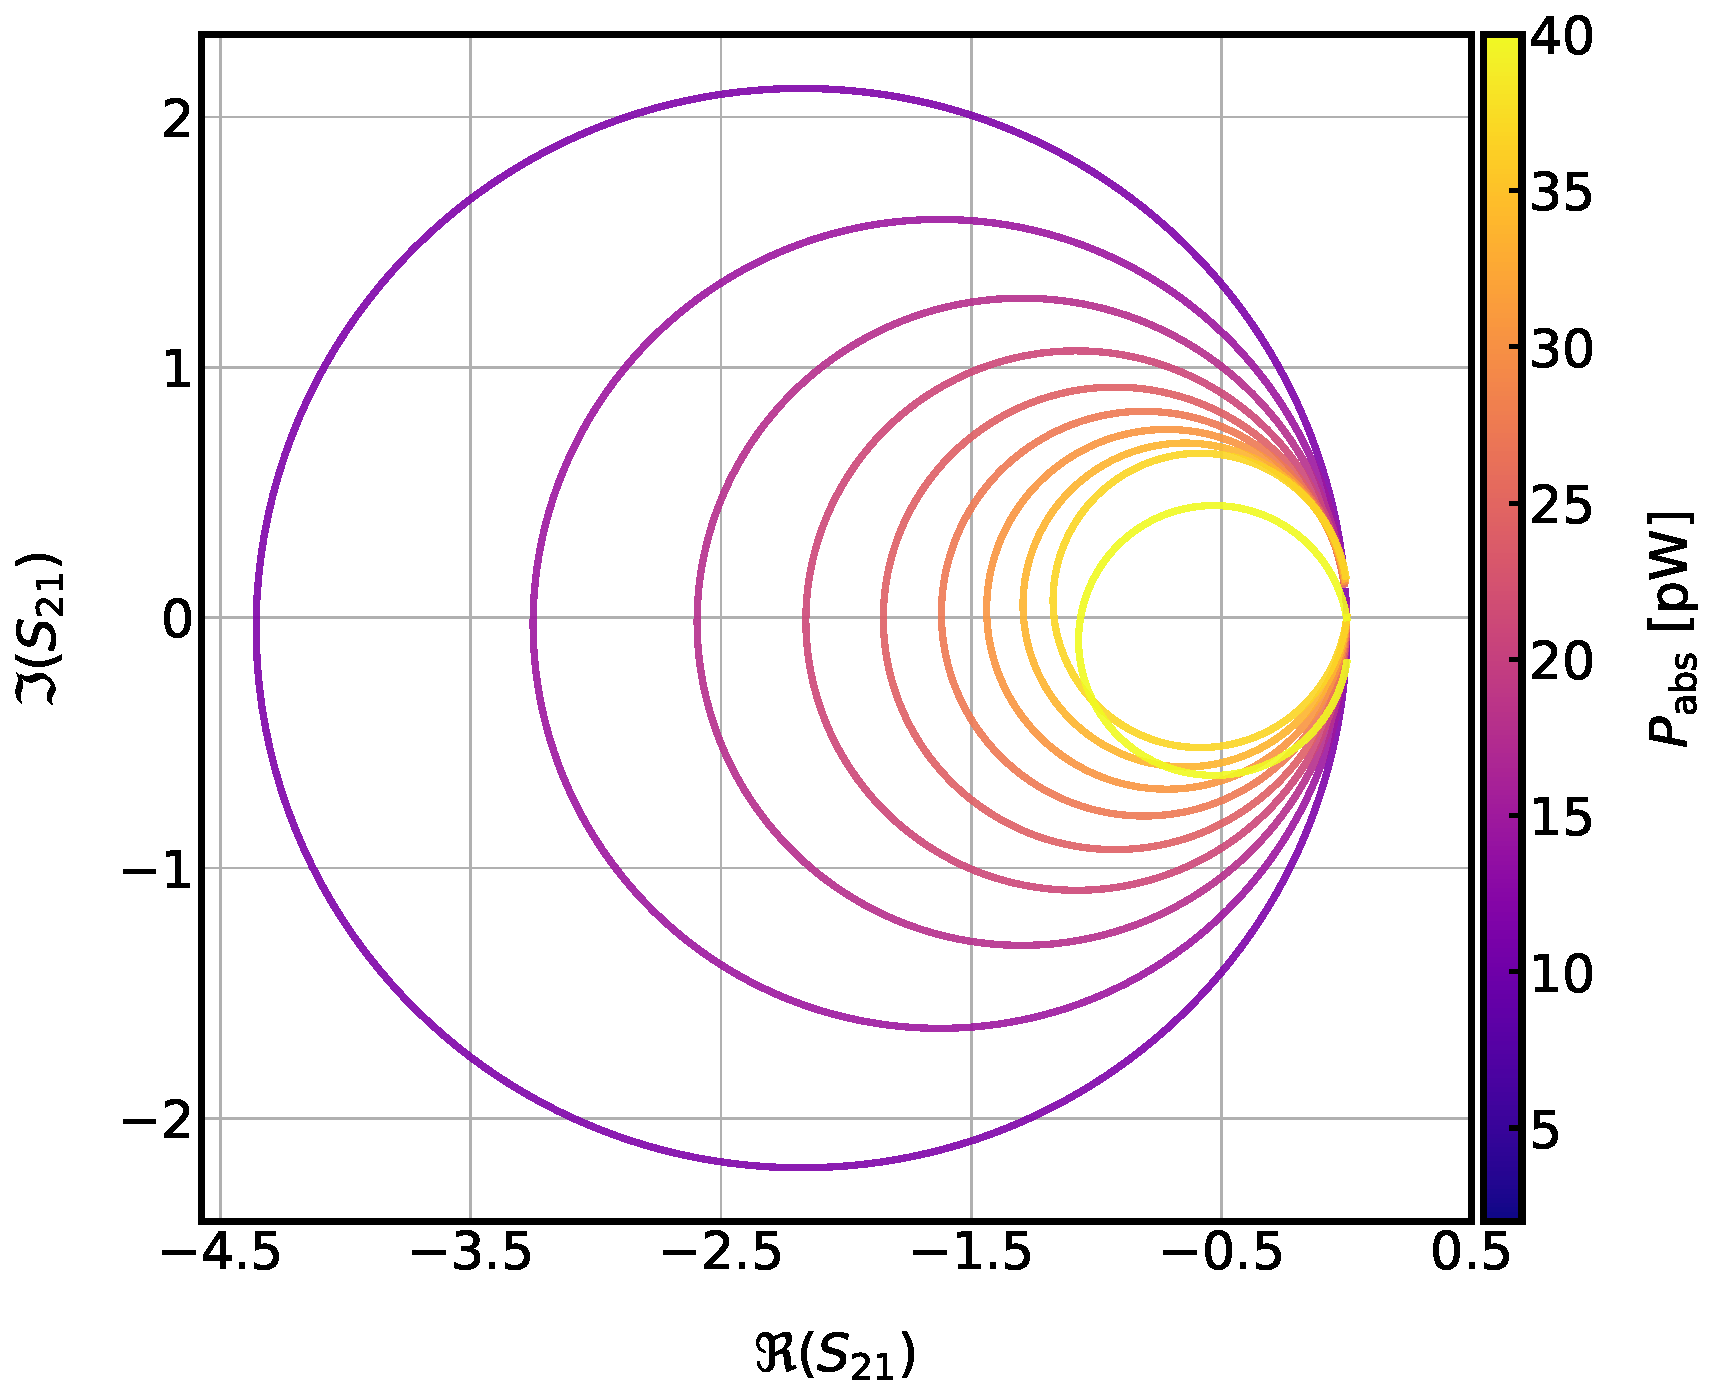
\includegraphics[width=\textwidth]{figures/kid_model/IQloop_opt250}
  \caption[~The simulated \macrocapwrap{$I/Q$} loop as a function of optical power.]{The $I/Q$ loop as a function of optical power.}
  \label{fig:IQloop_P}
\end{figure}

Figure~\ref{fig:S21_eps} shows an example $\left| S_{21} \right|(\omega)$ for a wide range (-3--+3) of \gls{asym} values. The temperature and power dependence of \gls{S21} are shown in Figures~\ref{fig:S21_T} and \ref{fig:S21_opt}, for a simulated BLAST-TNG 250~$\upmu$m resonator with $\omega_{0} = 828$~MHz. The `dip-depth' of the \gls{S21} traces is a function of the quality factors:

% dip depth
\begin{equation}\label{eq:dip_depth}
  D = 20\log_{10}\left( 1 - \frac{\gls{Qr}}{\gls{Qc}}\right)
\end{equation}

The `$I/Q$' loops corresponding to Figures~\ref{fig:S21_T} and \ref{fig:S21_opt} are shown in Figures~\ref{fig:IQloop_T} and \ref{fig:IQloop_P}, where $I = \Re(\gls{S21})$ and $Q = \Im(\gls{S21})$.

\section{Responsivities}\label{sec:responsivity}

In this section, we derive the LEKID responsivity to fluctuations in base temperature \gls{Tbase} and absorbed optical power \gls{Pabs}.

\subsection{Temperature Responsivity}

The change in the LEKID's resonant frequency in response to a change in base temperature can be written as:

\begin{equation}\label{eq:RT}
  \begin{aligned}
  \gls{Rtemp} &= \frac{df_{0}}{dT} \\
              &= \frac{df_{0}}{d\gls{sig2}} \frac{d\gls{sig2}}{d\gls{nqp}} \frac{d\gls{nqp}}{dT}
  \end{aligned}
\end{equation}

where:

\begin{equation}\label{eq:df0_dsig2}
  \frac{df_{0}}{d\gls{sig2}} = \frac{\alpha f_{0}}{2\gls{sig2}}
\end{equation}

and for $\gls{Tbase} \ll \gls{Tc}$,

\begin{equation}\label{eq:dnqp_dT}
  \frac{d\gls{nqp}}{dT} \simeq \frac{\gls{nqp}}{T} \left(\frac{1}{2} + \frac{\gls{Delta}}{kT} \right)
\end{equation}

Derivations of Equations~\ref{eq:df0_dsig2} and~\ref{eq:dnqp_dT} can be found in \citet{mauskopf2018transition}.

Equation~\ref{eq:RT} is shown graphically in Figure~\ref{fig:dfdT}. It can be seen that \gls{Rtemp} decreases monotonically with increasing \gls{Tbase}.

\begin{figure}[!htbp]
\centering
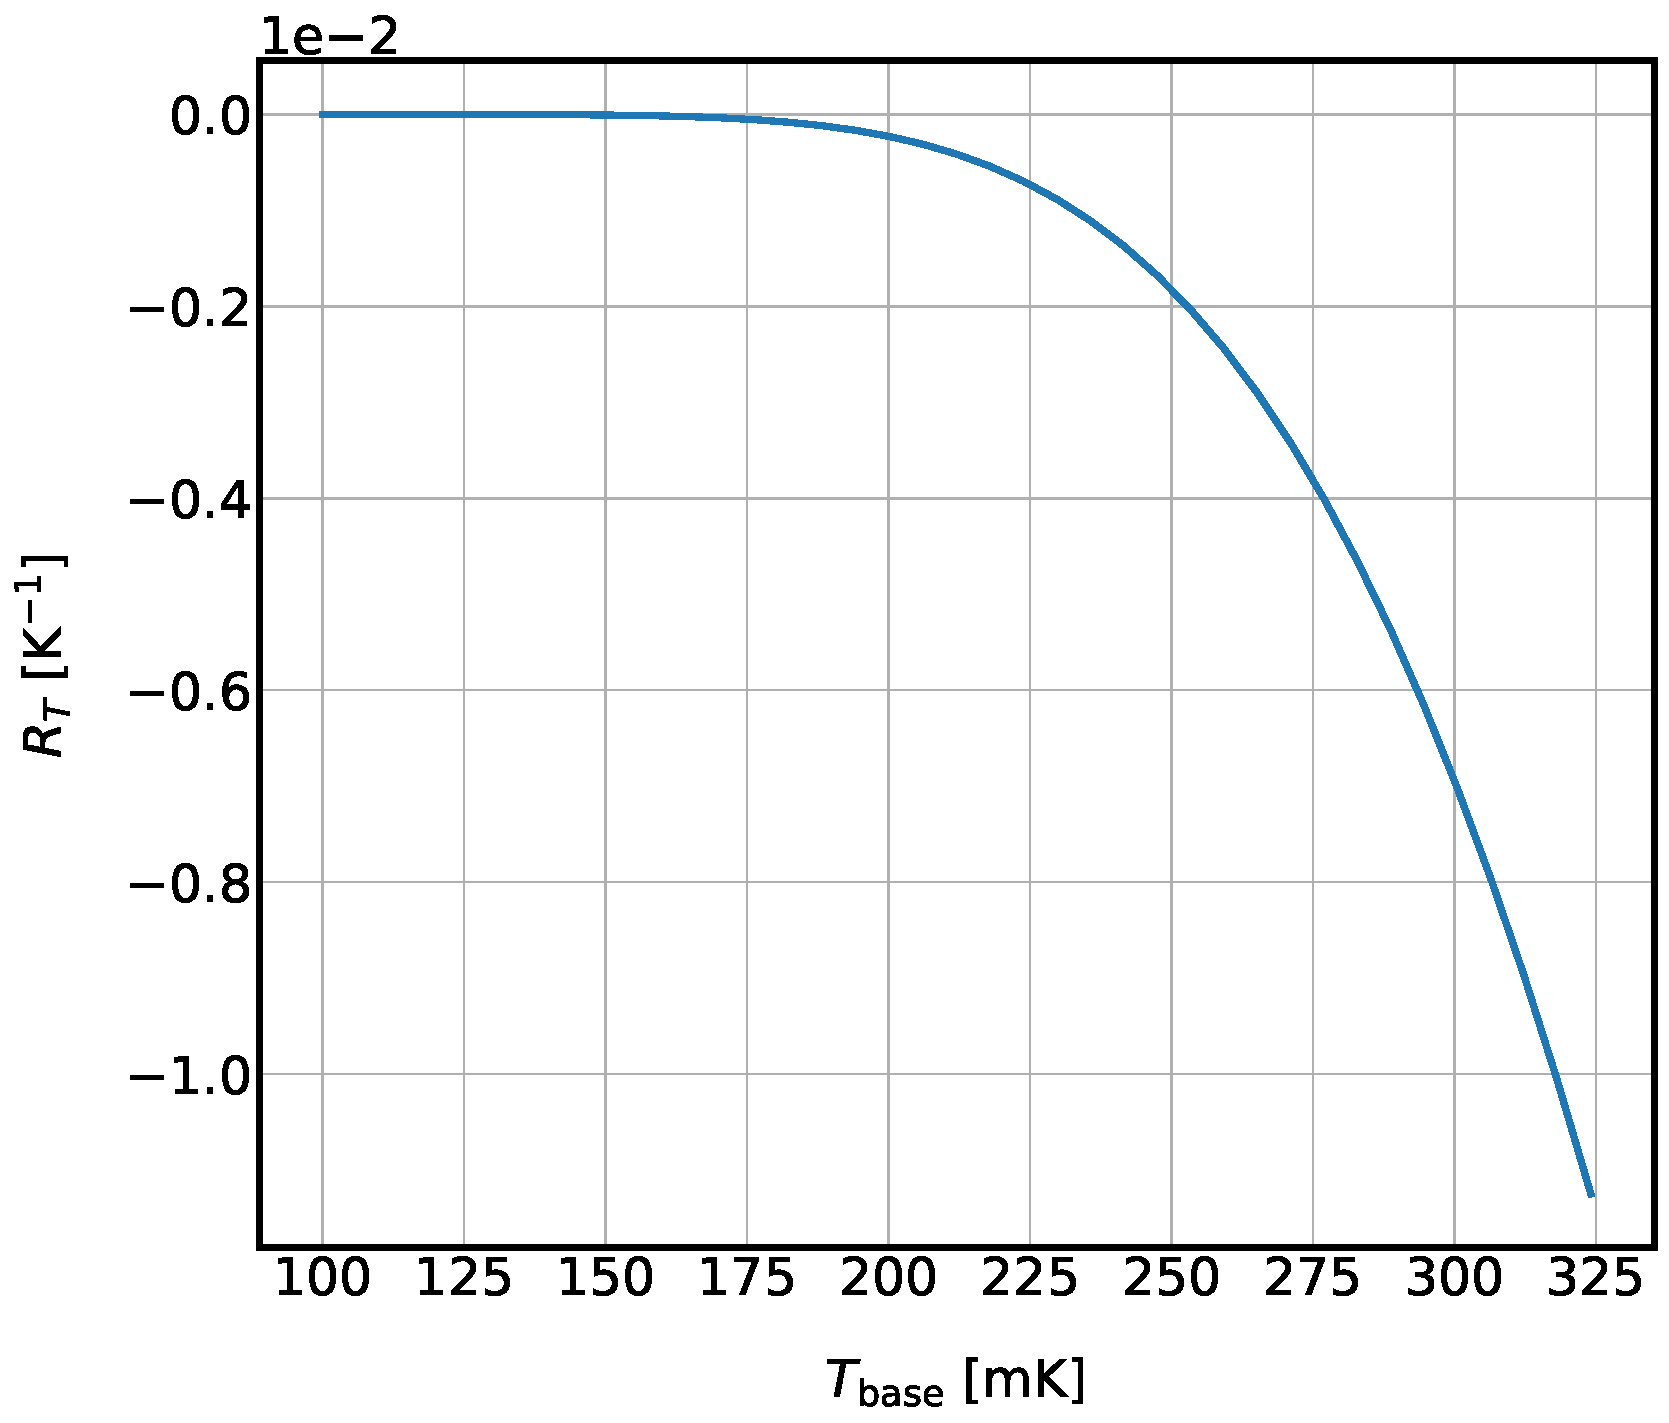
\includegraphics[width=0.8\textwidth]{figures/kid_model/dfdT}
\caption[~Simulated LEKID temperature responsivity.]{Simulated LEKID temperature responsivity \gls{Rtemp}.}
\label{fig:dfdT}
\end{figure}

\subsection{Optical Responsivity}

At a fixed base temperature, the change in the LEKID's resonant frequency in response to a change in absorbed optical power can be written as:

\begin{equation}
    R_{P} = \frac{df_{0}}{d\gls{Pabs}} = \frac{df_{0}}{d\gls{sig2}} \frac{d\gls{sig2}}{d\gls{nqp}} \frac{d\gls{nqp}}{d\gls{Pabs}}
\end{equation}

where:

\begin{equation}
  \frac{df_{0}}{d\gls{sig2}}\frac{d\gls{sig2}}{d\gls{nqp}} \simeq -\frac{\alpha f_{0}} {4\gls{N0}\gls{Delta}} \left( 1 + \sqrt{ \frac{2 \Delta_{0}}{\pi K T}} \right)
\end{equation}

The expression for $\frac{d\gls{nqp}}{d\gls{Pabs}}$ is case dependent. Here, we provide a brief overview of three cases, as found in \citet{mauskopf2018transition}. We first consider the rate of change in the total number density of QP:

\begin{equation}\label{eq:dn_dt}
  \begin{aligned}
  \frac{\gls{nqp}}{dt} &= \Gamma_{opt} + \Gamma_{ro} + \Gamma_{therm} + \Gamma_{rec} \\
   &= \frac{\gls{det_eff} \gls{Pabs}}{\Delta \Sigma} + \frac{\epsilon_{ro} P_{ro}}{\Delta \Sigma} + \gamma \gls{N0}^{2} 8\pi k T \Delta e^{-2 \Delta / kT} -\frac{\gls{nqp}}{\gls{tau_qp}}
  \end{aligned}
\end{equation}

where:
\begin{itemize}[label={},nosep]
  \item $\Gamma_{opt}$ is the QP generation rate due to absorbed optical power.
  \item $\Gamma_{ro}$ is the QP generation rate due to microwave readout power.
  \item $\Gamma_{therm}$ is the QP generation rate due to thermal phonons.
  \item $\Gamma_{rec}$ is the QP recombination rate into CPs.
  \item \gls{det_eff} is the efficiency of QP generation from absorbed optical power.
  \item $\epsilon_{ro}$ is the internal QP generation efficiency for absorbed readout power.
  \item $\gamma = 1/(\gls{nqp}\gls{tau_qp})$ is a constant relating the number density of QP to the QP recombination time.
\end{itemize}

In the first case (\textit{Case 1}), we assume that QP generation is dominated by the absorption of photons. Equation~\ref{eq:dn_dt} then becomes

% case 1

\begin{equation}
    \frac{\gls{nqp}}{dt} \simeq \frac{\gls{det_eff} \gls{Pabs}}{\Delta \Sigma} - \gamma\gls{nqp}^{2}
\end{equation}

Then, $\frac{d\gls{nqp}}{dP\gls{Pabs}}$ can be shown to be:

\begin{equation}\label{eq:case1}
  \frac{d\gls{nqp}}{d\gls{Pabs}} = \frac{1}{2}\sqrt\frac{\eta}{\gamma \gls{Pabs}\Delta\Sigma} = \frac{n_{0}}{2\gls{Pabs}} \frac{1}{1 + j\omega\gls{tau_qp}/2}
\end{equation}

Behavior corresponding to \textit{Case 1} has been observed in Al KIDs (e.g., \citet{de2014quasiparticle,flanigan2016photon,mauskopf2014photon}).

The second case to consider \textit{Case 2} is if the QP generation rate is dominated by thermal phonon` generation, or has a recombination time that does not depend on \gls{Pabs}. In this case, Equation~\ref{eq:dn_dt} becomes:
% case 2

\begin{equation}
    \frac{\gls{nqp}}{dt} \simeq \frac{\gls{det_eff} \gls{Pabs}}{\Delta \Sigma} + \Gamma_{therm} - \frac{\gls{nqp}}{\tau_{\mathrm{eff}}}
\end{equation}

and

\begin{equation}\label{eq:case2}
\frac{d\gls{nqp}}{d\gls{Pabs}} \simeq \frac{\eta\tau_{\mathrm{eff}}}{\Delta\Sigma}\frac{1}{1 + j\omega\tau_{\mathrm{eff}}}
\end{equation}

Behavior corresponding to \textit{Case 2} has been observed in TiN KIDs (e.g., \citet{catalano2014performance,hubmayr2015photon,hailey2016low}).

% intermediate case
In the intermediate case, there is an effective `dark' power loading on the device, $P_{\mathrm{dark}}$, which generates a constant background of QP whose rate of creation is independent of absorbed optical power. In this case,

\begin{equation}
    \frac{\epsilon_{ro} P_{ro}}{\Delta \Sigma} + \gamma \gls{N0}^{2} 8\pi k T \Delta e^{-2 \Delta / kT} - \gamma\gls{nqp}^{2}
\end{equation}

and

\begin{equation}
  \frac{d\gls{nqp}}{dP_{\mathrm{abs}}} = \sqrt{\frac{\gls{det_eff}}{\Delta \Sigma \gamma}}\frac{1}{\sqrt{P_{\mathrm{dark}} + \gls{Pabs}}}
\end{equation}

\begin{figure}[!htbp]
\centering
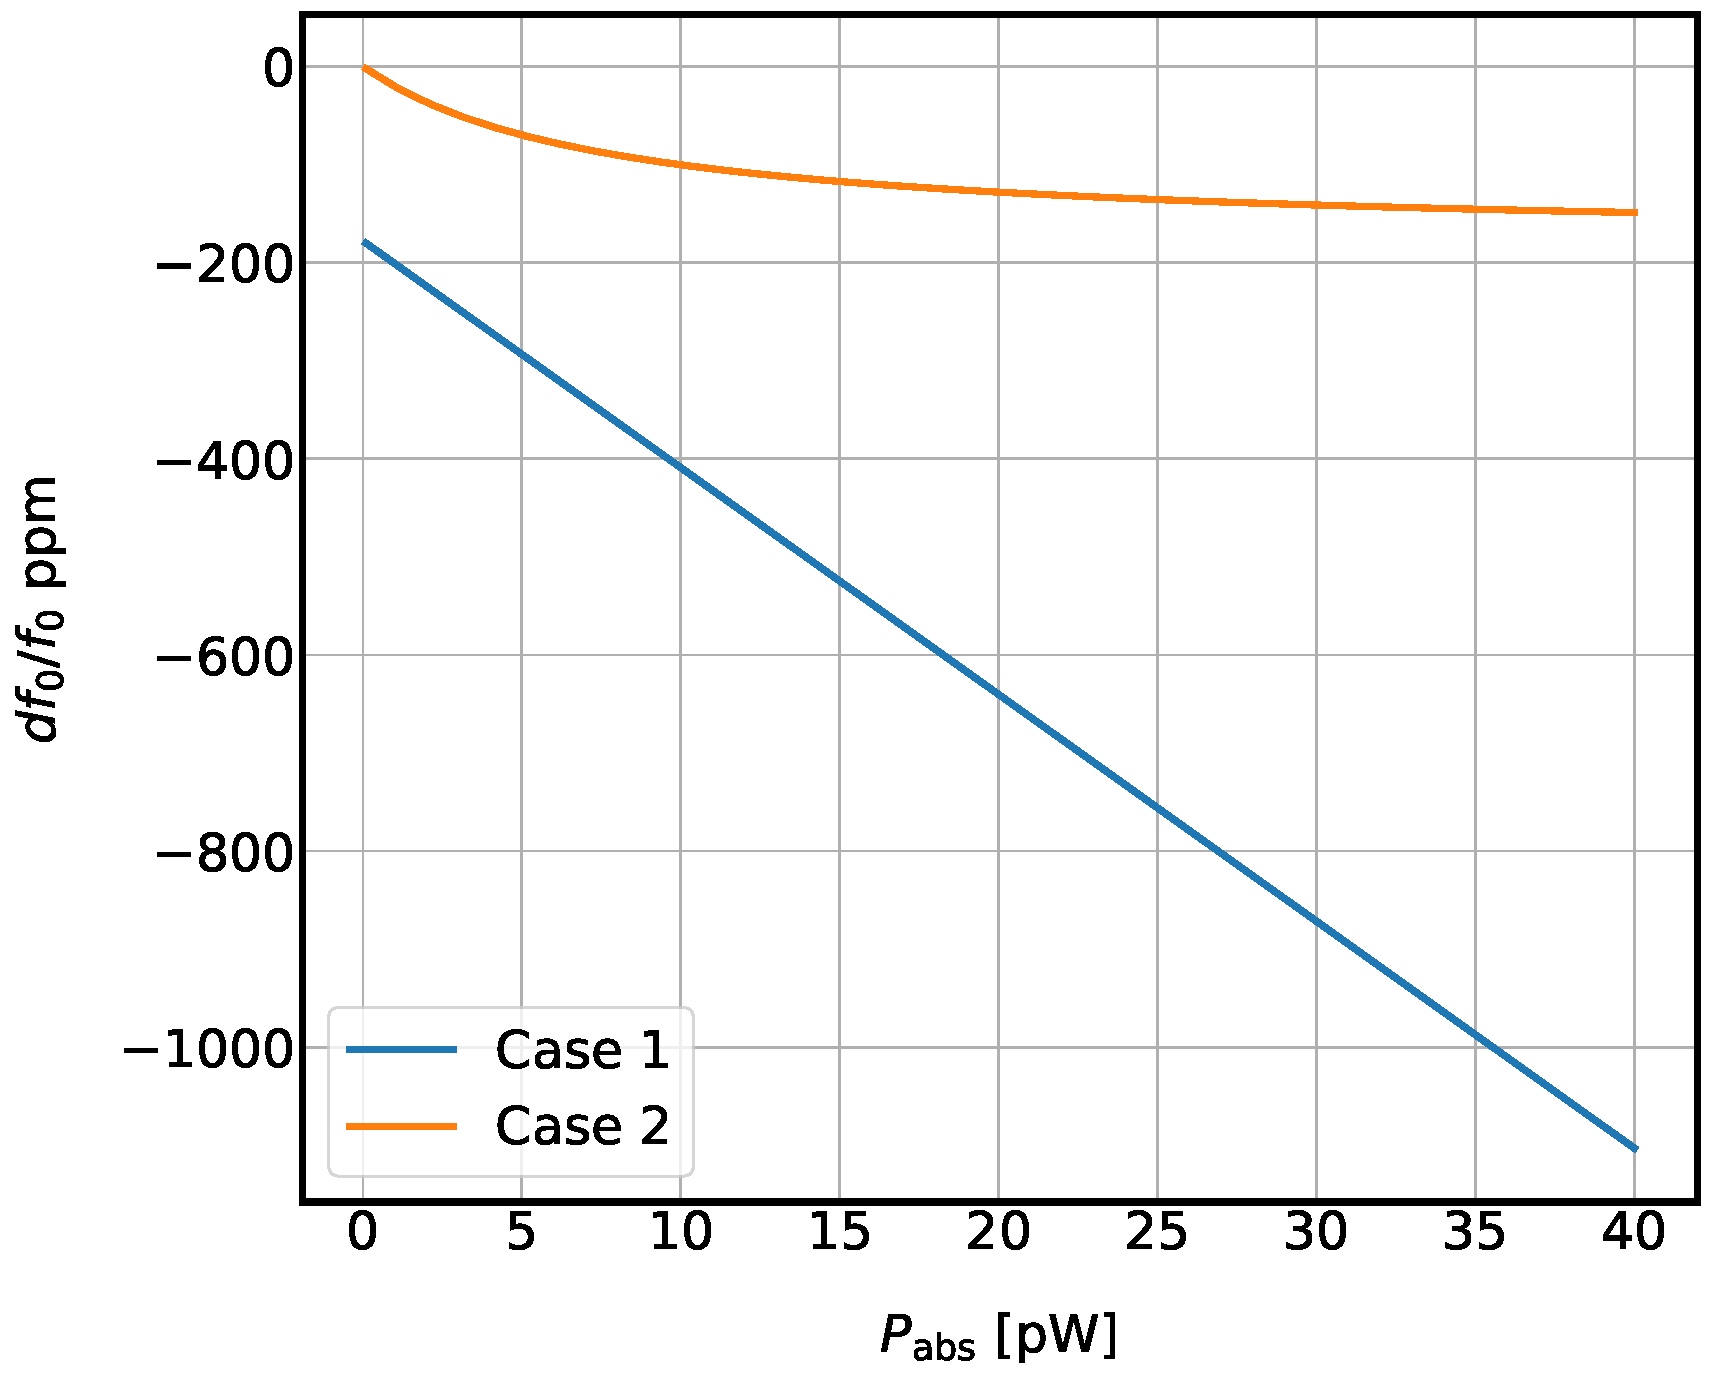
\includegraphics[width=0.8\textwidth]{figures/kid_model/resp_case1_case2}
\caption[~A model of the case~1 and case~2 optical responsivities.]{A model of the \textit{Case 1} and \textit{Case 2} optical responsivities.}
\label{fig:responsivity}
\end{figure}

\begin{figure}[!htbp]
\centering
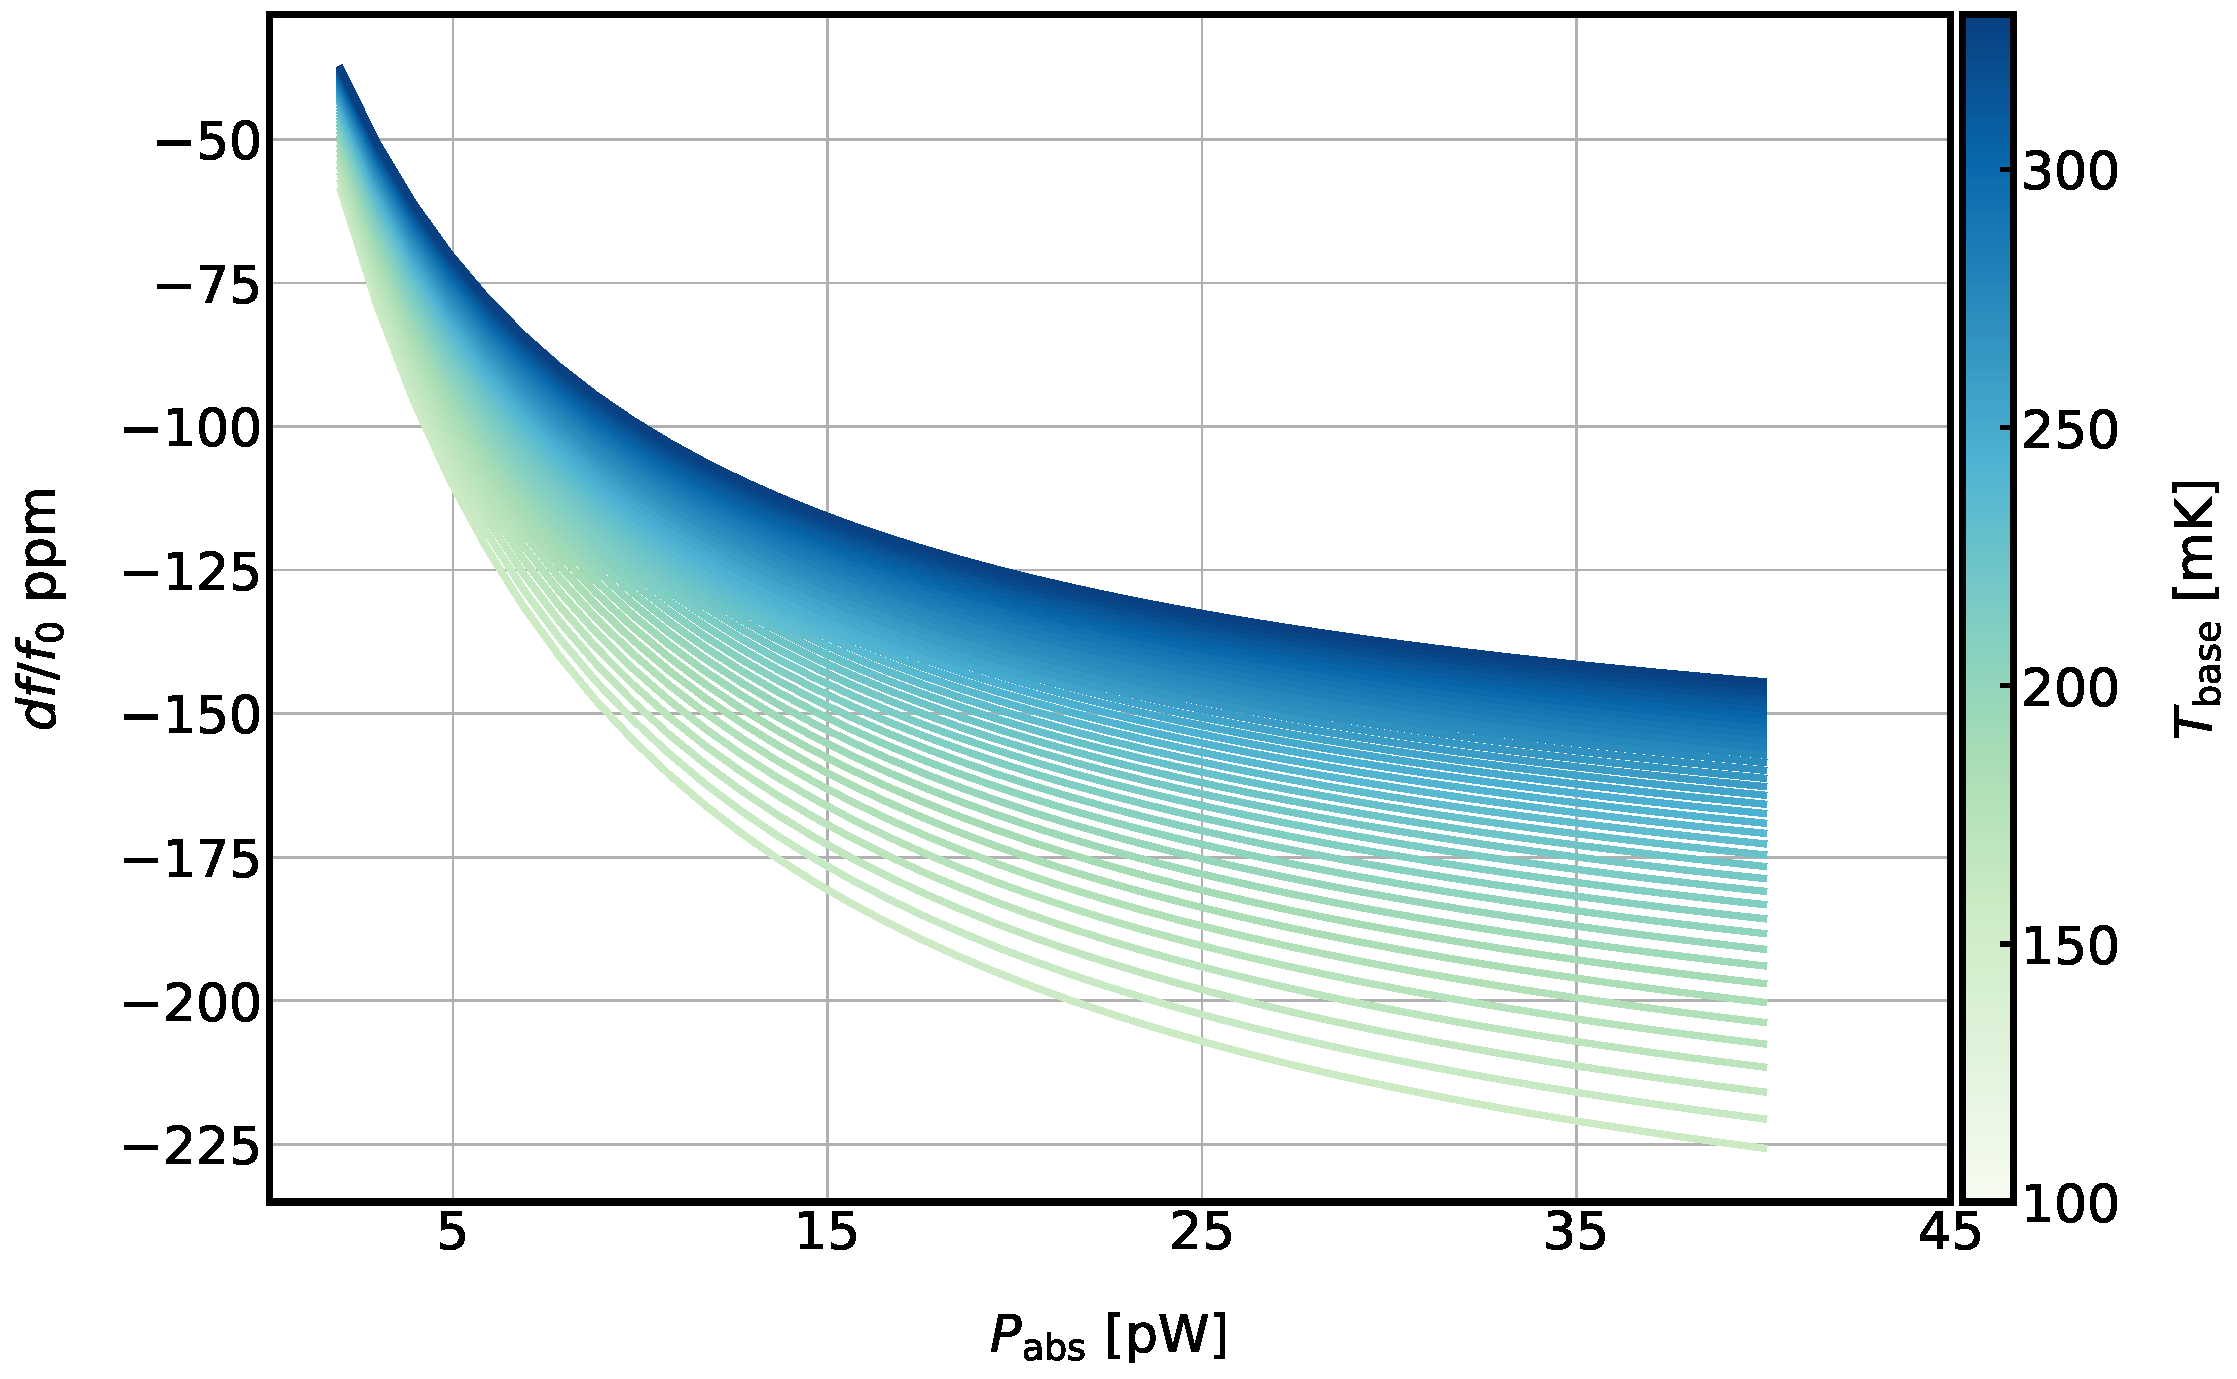
\includegraphics[width=0.8\textwidth]{figures/kid_model/resp_case2_T}
\caption[~The case~2 responsivity shown for a range of base temperatures.]{The \textit{Case 2} responsivity shown for a range of base temperatures.}
\label{fig:case 2 responsivity}
\end{figure}

A model of the \textit{Case 1} and \textit{Case 2} responsivities is shown in Figure~\ref{fig:responsivity}. In \textit{Case 1}, the frequency shift due to absorbed power, in fractional frequency units ($df_{0}/f_{0}$) is linear. In \textit{Case 2}, the frequency shift is approximately linear for low amounts of absorbed power, then asymptotically approaches a constant value at higher powers. Figure~\ref{fig:case 2 responsivity} shows the \textit{Case 2} responsivity for a range of base temperatures. The slope of the low-power, linear part of the curve becomes steeper at lower \gls{Tbase}.

\subsection{The Nonlinear Kinetic Inductance}\label{nonlinearKI}

The KI has a second-order term whose effects on various LEKID parameters must be considered during the biasing stage of detector calibration. The nonlinear KI can be written as a function of internal current, $I_{\mathrm{int}}$:

% Nonlinear KI
\begin{equation} \label{eq:nonlinear KI}
  \gls{Lk_per_l}(I_{\mathrm{int}}) = \gls{Lk_per_l}(0) \left[ 1 + \left( \frac{I_{\mathrm{int}}}{I_{\star}} \right) \right]
\end{equation}

where $I_{\star}$ is the critical current corresponding to the maximum charge-carrier velocity before pair-breaking occurs (\citet{tinkham2004introduction,anlage1989current,annunziata2010tunable}). In a LEKID camera, the source of this internal current is the microwave probe tone generated by the readout system. For LEKIDs, the readout tone power, $P_{ro}$, at the device typically ranges from $\sim$-60 to -120 dBm.
The nonlinearity adds an additional frequency detuning $\delta x$, of $\mathcal{O}(I^{2}/I_{\star}^{2})$:

\begin{equation}
  \delta x = \frac{\delta \omega}{\omega_{0}} = -\frac{1\delta L}{2L} = \frac{\alpha}{2}\left( \frac{I}{I_{\star}} \right)^{2} = -\frac{E_{r}}{E_{\star}}
\end{equation}

where $E_{r}$ is the internal resonator energy, and $E_{\star} = LI_{\star}^{2}/2\alpha = \gls{N0} \Delta^{2} \Sigma/2$ is the condensation energy of the inductor (\citet{mauskopf2018transition,tinkham2004introduction}). As in Section~\ref{sec:kinetic_inductance}, the resonator current is related to the internal resonator energy by the inductance (here assuming that $L_{m} \ll L_{K}$). The resonator energy can be written as a function of tone power \citep{swenson2013operation}, as:

% Resonator energy
\begin{equation}
 \begin{aligned}
  E_{r} &= \frac{1}{2}LI_{\mathrm{int}}^{2}\\
        &= \frac{2\gls{Qr}^{2}}{\gls{Qc}}\frac{1}{1 + 4\gls{Qr}^{2}x^{2}}\frac{P_{ro}}{\omega_{r}}
  \end{aligned}
\end{equation}

where $\omega_{r}$ is the shifted resonant frequency.

The total fractional detuning, $x$, is an implicit equation:

\begin{equation} \label{eq:implicit detuning}
  \begin{aligned}
  x &= x_{0} + \delta x \\
    &= x_{0} -\frac{E_{r}(x)}{E_{\star}}
    \end{aligned}
\end{equation}

Using the relations above, it's possible to estimate the degree of nonlinearity from a frequency sweep of  \gls{S21}. In standard practice, it's preferable to bias each resonator so that the frequency detuning contributed by the readout tone power is less than one resonator line-width (FWHM). This ensures that the resonator doesn't bifurcate. The width of the resonator is $\delta \omega \simeq \omega_{0}/\gls{Qr}$. Therefore, the fractional detuning due to the nonlinearity should be: $\left| \delta x \right| = \frac{E_{r}}{E_{\star}} < \frac{1}{\gls{Qr}}$. Using the equations above, satisfying this condition requires that an upper limit to the internal resonator energy is:

% maxmimum resonator energy before bifurcation
\begin{equation}
  E_{r} < \frac{\gls{N0}\gls{Delta}^{2}\Sigma}{2\gls{Qr}}
\end{equation}

and the maximum readout tone power is:

% maximum readout power before nonlinearity
\begin{equation} \label{eq:Pmax}
  P_{ro} < \frac{\gls{Qc}}{2\gls{Qr}^{3}}\gls{N0}\Delta^{3}\Sigma\omega\left(1 + 4\gls{Qr}^{2}x^{2} \right)
\end{equation}

At a fixed base temperature, larger optical loading permits the use of higher probe tone powers. This behavior is illustratd in Figure~\ref{fig:Pmax}, which shows the maximum probe tone power for a range of optical powers.

\begin{figure}[!htbp]
\centering
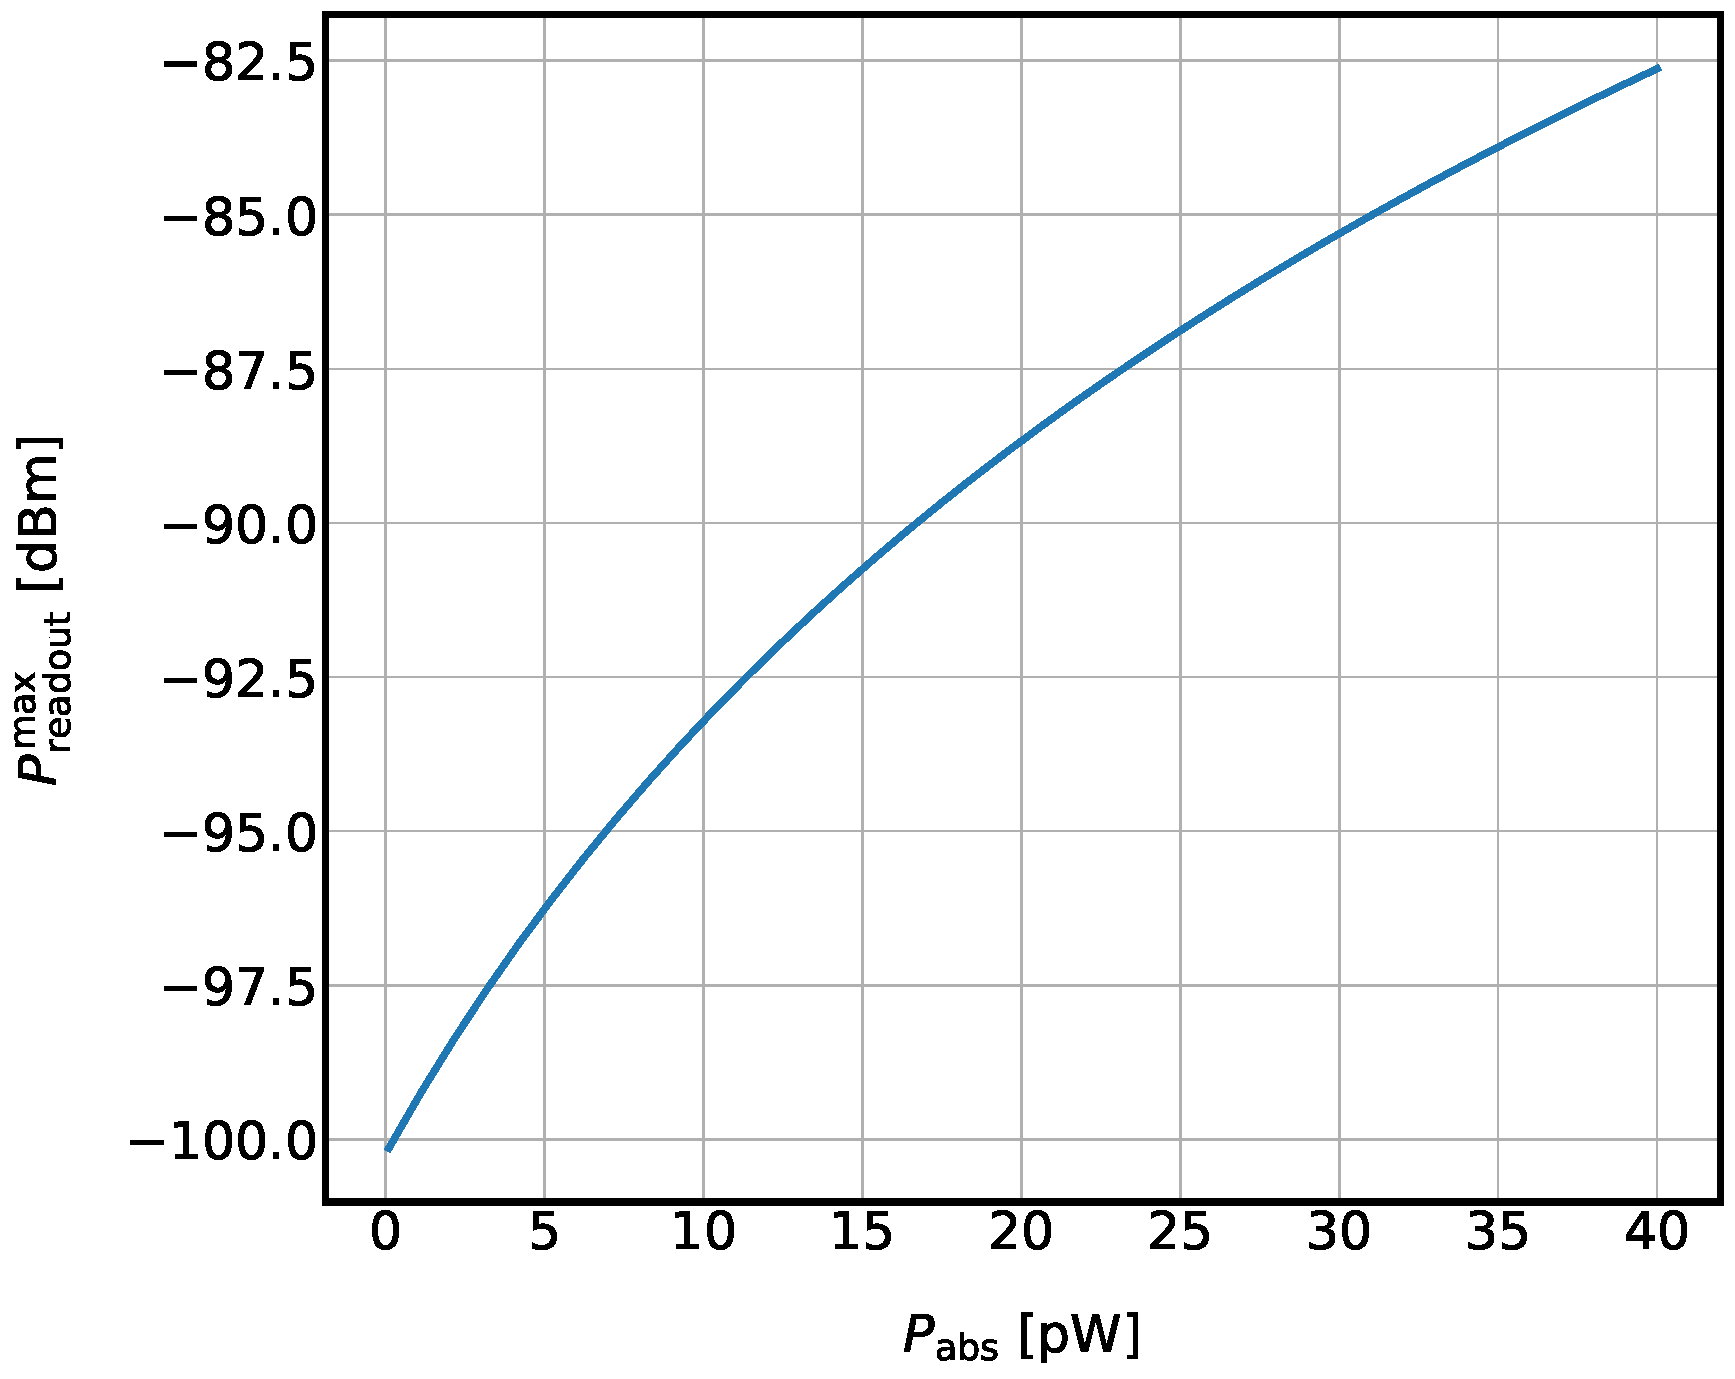
\includegraphics[width=0.8\textwidth]{figures/kid_model/Pmax}
\caption[~The maximum probe tone power shown for a range of optical power loadings.]{The maximum probe tone power shown for a range of optical power loadings.}
\label{fig:Pmax}
\end{figure}

\subsection{Bifurcation}\label{bifurc}

At a particular probe tone power, the resonance enters an unstable equilibrium between two states, which is known as bifurcation. This phenomenon can be understood from the persepective of soft-spring Duffing effects (see, e.g., \citet{swenson2013operation,duffing1918erzwungene}). Bifurcation can be induced during an \gls{S21} frequency sweep, by sweeping the resonance either from below or from above the resonant frequency. These two cases correspond to positive and negative feedback, respectively.

\textit{Upward sweep, positive feedback}:
As the probe tone is swept upward in frequency from below the resonant frequency, the resonant frequency is detuned, and drawn toward the probe tone frequency. This positive feedback increases until the resonator bifurcates between the energized state and its rest state.

\textit{Downward sweep, negative feedback}:
As the probe tone is swept downward in frequency from below the resonant frequency, the resonator is detuned farther below the probe tone frequency. When the probe tone eventually passes the resonant frequency, the resonator bifurcates between its energized and rest states.

The bifurcation power can be estimated using Equation~\ref{eq:Pmax}. If the resonator quality factor is dominated by the coupling quality factor, $\gls{Qr} \approx \gls{Qc}$, and $x \ll 1$,

% bifurcation power
\begin{equation} \label{eq:Pbifurc}
  P_{\mathrm{bifurc}} = \frac{1}{2 \gls{Qc}^{2}}\gls{N0}\Sigma \omega_{0}\Delta^{2}
\end{equation}

\section{Sensitivity} \label{sec:sensitivity}

The sensitivity of a sub-mm detector is typically reported as either a noise-equivalent power (NEP) or Noise-equivalent temperature (NET). The NEP (NET) describes the detector's sensitivity to absorbed optical power (temperature). NEP is commonly written in units of $\mathrm{W}/\sqrt{\mathrm{Hz}}$. This represents the noise power inside a measurement bandwidth of 1~Hz. Equivalently, it is the noise power which is measured after a 0.5~second integration (by the Shannon-Nyquist sampling theorem). At the time of writing, typical KID NEPs (under optical loading) are of $\mathcal{O}(10^{-17})$~$\mathrm{W}/\sqrt{\mathrm{Hz}}$. With that NEP, one can measure a signal level of $10^{-17}$~W with a signal-to-noise-ratio (SNR) of 1, over a 0.5~s integration.

KIDs, like most other astronomical detectors, are designed to be photon noise limited. Photon noise follows Poisson, or shot noise statistics. In a measurement dominated by shot noise, the SNR increases as $\sqrt{N}$, where $N$ is the number of measurements. In a typical sub-mm observation, the detector noise is limited by the shot noise of the background of in-band photons emanating from the receiver, optical system, atmosphere and astronomical source. In this scenario, the detectors are said to be operating in the background-limited IR photodetector (BLIP) limit.

During an on-sky KID measurement, it is preferable to view the detector timestreams in units of frequency shift (or fractional frequency) \gls{df}, relative to the resonant frequency of each pixel. If a responsivity (e.g., $df/dT$, $df/dP$) is known, then the NEP (or NET) can be calculated by dividing the square-root of the power spectral density (PSD) of the frequency fluctuations (units of Hz/$\sqrt{\mathrm{Hz}}$) by the corresponding responsitivity.

\subsection{Instrumental Noise Hierarchy}

The NEP which is calculated during a measurement is the sum of contributions from several different noise sources. The order in which each noise source should dominant constit the instrumental noise hierarchy. In a LEKID camera, the noise hierarchy (from most to least dominant) is:

\begin{itemize}[nosep]
  \item Photon noise
  \item Amplifier noise (dominated by the first-stage cryogenic low noise amplifier (LNA))
  \item Detector noise (generation-recombination (GR))
  \item Readout noise
\end{itemize}

The readout noise is discussed in \ref{readout}. The other three noise sources are treated individually in the following sections.

\subsection{Generation-Recombination Noise}\label{ssec:GR noise}

In the absence of readout and amplifier noise, the intrinsic noise floor of a KID measurement is set by GR noise. GR noise originates from the instantaneous uncertainty in the rate of CPs recombining into QP (or, equivalently, the rate at which CPs are broken into QP pairs). A simple expression for the GR contribution to the fractional noise spectral density follows from a consideration of the generation and recombination rates (\gls{gen_rate} and \gls{rec_rate}), assuming a steady state ($\gls{gen_rate} = \gls{rec_rate}$). The uncertainty in the number of CPs is:

\begin{equation}\label{eq:dNcp1}
  \begin{aligned}
  \delta N_{cp} &= \gls{gen_rate}\delta t - \gls{rec_rate}\delta t \\
                &= \sqrt{(\gls{gen_rate} + \gls{rec_rate})\delta t} \\
                &= \sqrt{2\gls{rec_rate}\delta t}
  \end{aligned}
\end{equation}

where $\delta t = 1/2 \delta f$ is the measurement integration time (with measurement bandwidth $\delta f$). Using the fact that $\gls{rec_rate} = \frac{\gls{Nqp}}{2\gls{tau_qp}}$, the uncertainty in the recombination rate is:

\begin{equation}
  \begin{aligned}
  \delta \gls{rec_rate} &= \frac{\delta N_{cp}}{\delta t} \\
                        &= \sqrt{ \frac{2\gls{rec_rate}}{\delta t}} \\
                        &= \sqrt{ \frac{2\gls{Nqp}}{2\gls{tau_qp}\delta t} }
  \end{aligned}
\end{equation}

Equation~\ref{eq:dNcp1} becomes:

\begin{equation}\label{eq:dNcp2}
  \begin{aligned}
  \delta N_{cp} &= \delta \gls{rec_rate} \gls{tau_qp} \\
                &= \sqrt{ \frac{\gls{Nqp} \gls{tau_qp}}{\delta t} } \\
                &= \sqrt{2\gls{Nqp}\gls{tau_qp} \delta f}
  \end{aligned}
\end{equation}

Dividing Equation~\ref{eq:dNcp2} by the square-root of the measurement bandwidth, and multiplying by the frequency responsivity to fluctuations in the number of QP yields an expression for the frequency noise PSD:

\begin{equation} \label{eq:ef GR}
e_{f,GR} = \sqrt{2 \gls{Nqp}_{\mathrm{,tot}}\gls{tau_qp}}\frac{df_{0}}{d\gls{Nqp}}
\qquad \left[ \frac{\mathrm{Hz}}{\sqrt{\mathrm{Hz}}} \right]
\end{equation}

From Equation~\ref{eq:ef GR}, the NEP contribution from GR can be calculated as:

\begin{equation} \label{eq:NEP GR}
  NEP_{GR} = e_{f,GR} \bigg/ \left( \frac{df_{0}}{d\gls{Nqp}}\frac{d\gls{Nqp}}{d\gls{Popt}} \right) \qquad \left[ \frac{\mathrm{W}}{\sqrt{\mathrm{Hz}}} \right]
\end{equation}

\subsection{Two-Level System Noise}\label{ssec:TLS}

Nonthermal two-level system (TLS) fluctuations occur throughout the amorphous dielectric layer of the superconducting substrate. The TLS systems have electric and magnetic dipoles which can interact with external fields around the device. These interactions manifest as fluctuations in the complex permittivity and/or permeability of the material. In a KID, random fluctuations in $C_{r}$ are indistinguishable from fluctuations in KI, because both introduce jitter to the resonant frequency. The TLS noise is generally modeled as being capacitive in origin (see, e.g., \citet{gao2008physics,zmuidzinas2012superconducting}). It is thought to be the underlying cause of an often observed anomalous increase in resonant frequency with increasing base temperature (a violation of predictions made by MB theory), however other explanations have been offered (see, e.g., the Kondo effect \citep{noguchi2018analysis}).

The TLS loss tangent, $\delta_{TLS}$, can limit the \gls{Qi} of a KID, and has an empirical dependence on the internal power stored in the resonator (proportional to microwave probe tone power), expressed as (\citet{barry2014development,martinis2005decoherence}):

\begin{equation}
  \delta_{TLS} = \gls{Qi}^{-1} = F_{TLS}\delta_{0} \left(\frac{1}{1 + \left| P_{\mathrm{int}}/P_{c} \right|} \right)^{1/2}
\end{equation}

where:
\begin{itemize}[label={},nosep]
  \item $F_{TLS}$ is the ratio of the electric field stored in the TLS systems to the total electric field
  \item $\delta_{0}$ is the intrinsic loss tangent
  \item $\chi = \hbar\omega/2kT$
  \item $P_{\mathrm{int}}$ is the internal resonator microwave power
  \item $P_{\mathrm{sat}}$ is the TLS saturation power
\end{itemize}

where the $\delta_{TLS}$ is known to saturate above a characteristic power, $P_{\mathrm{sat}}$. Because the maximum microwave readout power which can be used before nonlinearity sets in (Equation~\ref{eq:Pmax}) is proportional to inductor volume ($P_{ro\mathrm{,max}} \propto \Sigma$). The TLS noise therefore increases as $\Sigma^{1/2}$. The number of TLS systems scales with the volume of the amorphous dielectric, or $\Sigma$, and the way in which the KID responsivity varies with $\Sigma$ depends on the substrate material (see Section~\ref{sec:responsivity}).

For Al KIDs, the responsivity does not depend on $\Sigma$ (Equation~\ref{eq:case1}). The TLS noise therefore increases relative to GR and other noise sources as $\Sigma^{1/2}$, and the inductor volume can be made large. In TiN KIDs, $df_{0}/d\gls{Pabs} \propto \Sigma^{-1}$, and these devices typically use smaller $\Sigma$ \citep{mauskopf2018transition}. TLS noise mitigation techniques which involve the use of crystalline, rather than amorphous dielectrics, are presently an active area of research (see, e.g., \citet{weber2011single}).

A semi-empirical model for the TLS noise spectral density is presented in \citet{gao2008semiempirical}. The noise PSD has a colored spectrum ($\gls{Sxx} \propto f^{-\alpha}$) with spectral index $\alpha \approx 0.5$, and depends on microwave readout power and \gls{Tbase} as:

\begin{equation}\label{eq:Sx_TLS}
  \gls{Sxx}_{,TLS} \propto T^{-t}P_{ro}
\end{equation}

where $t = 1.5 -- 2$. $NEP_{TLS}$ can be found by dividing Equation~\ref{eq:Sx_TLS} by a responsivity (e.g., \gls{Rtemp} or \gls{Ropt}).

\subsection{Amplifier Noise}\label{ssec:amp noise}

The LNA which is used to amplify the probe tone comb at the output of the KID array adds thermal, or Johnson-Nyquist noise to the signal (\citet{johnson,nyquist1928thermal}). Johnson-Nyquist noise in a resistor originates from thermal motions of the electrons which manifest as voltage fluctuations across its terminals. Following \citet{kittel1998thermal}, an expression for the RMS voltage contribution from Johnson-Nyquist noise is found by considering a simple circuit model. The circuit consists of a white noise generator with resistance $R$ which transfers power to a resistive load with resistance $R_{L}$. The power transferred from the noise generator to the load is:

\begin{equation}
  P = \left<I^{2}\right>R_{L} = \frac{\left<V^{2}\right>R}{(R + R_{L})^{2}}
\end{equation}

The maximum power transfer occurs when the source and load are perfectly matched ($R = R_{L}$). In this case,

\begin{equation}
 P = \frac{\left<V^{2}\right>R}{4R}
\end{equation}

and the RMS voltage is:

\begin{equation}
  \left<V^{2}\right> = 4PR = 4kT\int_{f_{0}}^{f_{1}} R df = 4kTRB
\end{equation}

where $T$ is the temperature of the Thevenin equivalent of the circuit, and $B$ is the bandwidth over which the voltage is being measured. The resistance is assumed to be constant with frequency. Returning to the case of the LNA, the one-sided PSD of the voltage fluctuations is:

\begin{equation} \label{eq: johnson noise}
   e_{V,\mathrm{amp}} = 4kT_{\mathrm{amp}}Z \qquad  \left[ \frac{\mathrm{V}^{2}}{\mathrm{Hz}} \right]
\end{equation}

where $Z = R$ is the input impedance of the amplifier. The PSD is converted to frequency units by dividing by the voltage responsivity:

\begin{equation} \label{eq:ef amp}
  \begin{aligned}
  e_{f,\mathrm{amp}}^{2} &= \frac{e_{v,\mathrm{amp}}^{2}}{\left| dV/df_{0} \right|^{2}} \\
  \end{aligned}
\end{equation}

The voltage responsivity can be approximated using Equation~\ref{eq:S21}:

\begin{equation}
  \begin{aligned}
  \frac{dV_{\mathrm{out}}}{df_{0}} &= V_{\mathrm{in}}\frac{d\gls{S21}}{df_{\mathrm{out}}} \\
                         &\simeq -2jV_{\mathrm{in}}\frac{\gls{Qr}^{2}f_{\mathrm{probe}}}{\gls{Qc}f_{0}^{2}}\frac{1}{(1 + 2j\gls{Qr}x)^{2}}
  \end{aligned}
 \end{equation}

Near resonance, $x \ll 1$, and

\begin{equation}
  \frac{dV_{\mathrm{out}}}{df_{0}} \simeq 2jV_{\mathrm{in}}\frac{\gls{Qr}^{2}}{\gls{Qc}f_{0}}
\end{equation}

Equation~\ref{eq:ef amp} can then be written as:

\begin{equation}
  \begin{aligned}
  e_{f,\mathrm{amp}}^{2} &= 4kT_{\mathrm{amp}}Z_{0}\left( \frac{\gls{Qc}^{2}f_{0}^{2}}{4\gls{Qr}^{4}} \right) \\
               &= kT_{\mathrm{amp}}\left( \frac{\gls{Qc}^{2}f_{0}^{2}}{\gls{Qr}^{4}P_{ro}}\right) \\
               &= kT_{\mathrm{amp}}\left( \frac{f_{0}^{2}}{\gls{Qr}^{2}P_{ro}}\right)
  \end{aligned}
\end{equation}

where the probe tone power $P_{ro} = V_{\mathrm{in}}^{2}/Z_{0}$. For a resonator limited by the coupling quality factor ($\gls{Qr} \approx \gls{Qc}$),

\begin{equation}
  e_{f,\mathrm{amp}}^{2} = kT_{\mathrm{amp}}\left( \frac{f_{0}^{2}}{\gls{Qr}^{2}P_{ro}}\right) \qquad \left[ \frac{\mathrm{Hz}^{2}}{\mathrm{Hz}} \right]
\end{equation}

Therefore, for a probe tone near the resonant frequency, the frequency noise decreases with increasing readout power. As the tone power approaches the bifurcation power (Equation~\ref{eq:Pbifurc}), the frequency noise becomes independent of tone power. The LNA contribution to the NEP can therefore be written as:

\begin{equation}\label{eq:NEP amp}
  NEP_{\mathrm{amp}} = e_{f,\mathrm{amp}} \bigg/ \left( \frac{df_{0}}{d\gls{Nqp}}\frac{d\gls{Nqp}}{d\gls{Popt}} \right) \qquad \left[ \frac{\mathrm{W}}{\sqrt{\mathrm{Hz}}} \right]
\end{equation}

The $NEP_{\mathrm{amp}} \propto 1/\sqrt{P_{ro}} $ dependence makes it possible to suppress the amplifer noise contribution by using higher microwave readout powers.

\subsection{Photon Noise} \label{photon noise}

The optical power input into the system is assumed to be incoherent emission from a thermal blackbody source. To write an expression for the total optical power \gls{Popt}, we first consider the number of modes contained in the incident light beam, which has a central frequency $\nu$ and optical bandwidth $\Delta \nu$. The total number of modes is the product of the number of spatial, temporal and polarization modes:

\begin{equation}
 \begin{aligned}
  N_{\mathrm{modes}} &= \left( N_{\mathrm{spatial}} \right) \left( N_{\mathrm{temporal}} \right) \left( N_{\mathrm{pol}} \right) \\
            &= \left( \frac{A\Omega\nu^{2}}{c^{2}} \right) \left(\tau_{\mathrm{int}}\Delta \nu \right) \left(m\right)
  \end{aligned}
\end{equation}

where:
\begin{itemize}[label={},nosep]
  \item $A\Omega$ is the $\acute{e}$ntendue
  \item $\nu^{2}/c^{2} = \lambda^{2}$ is the $\acute{e}$ntendue of coherence
  \item $\tau_{\mathrm{int}}$ is the integration time
  \item $m$ is the number of polarization modes [1,2]
\end{itemize}

The photon arrival times follow Bose-Einstein statistics, with an occupation number, or mean number of photons per mode, of:

\begin{equation}
  \gls{n_occ} = \frac{\left< N_{\mathrm{photons}} \right> }{\mathrm{mode}} = \frac{1}{e^{h\nu/kT} - 1}
\end{equation}

where $T$ is the blackbody temperature of the source. With $m = 2$, the total optical power can be expressed as:

\begin{equation}\label{eq:P_opt}
 \begin{aligned}
  \gls{Popt} &= \left( N_{\mathrm{modes}} \times \frac{\left< N_{\mathrm{phot}} \right>}{\mathrm{mode}} \times \textrm{Energy per photon} \right) \bigg/ \tau_{\mathrm{int}} \\
          &= \left( \frac{m A\Omega\nu^{2}}{c^{2}} \right) \left(\tau_{\mathrm{int}}\Delta \nu \right)  \gls{n_occ} \frac{h\nu}{\tau_{\mathrm{int}}} \\
          &= A\Omega\Delta\nu \left( \frac{2h\nu^{3}}{c^{2}}\frac{1}{e^{h\nu/kT} - 1} \right) \\
          &= A\Omega\Delta\nu B_{\nu}(\nu, T) \qquad \left[ \mathrm{W} \right]
  \end{aligned}
\end{equation}

where $B_{\nu}(\nu, T)$ $\left[ \mathrm{W}\mathrm{m}^{-2}\mathrm{ str }^{-1}\mathrm{Hz}^{-1} \right]$ is the Planck function for spectral radiance. The incident power which is absorbed by the detectors is the total optical power multiplied by the optical efficiency \gls{opt_eff} and quantum efficiency of the detectors \gls{det_eff}:

\begin{equation}\label{eq:P_abs}
  \begin{aligned}
  \gls{Pabs} &= \gls{opt_eff}\gls{det_eff}\gls{Popt} \\
          &= \gls{opt_eff}\gls{det_eff} A\Omega\Delta\nu B_{\nu}(\nu, T) \qquad \left[ \mathrm{W} \right]
  \end{aligned}
\end{equation}

The mean-squared noise power measured by the detectors originates from fluctuations in \gls{n_occ}. Because its probability distribution function is the Bose-Einstein distribution, its variance is:

\begin{equation}
  \sigma^{2}_{n_{occ}} = \gls{n_occ} + \frac{ \gls{n_occ}^{2} }{N_{\mathrm{modes}}}
\end{equation}

where a factor corresponding to the case of $N_{\mathrm{modes}} \ll 1$ has been omitted (see, e.g., \citet{fox2006quantum,rowe2015passive}). The mean-squared noise power input to the optical system is therefore

\begin{equation}\label{eq:sigma_P}
  \begin{aligned}
  \sigma^{2}_{P} &= \sigma^{2}_{n_{occ}}N_{\mathrm{modes}}\left( \frac{h\nu}{\tau_{\mathrm{int}}} \right)^{2} \\
                 &= \frac{h\nu \gls{Popt}}{\tau_{\mathrm{int}}} + \frac{\gls{Popt}^{2}}{N_{\mathrm{modes}}} \qquad \left[ \mathrm{W}^{2} \right]
  \end{aligned}
\end{equation}

The noise spectral density (square-root of the NEP) is found by dividing Equation~\ref{eq:sigma_P} by the measurement bandwidth, $B = f_{s}/2 = \tau_{\mathrm{int}}$:

\begin{equation}\label{eq:Sxx_Popt}
  S_{xx} =  NEP_{\mathrm{phot}}^{2} = h\nu \gls{Popt} + \frac{\gls{Popt}^{2}}{N_{\mathrm{modes}}B} \qquad \left[ \frac{\mathrm{W}^{2}}{\mathrm{Hz}} \right]
\end{equation}

When the NEP is expressed in terms of \gls{Popt}, it is referred to as the \textit{electrical} NEP. When the NEP is expressed in terms of \gls{Pabs}, it is referred to as the \textit{optical} NEP. The first term in Equation~\ref{eq:Sxx_Popt} dominates for low \gls{n_occ} (shot noise limit, $h\nu / kT \gg 1$), and the second term dominates for high occuption number (wave noise limit, $h\nu / kT \ll 1$):

\begin{equation}\label{eq:NEP phot}
NEP_{\mathrm{phot}}^{2} = NEP_{\mathrm{shot}}^{2} + NEP_{\mathrm{wave}}^{2} \\
\end{equation}

In each of BLAST-TNG's three observation bands (250, 350 and 500~$\upmu$m) the shot noise term dominates the NEP. In frequency units, the NEP can be calculated as:

\begin{equation} \label{eq:ef phot}
  e_{f,\mathrm{phot}} = NEP_{\mathrm{phot}}\frac{df_{0}}{dN_{qp}}\frac{dN_{qp}}{d\gls{Popt}} \qquad \left[ \frac{\mathrm{Hz}}{\sqrt{\mathrm{Hz}}} \right]
\end{equation}

\subsection{Total NEP}

In frequency units, the total noise spectral density measured by the detectors is the quadrature sum of the noise contributions from each of the sources discussed in the above sections:

\begin{equation} \label{eq:ef tot}
  e_{f} = \left( e_{f,\mathrm{phot}}^{2}  + e_{f,\mathrm{amp}}^{2} + e_{f,TLS}^{2} \right)^{1/2} \qquad \left[ \frac{\mathrm{Hz}}{\sqrt{\mathrm{Hz}}} \right]
\end{equation}

Figure~\ref{fig:Sxx_fracfreq} shows Equation~\ref{eq:ef tot} as a function of absorbed optical power (omitting the contribution from TLS). Photon noise is dominant for absorbed power between $\sim$1--18~pW, above which amplifier noise dominates due to the decrease in resonator quality factor $\gls{Qr}$. The physical parameters in this example simulation (which are representative of the BLAST-TNG 250~$\upmu$m array) predict white noise levels, in fractional frequency units, of a few $\times 10^{-17}$ [Hz$^{-1}$]. The ratio of the photon noise to the amplifier and GR noise is illustrated in Figure~\ref{fig:noise_ratios}. The photon noise dominates over the GR noise at absorbed powers of a few picowatts.

\begin{figure}[!htbp]
\centering
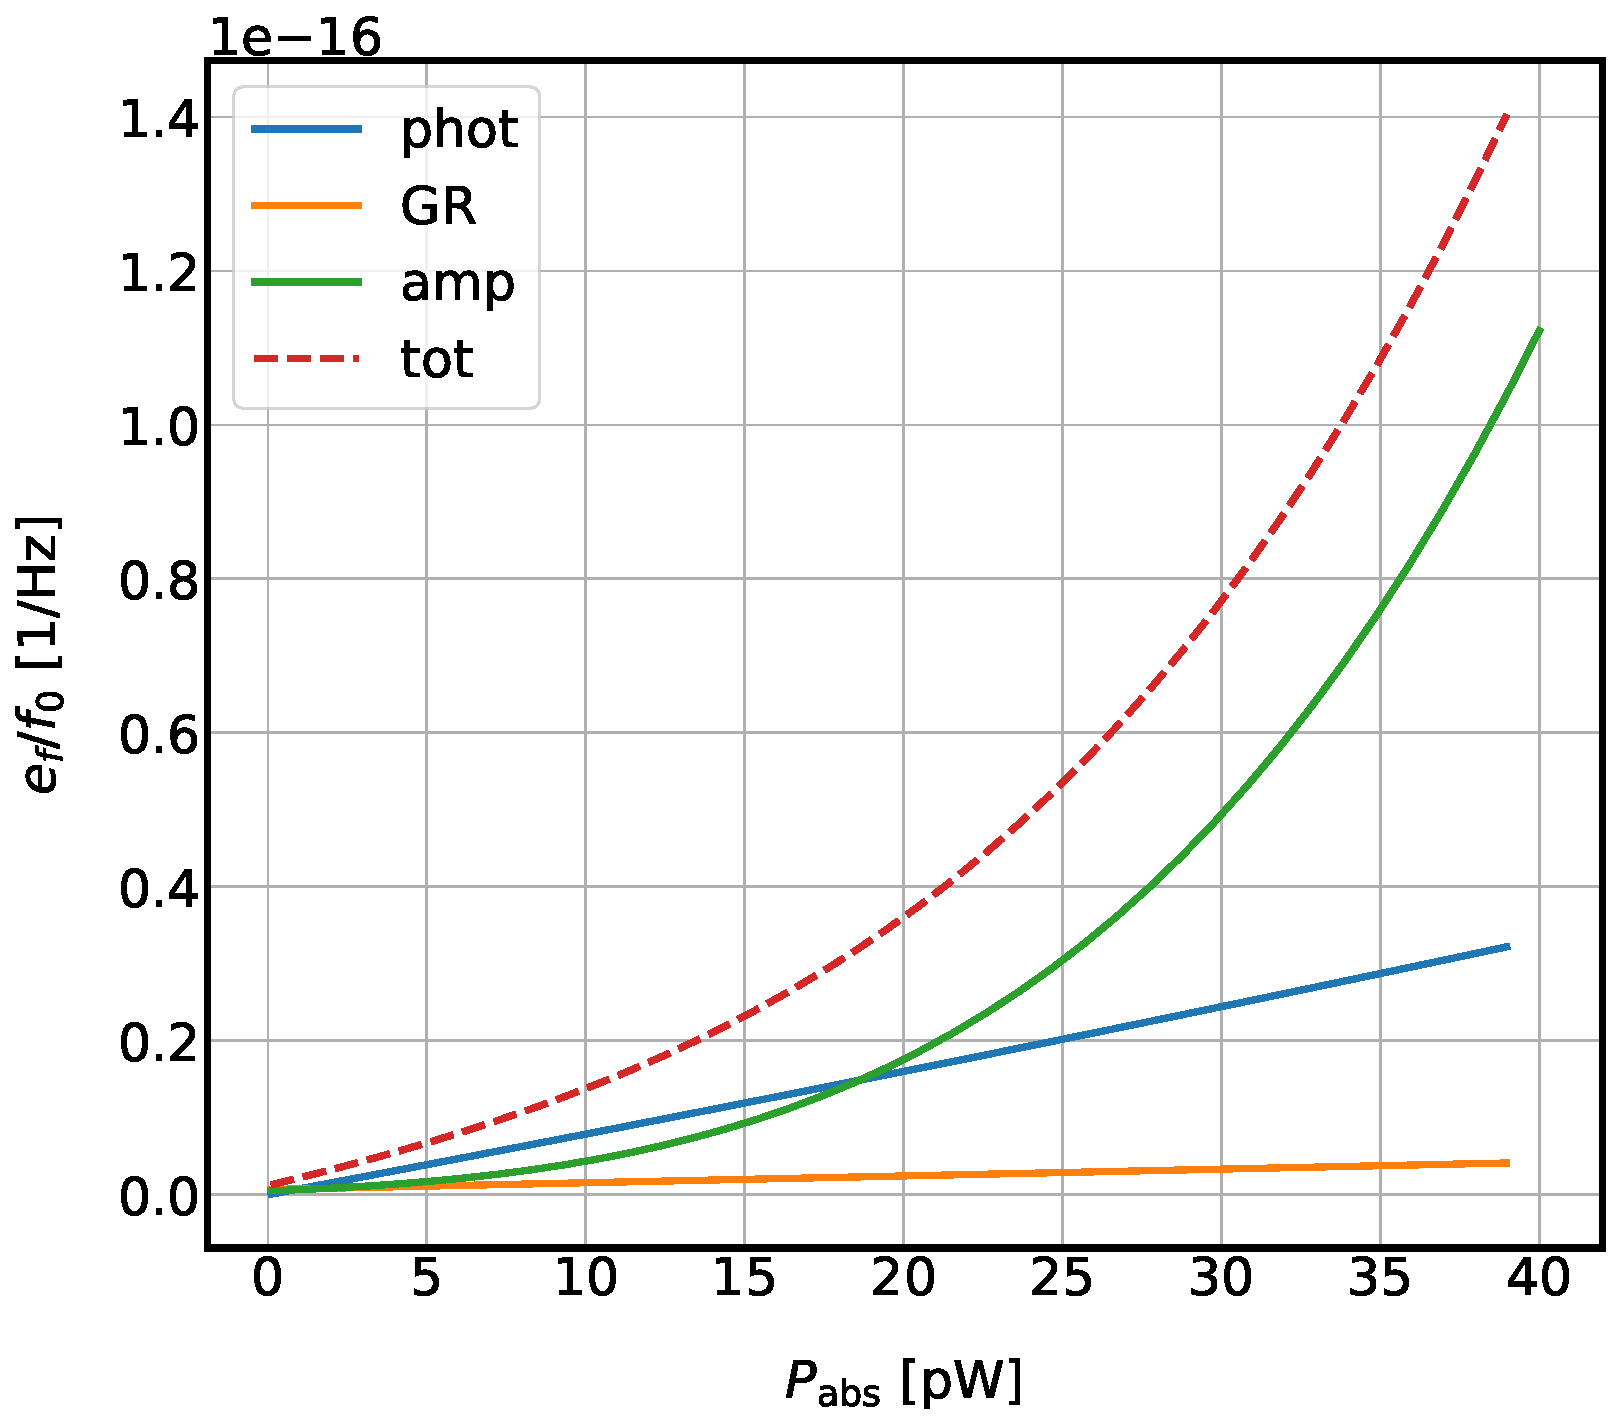
\includegraphics[width=0.8\textwidth]{figures/kid_model/Sxx_fracfreq}
\caption[~The spectral density, in fractional frequency units, as a function of optical power, for the major contributers of instrumental noise.]{The spectral density, in fractional frequency units, as a function of optical power, for the major contributers of instrumental noise.}
\label{fig:Sxx_fracfreq}
\end{figure}

\begin{figure}[!htbp]
\centering
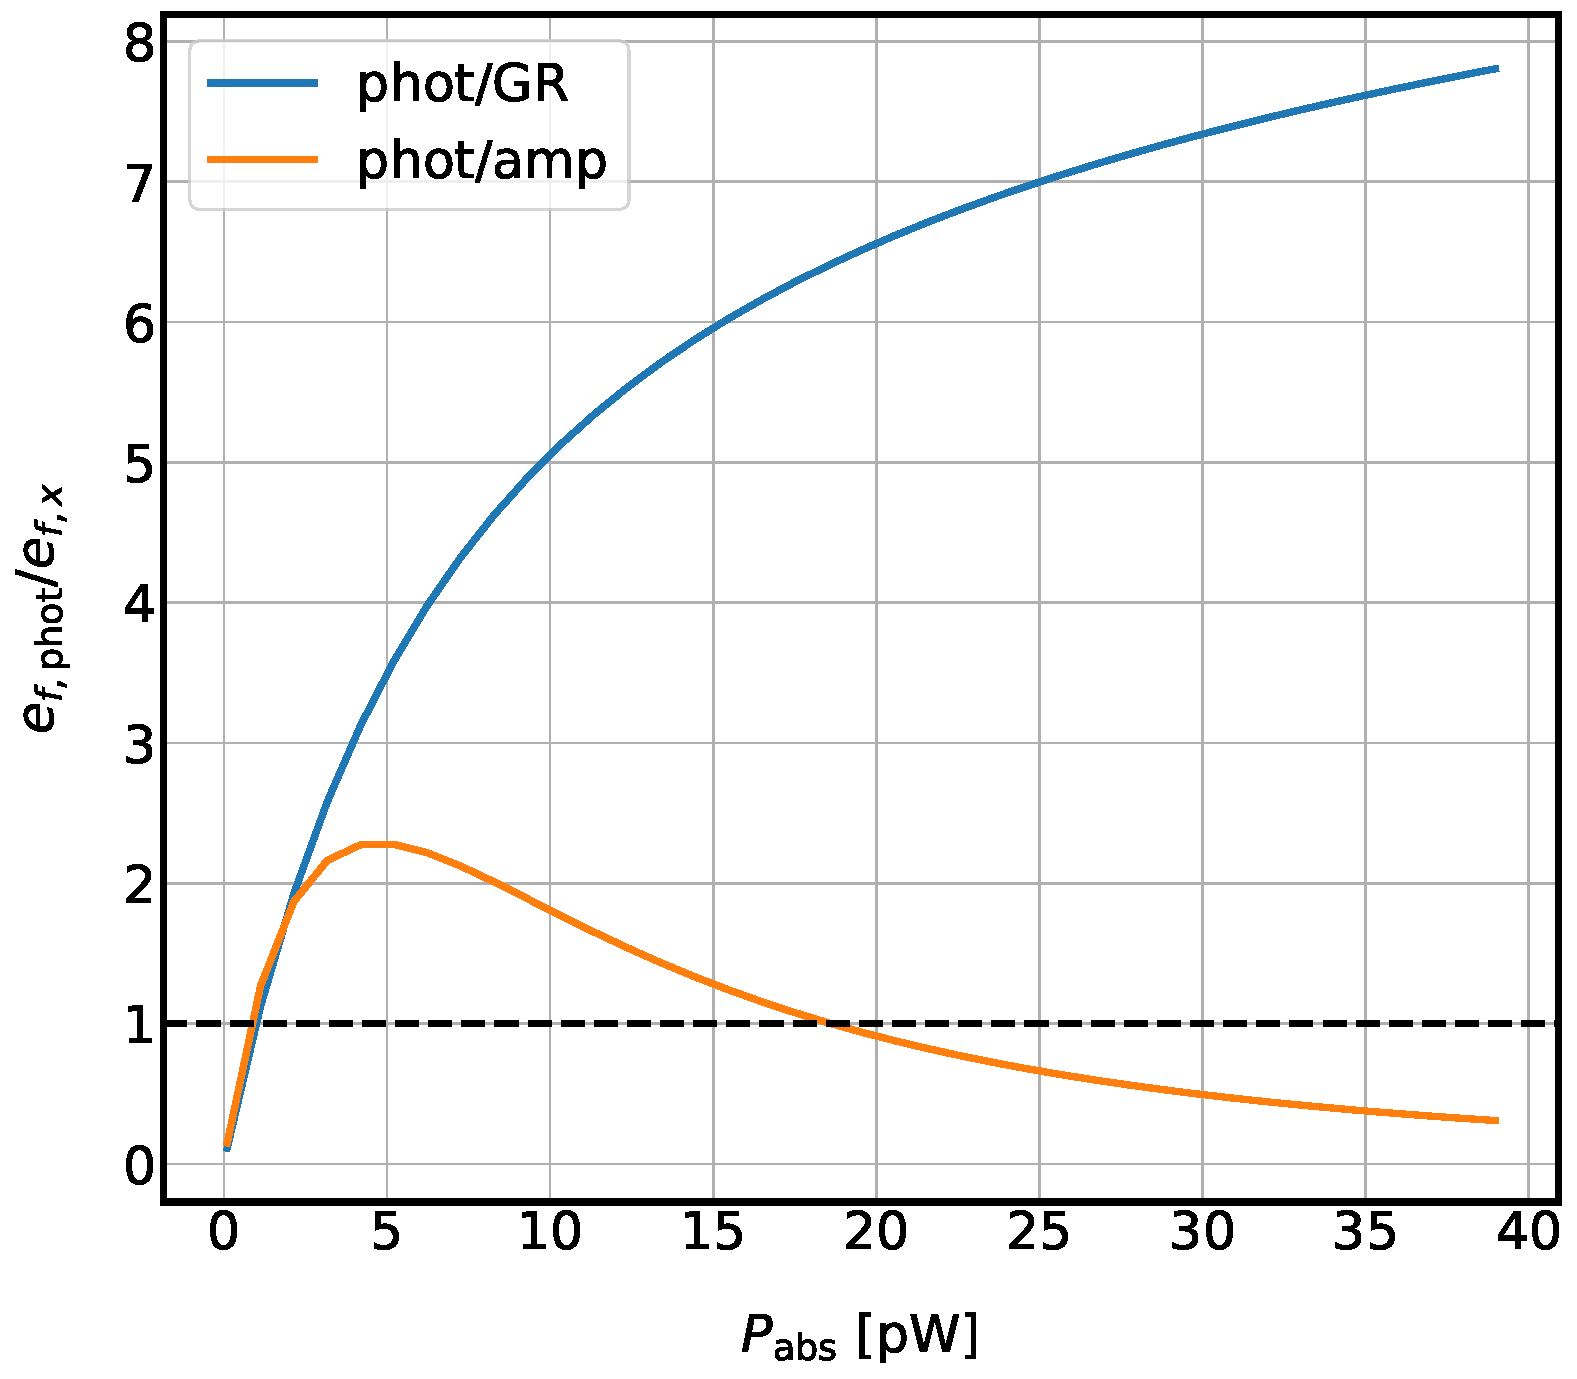
\includegraphics[width=0.8\textwidth]{figures/kid_model/noise_ratios}
\caption[~The simulated ratios of photon to GR and photon to amplifier noise.]{The ratio of $e_{f,phot}$ to $e_{f,GR}$ and $e_{f,\mathrm{amp}}$.}
\label{fig:noise_ratios}
\end{figure}

The total optical NEP is:

\begin{equation} \label{eq:NEP tot}
  NEP_{\mathrm{tot}} = \left( NEP_{\mathrm{amp}}^{2} + NEP_{GR}^{2} + NEP_{TLS}^{2} + NEP_{\mathrm{phot}}^{2} \right)^{1/2} \qquad \left[ \frac{\mathrm{W}}{\sqrt{\mathrm{Hz}}} \right]
\end{equation}

The NEP for each noise source (except for TLS) is shown in Figure~\ref{fig:NEP_tot}. At absorbed powers above a few picowatts, the simulated NEP is $\propto \sqrt{\gls{Popt}}$.

\begin{figure}[!htbp]
\centering
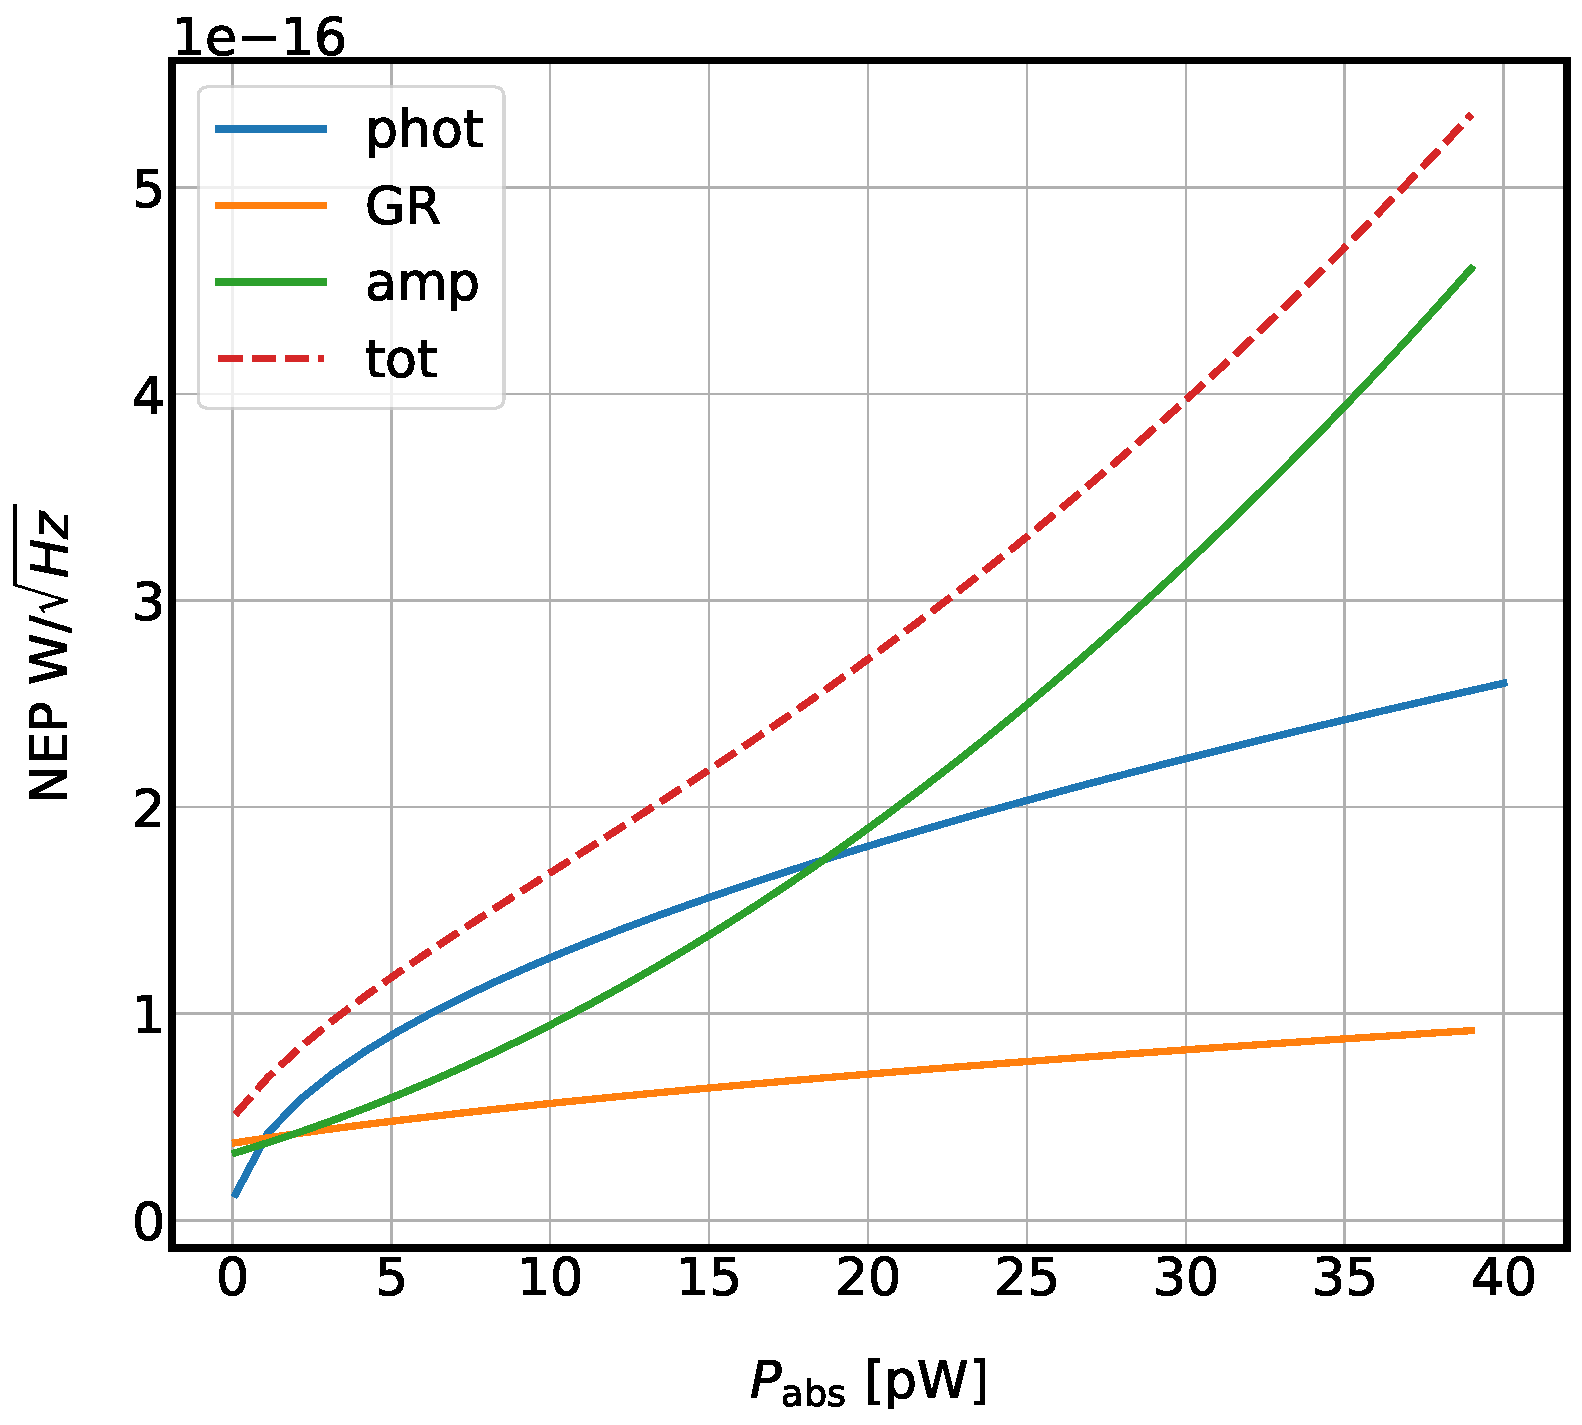
\includegraphics[width=0.8\textwidth]{figures/kid_model/NEP}
\caption[~The optical NEP as a function of optical power, for the major contributers of instrumental noise.]{The optical NEP as a function of optical power, for the major contributers of instrumental noise.}
\label{fig:NEP_tot}
\end{figure}

and the total NET can be calculated as:

\begin{equation} \label{eq:NET tot}
  NET_{\mathrm{tot}} = \frac{NEP_{\mathrm{tot}}}{k\gls{opt_eff}\Delta\nu} \qquad \left[ \frac{\mathrm{K}}{\sqrt{\mathrm{Hz}}} \right]
\end{equation}


\begin{comment}
\begin{equation}
  I = \Re(\gls{S21}) = 1 - \frac{\gls{Qr}}{\gls{Qc}}\frac{1}{1 + 4\gls{Qr}^{2}x^{2}}
\end{equation}

\begin{equation}
  Q = \Im(\gls{S21}) = \frac{\gls{Qr}}{\gls{Qc}} \frac{2\gls{Qr}x}{1 + 4\gls{Qr}^{2}x^{2}}
\end{equation}

\section{Detector Biasing} \label{biasing}
% nonlinearity parameter
\begin{equation}
  \alpha = \frac{2\gls{Qr}^{2}}{\gls{Qc}}\frac{P_{r}}{\omega_{\mathrm{shift}}E_{\star}(x)}
\end{equation}

% y, generator detuning (number of linewidths relative to power shifted, or low-power resonance)
\begin{equation}
  y = \gls{Qr}x = \left(\omega_{probe} - \omega_{shift}\right)/\Delta\omega
\end{equation}
where $\Delta \omega$ is the full-width-half-max (FWHM) width of the resonance.
\end{comment}
                     %   \include rather than \input for chapters
\chapter{Design of an FPGA-based LEKID spectrometer}\label{readout}

The ASU open-source LEKID readout is a 1000-channel transceiver, consisting of digital and analog electronics, firmware and software. This technology builds on the legacy of previous MKID demonstrator instruments which have used Field Programmable Gate Array (FGPA) platforms (e.g. MUSIC \citep{golwala2012status}, ARCONS \citep{mchugh2012readout}, NIKA \citep{monfardini2014latest}, MUSTANG-2 \citep{dicker2014mustang2}, MAKO \citep{swenson2012mako}, SPACEKIDS \citep{van2016multiplexed}, DARKNESS \citep{strader2016digitial}). FPGAs enable the high speed digital signal processing (DSP) techniques which are required for both time and frequency-domain-multiplexed readout (FDM) of superconducting detectors.

The FPGA board which serves as the foundation for the LEKID readout described in this work is the second generation Reconfigurable Open Architecture Computing Hardware (ROACH2), an open-source DSP board developed by the Collaboration for Astronomical Signal Processing and Electronics Research (\citet{werthimer2011casper, hickish2016decade}). The ROACH2 is a general purpose DSP board whose primary use is as a digital backend for radio astronomy observatories. The ASU LEKID readout, which is the subject of this chapter, is one of several MKID readouts which have used the ROACH1/ROACH2 platform, including MUSIC (ROACH1), MAKO (ROACH2), ARCONS (ROACH1/2) and DARKNESS (ROACH2/DARKNESS board).

The design and creation of the readout system was driven by a philosophy based on adaptability and scalability. Consequently, the system now serves as a core part of several current and upcoming astronomical instruments. Among these are balloon-borne (e.g., OLIMPO \citep{masi2019kinetic}, BLAST-TNG \citep{gordon2016}) and ground-based cameras (e.g, TolTEC \citep{austermann2018millimeter}, SuperSpec \citep{wheeler2018superspec}, MUSCAT \citep{brien2018muscat}).

In the following sections, we describe the design and verification of the LEKID readout system, with a primary focus on the system which has been developed for the BLAST-TNG stratospheric balloon platform. The chapter is organized as follows:

\begin{itemize}[nosep]
  \item Section~\ref{sys overview} provides a brief overview of the principal readout functions.
  \item Section~\ref{sys reqs} describes the primary system requirements.
  \item Section~\ref{firmware} details the design and verification of the ROACH2 firmware and DSP algorithms.
  \item Section~\ref{hardware and elec} describes the design and construction of the BLAST-TNG readout hardware and electronics.
  \item Section~\ref{noise verify} presents the results of noise verification measurements.
\end{itemize}

\section{System Requirements}\label{sys reqs}

The core system requirements for a KID readout system fall under cateogories of multiplexing factor, data rate, noise performance, size, weight, power and cost (SWAP-C) and timing synchronization. The readout system be able to read out the required number of LEKID detectors at a rate determined by the telescope scan speed while contributing less noise than the detectors and croygenic low-noise amplifiers (LNAs). To facilitate map mapping, the detector data packets must be timestamped in such a way that makes it possible to later align them with the timing information provided by the pointing system.

It is important to note that the requirements which are discussed here pertain primarily to sub-mm KID cameras. Optical/NIR (O/NIR) systems have slightly different requirements. The following sections discuss the motivation behind each requirement, which are listed in Table~\ref{tab:sys reqs}.

\begin{table}[!htbp]
\centering
\begin{tabular}{@{}ll@{}}
\dtoprule
Parameter & Requirement \\ \midrule
RF bandwidth (MHz) & 512 \\
\gls{Sphase} / chan (dBc/Hz) & $\lesssim$ -95 \\
1/f \gls{fc} (Hz) & $\lesssim$ 0.5 \\
Data rate (Hz) & 200--500 \\
Power dissipation (W) & $\lesssim$ 60 \\
Time stamp precision (ms) & $\lesssim$ 1 \\
DAC Tone Resolution (Hz) & $\leq$ 1000 \\
Multiplexing Factor & $\gtrsim$ 500 \\ \dbottomrule
\\
\end{tabular}
\caption{LEKID readout system requirements.}
\label{tab:sys reqs}
\end{table}

We begin with an overview of the system.

\subsection{System Overview}\label{sys overview}

The LEKID readout processes 512~MHz of instantaneous complex baseband and RF (radio frequency) bandwidth using quadrature ($I/Q$) signal processing. The total bandwidth is divided between 1000 channels, each with readout bandwidth of $\sim$30--500~Hz. For each channel, the system outputs a 64-bit $I/Q$ sample at a configurable data rate of $\sim$60--1000~Hz. The $I/Q$ pairs represent the total transmission of each resonator ($I + jQ = V_{\mathrm{in}}\gls{S21}$), and contain the AM (amplitude modulation) and PM (phase modulation) of the detectors. If the detectors are properly biased, the PM and FM is proportional to the absorbed optical power. For KID readout, typically only the PM is used.

In order to accurately probe the resonant frequency of each detector, the probe (carrier) tones synthesized by the DAC must have a frequency resolution $f_{\mathrm{res}} \lesssim 1000$~Hz (this requirement scales with the resonator quality factor \gls{Qr}).


To readout the detectors, the system must do the following:

\begin{enumerate}[nosep]
  \item Synthesize a baseband probe tone ($I_{DAC} + jQ_{DAC}$) in software and firmware with a unique amplitude, frequency and phase for each resonator.
  \item Generate the tone comb with the digital-to-analog converters (DACs).
  \item Upconvert the tone comb to the RF band of the detectors and send to the detector arrays.
  \item Receive the detector modulated tone comb.
  \item Downconvert the modulated tone comb from RF to baseband, amplify/attenuate/filter as needed.
  \item Digitize the tone comb and analyze with a polyphase filterbank/Fourier transform (PFB-FFT, see Section~\ref{pfb}).
  \item Discard unwanted FFT bins (remaining bins are labeled as channels).
  \item Digitally demodulate each channel (digital downconverter, see Section~\ref{ddc}).
  \item Optionally apply an FIR (finite impulse response) filter to the demodulated signals.
  \item Coherently accumulate each demodulated signal to filter and downsample to the desired output rate (see Section~\ref{accum}).
  \item Packetize $I$ and $Q$ for each channel into UDP frames, add timing and checksum information.
  \item Stream packets to the data network.
  \item In software, perform all necessary steps to calculate the FM of each resonator, and convert to absorbed optical power.
\end{enumerate}

\vspace{5mm}

\subsection{White Noise}\label{white noise}

The readout noise is characterized by its power spectral density (PSD), $S_{xx}$ $\left[\mathrm{x}^{2}/\mathrm{Hz}\right]$, which consists of additive white Gaussian noise (AWGN, hereafter WN) and 1/f (`one over f') components. The latter is hereafter referred to as flicker noise (FN). The 1/f knee, or corner-frequency \gls{fc} of the FN sets the lower limit on the telescope scan speed $\omega_{\mathrm{scan}}$ and readout rate $f_{ro}$ which will permit for adequate mapping of the science targets.

\begin{table}[!htbp]
\centering
\begin{tabular}{@{}lccc@{}}
\dtoprule
Array                      & 250~$\upmu$m & 350~$\upmu$m & 500~$\upmu$m   \\ \midrule
Readout Modules            & 3               & 1               & 1  \\ \midrule
Number of Tones per Module & $\sim$500             & $\sim$700             &  $\sim$300   \\ \dbottomrule
\\
\end{tabular}
\caption[~Detector counts for the three BLAST-TNG wavebands.]{Detector counts for the three BLAST-TNG wavebands. A detailed description of the detector counts is provided in Chapter 4 of this document.}
\label{tab:det counts}
\end{table}

The readout must meet its noise requirements at the highest multiplexing factor set by the pixel count of each detector array. BLAST-TNG's $\sim$2,500 detectors are divided between five independent readout slices: One each for the 350 and 500~$\upmu$m arrays, and three for the 250~$\upmu$m array. Each slice contains a ROACH2 board, DAC/ADC board and a set of both commercial-off-the-shelf (COTS) and custom-made RF electronics (see Section~\ref{hardware and elec}). Although the 250~$\upmu$m array could have been distributed between two readout slices, the array was designed as one chip which contains a set of three identical rhombuses. The $\sim$700 pixels of the 350~$\upmu$m array sets the most stringent multiplexing requirement on a single slice. Approximate detector counts for each BLAST-TNG band are listed in Table~\ref{tab:det counts}.

The requirement on the WN level of each readout channel is that it must be lower than that of both the LNA and detectors, at all multiplexing factors (see Chapter~\ref{kid_model} for a detailed description of the instrumental noise hierarchy). The FM of the resonators is in the phase quadrature of the signal, while the amplifier noise is in the dissipation quadrature. The phase of $I/Q$ is:

\begin{equation}
  \gls{phiIQ} = \arctantwo(Q,I)
\end{equation}

and its PSD \gls{Sxx} has units of $\mathrm{rad}^{2}/\mathrm{Hz}$. It is useful to express \gls{Sphase} in units of dBc/Hz (decibels relative-to-the-carrier, $10\log_{10}(\gls{Sphase})$). The amplifier and detector noise are commonly expressed using the PSD of their fractional frequency fluctuations \gls{Sff} [1/Hz] (see Chapter~\ref{kid_model}). Following \citet{gao2008physics}, \gls{Sphi} can be converted to \gls{Sff} using a known or estimated resonator quality factor, \gls{Qr}:

\begin{equation}\label{eq:Sff est}
  \gls{Sff} = \frac{S_{\phi}}{16 \gls{Qr}^{2}} \qquad \left[ \mathrm{Hz}^{-1} \right]
\end{equation}

by: $\frac{\delta f}{f} = \frac{\delta \phi}{4 \gls{Qr}}$. For LEKID detectors like the ones used in BLAST-TNG, the optically loaded detector noise is $\gls{Sff} \sim 10^{-17}$ $\mathrm{Hz}^{-1}$.

The frequency noise of the LNA \gls{Sff}$_{,\mathrm{amp}}$ can be estimated as \citep{barry2014development}:

\begin{equation}\label{eq:amp freq noise}
  \gls{Sff}_{,\mathrm{amp}} \simeq \frac{kT_{N}}{P_{pr}}\frac{\gls{Qc}^{2}}{\gls{Qr}^{4}}
\end{equation}

where $k$ is Boltzmann's constant, $T_{N}$ is the noise temperature of the LNA and $P_{ro}$ is the power in the microwave probe tone. For BLAST-TNG, $T_{N} \approx 6$~K. $P_{ro}$ ranges from -80 to -90~dBm at the detectors, and \gls{Qr} and \gls{Qc} range from $\sim$1--5 $\times$ 10$^{4}$. Using these ranges in Equation~\ref{eq:amp freq noise} suggests that a lower limit on \gls{Sff}$_{,\mathrm{amp}}$ is $\sim$5 $\times$ 10$^{-20}$ $\mathrm{Hz}^{-1}$. Converting this value to a phase noise using Equation~\ref{eq:Sff est} gives a required phase noise of $\lesssim$~-95~dBc/Hz.

The WN floor for a single probe tone is set by the bit-width of the analog-to-digital converters (ADCs). Given an effective number of bits (ENOB) and ADC sampling frequency $f_{s}$, this floor is:

\begin{equation}
-20\log_{10}(2^{ENOB})- 10\log_{10}(f_{s}/2) \qquad \left[ \frac{\mathrm{dBc}}{\mathrm{Hz}} \right]
\end{equation}

For an ENOB of 10-bits and $f_{s} = 512$~MHz (see Section~\ref{hardware and elec}), this noise floor is $\approx$-144~dBc/Hz. For a multitone comb of $N$ tones, the WN level of each tone can be estimated as:

\begin{equation}\label{eq:whitenoise}
-144 \textrm{ dBc/Hz} + 10\log_{10}(N) + \mathrm{CF}
\end{equation}

where CF is the crest factor of the waveform:

\begin{equation}
  \mathrm{CF} = 20\log_{10}{|V_{\mathrm{peak} }| \over V_{\mathrm {\mathrm{RMS}} }} \qquad [\mathrm{dB}]
\end{equation}

Adding the contribution of the warm IF electronics to Equation \ref{eq:whitenoise}, the total WN contribution from the readout system is:

\begin{equation}\label{eq:readout_noise}
  -144 \textrm{ dBc/Hz} + 10\log_{10}(N) + \mathrm{CF} + \textrm{WN}_{IF}
\end{equation}

\subsection{Flicker Noise: Readout Rate and Map Size}\label{flicker noise}

The FN is characterized by a PSD which is proportional to $1/f_{c}^{\alpha}$, where \gls{fc} is the 1/f corner, or knee-frequency, and $\alpha$ is the FN spectral index. Typically, $0 \leq \alpha \leq 2$. In the following analysis, we set $\alpha = 1$. Because FN is colored noise, a correlation can be assumed to exist between some component of the FN of each readout channel. The correlated component of the noise PSDs can be subtracted using the technique of common-mode subtraction, as in \citet{van2016multiplexed}. In this work, we limit our scope to determining how the measured FN level of the readout will impact the scanning strategy of the telescope with which it will be used.

Because the telescope scan speed $\omega_{\mathrm{scan}}$ has a fixed upper limit, \gls{fc} establishes a lower limit for the readout rate, and an upper limit on map size. In the following, we take $\omega_{\mathrm{scan}} = 0.5$~deg/s, which is the approximate upper limit of the telescope scan speed for BLAST-TNG. To critically (Nyquist) sample features on the scale of the detector beams, the readout must sample $I$ and $Q$ at a frequency of at least

\begin{equation}\label{eq:readout rate}
  f_{ro} = 2 \omega_{\mathrm{scan}} / \theta_{\mathrm{beam}}
\end{equation}

where $\theta_{\mathrm{beam}}$ is the beam diameter ($\approx$~30$\arcsec$ for the BLAST-TNG 250~$\upmu$m band). It is preferable to more than critically sample each beam. For $\omega_{\mathrm{scan}} = 1$~deg/s, a twice-critically sampled beam requires that $f_{ro} \geq 480$~Hz.

The largest spatial scale that can be mapped before the statistics of the noise deviates too far from WN corresponds to \gls{fc}. For example, with $\gls{fc} = 0.5$~Hz, the largest spatial scale that can be mapped is $w_{\mathrm{scan}} / \gls{fc} = 1$~deg (corresponding to a map area of 1~deg$^{2}$). Consequently, smaller maps are better for imaging fainter sources (e.g. diffuse Galactic emission and CMB foregrounds).

The upper limit on map size set by \gls{fc} in turn constrains the amount of time which is required to produce maps at various spatial scales with 1-$\sigma$ error bars on either the polarization fraction $p$ or total intensity of a specified percentage. To see this, we write $NEP_{\mathrm{phot}}$ (W/$\sqrt{\mathrm{Hz}}$) as a function of scan frequency, $f_{\mathrm{scan}}$:

\begin{equation}\label{eq:nep flicker}
  \begin{aligned}
  NEP_{\mathrm{phot}}^{2}(f_{\mathrm{scan}}) &= 2 h \nu \gls{Popt} \left( \frac{1 + m \gls{det_eff}}{\gls{det_eff}}\right) \left(1 + \gls{fc}/f_{\mathrm{scan}} \right) \\
          &= \frac{2 h \nu}{ \gls{det_eff} } \gls{Popt} \left( 1 + \gls{fc}/f_{\mathrm{scan}} \right) \qquad \left[ \frac{ \mathrm{W} }{ \sqrt{\mathrm{Hz}} } \right]
  \end{aligned}
\end{equation}

where $f_{\mathrm{scan}}$ is determind by the telescope scan speed and a spatial scale $L_{\mathrm{spatial}}$ of interest, $f_{\mathrm{scan}} = L_{\mathrm{spatial}} / \omega_{\mathrm{scan}}$, $m$ is a photon-bunching (wave noise) term that can be omitted at the BLAST-TNG observation bands (see Chapter \ref{kid_model}), and \gls{det_eff} is the detector efficiency ($\sim$80\%). The optical power $\gls{Popt}$ corresponds to a source of flux density (intensity) $I_{\mathrm{source}}$ $[\mathrm{MJy}/\mathrm{sr}]$:

\begin{equation}
  P_{\mathrm{source}} = I_{\mathrm{source}} A_{\mathrm{prim}} B_{\mathrm{opt}} \gls{opt_eff} p
\end{equation}

where $A_{\mathrm{prime}}$ is the collecting area of the primary telescope ($\approx$~2.5~m$^{2}$), for BLAST-TNG), $B_{\mathrm{opt}}$ is the optical bandwidth ($\approx 0.3 \nu_{\mathrm{center}}$), \gls{opt_eff} is the system optical efficiency ($\approx$~30\%), and $p$ is the polarization fraction of the source ($\approx$~2\%). Using these approximate values as examples, a source with $I = 200$~$\mathrm{MJy}/\mathrm{sr}$ imaged in the BLAST-TNG 250~$\upmu$m band corresponds to $\gls{Popt} \approx 2.58 \times 10^{-16}$~W.

Assuming the detectors are photon-noise limited, the time required to map an area of $A_{\mathrm{map}}$ with a root-mean-square (RMS) uncertainty on the polarization fraction $\sigma_{p}$ is (for a single pixel):

\begin{equation}\label{eq:tmap flicker}
  t_{\mathrm{req},FN} = 2 \frac{A_{\mathrm{map}}}{A_{\mathrm{beam}}} \frac{NEP_{\mathrm{phot}}}{\sigma_{p}\gls{Popt}}
\end{equation}

where $A_{\mathrm{beam}}$ is the beam area, and the factor of two comes from the fact that $\sigma_{p} = 2 \sigma_{I} / I$, in the case of photon-noise limited operation. With $fc = 0.5$~Hz, and the values given above, Equation~\ref{eq:tmap flicker} shows that to map scales of $L_{\mathrm{spatial}} = 1$~deg over a 1~deg$^{2}$ map with $\sigma_{p} = 0.5$\% in the 250~$\upmu$m band will take $\sim$1.35~hr.

\subsection{Multiplexing Factor}\label{multiplexing}

Ideally, the readout system would have a multiplexing factor which is as high as desired. However, the readout electronics have a limited signal processing bandwidth, which is set by the digital electronics (FPGA/DAC/ADC). For the ROACH2 system, the DAC/ADC board is clocked at $f_{DAC} = 512$~MHz, and the FPGA is clocked at $f_{FPGA} = 256$~MHz. By virtue of using quadrature signals, the system bandwidth is equal to $f_{DAC}$.

The number of detectors which can be readout on a single slice is a function of the signal processing bandwidth and resonator quality factors. Assuming that the resonators are equally spaced, a spacing of 500~kHz would allow for $\sim$1000~channels per slice. In practice, the LEKID resonant frequencies are not evenly spaced, and are sometimes within 100~kHz of each other. The readout architecture is designed to allow for this scenario (see Section~\ref{ddc}).

\subsection{Data Rate}\label{data rate}

Both the rate at which data is saved to disk and the total amount of data which must be saved over the duration of a science observation are important considerations. The packet routing network on the telescope must be able to handle the throughput of each readout channel, and there must be sufficient disk space to store all of the data. The ROACH2 data packets are in User Datagram Protocol (UDP) format. Regardless of the number of active channels, the data packet size is fixed at 8234-B. In BLAST-TNG there are five ROACH2 slices, and packets are output at $f_{\mathrm{packet}} = 488.28125$~Hz. The total data rate is therefore:

\begin{equation}\label{eq:data rate}
  N_{\mathrm{slices}} \times f_{\mathrm{packet}} \times 8234 =  20.1 \qquad \mathrm{MB/s}
\end{equation}

or $\approx$~4~MB/s per readout slice. Over a 24~hr period, the total data payload for BLAST-TNG is $\approx$~1.7~TB. Therefore, a 28~day balloon flight requires a storage capacity of at least 50~TB (with no backup storage).

\subsection{Timing and Packet Synchronization}\label{timing}

During a telescope observation, each readout data packet must be timestamped in a way that allows for the detector signals to later be synchronized with the timing information of the other telescope subsystems. Most critically, in order to be able to make maps, it must be possible to align the data packet timestamps with those of the pointing system.

In BLAST-TNG, a GPS card provides the flight computers with the absolute time, which is accurate to within a few microseconds. The BLAST-TNG data frames which are constructed by the flight software contain subsystem data which is sampled at various rates (e.g., 1~s, 2~s, 5~s), with the highest rate being that of the ROACH2 packets ($f_{s} = 488.28125$~Hz). To be able to make accurate science maps, the information from each frame must be synchronized to within a few milliseconds.

To timestamp the ROACH2 data packets, the GPS-disciplined PPS is input into the FPGA and used to flag packets which correspond to the rising edge of each pulse (within one FPGA clock cycle; a period of $\approx$~2~ns). All packets which occur between PPS boundaries are stamped with the number of FPGA clock cycles which have elapsed since the previous pulse. The FPGA clock itself is disciplined by an external 10~MHz reference, which is split between each ROACH2 slice. In addition to the relative timestamp information, an absolute timestamp (containing the flight computer time) can periodically be added to a packet on a PPS boundary.

\subsection{Power}\label{power}

Given an unlimited power supply, the primary requirement regarding power dissipation is that the readout system must be able to operate without melting itself, or any other subsystem. However, from a SWAP-C standpoint it is desirable to minimize the power-per pixel to as low a level as possible. On a space-based or balloon-borne platform, the electronics must be able to passively cool.

By virtue of flying during the Antarctic summer, the BLAST-TNG gondola is provided with 24~hr sunlight. Its total power budget is $\sim$1~kW. Using a thermal model of the BLAST-TNG gondola (see \citet{gordon2016}) it was determined that each readout slice should dissipate $\lesssim{60}$~W. This places the power-per pixel at $\sim$60~mW/pixel.

\section{Readout Electronics}\label{hardware and elec}

The readout electronics for a single readout slice consist of digital and both active and passive analog components. Depending on the system architecture (e.g., its space constraints and thermal considerations), the digital and intermediate frequency (IF) components can be housed in either the same or separate enclosures. For the BLAST-TNG balloon platform, the decision was made to house all five digital and electronics slices in the same enclosure, which is known to the collaboration as the `ROACH2 Motel'\footnote{BLAST-TNG is not the first experiment to use the name `ROACH Motel' for its collection of ROACH boards. See: \url{https://casper.ssl.berkeley.edu/wiki/ROACH_Motel}}.

\subsection{Digital Electronics}\label{digital electronics}

The digital electronics contain a ROACH2 Virtex-6 FPGA board coupled to a MUSIC DAC/ADC board \citep{duan2010open}. An embedded processor (AMCC PowerPC 440EPx, hereafter PPC) acts as an interface between the PPC/FPGA and data acquisition (DAQ) or flight computer (FC). The PPC runs a daemonized Karoo Array Telescope Protocol (KATCP) server, which facilitates communications between the DAQ and FPGA\footnote{KATCP has been developed by the Square Kilometer Array South Africa (SKA SA) collaboration for use on their CASPER hardware-based correlators and beam formers. See
\url{https://casper.berkeley.edu/wiki/KATCP}}. The MUSIC board includes two 12-b 550 Msps ADC chips\footnote{ADS54RF63, Texas Instruments Inc.}, and two 16-bit 1000~Msps DAC chips\footnote{DAC5681, Texas Instruments Inc.}. Each DAC and ADC is designated to either the $I$ or $Q$ signal quadratures.

Communication between the PPC/FPGA and DAQ/FC is facilitated by one-gigabit (1GbE) Ethernet tranceivers (one for the PPC and one for the FPGA). The PPC link is half-duplex. It is used for programming the FPGA firmware, commanding the firmware during readout operation, and receiving small quantities of diagnostic data from various points in the DSP chain using CASPER `snap' blocks which are built into the firmware (see Section~\ref{firmware}). The FPGA Ethernet link is one-way, and is used stream the User Datagram Protocol (UDP) data packets to the DAQ.

The clock for the DAC/ADC board and FPGA is driven by one channel of a dual-channel voltage-controlled oscillator (VCO) board (Valon 5009 Synthesizer\footnote{5009 Dual-Frequency Synthesizer, Valon Technology Inc.:\url{https://www.valonrf.com}}). The DAC/ADC board is driven at 512~MHz, and the FPGA divides this frequency by two to produce a 256~MHz clock signal. The second channel of the Valon 5009 is used as a tunable local oscillator (LO) for the quadrature modulator and demodulator (see below). The Valon 5009 has an internal frequency reference, but also accepts an external reference. In order to synchronize the clock phase of each of the readout slices used in the BLAST-TNG ROACH2 Motel, each Valon is driven by an external reference which is generated by an
OctoClock CDA-2990\footnote{Ettus Research: \url{https://www.ettus.com}}. The Octoclock also provides a GPS-disciplined PPS signal, which is input to the ROACH2 `sync-in port' via SMA, and used to timestamp each data pacekt (see Section~\ref{packets}).

To allow for control of the Valon synthesizer and programmable attenuators (see Section~\ref{if electronics}), the BLAST-TNG electronics incorporate a Raspberry Pi 3\footnote{Raspberry Pi:\url{https://www.raspberrypi.org}} single-board computer in each readout slice. The programmable attenuators are also powered via USB through the Pis. Having a Pi in each readout slice reduces the amount of cable routing which is required between the electronics and DAQ/FC.

Table~\ref{tab:dig power budget} lists the measured power dissipation of major components on the ROACH2 and MUSIC board with the firmware loaded and running (values taken from \citet{gordon2016}). At 30~W, the FPGA is the dominant power consumer in the readout system. The total power dissipation for the digital electronics is $\approx$47.5~W.

\begin{table}[!htbp]
\centering
\begin{tabular}{@{}lll@{}}
\dtoprule
Component & Quantity & Power Dissipation (W) \\ \midrule
FPGA & 1 & 30 \\
Power PC & 1 & 5.0 \\
RAM & 1 & 4.4 \\
ADCs & 2 & 2.6 \\
QDR & 4 & 1.8 \\
PHY & 2 & 1.0 \\
DACs & 2 & 0.5 \\
RASPBERRY PI 3 & 1 & 2.5 \\ \dbottomrule
\\
\end{tabular}
\caption[~The power budget for the digital electronics used in each BLAST-TNG readout slice.]{The power budget for the digital electronics used in each BLAST-TNG readout slice.}
\label{tab:dig power budget}
\end{table}

\subsection{Intermediate Frequency Electronics}\label{if electronics}

\begin{sidewaysfigure}[!p]
\centering
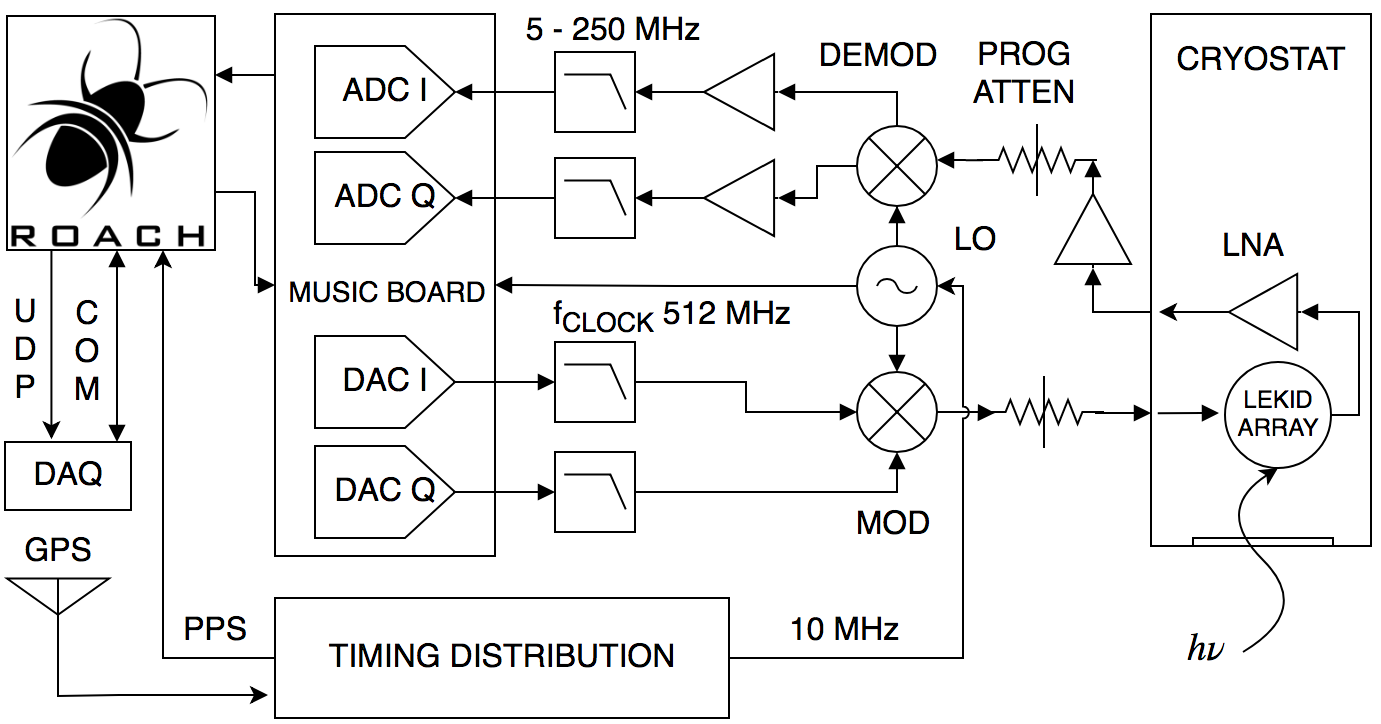
\includegraphics[width=\textwidth]{figures/readout/schematics/readoutHardwareSchematic}
\caption{A schematic of the BLAST-TNG readout electronics.}
\label{fig:hw schematic}
\end{sidewaysfigure}

The primary purpose of the IF electronics is to move the signals which are produced by the ROACH2 system between complex baseband (-256 to +256~MHz) and RF ($\sim$500--1100~MHz). Additionally, the signals require amplification after passing through the cryostat. The IF electronics in each readout slice include the following components\footnote{Not included in the list: Several meters of coaxial cable; many handfuls of SMA adaptors.}:

\begin{itemize}[nosep]
  \item Four 1--256~MHz anti-aliasing filters (custom-made at ASU, one each for the $I$ and $Q$ DACs and ADCs)
  \item One quadrature modulator (Polyphase Microwave AM0350A\footnote{Polyphase Microwave:\url{https://polyphasemicrowave.com/}})
  \item One quadrature demodulator (Polyphase Microwave AD0105B)
  \item Two Mini-Circuits\footnote{Mini-Circuits:\url{https://www.minicircuits.com/}} 6000-30 programmable attenuators (steppable between 0--30~dB in 0.25~dB increments)
  \item One room-temperature (RT) LNA, (custom-made at ASU)
  \item Two RT baseband amplifiers (custom-made at ASU, one each for $I$ and $Q$ on the downconversion side.)
  \item One dual-channel synthesizer (the Valon 5009)
  \item Two 1~GHz low-pass filters (Mini-Circuits VLF-1000+, used to filter out LO harmonics and at the RF input of the readout system).
  \item Two baluns (Mini-Circuits ADT2-1T+, used to convert the $I/Q$ modulator inputs from single-ended to differential.
\end{itemize}

\vspace{5mm}

A schematic of the digital and IF electronics signal processing chain is shown in Figure~\ref{fig:hw schematic}. For explanation purposes, the signal chain can be split into two chains which merge on one end at the ROACH2 system and at the cryostat (or detector arrays) at the other.

\textit{Upconversion chain:} Starting with the ROACH-2 board, the firmware generates a baseband probe tone comb containing the resonant frequencies of each detector in the LEKID array. The signal is output in quadrature ($I$ and $Q$) by the DACs, and low-pass filtered to remove higher-order Nyquist zones (see Section~\ref{tone comb}). The signal is then upconverted to RF in the quadrature modulator, which takes the $I/Q$ quadratures as differential inputs and outputs a single RF signal. To be input into the modulator, the $I$ and $Q$ signals are converted to differential using baluns\footnote{The baluns are not required for this particular modulator. However, it is desirable to have as little LO leakage as possible at the RF output. Using baluns reduces the LO leakage to $\sim$4~dB above the probe tone level. When driven single-ended, the LO is $\sim$20~dB above the probe tones.}. The upconverted signal is then attenuated by the output-side (relative to the ROACH2) programmable attenuator before being fed into the cryostat on a single coaxial cable. The cryostat contains several temperature stages between 300~K and 300~mK, where the detector arrays are kept. Each stage contains a fixed amount of attenuation whose purpose is to reduce the thermal load on the following (colder) stages. The total gain of the cryostat depends on fixed attenuation, cable losses and LNA gain. For BLAST-TNG, the cryogenic gain is $\sim$-20~dB. After being modulated by the LEKID detectors the signal is amplified by a cryogenic 6~K LNA\footnote{A SiGe LNA from Groppi Labs at ASU: \url{http://thz.asu.edu/products.html}} with 30--35~dB of gain, and sent back out of the cryostat.

\vspace{5mm}

\textit{Downconversion chain:} The downconversion chain begins when the signal exits the cryostat. It is first low-pass filtered (cut-off frequency at $\sim$1~GHz) to remove any signal above $\sim$1~GHz which was amplified by the high gain of the cryogenic LNA. The signal then enters a second-stage amplifier, which for BLAST-TNG is a RT LNA which has been modified to operate on  5~VDC. The second-stage amplifier is followed by the programmable input attenuator, which feeds the demodulator. The demodulator splits the signal back into quadratures, which are passed through a third-stage of amplification that provides $\sim$20~dB of gain. The purpose of the third-stage amplifiers is to ensure that enough signal power enters the ADC when the probe tones are on resonance. The amplified quadratures are then low-pass filtered through the second pair of 1--256~MHz anti-aliasing filters, and input to the $I$ and $Q$ ADCs.

The power dissipation for each of the active IF components is listed in Table~\ref{tab:if power budget}. Their total power dissipation is $\approx$~19~W. Adding this value to the $\approx$~45~W which are dissipated by the digital electronics (Section~\ref{digital electronics}) gives a total power dissipation of $\approx$~66~W. This per-readout slice power dissipation is within acceptable range of the BLAST-TNG power requirement of $\lesssim$60~W per slice.

\begin{table}[!htbp]
\centering
\begin{tabular}{@{}lllll@{}}
\dtoprule
Part & Quantity & Volts (V) & Current (mA) & Total Power (W) \\ \midrule
Valon 5009 & 1 & 6 & 600 & 3.6 \\
RUDAT 6000-30 & 2 & 5 & 60 & 6 \\
Polyphase AM0350A & 1 & +5/-5 & 250/30 & 2.75 \\
Polyphase AD0540B & 1 & +5/-5 & 290/50 & 3.95 \\
RT LNA & 1 & 5 & 30 & 1.5 \\
Baseband RT Amps & 2 & 5 & 145 & 1.45 \\
 &  &  &  & 18.94 \\ \dbottomrule
\end{tabular}
\caption[~The power dissipation for the IF electronics used in each BLAST-TNG readout slice]{The power dissipation for the IF electronics used in each BLAST-TNG readout slice}
\label{tab:if power budget}
\end{table}

\subsection{Readout Electronics for the Balloon Platform: The BLAST-TNG ROACH2 Motel}

The ROACH2 Motel, shown fully assembled in Figure~\ref{fig:roach sunset}, is a custom aluminum (Al) enclosure that houses the set of five ROACH2 readout slices, including their digital and IF electronic components. The electronics for each readout slice are mounted to 1/4$\arcsec$ backing plates, which are stacked side by side between two 5/8$\arcsec$ thick Al side panels. To allow for continuous operation at float altitude ($\sim$35~km), where fans have little effect due to the lack of atmosphere, the enclosure itself must provide a thermal link to the inner frame of the balloon gondola to enable the heat generated by the electronics to dissipate and radiate to space. Heat from each slice's backing plate flows through the two Al side panels and into two 8$\arcsec$ $\times$ 5$\arcsec$ $\times$ 1/4$\arcsec$ right angle brackets which secure the enclosure to the inner frame of the gondola (see Figure~\ref{fig:mounting roaches}). All contact joints between metal components within the enclosure are coated with non-conductive thermal joint compound to increase their thermal conductivity.

% Sunset glory
\begin{figure}[!htbp]
\centering
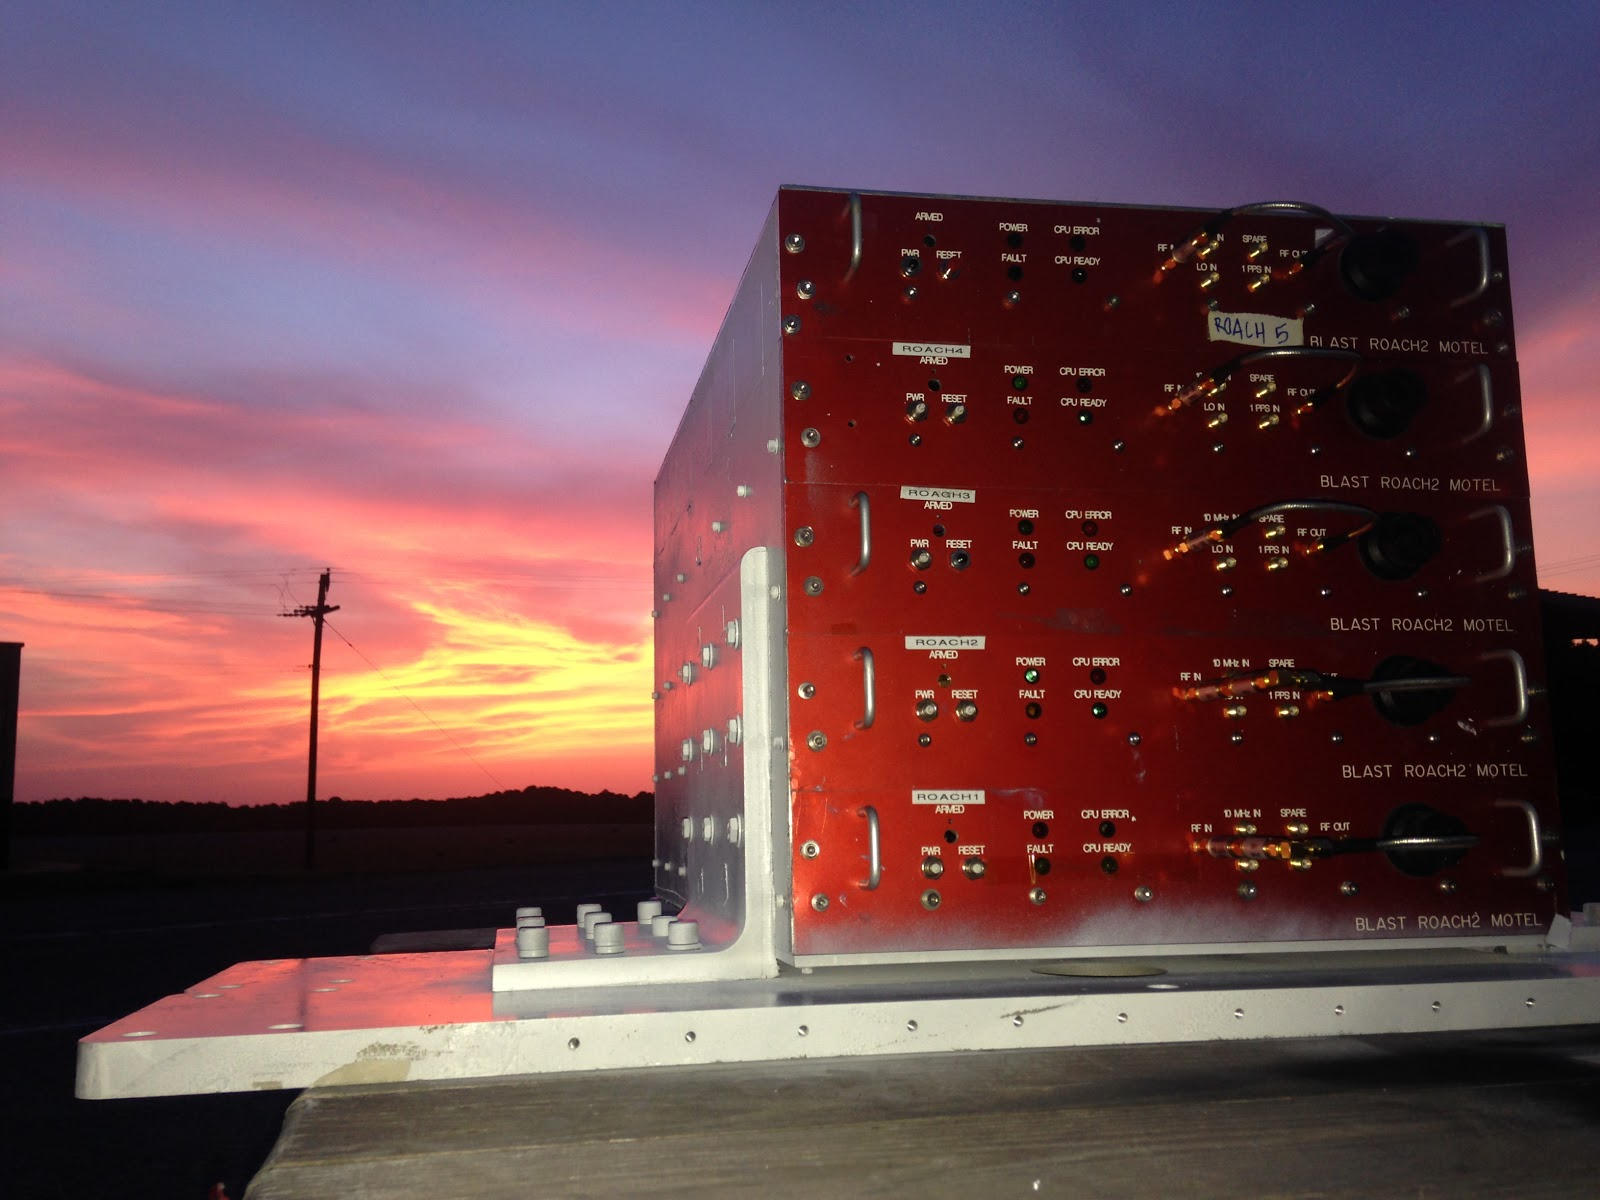
\includegraphics[width=\textwidth]{figures/readout/hardware/roach_sunset}
\caption{The BLAST-TNG ROACH2 Motel, fully assembled and taking in the sunset in Palestine, Texas, USA.}
\label{fig:roach sunset}
\end{figure}

Each of the electronics used in the BLAST-TNG detector readout are rated for operation to at least 85$^\degree$C. In order to stay within their operational temperature limits, the FPGA, PPC and ADCs must be well heat sunk to the inner plates of the enclosure, which in turn must have their own path for dissipating heat. The ROACH2's Xilinx Virtex-6 FPGA is by far the largest producer of heat in each electronics slice. To address this, a copper assembly containing two 5~mm diameter water filled, sintered copper heat pipes\footnote{Enertron Inc:\url{https://www.enertron-inc.com/}} are mounted directly on top of the FPGA chips. The heat pipes are soldered into the heat sink assemblies using bismuth tin (BiSn) solder paste. BiSn is used because its relatively low melting point of 138$^{\degree}$C allows it to liquify during fabrication without damaging the heat pipes.

% Installing ROACH2 Motel
\begin{figure}[!htbp]
\centering
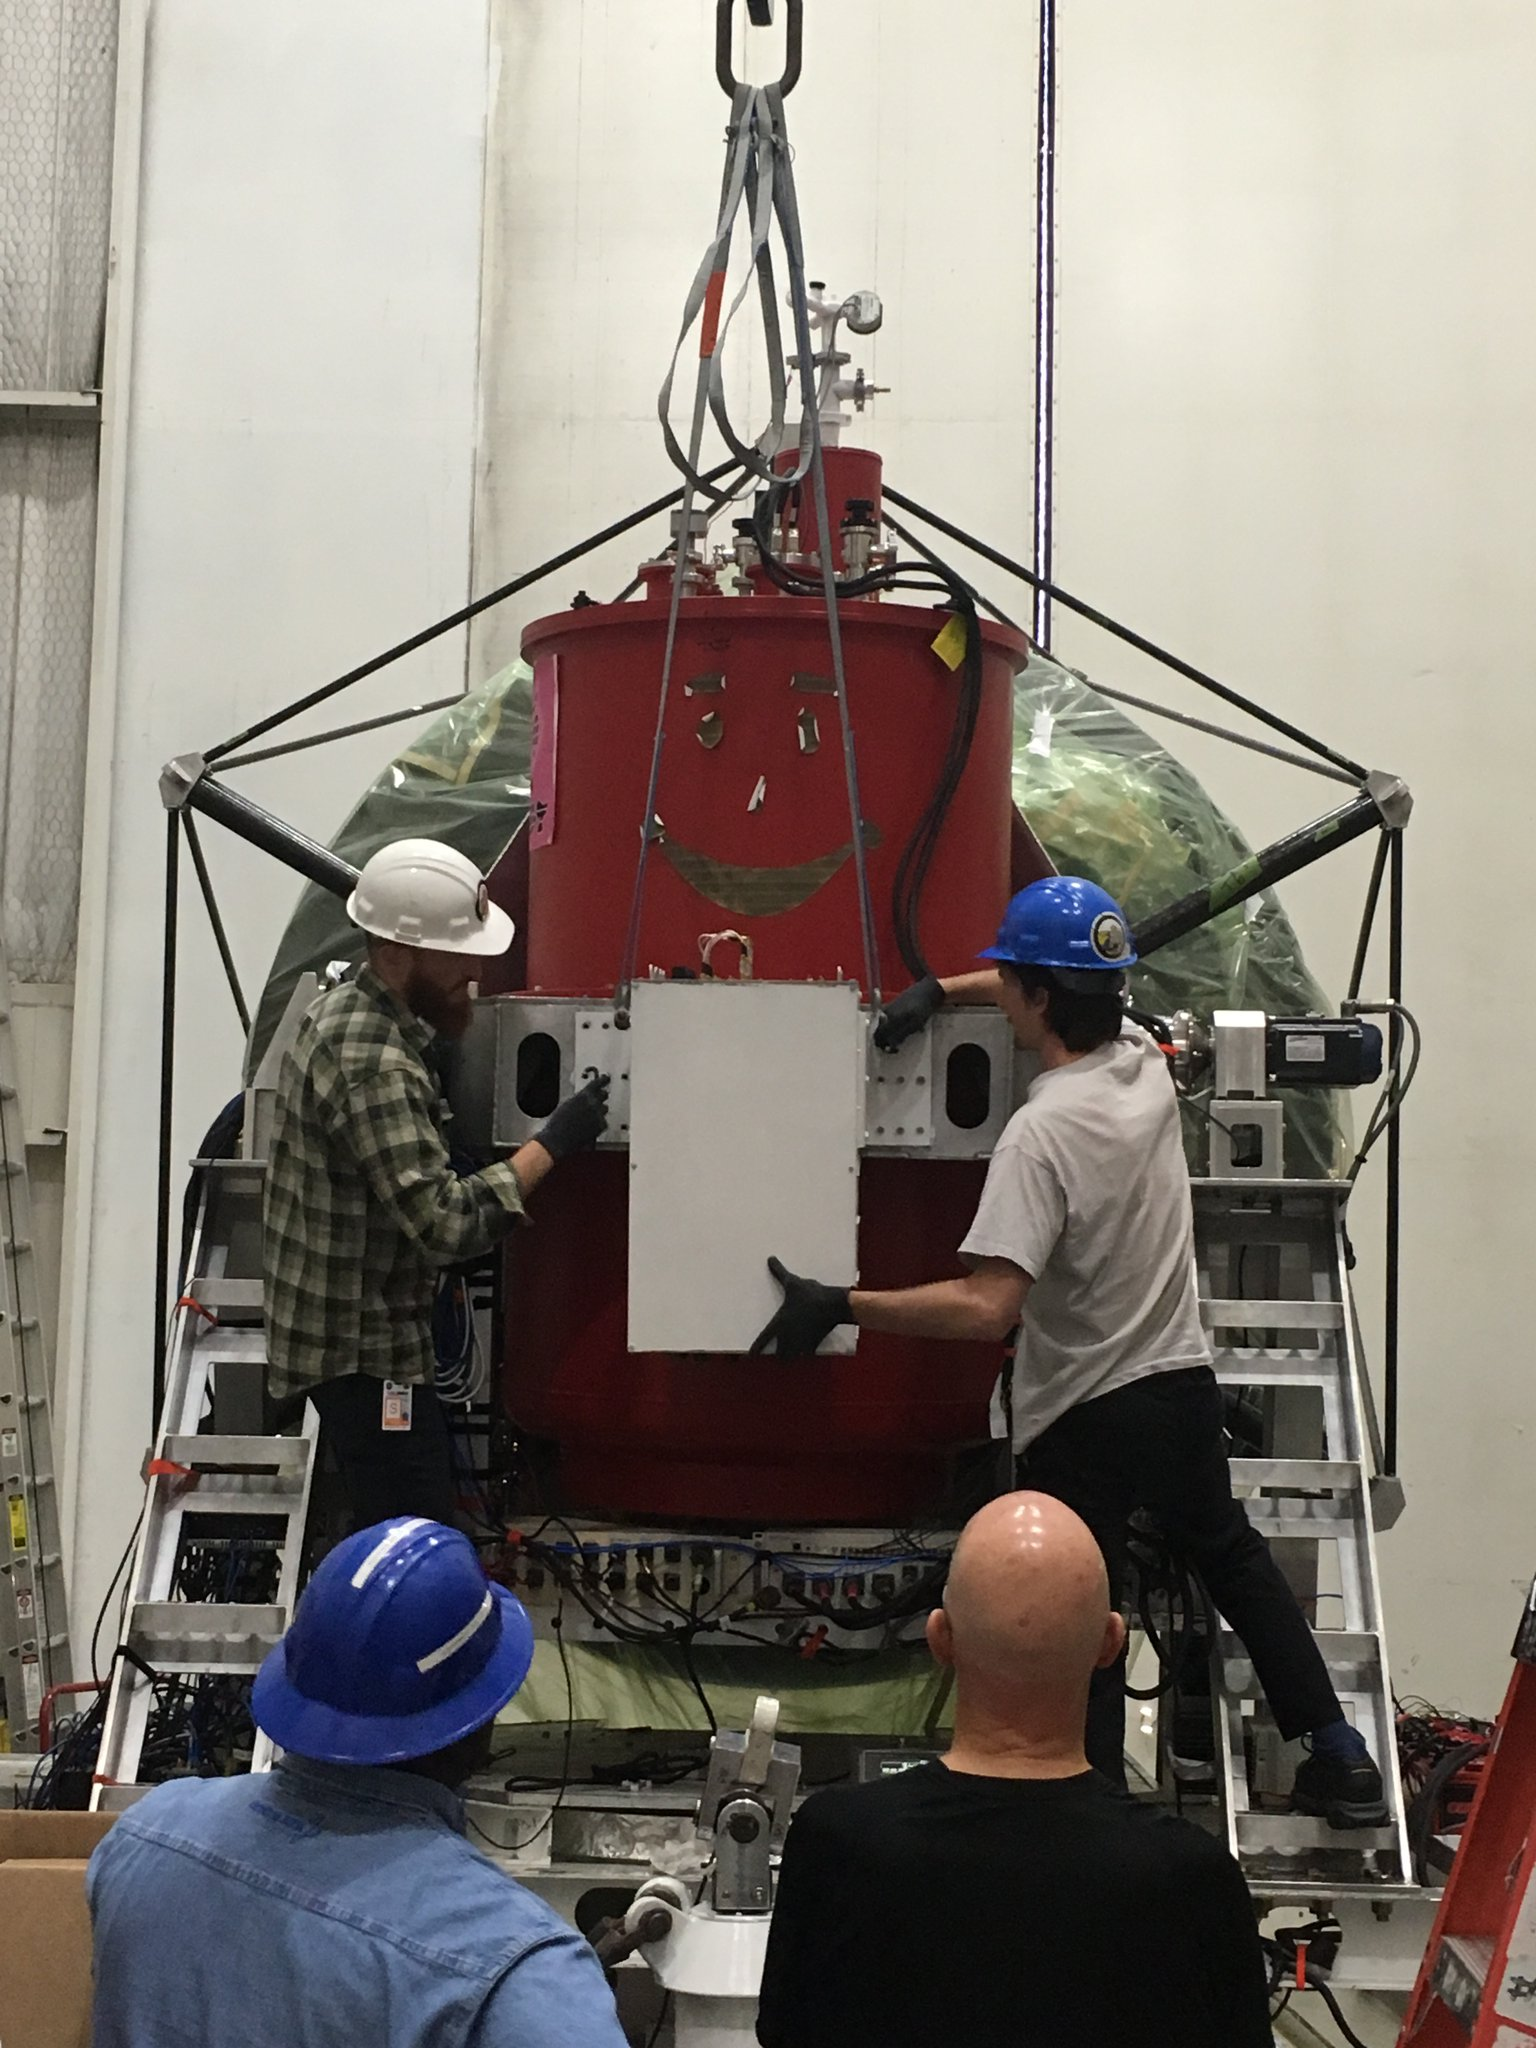
\includegraphics[width=0.8\textwidth]{figures/readout/hardware/installing_roaches}
\caption{The `Roach Boys' installing the Roach2 Motel on the BLAST-TNG gondola in Palestine, Texas, USA (July, 2018).}
\label{fig:mounting roaches}
\end{figure}

Besides the FPGA, the two most sensitive components are the PPC and ADCs. The PPC is heat-sunk to the FPGA's heat pipe assembly using two smaller copper heat pipes, and the the ADCs are heat strapped directly to the 1/4$\arcsec$ Al backing plates using 10 AWG copper wires which are secured to the chips using non-conductive thermal epoxy. The DACs, which run cooler than the ADCs, are connected to the backing plate by a single 14~AWG copper wire. The Raspberry Pi 3 boards are mounted to Al plates which are secured to the backing plate of each slice. The IF electronics are mounted to the same backing plate as the digital electronics.

During operation of the system, the temperature of the FPGAs and PPCs is logged via temperature sensors which are secured to the heat sinking assemblies of each device. The CPU temperatures of each Raspberry Pi 3 board are also logged.

Power suppy and input and output signals are routed through the front and back panels of the ROACH2 Motel. Each slice's front panel includes SMA input ports for: A 10~MHz reference, a PPS signal, an (optional) external LO, RF input and output, and a spare input. The back panel of each slice contains a 4-pin military connector which receives 28~VDC from the balloon gondola’s power distribution system. This voltage is distributed to several Vicor\footnote{Vicor:\url{http://www.vicorpower.com}} DC-DC converters which are mounted to the enclosure's backing plate. The DC converters supply $\pm$5, 6 and 12~VDC to the IF electronics. The back panels also contain Ethernet port for communicating with the PPC, FPGA, and Raspberry Pi 3, as well as a USB port for interfacing directly with the Linux OS (BORPH) which runs on the PPC.

Figure~\ref{fig:if slice} is an annotated photograph of one of the five BLAST-TNG ROACH2 slices, taken during the 2018-2019 Antarctic campaign. Critical components are labeled with numbers. These are: 1) ROACH2 board 2) FPGA heat pipe assembly 3) Raspbery Pi 3 4) MUSIC DAC/ADC board 5) anti-aliasing filters 6) programmable attenuators 7) demodulator 8) modulator 9) second-stage LNA (not visible) 10) Valon synthesizer (not visible). A view of the fully assembled motel is shown in Figure~\ref{fig:top roach}. The outside of the enclosure is painted white to increase its albedo. Ethernet ports for the FPGA and PPC can be seen forming two columns that run along the back panel. The power distribution for the exposed ROACH2 slice is routed through a D-sub connector at the lower left corner of the image.

% Installing ROACH2 Motel
\begin{sidewaysfigure}[!htbp]
\centering
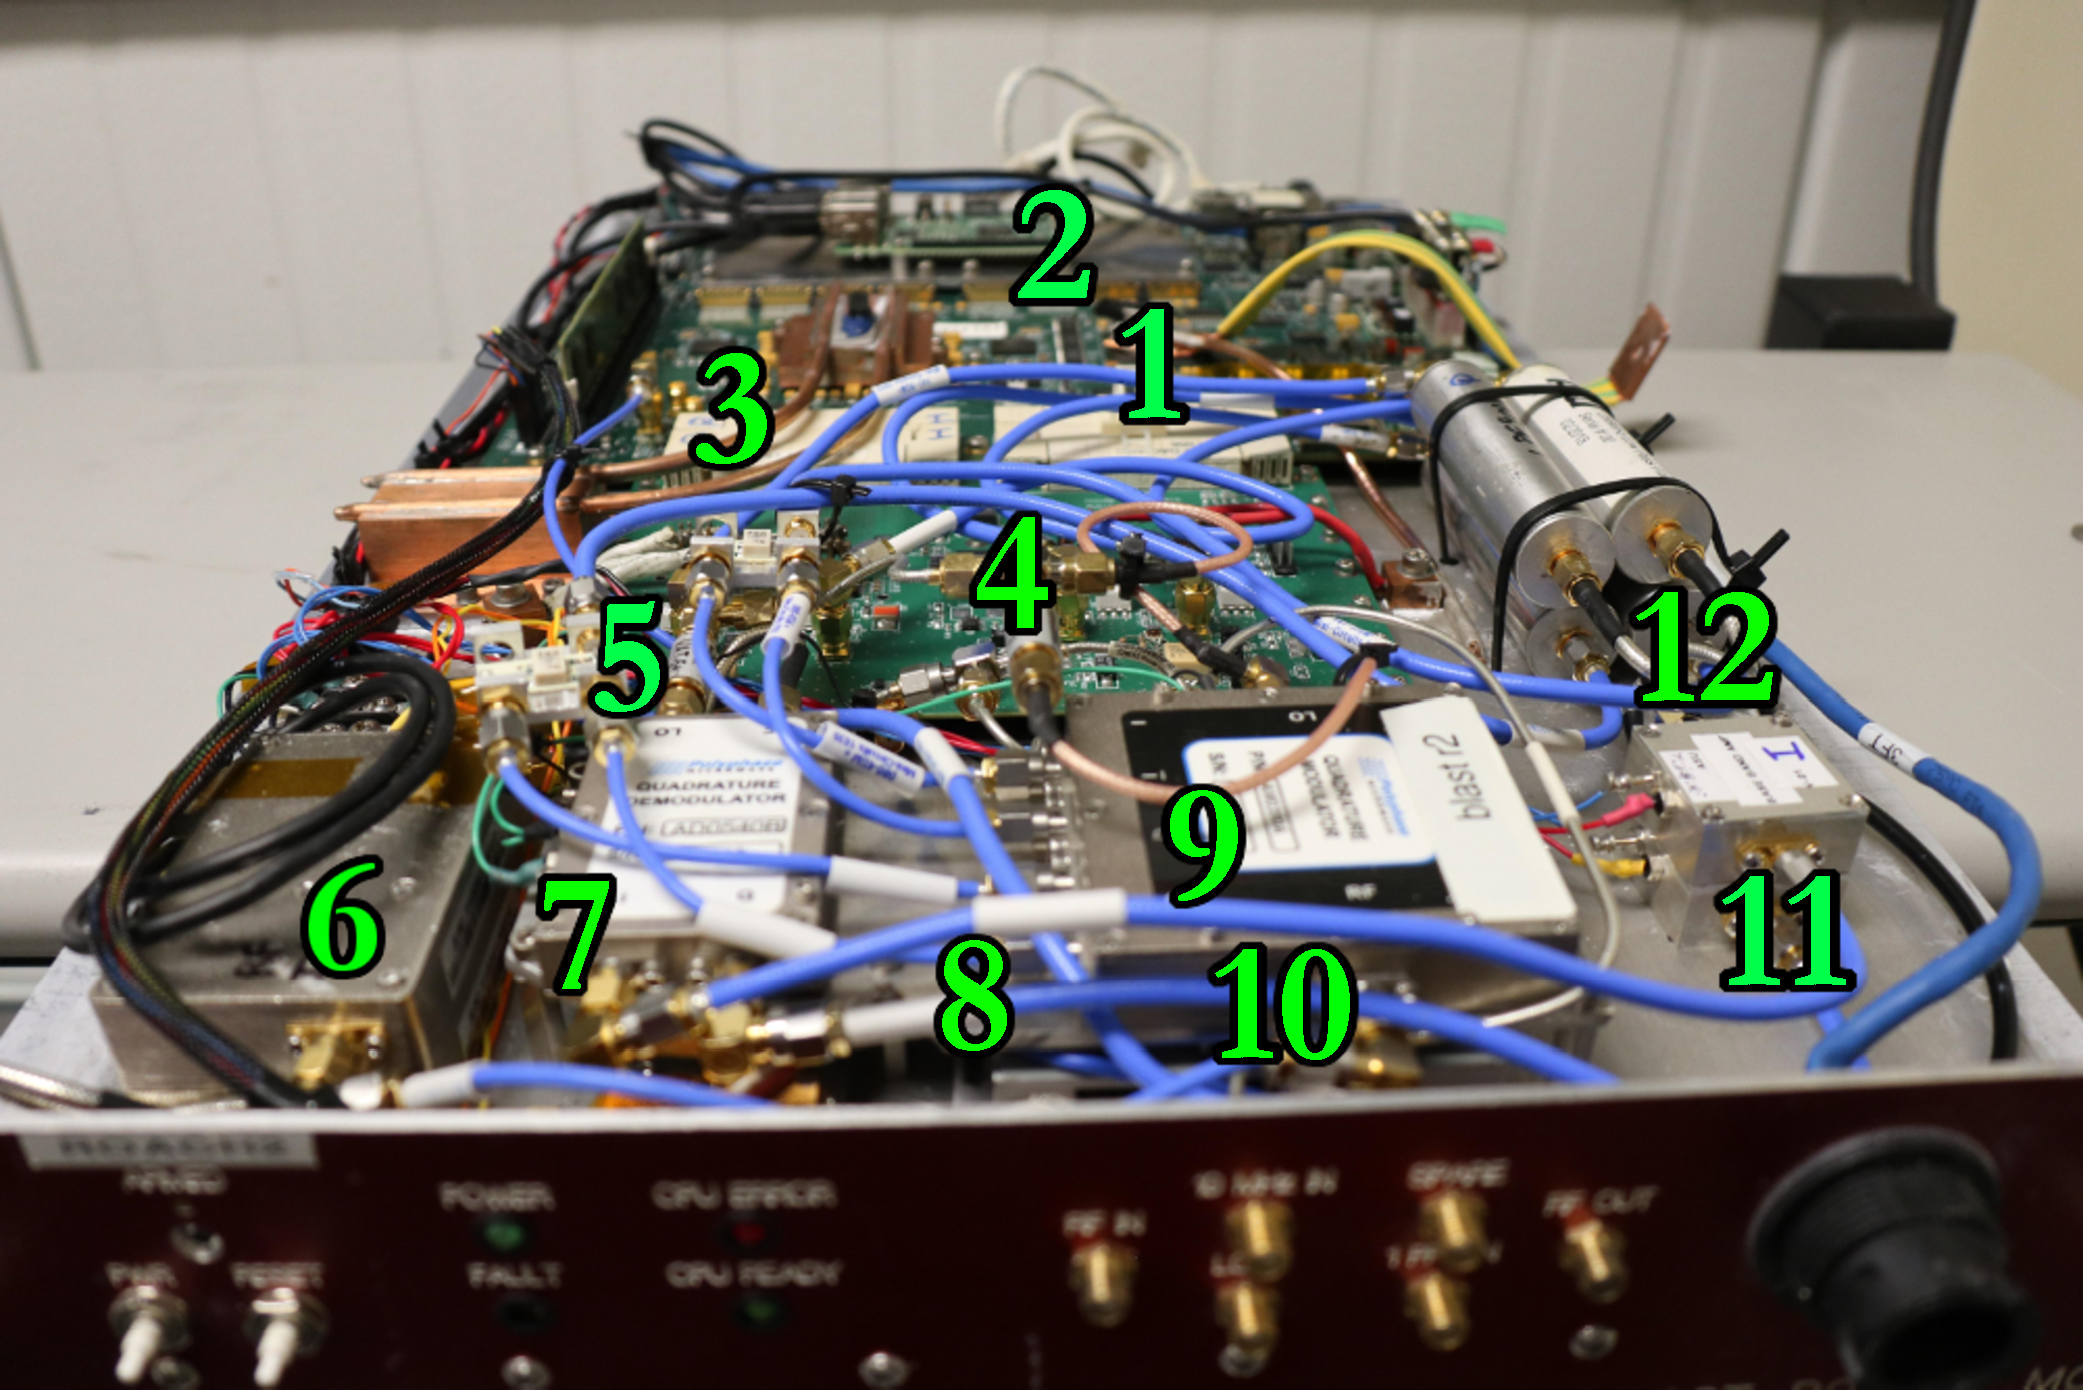
\includegraphics[width=\textwidth]{figures/readout/hardware/roach_slice_annotated}
\caption[~An annotated photograph of one of the five BLAST-TNG ROACH2 electronics slices.]{An annotated photograph of one of the five BLAST-TNG ROACH2 electronics slices. These are: 1) ROACH2 board 2) Raspberry Pi 3 3) FPGA heat pipe assembly 4) MUSIC DAC/ADC board 5) baluns 6) programmable attenuators 7) demodulator 8) RT LNA (not visible) 9) modulator 10) Valon synthesizer (not visible) 11) third-stage amplifiers 12) anti-aliasing filter stack.}
\label{fig:if slice}
\end{sidewaysfigure}

% Lid open
\begin{figure}[!htbp]
\centering
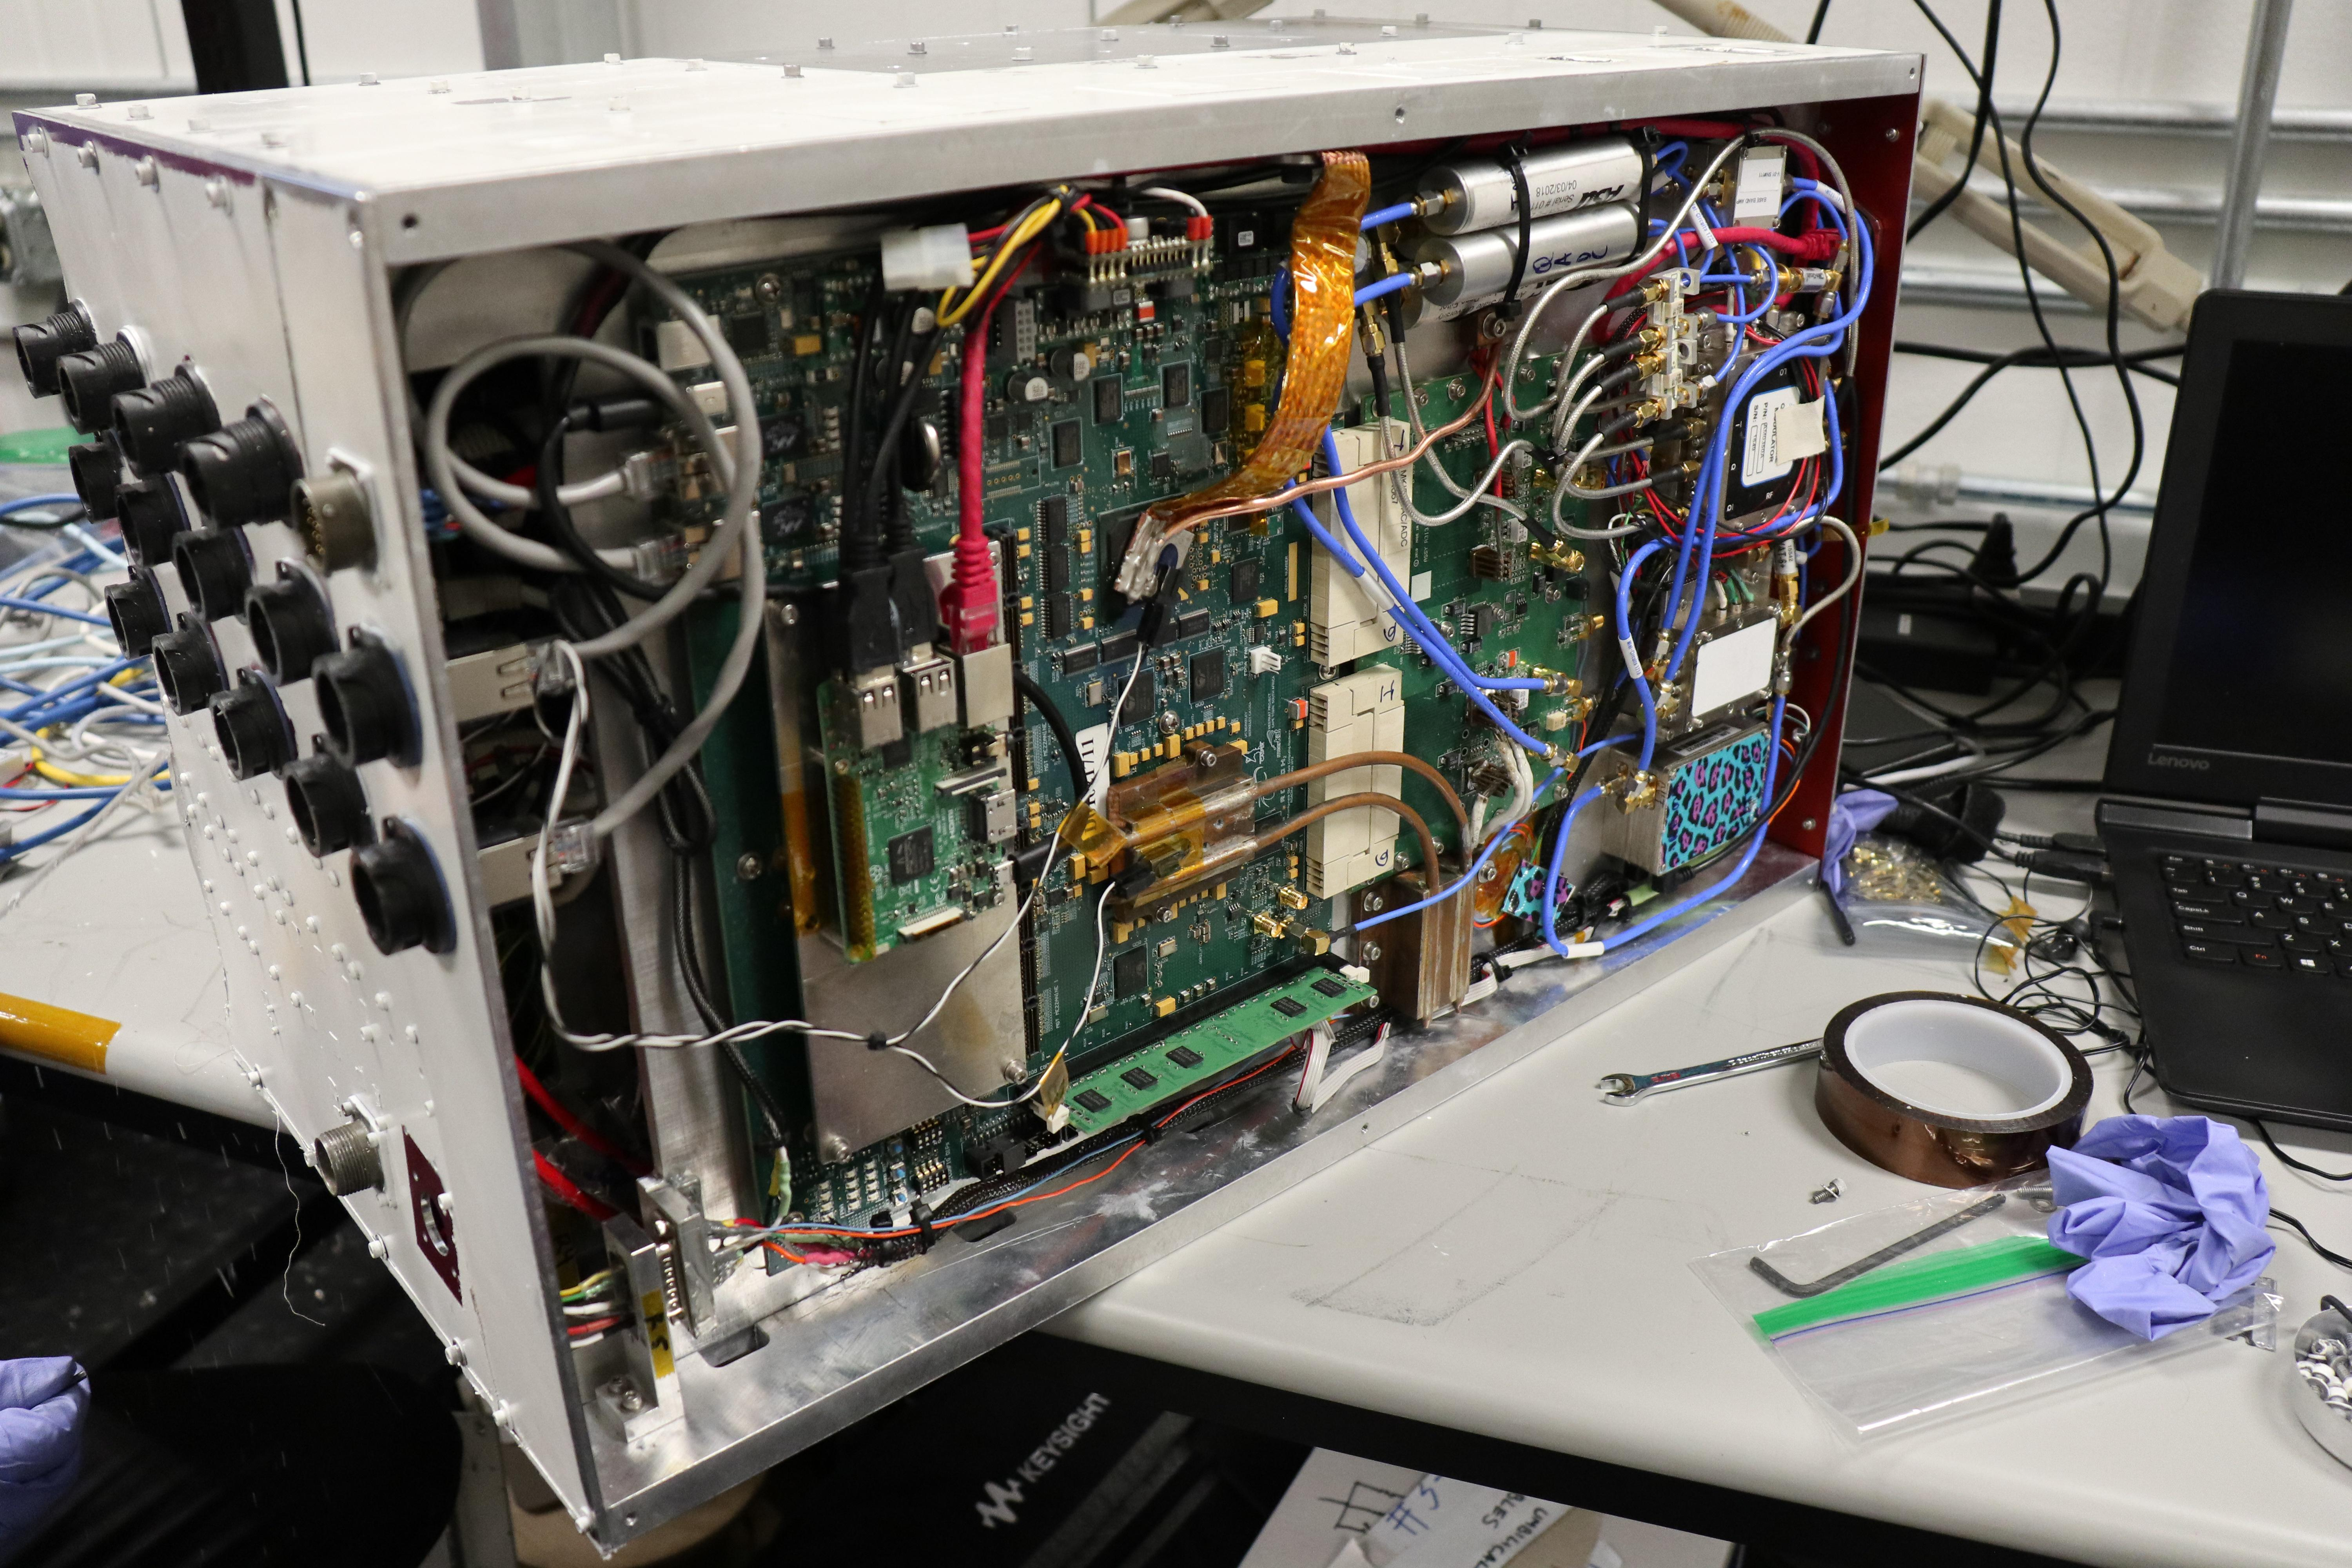
\includegraphics[width=\textwidth]{figures/readout/hardware/roach_motel_open}
\caption[~A top view of the BLAST-TNG ROACH2 Motel, with the lid removed.]{A top view of the BLAST-TNG ROACH2 Motel, with the lid removed.}
\label{fig:top roach}
\end{figure}

\begin{comment}
\begin{figure}[!htbp]
\centering
\includegraphics[width=0.8\textwidth]{figures/readout/minicircuitsLPFcomp_crop}
\caption{Comparison of the simulated S21 (ASU, red), measured S21 (ASU, black) and measured S21 (Minicircuits, blue).}
\label{fig:lpf comp}
\end{figure}

\begin{figure}[!htbp]
\centering
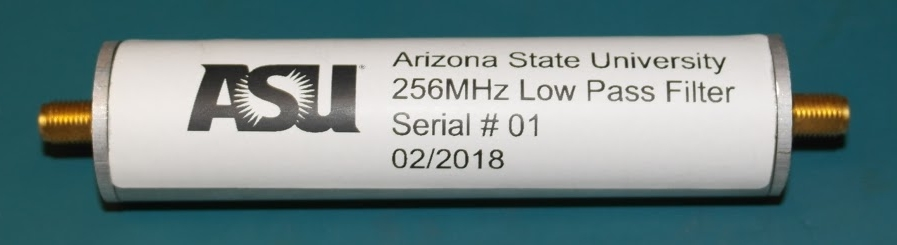
\includegraphics[width=0.8\textwidth]{figures/readout/lpf_tube}
\caption{Comparison of the simulated S21 (ASU, red), measured S21 (ASU, black) and measured S21 (Minicircuits, blue).}
\label{fig:lpf}
\end{figure}

\begin{figure}[!htbp]
\centering
\includegraphics[width=0.8\textwidth]{figures/readout/activeFilterbox_crop}
\caption{Comparison of the simulated S21 (ASU, red), measured S21 (ASU, black) and measured S21 (Minicircuits, blue).}
\label{fig:activeFilter}
\end{figure}

\begin{figure}[!htbp]
\centering
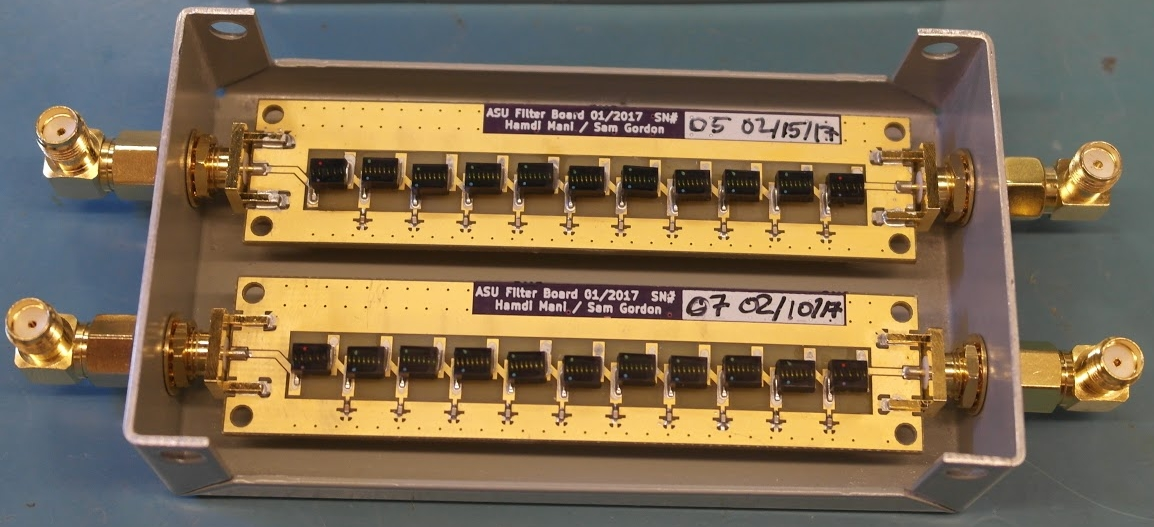
\includegraphics[width=0.8\textwidth]{figures/readout/dac_lpf_crop}
\caption{Comparison of the simulated S21 (ASU, red), measured S21 (ASU, black) and measured S21 (Minicircuits, blue).}
\label{fig:dacLPF}
\end{figure}

\begin{figure}[!htbp]
\centering
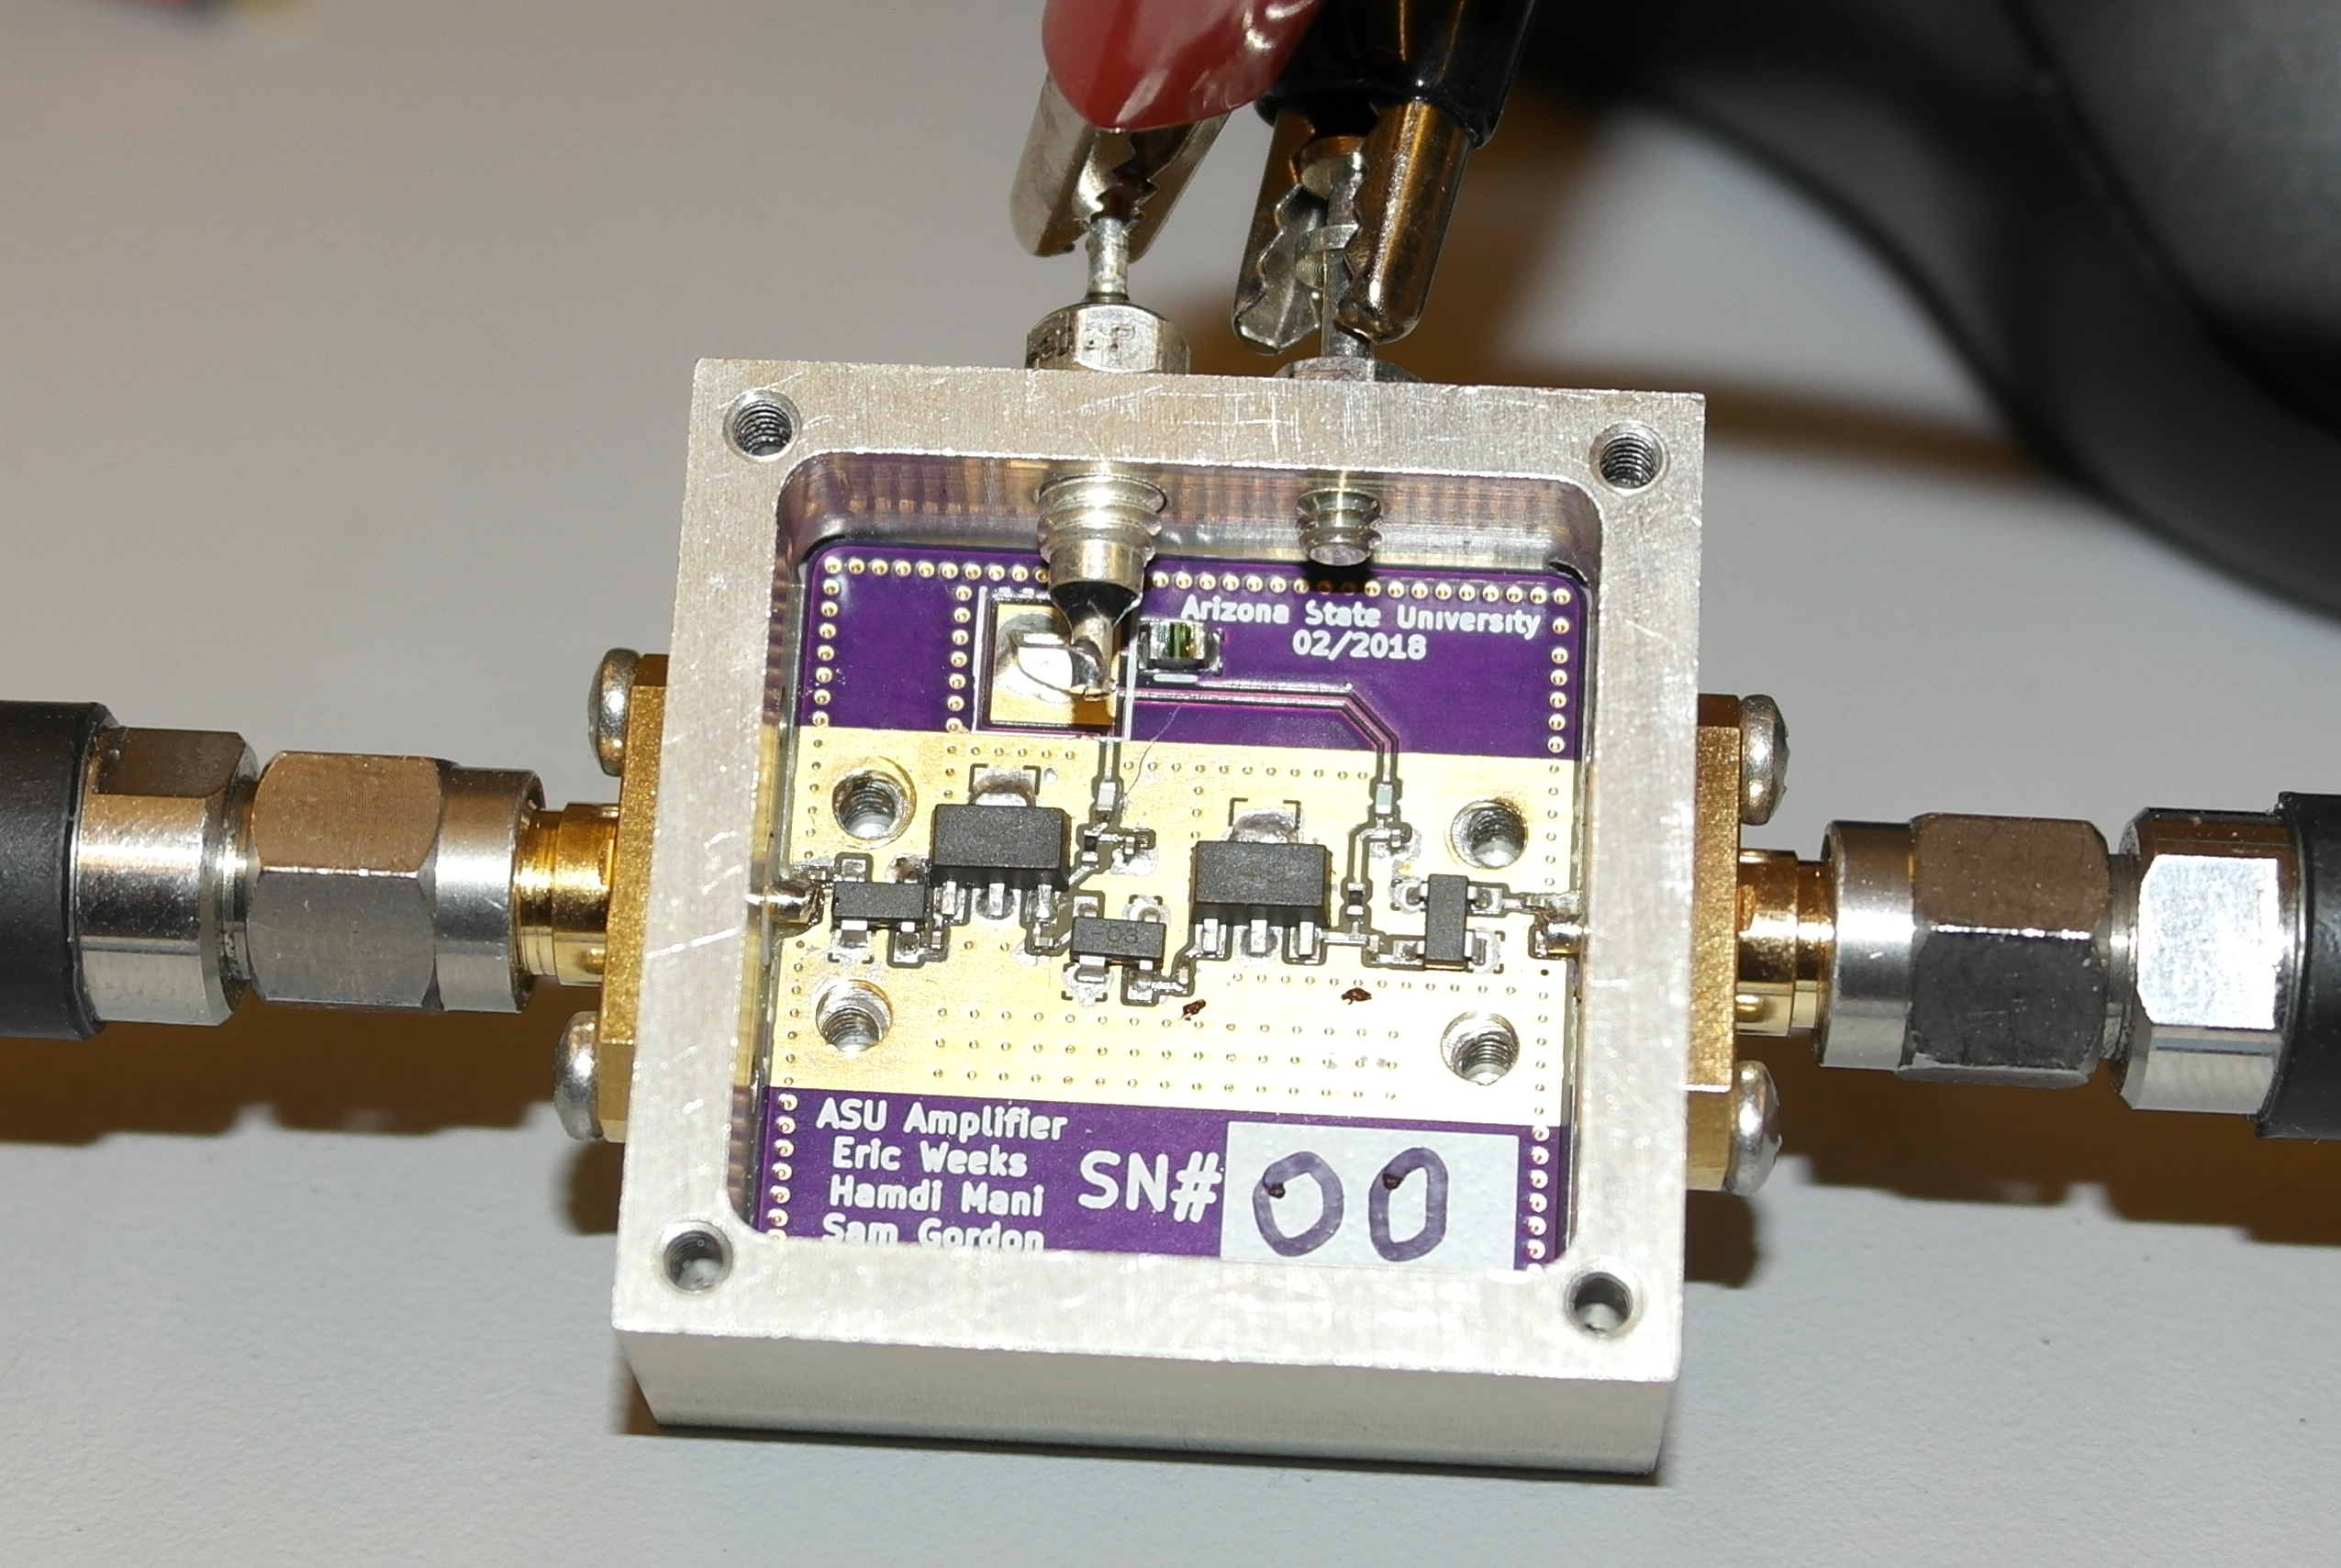
\includegraphics[width=0.8\textwidth]{figures/readout/bb_amp_00_crop}
\caption{Comparison of the simulated S21 (ASU, red), measured S21 (ASU, black) and measured S21 (Minicircuits, blue).}
\label{fig:bb_amp_00}
\end{figure}
\end{comment}

\section{ROACH2 Firmware Overview}\label{firmware}

In this section we describe in detail the DSP which is performed in the FPGA firmware. The firmware is written using the MATLAB\footnote{Mathworks:\url{https://www.mathworks.com/}} / Simulink\footnote{Mathworks} / System Generator\footnote{Xilinx ISE 14.7 Design Suite} / EDK\footnote{Xilinx Embedded Development Kit} (MSSGE) Toolflow developed by the CASPER collaboration. CASPER `snap' blocks allow for pre-specified amounts of data from the data stream to be saved in block RAM (BRAM) on the FPGA at key points in the DSP chain. This data can then be converted into figures of merit to be used for making real-time adjustments to either the RF electronics or baseband frequency combs. Critical parameters, including the readout bandwidth, may be adjusted during operation using software inputs.

The DSP chain performs several synthesis and analysis functions, which are described sequentially in the sections below. A block diagram of the DSP chain is shown in Figure~\ref{fig:DSP schematic}.

% DSP flow
\begin{sidewaysfigure}[!p]
\centering
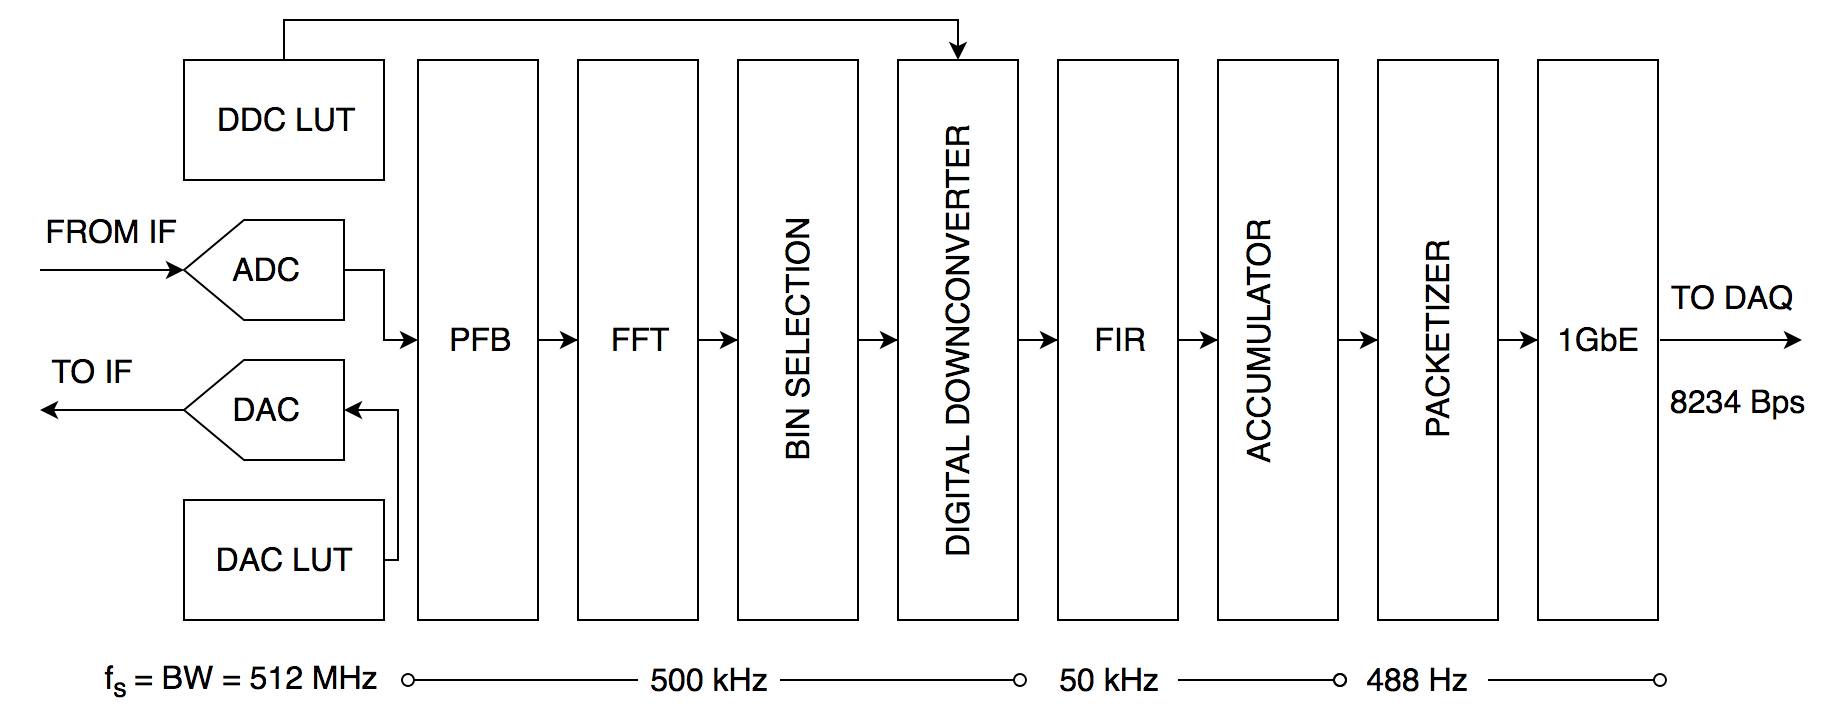
\includegraphics[width=\textwidth]{figures/readout/schematics/readoutDSPschematic}
\caption{A schematic of the firmware DSP chain.}
\label{fig:DSP schematic}
\end{sidewaysfigure}

\subsection{Tone Comb Synthesis}\label{tone comb}

The DSP chain begins with the synthesis of the DAC probe tone and DDC tone look-up-tables (LUTs). The DDC tones are used to digitally downconvert the output timestreams of the PFB-FFT (see Section~\ref{ddc}), and the DAC probe tones circulate between the readout system and the LEKID arrays throughout an observation. If the resonator frequencies are not known, they can be discovered using the channel identification technique described in Section \ref{KID-finding}. In the following, we assume that the LEKID resonant frequencies ($f_{res}$) are already known.

The time domain waveform of the DAC probe tone is synthesized in software (\texttt{Python/C/C++}) by assembling a dummy spectrum in the frequecy domain, and then taking its inverse-Fourier transfrom (IFT). In the dummy spectrum, each probe tone is represented by an amplitude $A$ and unique phase $\phi$. During an observation, the probe tone amplitudes are set to unique values corresponding to the specific tone power requirements of the detectors (including a global transfer function correction to correct for the ROACH2-output side IF electronics, described in Section~\ref{TRF}). In the examples which are provided in the following, the tone amplitudes are normalized to their maximum allowable value, which is 32767 analog-digital units (ADU). At the DAC output, this level corresponds to $V_{pp} \simeq 1.4$~V.

The phases of the probe tones are chosen from a normal distribution. This produces a near-optimal CF for a multitone comb with an arbitrary number of tones (\citet{boyd1986multitone}). The tone frequencies occupy the complex baseband bandwidth of the ROACH2/MUSIC board system, which spans from -256 to +256~MHz (for a good explanation of negative frequency, see \citet{lyons2004understanding}). The tone frequencies are rounded to increments of the final channelizer bandwidth of 488.28125~Hz.

The DDC tones are computed in a similar fashion as the DAC tones, although their frequencies correspond to the difference between the DAC probe tone frequencies and the center frequencies $f_{k}$ of their firmware FFT bins. For a given FFT bin index $k$, $f_{k} = kf_{s}/N_{FFT}$. The frequency of the DDC tone corresponding to a probe tone at frequency $f_{pr}$ which is located in bin $k$ is therefore $f_{k,DDC} = f_{pr} - f_{k}$. The sampling frequency for the DDC LUT is the PFB-FFT output frequency, $f_{FFT} = 500$~kHz.

Once synthesized in software, the DAC and DDC comb LUTs are uploaded to the ROACH2 board, where they occupy two of the ROACH2's four quad-data-rate (QDR) SRAM chips\footnote{Cypress, CY7C2565KV18}, hereafter designated QDR$_{I}$ and QDR$ _{Q}$. Each LUT contains 2$^{21}$ signed 16-bit time ordered samples.

The QDR is logically accessed as 2$^{19}$ addresses $\times$ 16-B. The KATCP protocol is used to upload the LUT data to QDR RAM. To facilitate uploading the two LUTs to each QDR, the $I$ and $Q$ components are interwoven into two separate LUTs (LUT$_{I}$, LUT$_{Q}$) of 2$^{22}$ time ordered samples each (this is based on the method used by \citet{mchugh2012readout}). For example, the order of samples contained within LUT$_{I}$ is:

\begin{equation} I_{DAC}^{1}, I_{DAC}^{0}, I_{DDC}^{1},I_{DDC}^{0}, ... , I_{DAC}^{n}, I_{DAC}^{n -1 }, I_{DDC}^{n}, I_{DDC}^{n - 1} \end{equation}
where superscripts refer to even and odd numbered samples, and each value is 16-bit wide.

After the LUTs have been uploaded to the QDRs, they are read from the QDR buffers, sliced into their original 16-bit values and re-cast as fixed-point 16.15 values\footnote{In this fixed-point notation, the first number represents the total bit width, with the second number being the radix point. All numbers in this notation are assumed to be signed unless otherwise noted.}. On each clock cycle, four consecutive samples are read out from QDR$_{I}$ (QDR$_{Q}$): $I_{DAC}^{1}, I_{DAC}^{0}, I_{DDC}^{1}, I_{DDC}^{0}$ (same for $Q$).

The DDC LUT samples are sent directly to the DDC section of the firmware, while the DAC LUT samples are input to the MUSIC board DAC gateware. Since the DACs are clocked at twice the rate of the FPGAs, two consecutive samples (e.g., $I_{DAC}^{1}, I_{DAC}^{0})$ are processed on each FPGA clock cycle. To ensure proper synchronization of each quadrature component, the DAC is synchronized by a pulse which simultaneously resets the QDR address counter.

Because the DAC waveforms are reconstructed using a zero-order hold (ZOH), the frequency response of the waveform is a sinc function: $\mathcal{X}(f) = \left|{\mathrm{sinc}}(\pi f/f_{s}) \right|$. The sinc response produces two effects which must be considered individually. The first effect is a roll-off of $\sim$6~dB between the center of the band and the edge of the first Nyquist zone, at $f_{FPGA} = 256$~MHz. This roll-off is dealt with by applying an inverse transfer function correction to the probe tone amplitudes.

The second consequence of the ZOH is that several higher order Nyquist zones are output by the DAC, which must be removed using high-order low-pass filters. Figure~\ref{fig:dac sim} shows the measured output of one DAC for a tone comb comprised of 1000 evenly spaced tones, ranging from -245 -- +245~MHz. The blue trace is the unfiltered frequency response out to 1.5~GHz. The power in the second Nyquist zone ($f_{s}$--$\frac{3}{2}f_{s}$) is $\sim$10~dB below the peak at $f \simeq 250$~MHz. The orange trace shows the simulated sinc response. The simulation is a good match the first Nyquist zone, but does not taper off at higher zones (no frequency dependent attenuation factor was included in the simulation). The red trace shows the DAC output after the application of the anti-aliasing filters, which cut off at $\sim$245~MHz.

\begin{figure}[!htbp]
\centering
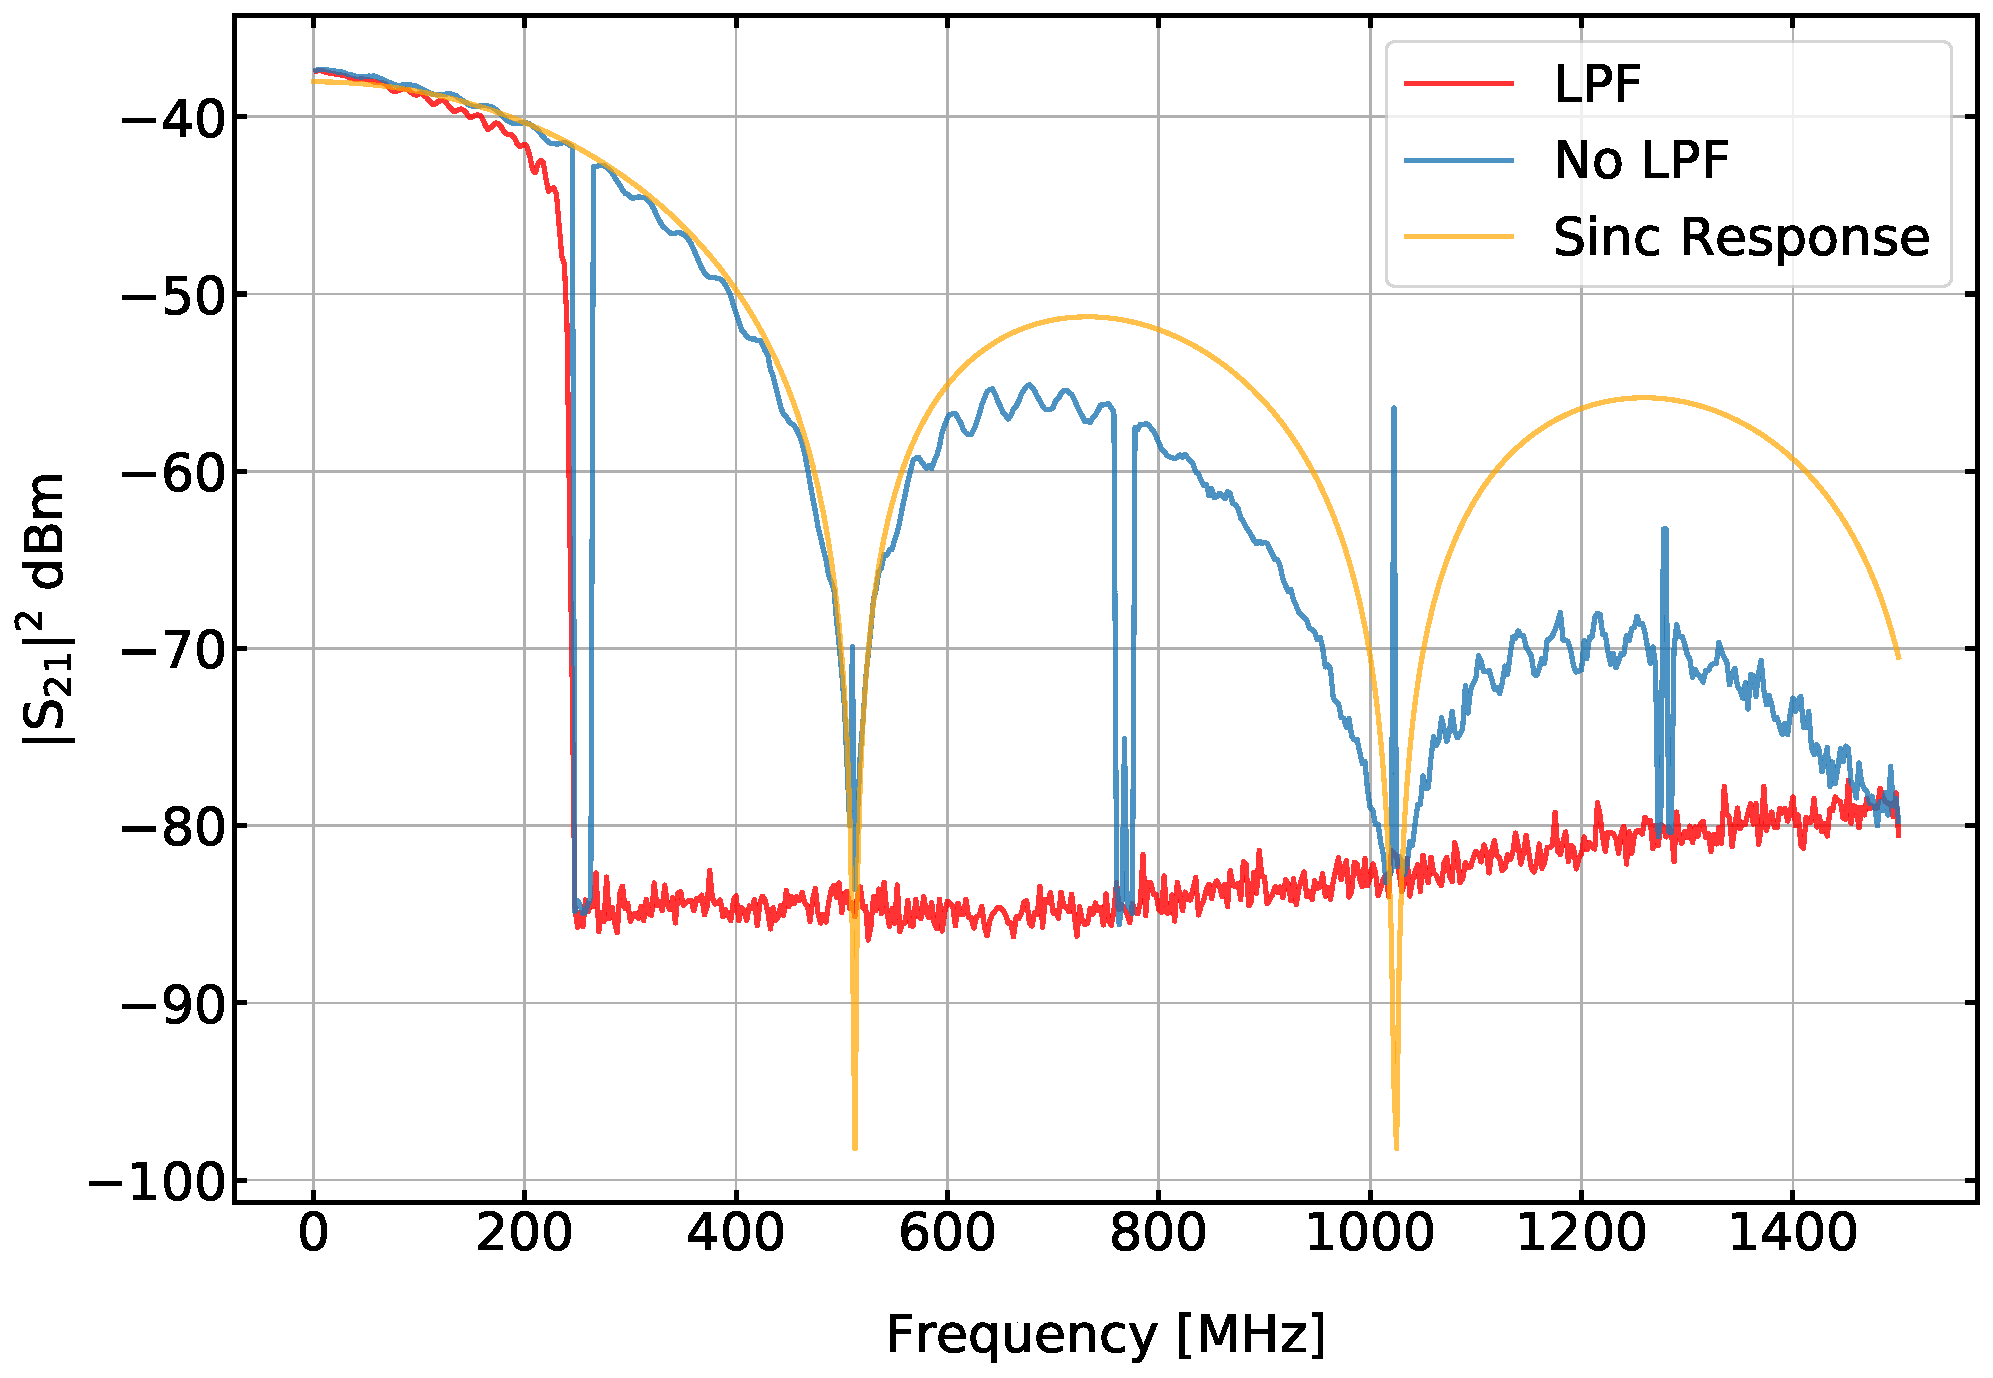
\includegraphics[width=\textwidth]{figures/readout/sim/dac_comp}
\caption[~The DAC frequency response (measured and simulated), with and without anti-aliasing filters.]{The DAC frequency response for a multitone probe comb with $N = 1000$, showing the unfiltered (blue), simulated (orange) and measured filtered (red) response out to 1.5~GHz.}
\label{fig:dac sim}
\end{figure}

\subsection{Digitization}\label{digitization}

After the tone comb has been upconverted by the IF electronics, passed through the detector arrays, and once again downconverted to complex baseband, the $I$ and $Q$ signals are digitized by two independent ADCs which share the same clock source as the DACs. Each ADC outputs two consecutive time samples per FPGA clock cycle: I$_{ADC}^{1}$, I$_{ADC}^{0}$ (Q$_{ADC}^{1}$, Q$_{ADC}^{0}$). The time ordered $I/Q$ pairs are concatenated and sent to the first stage of channelization, which is the PFB-FFT. CASPER snap blocks are utilized at this stage to store some of the ADC timestream in BRAM, which can be downloaded to the DAQ at any time in order to calculate $V_{\mathrm{RMS}}$ at the ADC input for both $I$ and $Q$. The ADCs have a full-scale input range of 1.1~V, which corresponds to a maximum allowable input power of 10.8~dBm.

Figure~\ref{fig:adc} shows 2,000 samples of the digitized timestream of a single tone at $f_{pr} = 50.0125$~MHz, as well as for a tone comb with $N_{tones} = 1000$ with evenly spaced frequencies. The power in the single tone has been attenuated using the output attenuator inside the IF electronics, to avoid saturating the ADCs. Because the phases of the multitone comb are randomized, the peak power in the comb scales as $p_{max} \propto \sqrt{N_{\mathrm{tones}}}$. During an observation, the IF attenuators are adjusted to keep the RMS voltage of the tone comb to below $\approx$~100~mV. This ensures that the ADC will not saturate as the LEKID resonant frequencies drift from the initial locations of the probe tones, increasing their transmission through the system.

The CFof the waveform can also be measured from a small number of ADC samples, for both $I$ and for $Q$. For the data shown in Figure~\ref{fig:adc}, the CF is measured as 3~dB for the single tone, and 11.3~dB for the 1000 tone comb. The real-time CF measurements are useful for making noise estimates (see Section~\ref{noise verify}).

% ADC
\begin{figure}[!htbp]
\centering
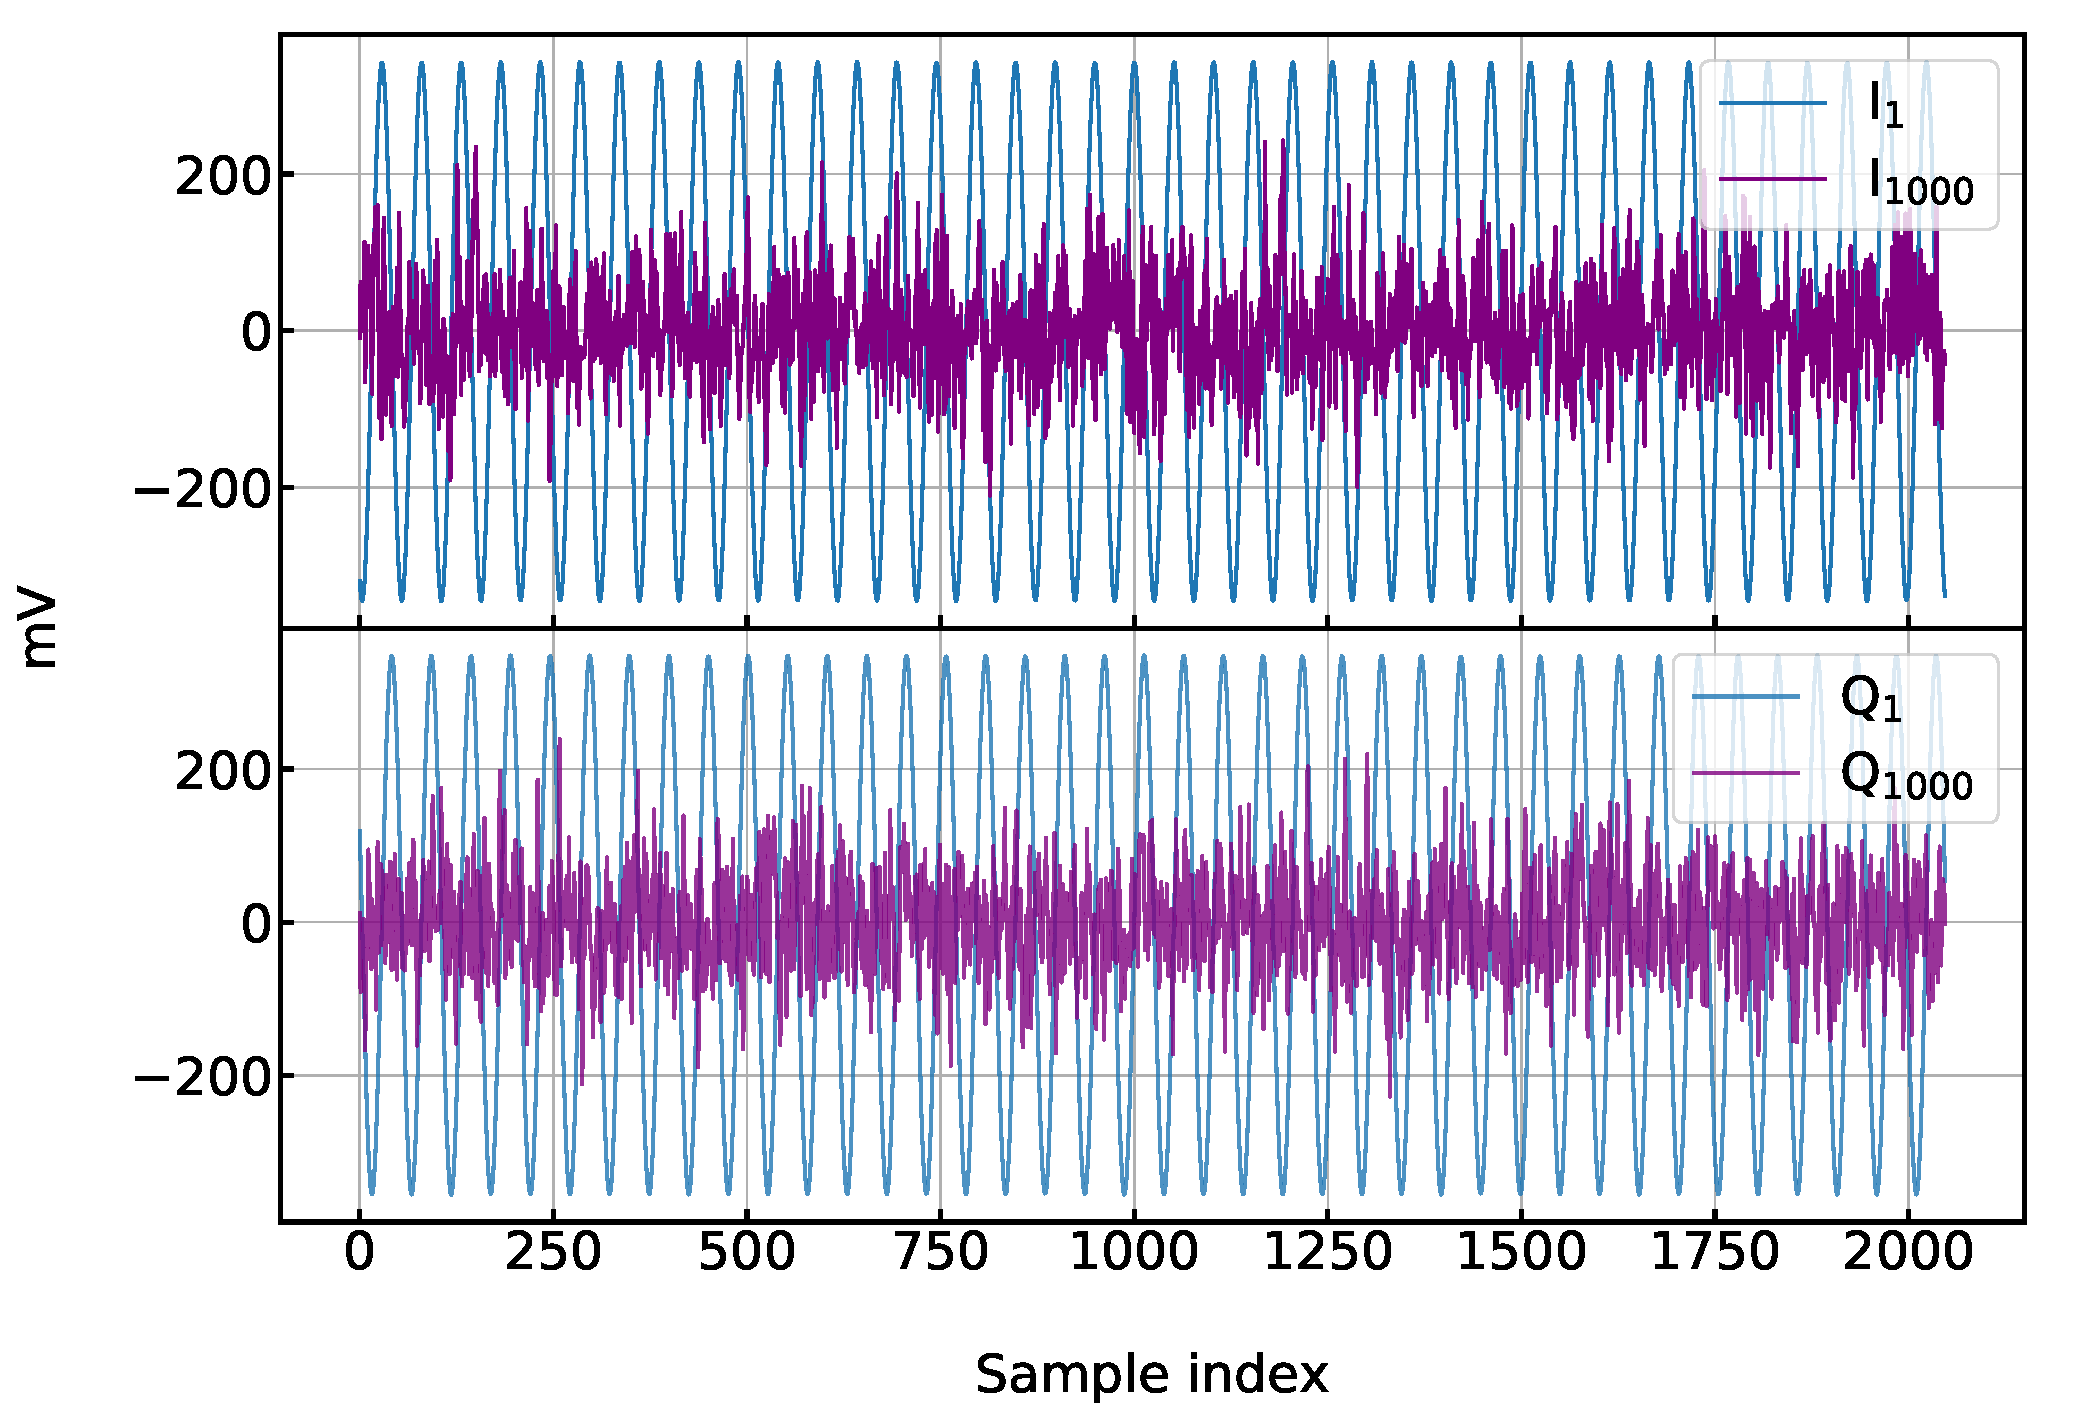
\includegraphics[width=\textwidth]{figures/readout/sim/adc}
\caption[~2,000 \macrocapwrap{$I/Q$} samples of a digitized waveform for a single tone at f = 50.0125~Hz, and 1000 evenly spaced tones.]{2,000 \macrocapwrap{$I/Q$} samples of a digitized waveform at \macrocapwrap{$f = 50.0125$}~Hz (blue), and for a tone comb consisting of 1000 evenly spaced tones.}
\label{fig:adc}
\end{figure}

\subsection{Coarse Channelization: The PFB-FFT}\label{pfb}

Inside the firmware, the digitized tone comb is processed using two consecutive stages of channelization. The first stage of channelization is a PFB-FFT (AKA filterbank). A detailed description of the PFB is found in \citet{price2016spectrometers}. Utilizing a PFB before an FFT allows for frequency response of the FFT bins to be shaped according to the chosen PFB parameters. Specifically, the PFB is intended to minimize the two most deleterious side-effects of FFTs, which are spectral leakage and scalloping loss.

A PFB accomplishes this by multiplying a segment of timestream (for either $I$ or $Q$) with a window function, dividing the windowed segment into $P$ `phases' of length $N_{FFT}$ (the poly-phases), and summing each of the $P$ phases. The summed segment of length $N_{FFT}$ is then fed into a FFT, also of length $N_{FFT}$ (the PFB-FFT is the combination of the two). The PFB acts as a set of sub-filters which condition the FFT bin transfer functions so that they are more rectangular than they would be otherwise. Lower side-lobe levels can be achieved by widening the the FFT bins.

The PFB-FFT is implemented using the CASPER \texttt{pfb\_fir} and \texttt{biplex\_fft} blocks. For the PFB, we use a $P = 4$ taps, a bin scaling factor of 2, and a Hamming window for the filter coefficients. The bin scaling factor of 2 widens the FFT bins so that they overlap at -6~dB. Their width at FWHM is 450~kHz. On each clock cycle, the biplex FFT receives two consecutive complex time ordered samples $I_{0}, I_{1}, Q_{0}, Q_{1}$, and outputs the complex amplitudes ($\widetilde{I}_{0}, \widetilde{I}_{1}, \widetilde{Q}_{0}, \widetilde{Q}_{1}$ of two consecutive ($k$, $k + 1$) frequency bins. One $N = 1024$ FFT is processed every 512 clock cycles, corresponding to an FFT-rate of 500~kHz. A synchronization pulse which is emitted on the last clock cycle before the first valid data of each consecutive FFT is used to synchronize all following stages of the firmware. Since the average individual detector bandwidth is $\sim$50~kHz, several detectors may safely fall within a single FFT bin. Each bin pair output by the FFT is concatenated into a single 72-bit word (4 $\times$ 18-bit) before being stored in block RAM (BRAM) in the FPGA for channel selection.

\begin{figure}[!htbp]
\centering
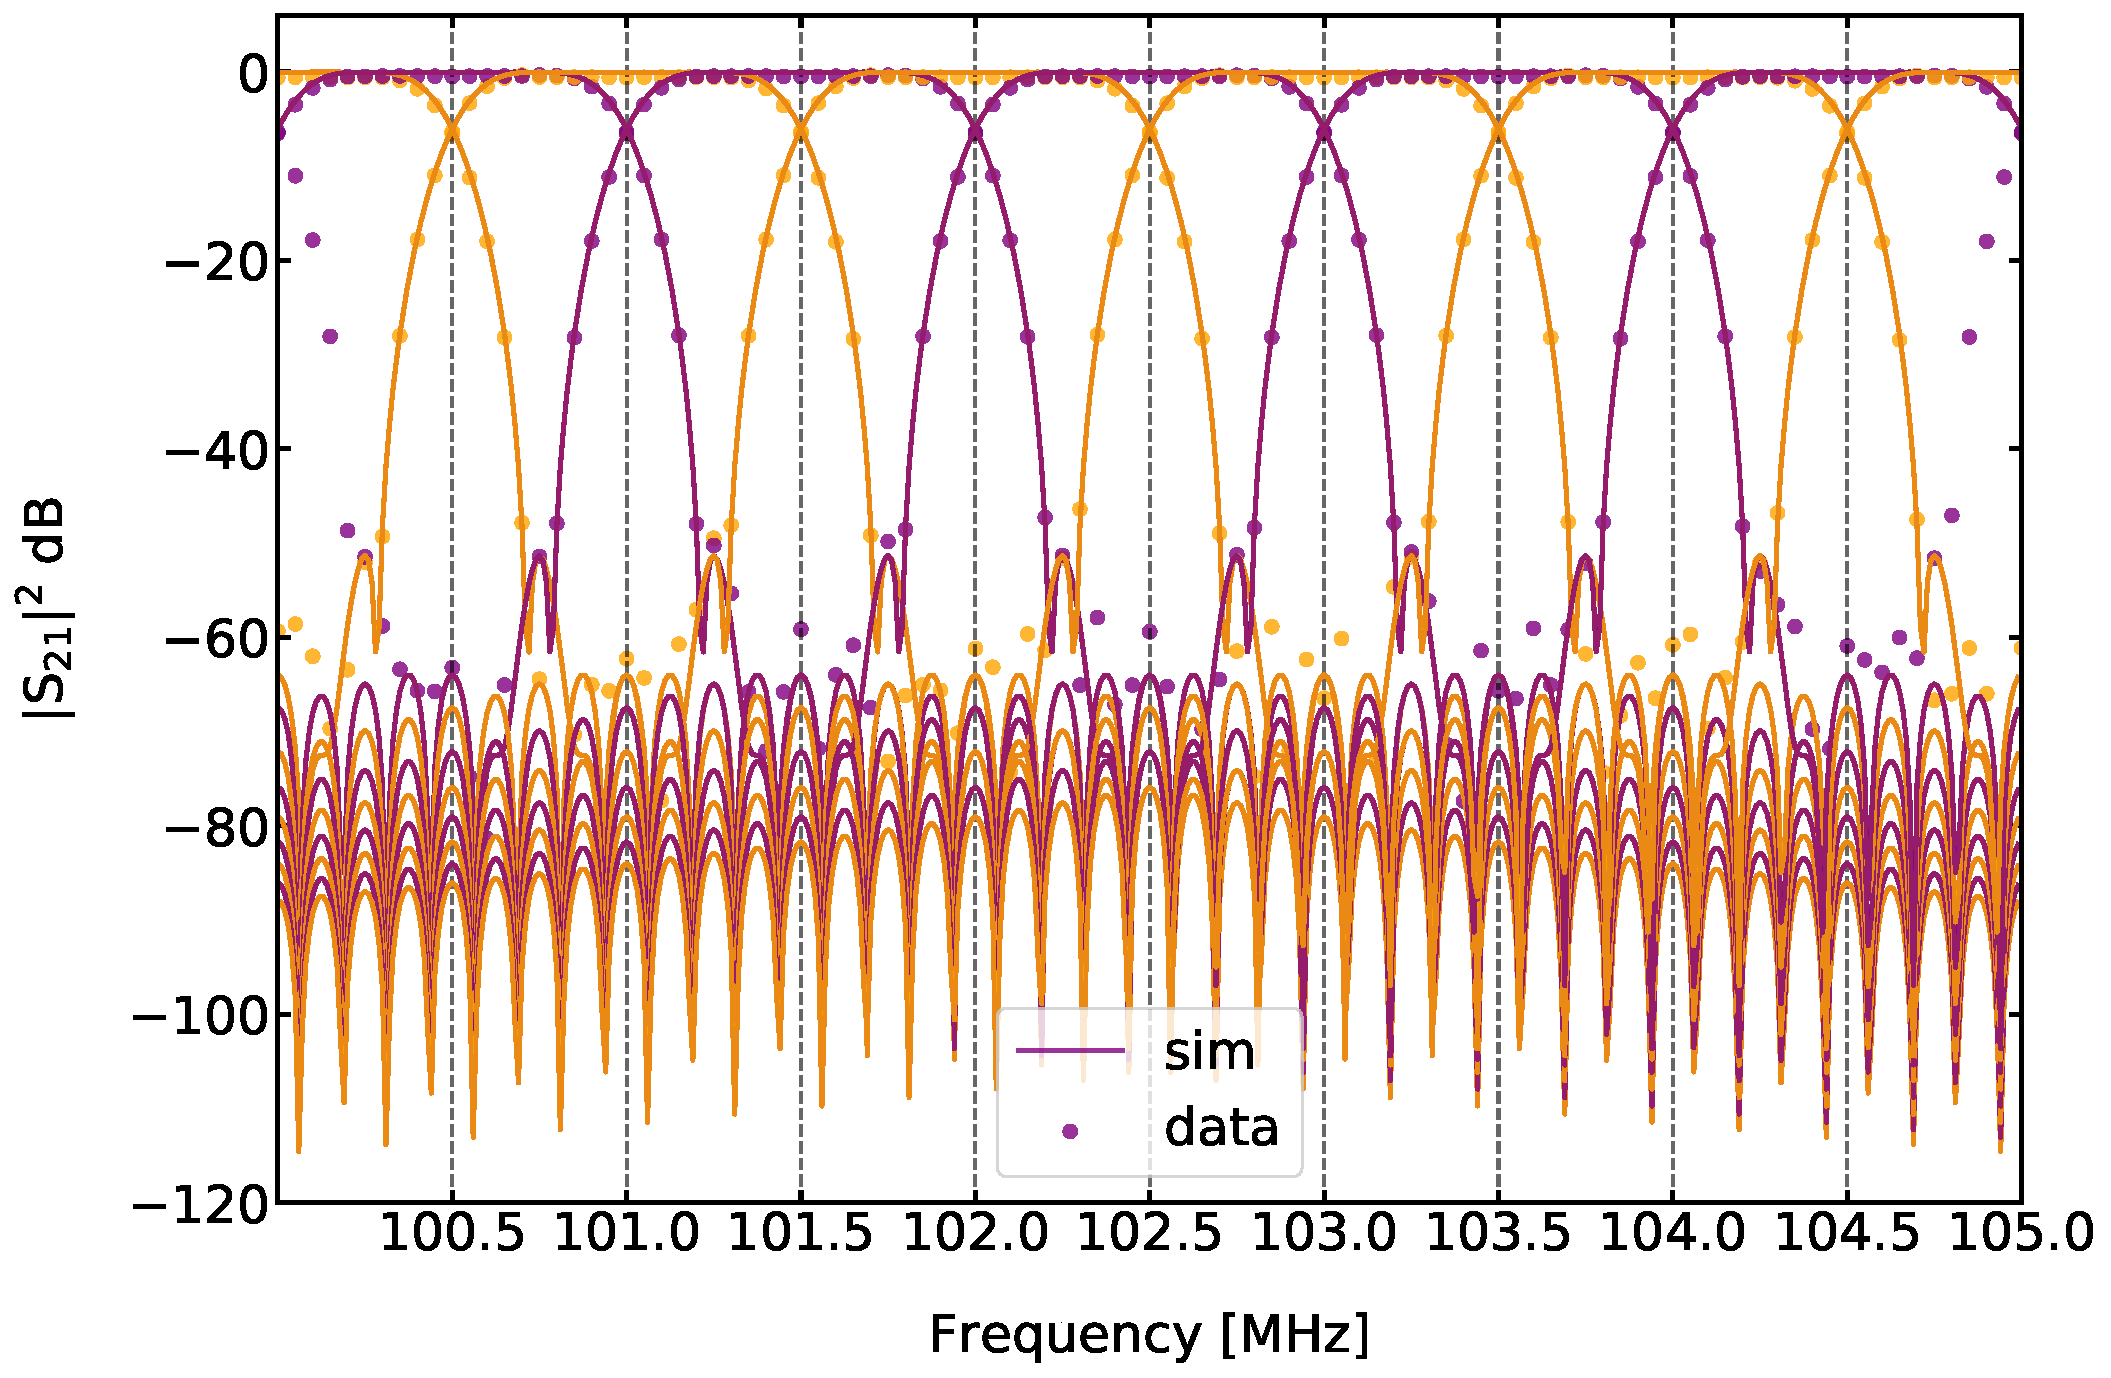
\includegraphics[width=\textwidth]{figures/readout/sim/pfb_fft_comp}
\caption[~A 5~MHz section of the transfer function of the firmware PFB-FFT, showing measured (dots) and simulated values (lines).]{A 5~MHz section of the transfer function of the firmware PFB-FFT, showing measured (dots) and simulated values (lines). The PFB has widened the FFT bins so that they overlap at -6~dB. Their FHWM width is 450~kHz.}
\label{fig:pfb fft zoom}
\end{figure}

\subsection{FFT Bin Selection}\label{bin select}

When the LEKID resonant frequencies are irregularly spaced (as is the case for the BLAST-TNG arrays), some PFB-FFT bins contain multiple probe tones, while others remain empty (containing only noise). Only the former set of bins requires further channelization. The channel selection logic requires that up to 1024 channels from the FFT bin stream be selected within 512 clock cycles. To manage this while continuously streaming data, a buffered switch is constructed using Xilinx dual-port BRAM blocks. During software synthesis of the $I/Q$ waveform buffers, a list of up to 1024 bins is pre-calculated based on known resonator frequencies and loaded into a dual-port `bin select' BRAM. The list may consist of any combination of the 1024 available bin indices, including a single bin index repeated 1024 times. If only a subset of bins is required, any unused RAM addresses are initialized to zero. Once the bin list is loaded into RAM, the bins are referred to as channels, with the channel order corresponding to the order of the original list. During operation, the bin indices for two consecutive channels are read out in parallel from the dual-port RAM. Each bin index is halved to represent the clock cycle (`clock address') corresponding to its offset in cycles from the zeroth FFT bin, and these clock addresses are to be used as read addresses for another dual-port RAM containing the bin data. In the data RAM, the contents of two consecutive bins are stored in each address slot.

In read mode, the contents of two bins are presented at each output port of the dual-port data RAM, the addresses of which are chosen by the clock addresses of the desired bin indices. Out of the four available bins to choose from on each cycle, only one member of each pair is desired. To determine which member of each bin pair to use, the least significant bit of the desired bin index is used to operate a switch that slices the proper bin from each pair. The new pair of bins is then passed through a MUX selector and sent to the first stage of the DDC. To facilitate continuous readout, the bin selector is duplicated into a read branch and a write branch, which together form a buffered switch.

The bins which are selected for further processing are hereafter referred to as channels.

\subsection{Fine Channelization: Digital Down Conversion}\label{ddc}

As was discussed in Section~\ref{tone comb} The PFB-FFT operates on the digitized ADC timestream once every 512 clock cycles, and therefore any probe tone waveforms that have a period longer than the filterbank length of 1024 samples will exhibit unwanted phase rotation over the course of several FFTs. This results in amplitude modulation of $\widetilde{I}$ and $\widetilde{Q}$, where the AM frequency $f_{k} - f_{pr}$. One approach to circumventing this issue would be to use a longer FFT, with bins so narrow that each $f_{pr}$ falls very near to a bin center. The MUSIC firmware employed this approach, with a $2^{16}$-point FFT, resulting in bin width of $\sim${7.5}~kHz (\citet{duan2010open}). However, this method relies on the LEKID frequency spacing being somewhat uniform. Instead, we use digital down conversion (DDC) to demodulate the residual AM. The technique, which was previously implemented in the ARCONS firmware \citep{mchugh2012readout}, has the advantage of using fewer FPGA resources then the long PFB-FFT approach.

To downconvert each channel, the $\widetilde{I}/\widetilde{Q}$ output timestreams from each FFT bin are multiplied with their corresponding $I_{DDC}$/$Q_{DDC}$ entries from the DDC LUT. With each clock cycle, two consecutive channels are operated on in parallel. A single cycle of the operation involves performing the calculation:

\begin{equation}
  (\widetilde{I} + j\widetilde{Q})(Q_{DDC} + jI_{DDC})
\end{equation}

where $\widetilde{I}/\widetilde{Q}$ are of data type 18.17, $I_{DDC}/Q_{DDC}$ are 16.15, and the resulting output $I/Q$ values are 19.17. During this process, FFT bins which contain multiple channels are downconverted once per channel. For successful down conversion to occur, each channel of the DDC LUT must be synchronized with its corresponding $\widetilde{I}/\widetilde{Q}$ timestream at the output of the FFT. Otherwies, on system start, the first channel arriving at the down converter will be out of sync channel-wise with its corresponding DDC tone by some number of clock cycles between 0 and 512. This `DDC shift' is constant for a given bitstream file, but due to differences in how the System Generator places the logic during each compilation, the DDC shift varies by a small number of clock cycles between different bitstreams.

For each firmware file, the DDC shift can be discovered on system startup by using an algorithm built into the readout sofware (see Section~\ref{software}). The software steps through each possible DDC shift using the variable delay block while monitoring the snap block data from the DDC for a single channel. At each shift, a software FFT of $\widetilde{I}/\widetilde{Q}$ is compared to that of $I_{DDC}/Q_{DDC}$. When the delay has been set properly, the FFTs will match. Once the shift is known, it is programmed into the variable delay block using a software register, and the value is thereafter left unchanged.

As stated above, FFT bins which contain $N$ probe tones are downconverted $N$ times. Each of the $N$ channels which result from this process contain the both the downconverted probe tone, centered at DC, as well as non-zero signal contributions from the other probe tones which were present in the FFT bin prior to downconversion. These adjacent tones must be filtered out. Two methods were explored in order to achieve this. The first method is to add a low-pass FIR filter after the DDC, which is narrow enough to filter out any adjacent tones. The second method, which is what is used in the BLAST-TNG firmware, is to accumulate the $I/Q$ values for each channel (see Section~\ref{accum}). Accumulation both filters out the adjacent tones (it is a boxcar filter), and reduces the sample rate.

Relative to downsampling by accumulation, the FIR has the disadvantage of requiring many FPGA resources (delays, adders and multipliers). Because the $I/Q$ samples at the output of the DDC are time-multiplexed (equivalently, channel-multiplexed) ($I_{\mathrm{chan0}}/Q_{\mathrm{chan0}}$, $I_{\mathrm{chan1}}/Q_{\mathrm{chan1}}$, ..., $I_{\mathrm{chanN}}/Q_{\mathrm{chanN}}$) the FIR must also act in a time-multiplexed fashion. At the output of the DDC, the samples of any given channel appear once every 512 clock cycles. Therefore, the FIR must include a matching latency of 512 clock cycles between every addition. Following \citet{strader2016digitial}, the $n$th $I$ value to appear at the output of the FIR is therefore:

\begin{equation}
  I_{\mathrm{out}}[n] = \sum _{m=0}^{M - 1} h[m]I_{\mathrm{in}}[n - 512m]
\end{equation}

where $m$ is the channel index and $h$ is a filter coefficient. The filter coefficients are calculated in software, using a hamming or hanning window, and then programmed into software registers by the user. During system operation they can be reprogrammed at any time.

The need for long latencies make it difficult for System Generator to meet the design's timing constraints during the placement and routing stage of firmware compilation. In addition, to narrow the signal bandwidth from 500~kHz to $\sim$1~kHz requires the use of many filter taps ($\mathcal{O}(100))$. By simply co-adding (accumulating) consecutive samples from each channel, both filtering and downsampling can be achieved simultaneously, with less resource utilization. Ultimately, this was the option that was taken for the BLAST-TNG firmware.

Figure~\ref{fig:ddc1} and~\ref{fig:ddc1000} show frequency domain examples of the downconversion process for one channel from a tone comb consisting of one and 1000 tones. In both figures, the top frame shows the input signal to the DDC, $X = \sqrt{\widetilde{I}^{2} + \widetilde{Q}^{2}}$, the middle frame shows the DDC tone $X_{DDC}$, and the bottom frame shows the downconverted output signal $Y$. The spurs which are visible at either side of the central tone are due to the effects of quantization errors in the software FFT. In the channel from the multitone comb shown in Figure~\ref{fig:ddc1000}, the group of spurs centered at -50~kHz relative to the main tone is due to sideband leakage in the IF modulator. The sideband tones are down $\sim$-20 dB relative to the main tone's peak, and are averaged out during the accumulation stage.

\begin{figure}[!htbp]
\centering
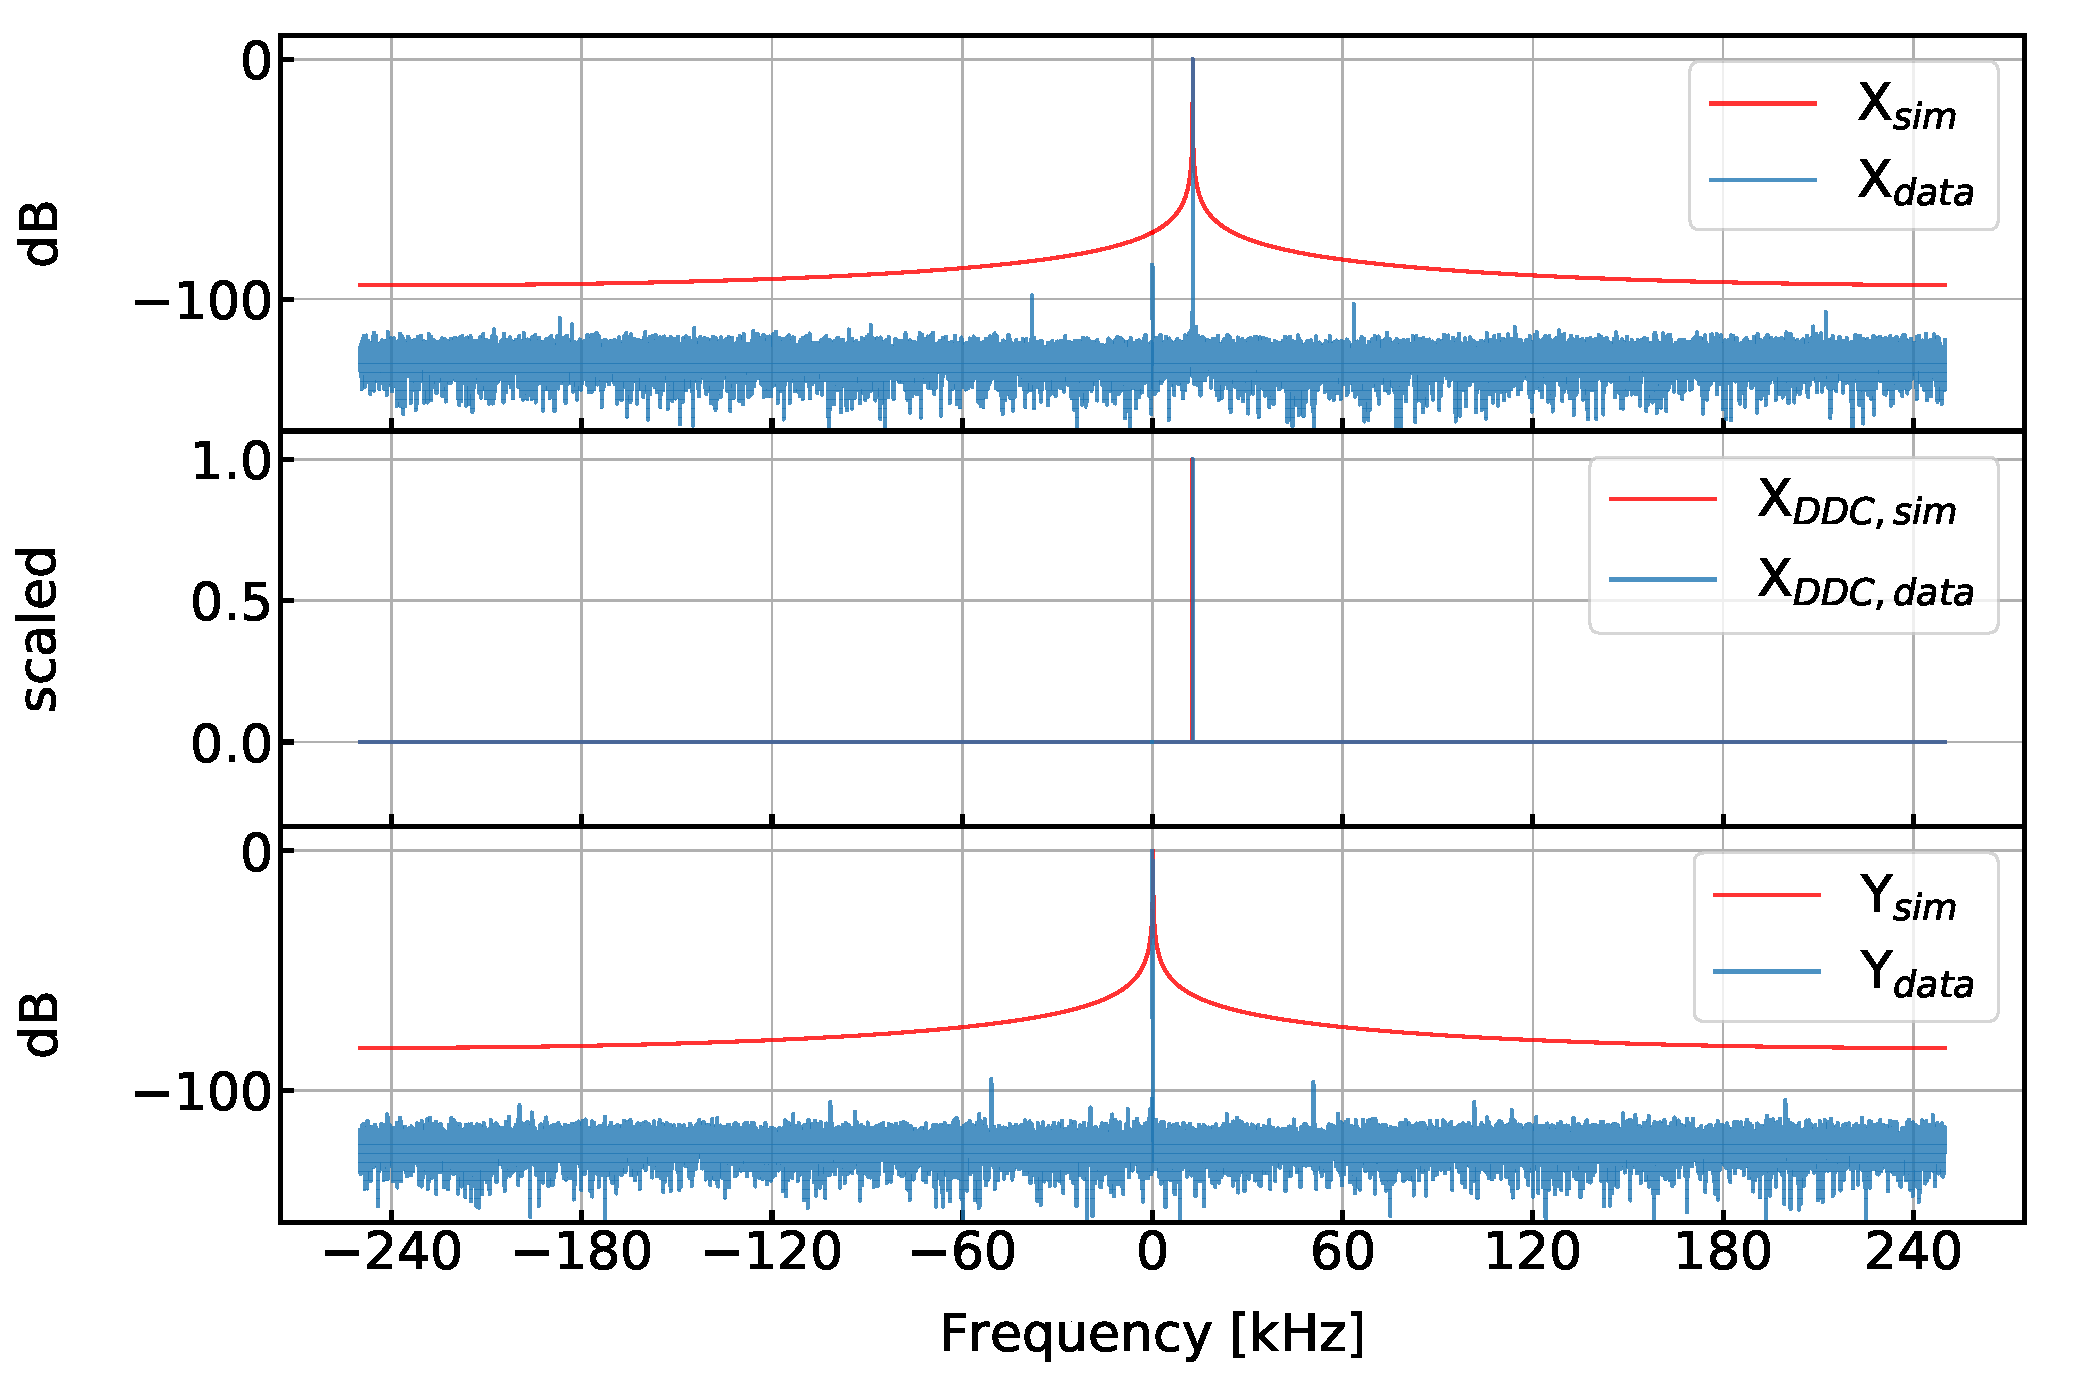
\includegraphics[width=\textwidth]{figures/readout/sim/ddc_sim_0}
\caption[~An example of the frequency domain DDC products (measured and simulated) for one channel of a tone comb consisting of a single tone.]{An example of the frequency domain DDC products (measured and simulated) for one channel of a tone comb consisting of a single tone.}
\label{fig:ddc1}
\end{figure}

\begin{figure}[!htbp]
\centering
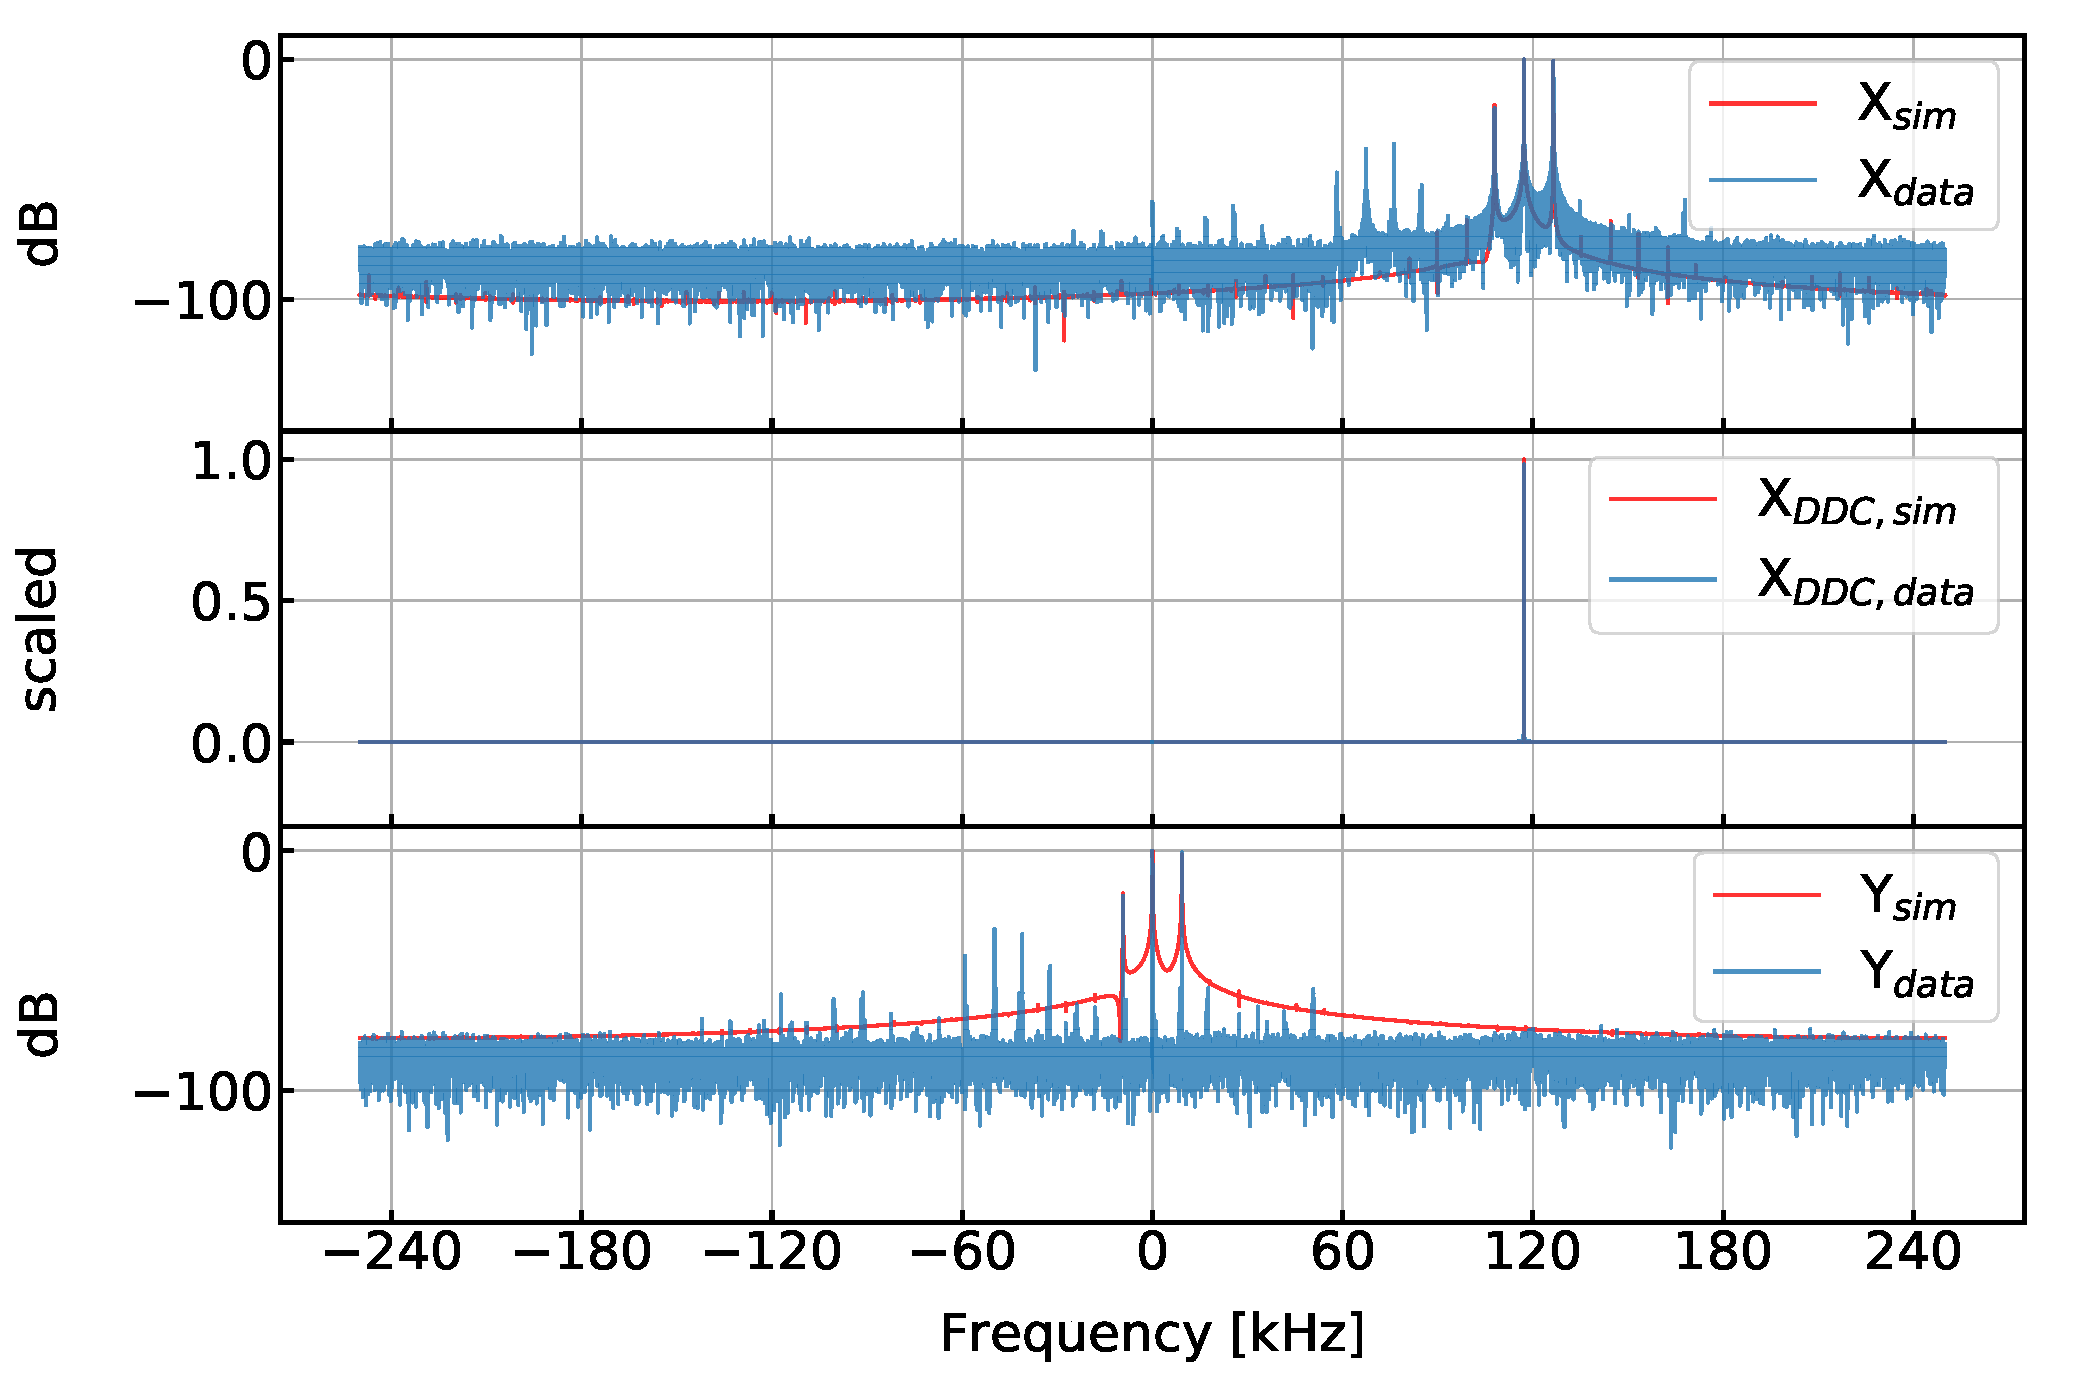
\includegraphics[width=\textwidth]{figures/readout/sim/ddc_sim_100}
\caption[~An example of the frequency domain DDC products (measured and simulated) for one channel of a tone comb consisting of 1000 tones.]{The frequency domain DDC products for one channel of a tone comb consisting of 1000 probe tones, with measured (blue) and simulated data (red).}
\label{fig:ddc1000}
\end{figure}

\begin{comment}
\begin{figure}[!htbp]
\centering
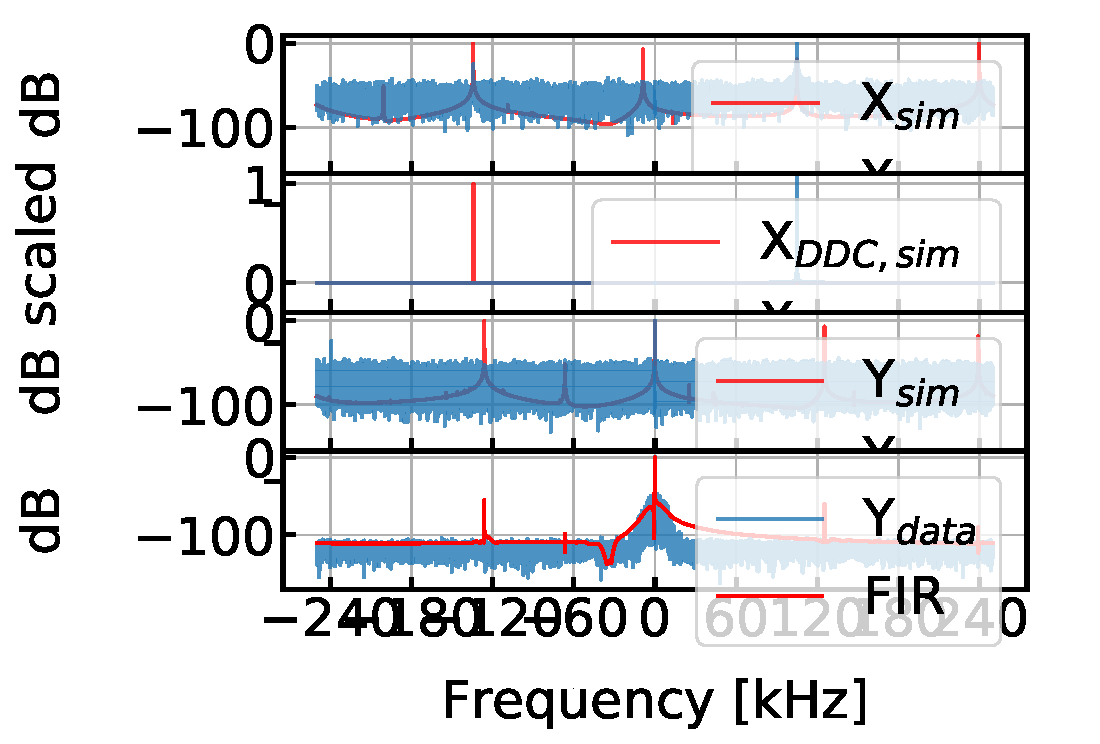
\includegraphics[width=\textwidth]{figures/readout/sim/ddc_sim_11}
\caption[~An example of the frequency domain DDC products (measured and simulated) for one channel of a tone comb consisting of 628 tones, with the FIR applied to the DDC output.]{The frequency domain DDC products for one channel of a tone comb consisting of 628 probe tones, with measured (blue) and simulated data (red). An FIR has been applied to the DDC output timestream.}
\label{fig:ddcFIR}
\end{figure}
\end{comment}

\subsection{Accumulation and Downsampling}\label{accum}

The downconverter outputs $I/Q$ samples at a rate of $f_{DDC} = 500$~kHz. The $I/Q$ timestreams at the output must be downsampled in order to output data at the desired rate. In the version of the firmware which does not contain the post-DDC FIR filter, the downconverted channels still contain signal from probe tones which were within the same PFB-FFT bin. While downsampling by decimation would require further filtering, downsampling by accumulation both decreases the data rate and filters out any signal which is non-periodic within the length of the accumulation.

Both downsampling and filteration are achieved by coherent channel-wise accumulation of the $I/Q$ values. The length of the accumulation is configured using a software register. The total number of accumulations used determines the bandwidth of the channels which are output by the system. For BLAST-TNG, the accumulation length is set to $2^{19}$ clock cycles, which corresponds to $N_{\mathrm{accum}} = 1024$. The resulting readout frequency $f_{ro} = 488.2815$~Hz, and the channel bandwidth $B_{\mathrm{chan}} = f_{ro}/2 = 244.14$~Hz. Because the number of accumulations can be adjusted by factors of 2, $f_{ro}$ may be set to values of $\approx$~30, 61, 122, 244, 488 or 976~Hz. The firmware architecture does not support $f_{ro} > 976$~Hz.

Accumulation is performed using CASPER vector accumulator blocks of length 512. During the additions, the $I/Q$ values are permitted to grow to 32-bits. The averaging function of the accumulator is effectively a box-car filter, which provides low-pass filtering of the channel timestreams. It is not necessary to complete the average with division by the total number of accumulations. Following accumulation, the channel values are sent to the packetization stage. Figure~\ref{fig:accum} shows the uncorrected transfer function (frequency response) for the 512~MHz readout band for a tone comb comprised of 1000 evenly spaced channels (the `VNA' comb). The orange trace was measured in digital loopback. In digital loopback, the DAC output is filtered and then input directly into the ADC. The blue trace show the full RF loopback (containing all IF electronics). The ripples in the RF loopback trace are a product of the frequency response from each IF component. This transfer function can be corrected for using software, by calculating and applying the inverse transfer function for each readout slice (see Section~\ref{TRF}).

\begin{figure}[!htbp]
\centering
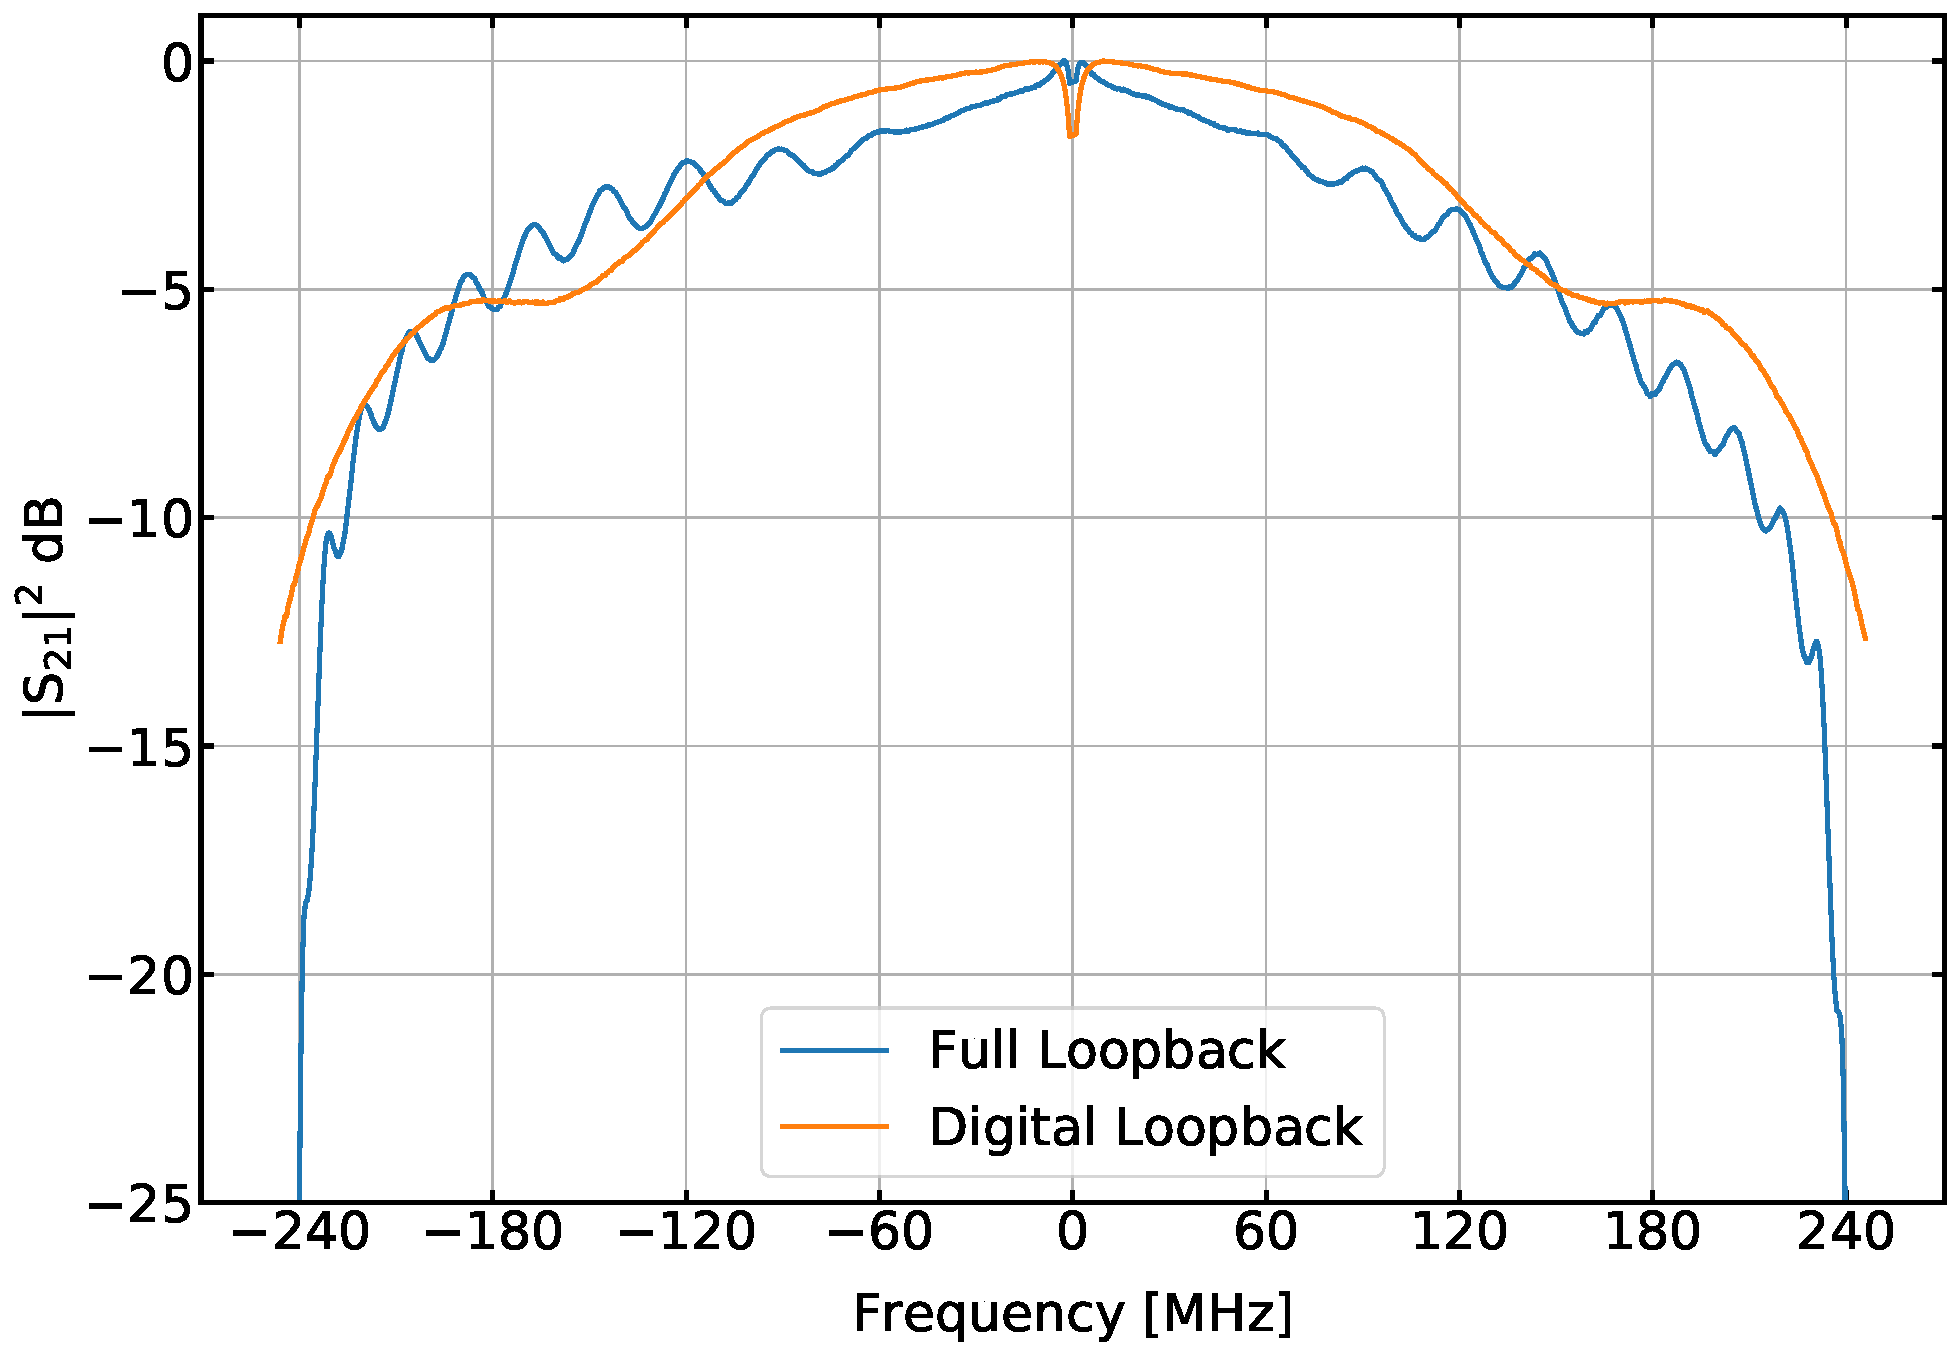
\includegraphics[width=\textwidth]{figures/readout/sim/accum_1000_lpf_nolpf}
\caption[~The transfer function of the accumulator (\macrocapwrap{|S$_{21}$|$^{2}$}), for a tone comb consisting of 1000 tones, in digital and RF loopback.]{The transfer function of the accumulator (|S$_{21}$|$^{2}$), for a tone comb consisting of 1000 tones, in digital and RF loopback.}
\label{fig:accum}
\end{figure}

\subsubsection{UDP Packetization and Time Stamping}\label{packets}

UDP packetization is performed using the CASPER 1GbE block. Because the block accepts only one byte at a time, each 4-B $I$ or $Q$ word must be sliced byte-wise before being input to the block.

The data packet size is fixed at 8234-B, regardless of the number of channels which is used. Figure~\ref{fig:data packet} shows the structure of a single UDP frame. Each packet contains a 42-B header, and 8192-B of data, which includes the $I/Q$ values for each channel, as well as time stamp and checksum information. The UDP header contains the source and destination MAC addresses, IP addresses and UDP ports, where the source values correspond to the FPGA Ethernet device on the ROACH2 board, and the destination values correspond to the data acquisition computer (DAQ). Each of these parameters is chosen by the user and programmed into the firmware using software registers during system startup.

After the header, there are 8192-B allocated for data storage. The first 8218-B contain the $I/Q$ values, which are stored as signed, 4-B words in little-endian:

\begin{itemize}[nosep]
  \item Words 1--512: $I$, channels 0--512
  \item Words 513--1024: $I$, channels 0--512
  \item Words 1025--1536: $I$, channels 513--1024
  \item Words 1537--2032: $I$, channels 513--1016
\end{itemize}

\vspace{5mm}

The last 8 $Q$ slots are used to store timestamp values, which limits the maximum channel count to 1016. The final 64-B of each packet contain timetamp information, a data checksum, and a free 4-B slot which can contain extra diagnostic information chosen by the user. The timing information is contained in 4 separate words, which are:

\begin{itemize}[nosep]
  \item ctime: The absolute Linux time, taken from the flight computer, and truncated to~$\upmu$s precision.
  \item PPS count: The number of elapsed PPS pulses since the PPS reset register was toggled.
  \item clock count: The number FPGA clock cycles which have elapsed between PPS counts.
  \item packet count: The number of packets which have been generated since the PPS reset register was toggled.
\end{itemize}

\vspace{5mm}

As described in Section~\ref{timing}, the combination of these values allows for the acquistion time of each data packet to be sychronized with the other telescope subsystems (most crucially, the pointing system) to within the required precision of $\sim$1~ms.

\begin{figure}[!htbp]
\centering
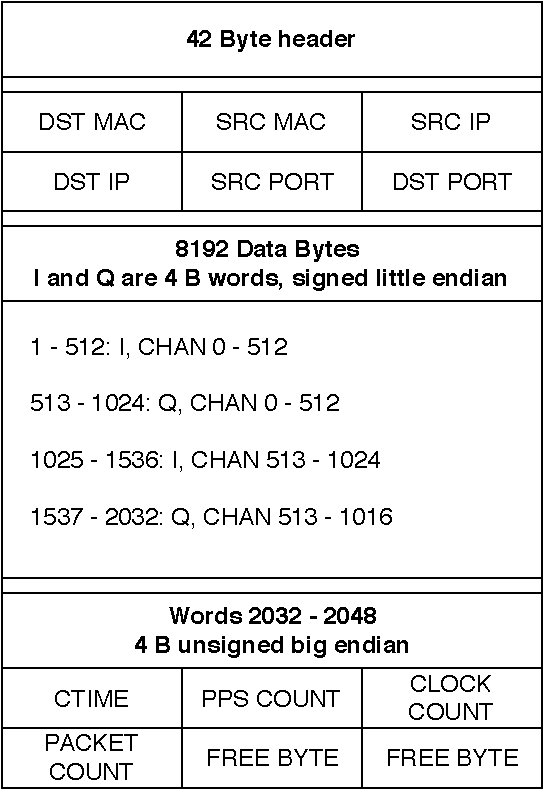
\includegraphics[scale=0.75]{figures/readout/roach_packet}
\caption[~ROACH2 UDP packet structure.]{The structure of a ROACH2 UDP packet}
\label{fig:data packet}
\end{figure}

\section{Noise Verification}\label{noise verify}

In this section, we describe the verification of the WN and FN system requirements described in Sections~\ref{white noise} and~\ref{flicker noise}. To characterize these noise properties, we use the one-sided PSD, $S_{xx}(f)$:

\begin{equation}\label{eq:psd}
  S_{xx}[f]={\frac {1}{N f_{s}}}\left|\sum _{n=1}^{N}x_{n}e^{-j2\pi f n/f_{s}}\right|^{2}
\end{equation}

To obtain a better estimate of the PSD than Equation~\ref{eq:psd} can provide, we use the Welch Periodogram (WP) \citep{welch1967use}. The WP is an asymptotically unbiased estimator of the PSD. In Welch's method, a timestream is divided into $K$ windowed segments of equal length. The periodogram is calculated for each segment, and then averaged. The segments may also be overlapped in time. The variance of the WP is reduced by a factor of $1/K$ relative to a regular periodogram, at the expense of lower frequency resolution. The WP can be written as:

\begin{equation}\label{eq:WP}
S_{xx}[f] = \frac{1}{K} \sum_{n=0}^{K - 1}\frac{1}{f_{s} M} \left| \sum_{n=0}^{N - 1} x_{n,w} e^{-j2\pi f n / f_{s} }\right|^{2}
\end{equation}

where $x_{n,w}$ is a windowed version of the time series, and $M$ is the length of each segment. To fit the noise PSDs, we use a modified version of Leeson's equation, which empirically models the phase noise spectrum produced by a resonator \citep{lesson1966simple}. The model is a three-parameter fit to \gls{Sphase}:

\begin{equation}\label{eq:PSD fit}
  S_{\phi,fit}(f) = W\left[ 1 + \gls{fc}/f + \left( \frac{B_{\mathrm{res}}}{f} \right)^{2} (1 + \gls{fc}/f) \right] \qquad \left[  \frac{\mathrm{rad}^{2}}{\mathrm{Hz}} \right]
\end{equation}

where $W$ is the WN level, the resonator bandwidth $B_{\mathrm{res}} = (f_{0}/2\gls{Qr})$, and \gls{fc} the FN corner-frequency. The PSDs are measured in digital and RF loopack. In digital loopback, the MUSIC board DAC $I/Q$ outputs are passed through anti-aliasing filters and then fed directly into the ADCs. RF loopback includes the IF electronics. To simulate the gain of the BLAST-TNG cryostat, a 20~dB attenuator is placed between the RF out and RF in ports of the readout slice.

Figure~\ref{fig:psd 1000 fit} shows an example fit (red) using Equation~\ref{eq:PSD fit} to the median PSD of a tone comb containing 1000 evenly spaced tones (blue), in digital loopback mode. In this particular example, the FN corner frequency $\gls{fc} \approx 0.5$~Hz, and the WN level is $\sim$-98~dBc/Hz.

\begin{figure}[!htbp]
\centering
\includegraphics[width=\textwidth]{figures/readout/sim/c1000_PSD_fit}
\caption[~A fit of a modified Leeson's equation to the median PSD for a tone comb containing 1000 evenly spaced tones.]{A fit (red) of a modified Leeson's equation to the median PSD (blue) for a tone comb containing 1000 evenly spaced tones.}
\label{fig:psd 1000 fit}
\end{figure}

In digital loopback mode, the noise was measured for tone combs containing 1, 100, 500, 618 and 1000 tones. In the tone combs containing 100, 500 and 1000 tones, the frequencies were evenly spaced by $\approx$~490~kHz. The tone comb with length 618 uses resonator frequencies which were identified for the 350~$\upmu$m array during detector testing at NASA's Columbia Scientific Balloon Facility in July, 2018 (618$_{350\mu m}$). These tones are not evenly spaced (see the discussion about detector yields in Chapter 4). The median PSDs calculated from each tone comb are shown in Figure~\ref{fig:dig loopback noise}. Table~\ref{tab:dig loopback} lists the WN level, in dBc/Hz and dB/Hz (converted using the method described in Section~\ref{white noise}, as well as the estimated CF (using Equation~\ref{eq:whitenoise}).

For the single tone comb, the WN level is measured to be $\approx$-143~dBc/Hz, which is within $\sim$1~dB of the theoretical minimum predicted by Equation~\ref{eq:whitenoise}. The WN levels for the evenly spaced tone combs are also close to their expected values. The 618$_{350\mu m}$ tone comb has a median WN level of $\approx$-105~dBc/Hz, which is close to the level measured for 1000 evenly spaced tones. This small amount of excess noise is attributed to the uneven spacing of the probe tones, which creates intermodulation products in the analog modulator/demodulators. For each tone comb, the FN corner frequency is $\approx$0.5~Hz.

\begin{table}[!htbp]
\centering
\begin{tabular}{@{}llll@{}}
  \dtoprule
  N tones & S$_{\phi}$ (dBc/Hz) & S$_{\delta f / f}$ (dB/Hz) & Crest Factor est. (dB) \\ \midrule
  1 & -143 & -244 & 3 \\
  100 & -113 & -215 & 11 \\
  500 & -108 & -209 & 10 \\
  618$_{350\mu m}$ & -105 & -206 & 12.5 \\
  1000 & -105 & -206 & 10 \\ \dbottomrule
  \\
\end{tabular}
\caption[~Digital loopback noise levels as a function of number of probe tones.]{The digital loopback WN levels as a function of 1, 100, 500, 618 and 1000 tones. \macrocapwrap{618$_{350\mu m}$} is the tone comb for the 350~\macrocapwrap{$\upmu$m} band tones used during the 2018 Palestine instrument integration for BLAST-TNG. \macrocapwrap{\gls{Sff}} is calculated according to Equation \macrocapwrap{\ref{eq:Sff est}}, with \macrocapwrap{\gls{Qr} = 2.85 $\times$ 10$^{4}$}. The PSDs shown are the median of the PSDs calculated for each \macrocapwrap{$N$} value, from 60~s timestreams. \macrocapwrap{$CF$} is the estimated crest factor, in dB.}
\label{tab:dig loopback}
\end{table}

\begin{figure}[!htbp]
\centering
\includegraphics[width=\textwidth]{figures/readout/sim/LB_noise}
\caption[~Digital loopback WN levels as a function of 1, 100, 500, 618 and 1000 tones.]{The digital loopback WN levels as a function of 1, 100, 500, 618 and 1000 tones. \macrocapwrap{618$_{350\mu m}$} is the tone comb for the 350~\macrocapwrap{$\upmu$m} band tones used during the 2018 Palestine instrument integration for BLAST-TNG. \macrocapwrap{\gls{Sff}} is calculated according to Equation \macrocapwrap{\ref{eq:Sff est}}, with \macrocapwrap{\gls{Qr} = 2.85 $\times$ 10$^{4}$}. The PSDs shown are the median of the PSDs calculated for each \macrocapwrap{$N$} value, from 60~s timestreams.}
\label{fig:dig loopback noise}
\end{figure}

The same median-PSD analysis was performed in RF loopback, using tone combs containing a single tone, the 618$_{350\mu m}$ tones and an evenly spaced comb of 1000 tones (25 of which were removed from the data due to unusually high noise). The results of the analysis are shown in Figure~\ref{fig:rf loopback noise}. Table~\ref{tab:rf loopback} lists the WN levels as in Table~\ref{tab:dig loopback}, except the third column shows the estimated IF noise, in dB. The IF noise was estimated using Equation~\ref{eq:whitenoise} with the CF values in Table~\ref{tab:dig loopback}, and is found to be $\sim$5~dB in each measurement.

The WN level of the single tone is measured as -136~dBc/Hz, and those of the 1000 and 618$_{350\mu m}$ combs are $\sim$~-98 dBc/Hz. These values are safely below the WN system requirement derived in Section~\ref{white noise}. However, the margin of error is only a few dB. As in digital loopback mode, the FN corner frequencies are $\approx$~0.5~Hz. While this value also satisfies the system requirement, there is little margin for error. It is therefore important to keep the noise contribution of the IF electronics as low as possible.

\begin{figure}[!htbp]
\centering
\includegraphics[width=\textwidth]{figures/readout/sim/IF_LB_noise}
\caption[~The RF loopback WN levels as a function of 1, 618 and 975 tones.]{The RF loopback WN levels as a function of 1, 618 and 975 tones. 618$_{350\mu m}$ is the tone comb for the 350~$\upmu$m band tones used during the 2018 Palestine instrument integration for BLAST-TNG. \gls{Sff} is calculated according to Equation~\ref{eq:Sff est}, with\gls{Qr} = 2.85 $\times$ 10$^{4}$. The PSDs shown are the median of the PSDs calculated for each $N$ value, from 60~s timestreams.}
\label{fig:rf loopback noise}
\end{figure}

The WN and FN noise estimates presented in this section are in close agreement with those presented in \citet{gordon2016}, which have been measured using similar firmware and IF electronics.

\begin{table}[!htbp]
\centering
\begin{tabular}{@{}llll@{}}
\dtoprule
N tones & S$_{\phi}$ (dBc/Hz) & S$_{\delta f / f}$ (dB/Hz) & IF Noise (dB) \\ \midrule
1 & -136 & -237 & 4 \\
618$_{350\mu m}$ & -98 & -199 & 5 \\
1000 & -98 & -199 & 5.5 \\ \dbottomrule
\\
\end{tabular}
\caption[~RF loopback noise levels for different numbers of probe tones.]{The RF loopback WN levels as a function of 1, 618 and 975 tones. 618$_{350\mu m}$ is the tone comb for the 350~$\upmu$m band tones used during the 2018 Palestine instrument integration for BLAST-TNG. \gls{Sff} is calculated according to Equation \ref{eq:Sff est}, with \gls{Qr} = 2.85 $\times$ 10$^{4}$. The PSDs shown are the median of the PSDs calculated for each $N$ value, from 60~s timestreams. The last column is the estimated IF noise, in dB.}
\label{tab:rf loopback}
\end{table}

\begin{comment}
\begin{figure}[!htbp]
\centering
\includegraphics[width=\textwidth]{figures/readout/sim/350_phase_PSDs}
\caption{The white noise in RF loopback mode as a function of probe tone frequency.}
\label{fig:350um PSD comp}
\end{figure}
\end{comment}

\section{Readout Software}\label{software}

A custom software interface is required to operate the ROACH2 firmware and IF electronics, both in a lab setting and during instrument operation. The extent to which the software is automated depends on the context in which the system is being used. For example, if the system is to be used on a balloon platform (e.g, BLAST-TNG, OLIMPO), most if not all of the software functionality should be automated. At a ground/mountain-based observatory (e.g, TolTEC, MUSCAT, SuperSpec), user input on the observer's part should be incorporated when the outcome of a decision can affect the quality of the data (e.g., during the channel selection stage of operation). Basic housekeeping functions, which include uploading the FPGA firmware, initializing software registers such as the DDC delay and writing and programming probe tone combs tones frequency combs, should be automated no matter the context. Other functions, such as the acquisition of diagnostic snap-block data and the setting of RF power levels via the programmable attentuators, should be easily accessible to the operator.

For lab-based system operation, an open-source \texttt{Python}-based software was developed, known as kidPy (\url{https://github.com/sbg2133/kidPy}). KidPy is a terminal user interface (TUI) which enables the manual operation of every step which is required to run the readout and acquire data. For the BLAST-TNG flight code (MCP), kidPY was ported to \texttt{C} and fully automated. The BLAST-TNG readout software and in-flight operational strategy is detailed in Chapter~\ref{mcp}.

\chapter{Instrumental Characterization of BLAST-TNG}\label{blast_data}

The following sections describe the characterization of the instrumental performance of BLAST-TNG in the lead-up to the 2018/2019 launch attempt from NASA's Long Duration Balloon site (LDB) in Antarctica. Because the camera contains over 2,500 polarization sensitive pixels distributed over three wavebands, it would not be feasible to describe the individual performance of each pixel within this document. Instead, we present a detailed data reduction for a single pixel, which is then extended to statistical results which summarize the overall performance of each BLAST-TNG band. The instrumental performance is characterized by numerous parameters, many of which are interdependent and can not be directly measured. Instead, they must be inferred from the results of empirical measurements, which in some cases can be checked against a model, such as the one presented in Chapter~\ref{kid_model}.

Out of all of the instrumental parameters that could be examined, a small number of them directly determine how well the camera will perform in terms of its mapping speed and on-sky sensitivity to sub-mm intensity and polarization. These parameters are the detector yields and NEP or NET (sensitivity), optical efficiency, passband shapes and polarization efficiencies. The in-flight performance is also directly related to the operation of the detector readout. For example, to utilize the full dynamic range of each detector during flight will require that the readout probe tones be periodically retuned in frequency and amplitude. Notes on readout operation are interspersed with the following description of how each of the aforementioned parameters has been estimated.

The chapter is organized as follows:

\begin{itemize}[nosep]
  \item Section~\ref{sweeps} introduces detector frequency sweeps, frequency-domain channel identification, and detector yields.
  \item Section~\ref{timestreams} introduces the raw $I/Q$ timestreams which are generated by the readout, and how they are calibrated into frequency units which are proportional to absorbed optical power.
  \item Section~\ref{responsivities} discusses the responsivities to absorbed optical power and changes in base temperature.
  \item Section~\ref{sensitivity} presents sensitivity estimates for each band (NEP) and describes how these estimates are made using a combination of sweeps, timestreams and optical tests.
  \item In Section~\ref{applying model} we compare the measured data for a single channel from the 350~$\upmu$m and 250W arrays to results from the parametric LEKID model presented in Chapter~\ref{kid_model}.
  \item In Section~\ref{histograms} we present histograms showing the distribution of important detector parameters for each of the five BLAST-TNG detector arrays.
  \item Section~\ref{optical tests} presents the data reduction and results of passband mapping (Section~\ref{fts}) and polarization efficiency (Section~\ref{pol eff}).
\end{itemize}

The data used in the following analysis was mostly acquired in May, 2018 (Philadelphia, PA), July, 2018 (NASA's Columbia Scientific Ballooning Facility (CSBF) Palestine, Texas), and winter 2018/2019 (NASA Long Duration Balloon facility (LDB), Antarctica).

\section{Detector Sweeps}\label{sweeps}

The BLAST-TNG detectors are distributed between five LEKID arrays, with one for the 350 and 500~$\upmu$m bands, and three for the 250~$\upmu$m. The three 250~$\upmu$m arrays (hereafter referred to as the 250U, 250V and 250W) reside on the same chip, but are read out independently. The 250V RF-chain malfunctioned during the pre-flight instrument integration at LDB, and we therefore do not present results for this channel from the Antarctic (`ice') campaign.

Every test of the detectors begins with a frequency sweep of the full 512~MHz RF-bandwidth occupied by each detector array. If the resonator frequencies are not known ahead of time, or have drifted by more than $\sim$1 resonator linewidth, the wide sweep is used to identify the channel frequencies (see Section~\ref{KID-finding}). A wide sweep (sometimes referred to as a `VNA' sweep) is performed by sweeping the 1,000 tone evenly-spaced search-comb over the 500~kHz gap between tones. The multitone comb is swept by stepping the local oscillator (LO) from one end of the 500~kHz gap to the other in frequency steps of $\approx$ 1~kHz. At each step, $I/Q$ data is saved to disk and co-added, with the number of data points taken at each frequency typically being $\sim$20. The wide-sweeps take $\sim$30 seconds to complete. Plotted as a function of RF-frequency, the data shows $\gls{S21}V_{\mathrm{in}}$ of the detector readout chain (hereafter simply referred to as \gls{S21}), where $V_{\mathrm{in}}$ is the amplitude of the probe-tone comb at the output of the ROACH2 digital-to-analog converters (DACs).

\subsection{The Wide-sweep Frequency Response}\label{freq response}

Figures~\ref{fig:350 wide sweep} and Figures~\ref{fig:350 zoom} show an overlay of two example sweeps of the 350~$\upmu$m array. The blue sweep was taken in May, 2018, and the orange trace was taken in July, 2018. The blue sweep shows the raw (uncorrected) frequency response of the readout system and detector chain, whereas the orange trace was produced by applying several corrections to the readout probe tone amplitudes. The transfer function correction is described in Section~\ref{TRF}. Both sweeps were taken with the cryostat window exposed to the $\sim$300~K thermal radiation of the highbay. A (2.85\%) 4\% neutral-density filter (NDF) inside the receiver's cold-optics limits the optical power which reaches the detectors (after accounting for an optical efficiency \gls{opt_eff} of $\sim$30, and a detector efficiency \gls{det_eff} of $\sim$80\%) to $\sim$10~pW.

The frequency response (or transfer function) of the system contains information about the frequency response of every element in the detector chain. The primary contributors are the ROACH2 electronics, input and output side intermediate-frequency (IF) electronics, room-temperature as well as cryogenic cabling, the cryogenic low-noise amplifier (LNA) and the detector arrays themselves. In the frequency domain, the total system response is the product of the transfer function for each of the individual elements.

The envelope of the uncorrected \gls{S21} sweep contains several notable features:

\begin{itemize}[nosep]
  \item A gradual roll-off in power toward the band-edges.
  \item A steep roll-off in power at the band-edges.
  \item A deep null in the center of the band.
  \item A standing wave (ringing) pattern with a frequency of $\sim$30~MHz.
\end{itemize}

\begin{figure}[!htbp]
\centering
\includegraphics[width=\textwidth]{figures/blast_data/sweeps/350_wide_sweep}
\caption[~Comparison between raw and corrected wide-sweeps of the \macrocapwrap{350~$\upmu$m} array.]{Uncorrected (blue) and corrected (orange) ROACH2 wide-sweeps of the BLAST-TNG 350~$\upmu$m array.}
\label{fig:350 wide sweep}
\end{figure}

\begin{figure}[!htbp]
\centering
\includegraphics[width=\textwidth]{figures/blast_data/sweeps/350_wide_sweep_zoom}
\caption[~A zoomed-in region of an unprocessed and processed wide-sweep of the \macrocapwrap{350~$\upmu$m} array.]{A zoomed-in region of an unprocessed (blue) and processed (orange) wide-sweep of the 350~$\upmu$m array.}
\label{fig:350 zoom}
\end{figure}

The gradual roll-off in power toward the band-edges can be attributed to the MUSIC board's DAC frequency response, the LNA frequency response at low frequency ($\sim$500~MHz) as well as to the frequency response of modulator and demodulator (the demodulator contains 300~MHz low-pass filters). The steeper roll-off that begins at $\sim$15~MHz from the lower and upper band-edges is from the baseband anti-aliasing filters. The ringing pattern in the \gls{S21} envelope is due to a combination of the anti-aliasing filters and warm and cold cabling. The null in the center of the band is where the LO frequency is located. Typically, no probe tones are generated inside a 20~MHz band centered at the LO frequency.

The remaining features in the \gls{S21} trace shown in Figure~\ref{fig:350 wide sweep} are the individual resonator transfer functions. The 350~$\upmu$m array contains $\sim$750 resonators (within the readout band-- see Section~\ref{yields}). A small number of resonators with their horn antennas blocked off, known as $\textit{darks}$, have noticeably deeper resonances than the other detectors. The distribution of resonator dip-depths varies widely across the band. This spread is due to variations in several parameters, including intrinsic resonator quality factors, readout powers and optical loading. Much of the large scale variations in readout power can be corrected for by applying a global inverse transfer function to the probe comb. In addition to this, the tone power for each channel may be individually adjusted. The process of determining and applying the inverse transfer function correction is described in the following section.

\subsection{Transfer function Correction}\label{TRF}

As discussed in Section~\ref{freq response}, the uncorrected \gls{S21} frequency response revealed by the ROACH2 wide sweeps contain large scale features that may contribute to uneven detector performance across the band. Some of these features can be compensated for by applying an inverse transfer function to the amplitudes of the DAC probe comb. The goal of applying this correction is to correct for, as much as possible, any transfer function contributions from the input side of the detector chain (relative to the cryostat). All output side transfer functions (after and including the detectors) are left untouched. The components whose transfer functions will be corrected include the ROACH2 output-side electronics (both digital and analog) and any coaxial cables between the ROACH2 electronics and the detector arrays.

The output side system transfer function is measured by connecting the RF output of the ROACH2 IF electronics to a spectrum analyzer. The spectrum is then saved to disk, and interpolated in frequency as needed. Examples of the intermediate products used in the transfer function calculation are shown in Figure~\ref{fig:350 TRF}. The blue trace is the raw output of the RF modulator. A $\sim$10~dB roll-off is present between the center of the band and either band-edge. In addition to correcting for the envelope of the ROACH2 comb, a power ramp (shown as a green line) is added to the correction to compensate for frequency dependent loss in the cryostat cables. The inverse transfer function which is then applied to the DAC comb amplitudes is shown in orange.

The frequency-dependent cable loss which occurs inside the cryostat is visible in Figures~\ref{fig:VNA comp 350} to~\ref{fig:VNA comp 500}, which show \gls{S21} sweeps taken with a VNA (purple) compared to corrected ROACH2 \gls{S21} sweeps (orange) for each BLAST-TNG array. The cable loss is $\sim$10 dB across the readout-band. With the application of the inverse transfer function, much of the roll-off in the envelope of the frequency response is compensated for. For each array, a slightly different slope for the power ramp is used. An illustration of the effect of using different slope corrections for the 350~$\upmu$m array is shown in Figure~\ref{fig:trf slopes}, for slopes of 5, 8 and 10~dB (across the entire readout band).

\begin{figure}[!htbp]
\centering
\includegraphics[width=\textwidth]{figures/blast_data/sweeps/r3_transfunc}
\caption[~Intermediate products used in the transfer function calculation for the \macrocapwrap{350~$\upmu$m} array.]{Intermediate products used in the transfer function calculation for the 350~$\upmu$m array.}
\label{fig:350 TRF}
\end{figure}

\begin{figure}[!htbp]
\centering
\includegraphics[width=\textwidth]{figures/blast_data/sweeps/350_VNA_overplot}
\caption[~A \macrocapwrap{350~$\upmu$m} ROACH2 sweep from the Palestine integration, with a VNA sweep from May, 2018.]{A 350~$\upmu$m ROACH2 sweep (orange) from the Palestine integration, with a VNA sweep from May, 2018 (purple).}
\label{fig:VNA comp 350}
\end{figure}

\begin{figure}[!htbp]
\centering
\includegraphics[width=\textwidth]{figures/blast_data/sweeps/250W_VNA_overplot}
\caption[~A 250W ROACH2 sweep from the Palestine integration, with a VNA sweep from May, 2018.]{A 250W ROACH2 sweep (orange) from the Palestine integration, with a VNA sweep from May, 2018 (purple).}
\label{fig:VNA comp 250W}
\end{figure}

\begin{figure}[!htbp]
\centering
\includegraphics[width=\textwidth]{figures/blast_data/sweeps/250U_VNA_overplot}
\caption[~A 250U ROACH2 sweep from the Palestine integration, with a VNA sweep from May, 2018.]{A 250U ROACH2 sweep (orange) from the Palestine integration, with a VNA sweep from May, 2018 (purple).}
\label{fig:VNA comp 250U}
\end{figure}

\begin{figure}[!htbp]
\centering
\includegraphics[width=\textwidth]{figures/blast_data/sweeps/250V_VNA_overplot}
\caption[~A 250V ROACH2 sweep from the Palestine integration, with a VNA sweep from May, 2018.]{A 250V ROACH2 sweep (orange) from the Palestine integration, with a VNA sweep from May, 2018 (purple).}
\label{fig:VNA comp 250V}
\end{figure}

\begin{figure}[!htbp]
\centering
\includegraphics[width=\textwidth]{figures/blast_data/sweeps/500_VNA_overplot}
\caption[~A 500~\macrocapwrap{$\upmu$m} ROACH2 sweep from the Palestine integration, with a VNA sweep from May, 2018.]{A 500~$\upmu$m ROACH2 sweep (orange) from the Palestine integration, with a VNA sweep from May, 2018 (purple).}
\label{fig:VNA comp 500}
\end{figure}

\begin{figure}[!htbp]
\centering
\includegraphics[width=\textwidth]{figures/blast_data/sweeps/trf_slopes}
\caption[~350~\macrocapwrap{$\upmu$m} output transfer function corrections with slopes of 5, 8 and 10~dB.]{350~$\upmu$m output transfer function corrections with 5, 8 and 10~dB slopes accounting for frequency dependent cable loss in the croystat. A VNA trace is shown for comparison.}
\label{fig:trf slopes}
\end{figure}

%%%%%%%%%%%%%%%%%%%%%%%%%%%%%%%%%%%%%%%%%%%%%%%%%%%%%%%%%%%%%%%%%%%%%%%%%%%%%%%
% FIND KIDS
%%%%%%%%%%%%%%%%%%%%%%%%%%%%%%%%%%%%%%%%%%%%%%%%%%%%%%%%%%%%%%%%%%%%%%%%%%%%%%
\subsection{Channel Identification}\label{KID-finding}

The channel frequencies for each array can be determined from a wide ROACH2 sweep (or VNA trace of \gls{S21}). For BLAST-TNG, the steps of the KID-finding algorithm are:

\begin{enumerate}[nosep]
  \item Despike the \gls{S21} trace in linear-space.
  \item Apply a high-pass filter (HPF) to flatten the trace.
  \item Put the trace into log-space, and apply a second HPF\@.
  \item Apply a low-pass filter (LPF) to remove any remaining spurs.
  \item Identify all points in trace below the dip-depth threshold.
  \item Step through points and enforce frequency spacing condition.
  \item Eliminate frequencies in masked regions.
  \item Calculate channel amplitudes from interpolated output TRF\@.
  \item Save channel frequencies and amplitudes to disk.
\end{enumerate}

\vspace{5mm}

\begin{figure}[!htbp]
\centering
\includegraphics[width=\textwidth]{figures/blast_data/sweeps/350FK_HPF_PAL}
\caption[~The channel alignment and HPF step of the KID-finding algorithm.]{The channel alignment and HPF step of the KID-finding algorithm. The LPF (red) is subtracted from the \gls{S21} trace (blue) prior to frequency identification.}
\label{fig:350FK_HPF}
\end{figure}

This sequence is intended to be performed either at the start of a science observation, or when environmental conditions (fridge temperature drift, optical loading) have shifted the resonators far off of resonance. If the frequency shifts are less than $\sim$2 resonator linewidths, a target sweep may be used to recalibrate the readout frequencies in fewer steps (see Section~\ref{target sweeps}).

The preflight parameters used in the KID-finding process for each BLAST-TNG detector array are listed in Table~\ref{table:KID finding params}. The \gls{S21} sweep is high-pass filtered in (2) and (3) to flatten out the trace envelope as much as possible before identifying points below the dip-depth threshold. The high-pass filtering in (2) is achieved by subtracting a LPF from the data in linear-space. An example of this is shown in Figure~\ref{fig:350FK_HPF}, for the 350~$\upmu$m array. The close spacing of the channels makes it challenging to flatten out the inter-channel frequency space below a level of $\sim$0.1--0.5~dB. Consequently, a small number of `false' channels ($\sim$1--2\% of the total number) are identified by the KID-finding algorithm. The false channels can be manually flagged for removal, or added to the masked regions in (7). The dip-depth threshhold for the 500~$\upmu$m array is set to -0.5 dB due to the intrinsically low \gls{Qr} of the resonators. For the other arrays, the threshold is set to -1 dB.

During channel identification, a frequency spacing threshold of 80--100~kHz is enforced. If two channels are spaced by less than this threshold, the channel with the shallow dip-depth is omitted from the final frequency list. The masked regions listed in Table~\ref{table:KID finding params} are ignored during the KID-finding process. These regions include a 10~MHz window above and below the center of the band (f$_\mathrm{LO}$), and narrow bands which sometimes contain spurious noise thought to be associated with RF interference (RFI).

\subsection{Detector Yields}\label{yields}

\begin{table}[!hbtp]
  \centering
  \begin{threeparttable}
    \caption{Parameters used in KID-finding process for each BLAST-TNG detector array.}
\begin{tabular}{@{}llllll@{}}
\dtoprule{}
 & 250U~$\upmu$m & 250V~$\upmu$m & 250W~$\upmu$m & 350~$\upmu$m & 500~$\upmu$m \\ \midrule
LPF f$_{c}$ (MHz) & 10 & 5 & 5 & 10 & 10 \\
Dip-depth thresh. (dB) & -1 & -1 & -1 & -1 & -0.5 \\
Spacing thresh. (kHz) & 100 & 100 & 100 & 100 & 100 \\
f$_\mathrm{LO}$ (MHz)\tnote{1} & 827 & 829 & 828 & 850 & 540 \\
f$_{\mathrm{low-cut}}$ (MHz) & 590 & 590 & 590 & 604.5 & 326 \\
f$_{\mathrm{high-cut}}$ (MHz) & 1060 & 1060 & 1060 & 1089 & 762 \\
f$_{\mathrm{mask,low}}$ (MHz)\tnote{2} &  & 820 & 751, 818 & 845 & 450.8, 535 \\
f$_{\mathrm{mask,high}}$ (MHz)\tnote{3} &  & 835 & 770, 838 & 855 & 451.8, 545 \\ \dbottomrule{}
\\
\end{tabular}
\begin{tablenotes}
\item [1] The LO center-frequency.
\item [2] The start frequencies of masked regions.
\item [3] The stop frequencies of masked regions.
\vspace{2mm}
\end{tablenotes}
\label{table:KID finding params}
\end{threeparttable}
\end{table}

Detector yields for each BLAST-TNG array determined using the ROACH2 readout during the Palestine and Antarctica integrations are listed in Table~\ref{table:det yields}. In the table, N$_{\mathrm{design}}$ refers to the number of channels on each array which were reported by NIST\@. With the exception of the 350~$\upmu$m array, this value is not necessarily the actual number of channels within the 512~MHz ROACH2 readout bandwidth. As a baseline channel count, we adopt the number of channels which were found by applying the KID-finding algorithm to dark VNA \gls{S21} sweeps taken during May, 2018 (N$_{\mathrm{May18,VNA}}$). The yields are then calculated by comparing the channel counts found during the Palestine and Antarctica integrations to N$_{\mathrm{May18,VNA}}$. The Palestine yields (Y$_{\mathrm{PAL/VNA}}$) are around 85\% for each array. During the Palestine integration, a $\sim$4\% neutral-density filter (NDF) was installed in the array. The NDF was not present during the Antarctica integration, and the increased optical loading on the arrays made it challenging to identify all of the channels (particularly in the case of the 500~$\upmu$m array). The 250V array was not used during ice testing due to a damaged component in the cold RF-chain.

\begin{table}[!htbp]
  \centering
  \begin{threeparttable}
    \caption[~Detector yields for each BLAST-TNG detector array.]{Detector yields for each BLAST-TNG detector array.}
\begin{tabular}{@{}llllll@{}}
\dtoprule{}
                        & 250U       & 250V \tnote{1} & 250W    &350~$\upmu$m       & 500~$\upmu$m \\ \midrule
N$_{\mathrm{design}}$\tnote{3}   & 612        & 612         & 612        & 775\tnote{2}     & 468     \\
N$_{\mathrm{May18,VNA}}$\tnote{4}& 500        & 521         & 495        & 683              & 381     \\
N$_{\mathrm{PAL}}$ \tnote{5}     & 390        & 237         & 412        & 626              & 326     \\
N$_{\mathrm{ICE}}$ \tnote{6}     & 508        &             & 466        & 619              & 260     \\
Y$_{\mathrm{VNA/design}}$\tnote{7} & 0.82     & 0.85        & 0.81       & 0.88             & 0.81    \\
Y$_{\mathrm{PAL/VNA}}$           & 0.78       & 0.45        & 0.83       & 0.92             & 0.86    \\
Y$_{\mathrm{ICE/VNA}}$           & 1.01       &             & 0.94       & 0.91             & 0.68    \\ \dbottomrule{}
\\
\end{tabular}
\begin{tablenotes}
\item [1] The 250V cold RF chain was damaged on the ice, and the array was not used during testing.
\item [2] Number of detectors within the readout band of 512 MHz.
\item [3] Number of detectors on each array, reported by NIST\@.
\item [4] Number of detectors identified in a May, 2018 VNA sweep.
\item [5] Number of detectors identified in ROACH sweeps during Palestine integration.
\item [6] Number of detectors identified in ROACH sweeps during preflight ice integration.
\vspace{2mm}
\end{tablenotes}
\label{table:det yields}
\end{threeparttable}
\end{table}

Figures~\ref{fig:350 VNA FK} to~\ref{fig:500 VNA FK} show the results of the KID-finding algorithm applied to the VNA, Palestine and Antarctica sweeps of each array. Selected channels are marked with red stars. The dip-depth threshold is shown as a dashed red line, and masked regions are highlighted in green.

% VNA overplot
\begin{figure}[!p]
\centering
\caption[~\macrocapwrap{350~$\upmu$m} array KID-finding results.]{350~$\upmu$m array KID-finding results for a VNA sweep (top) and ROACH2 sweeps from Palestine (middle) and the ice (bottom).}
\includegraphics[width=0.68\textwidth]{figures/blast_data/sweeps/350_May2018VNA_FK}
\includegraphics[width=0.68\textwidth]{figures/blast_data/sweeps/350_PAL_FK}
\includegraphics[width=0.68\textwidth]{figures/blast_data/sweeps/350_ICE_FK}
\label{fig:350 VNA FK}
\end{figure}

% 250 W

\begin{figure}[!p]
\centering
\caption[~250W array KID-finding results.]{250W array KID-finding results for a VNA sweep (top) and ROACH2 sweeps from Palestine (middle) and the ice (bottom).}
\includegraphics[width=0.68\textwidth]{figures/blast_data/sweeps/250W_May2018VNA_FK}
\includegraphics[width=0.68\textwidth]{figures/blast_data/sweeps/250W_PAL_FK}
\includegraphics[width=0.68\textwidth]{figures/blast_data/sweeps/250W_ICE_FK}
\label{fig:250W FK}
\end{figure}

% 250 U

\begin{figure}[!p]
\centering
\caption[~250U array KID-finding results.]{250U array KID-finding results for a VNA sweep (top) and ROACH2 sweeps from Palestine (middle) and the ice (bottom).}
\includegraphics[width=0.68\textwidth]{figures/blast_data/sweeps/250U_May2018VNA_FK}
\includegraphics[width=0.68\textwidth]{figures/blast_data/sweeps/250U_PAL_FK}
\includegraphics[width=0.68\textwidth]{figures/blast_data/sweeps/250U_ICE_FK}
\label{fig:250U FK}
\end{figure}

% 250 V

\begin{figure}[!p]
\centering
\caption[~250V array KID-finding results.]{250V array KID-finding results for a VNA sweep (top) and a ROACH2 sweep from Palestine (bottom).}
\includegraphics[width=0.68\textwidth]{figures/blast_data/sweeps/250V_May2018VNA_FK}
\includegraphics[width=0.68\textwidth]{figures/blast_data/sweeps/250V_PAL_FK}
\label{fig:250V FK}
\end{figure}

% 500
\begin{figure}[!p]
\centering
\caption[~\macrocapwrap{500~$\upmu$m} array KID-finding results.]{500~$\upmu$m array KID-finding results for a VNA sweep (top) and ROACH2 sweeps from Palestine (middle) and the ice (bottom).}
\includegraphics[width=0.68\textwidth]{figures/blast_data/sweeps/500_May2018VNA_FK}
\includegraphics[width=0.68\textwidth]{figures/blast_data/sweeps/500_PAL_FK}
\includegraphics[width=0.68\textwidth]{figures/blast_data/sweeps/500_ICE_FK}
\label{fig:500 VNA FK}
\end{figure}

\subsection{Target Sweeps}\label{target sweeps}

Once the channel frequencies for a given detector array have been identified, shorter frequency sweeps, hereafter referred to as target sweeps, may be performed in place of the wide-sweeps. Only tones which correspond to the frequency locations of resonators are used in the target sweep. The tones in the target frequency comb are referred to as channels. The initial channel amplitudes are chosen by interpolating the channel frequency onto the inverse transfer function template calculated for each array (see Section~\ref{TRF}). During instrument operation, target sweeps are done on regular intervals to calibrate the absolute frequency response of each channel. The frequency span of the sweep can be varied in the readout software, but is typically between $\sim$100--250~kHz, depending on the quality factor of the resonators.

An example of a 350~$\upmu$m target sweep, taken at CSBF, is shown in Figure~\ref{fig:350 targ fts}. Each channel is labeled with a number (the channel index) which ranges from 0 (to the right of the LO) to $N$ (to the left of the LO), where $N$ is the number of channels identified in the KID-finding stage. Figure~\ref{fig:350 targ ice} shows an overlay of two target sweeps taken during the LDB integration. The purple sweep was taken with the shutter closed, and the orange with the shutter open. Several parameters which are used to calculate the absolute frequency shift of each resonator can be extracted from the target sweeps. This calculation is described in Section~\ref{df calc}.

\begin{figure}[!htbp]
\centering
\includegraphics[width=\textwidth]{figures/blast_data/sweeps/350_targ_fts}
\caption[~An example \macrocapwrap{350~$\upmu$m} target sweep.]{An example 350~$\upmu$m target sweep.}
\label{fig:350 targ fts}
\end{figure}

\begin{figure}[!htbp]
\centering
\includegraphics[width=\textwidth]{figures/blast_data/sweeps/350_targ_ice_overplot}
\caption[~\macrocapwrap{350~$\upmu$m} target sweeps from the ice, with shutter open and closed.]{350~$\upmu$m target sweeps from the ice, with shutter open (orange) and closed {purple}.}
\label{fig:350 targ ice}
\end{figure}

\subsection{Readout Power Optimization}\label{readout power}

The readout probe tones have an effect on resonator frequencies and quality factors. These effects, and their relation to the nonlinear kinetic inductance, are discussed in Chapter~\ref{kid_model}. Figures~\ref{fig:may out atten} and~\ref{fig:may out atten bifurc} show the effects of varying the readout power for two different resonators on one of the 250~$\upmu$m arrays. In this example, the readout power was increased in six increments of 3~dB by decreasing the output attenuation in the ROACH2 IF electronics, producing a range of $\sim$ -90 to -72 dBm. The output attenuator settings, in dB, are listed in the figure legends.

The data shown in Figures~\ref{fig:may out atten} and~\ref{fig:may out atten bifurc} are overlays of target sweeps taken at each readout power. In each figure, the top panel shows $\left| \gls{S21} \right|^{2}$, the middle panel shows the phase of \gls{S21}, \gls{phiIQ}, and the bottom panel shows the $I/Q$ circle in the complex plane, in scaled raw units. It can be seen in both figures that above a certain readout power, the resonator frequency detuning and Q degradation becomes nonlinear (due to the nonlinear kinetic inductance). For both channels, the resonator detuning reaches $\sim$1 linewidth before the nonlinearity sets in. For the resonator in Figure~\ref{fig:may out atten bifurc}, bifurcation sets in before the last 6~dB of tone power stepping. The bifurcation is visible as a sharp discontinuity in each panel.

At lower readout powers, the effects seen in $\left| \gls{S21} \right|^{2}$, \gls{phiIQ} and in the $I/Q$ circle are similar to what would be observed from either optical or thermal loading. As tone power increases, the slope of the phase decreases, and the $I/Q$ circles become more elliptical.

In practice, the optical responsivity of each resonator is maximized at a slightly different readout power. As a rule of thumb, the optimal tone power can be set for each channel by first identifying that channel's bifurcation power, and then backing it off by $\sim$6~dB. The tone powers can also be optimized in a global sense, by adjusting the ROACH2 output attenuator while measuring the frequency noise on and off-resonance ($f_{0} + \sim$100~kHz). The on-resonance noise level is the sum of the LNA, detector and photon noise, whereas the off-resonance noise level reflects the LNA noise. Therefore, if the noise level on-resonance is greater than the off-resonance noise for a given channel, then the channel is assumed to be at least detector-noise limited. Above some attenuator setting, the vast majority of resonators should be biased in the detector-noise limited regime.

\begin{figure}[!ptbh]
\centering
\caption[~Sweeps at different tone powers for a single resonator.]{$\left| \gls{S21} \right|^{2}$, \gls{phiIQ} and $I/Q$ loops for target sweeps of a single 250~$\upmu$m channel over a range of readout powers.}
\includegraphics[width=0.68\textwidth]{figures/blast_data/sweeps/mag_tone_power_may}
\includegraphics[width=0.68\textwidth]{figures/blast_data/sweeps/phase_tone_power_may}
\includegraphics[width=0.68\textwidth]{figures/blast_data/sweeps/IQ_tone_power_may}
\label{fig:may out atten}
\end{figure}

\begin{figure}[!ptbh]
\centering
\caption[~Sweeps at different tone powers for a single resonator, showing bifurcation.]{$\left| \gls{S21} \right|^{2}$, \gls{phiIQ} and $I/Q$ loops for a range of tone powers, showing bifurcation.}
\includegraphics[width=0.68\textwidth]{figures/blast_data/sweeps/mag_tone_power_bifurc}
\includegraphics[width=0.68\textwidth]{figures/blast_data/sweeps/phase_tone_power_bifurc}
\includegraphics[width=0.68\textwidth]{figures/blast_data/sweeps/IQ_tone_power_bifurc}
\label{fig:may out atten bifurc}
\end{figure}

\section{Detector Timestreams}\label{timestreams}

The readout outputs two 32-bit samples, $I[n]$ and $Q[n]$, for each channel at a rate of 488.28125~Hz (once every $\approx$~2~ms). $I$ and $Q$ represent the demodulated channel amplitude: $\gls{S21}[n] = I[n] +jQ[n] $. With knowledge of the readout processing gain, it would be possible to convert $I$ and $Q$ into absolute units of volts. However, because it is \gls{phiIQ} which is proportional to the absorbed optical power, it is not necessary to perform this calibration. $I$ and $Q$ are therefore saved to disk in raw units, and then used to calculate the frequency shift of the resonator for each sample, \gls{df} (which is proportional to the phase shift of the probe tone). This process is described in the following section.

\subsection{Converting \macrocapwrap{$I/Q$} to \macrocapwrap{\gls{df}}}\label{df calc}

In the following, we describe the steps of the data reduction which are taken to convert the $I/Q$ timestreams to units of frequency shift, \gls{df}, relative to the resonant frequency of each channel. If the frequency responsivity is known, the system NEP can be calculated by measuring the frequency noise $(e_{f}/f_{0})^{2} = \gls{Sxx} = \gls{Sff}$ $[\mathrm{Hz}^{-1}]$ (see Section~\ref{sensitivity}).

To convert $I/Q$ to units of frequency requires either a recent target (or wide) sweep of the resonator. Hereafter, this sweep is referred to as the reference sweep. Two methods of converting \gls{S21} to frequency units are commonly used. These are the $I/Q$ gradient (\gls{gradIQ}) and the phase-fitting method. The relative advantages of each method are described in detail in \citet{barry2014development}. Choosing between the two methods entails a trade-off between computational efficiency and accurate representation of the frequency shift. The gradient method is more computationally efficient than the phase method at the expense of not accounting for the change in the shape of the resonant circle when $f_{0}$ is shifted far from resonance (more below). Ultimately, the gradient method underestimates the frequency noise by a factor of $\sim$1.5 \citep{barry2014development}.

For real-time estimates of \gls{df} during a measurement, we find that the $I/Q$ gradient method is preferred over the phase-fitting method. The gradient method is described in detail in \citet{d2013nika} (for a description of the phase method, see \citet{gao2008physics}). Here, we summarize its key elements. Using the reference frequency sweep, \gls{df} (in the continuous time domain) is calculated from \gls{S21} as:

% df
\begin{equation}\label{eq:df1}
   \delta f(t) = \frac{\delta \gls{S21}}{\nabla_{f}\gls{S21}} = \frac{\delta I(t) + j\delta Q(t)}{\nabla_{I,Q}}
\end{equation}

Rationalizing Equation~\ref{eq:df1} yields:

\begin{equation}\label{eq:df2}
    \delta f(t) = \frac{\delta I(t) \cdot dI/df + \delta Q(t) \cdot dQ/df}{(df/dQ)^{2} + (dQ/df)^{2}} - j\frac{\delta I(t) \cdot dQ/df - \delta Q(t) \cdot dI/df}{(df/dQ)^{2} + (dQ/df)^{2}}
\end{equation}

where all of the $I/Q$ values are with respect to the resonant frequency, $\delta I(t) = I(t) - I_{\mathrm{ref}}$ and $I_{\mathrm{ref}}$ ($Q_{\mathrm{ref}}$) are the $I/Q$ values on resonance at the time at which the reference sweep was taken. The \gls{df} values produced by this method are valid only if the resonator has shifted by less than a linewidth (see below). Figure~\ref{fig:IQ grad} shows an example \gls{gradIQ} calculation for one channel (channel 448) of the 350~$\upmu$m array. The value of \gls{gradIQ} which is used in Equations~\ref{eq:df1} and~\ref{eq:df2} is taken where $\left| \gls{gradIQ} \right|$ at its maximum. This point is marked with the dotted black line in Figure~\ref{fig:IQ grad}.

In practice, SNR variations in the target sweeps translate into errors in the \gls{gradIQ} calculation. During a measurement, it is possible to calibrate \gls{gradIQ} by chopping the LO in frequency by a fixed amount both above and below the center frequency. If the probe tone is perfectly centered on the resonant frequency, and \gls{Qr} is moderately high, the \gls{df} step observed in the timestreams for each channel should equal the chop \gls{df}. If the probe tone is within a resonator linewidth of $f_{0}$, but off-center relative to $f_{0}$, the \gls{df} observed in the timestreams will be asymmetric. If the probe tone is too far out of range of $f_{0}$, the LO chop will have little to no observable effect in the channel timestreams.

If the probe tone is known to be on or very near resonance, the LO chop provides a good indicator of the accuracy of the \gls{gradIQ} values. During the BLAST-TNG flight the LO chop will performed during each azimuth turnaround (the data acquired during these turnaround will not be used to make science maps). The \gls{df} chops which are imprinted into each channel's timestream can be used to calibrate the $I/Q$ data post-flight.

Figure~\ref{fig:lo chops} shows an example LO chop for one channel from the 250U, 350 and 500~$\upmu$m arrays, taken during pre-flight preparations at LDB\@. The frequency step-size is 2.5~kHz for the 250 and 350~$\upmu$m arrays, and 10~kHz for the 500~$\upmu$m. At the time when these LO chops were recorded, the probe tones were very close to $f_{0}$, and the channel \gls{df} values match the LO chop. The spikes in the data located around the frequency jumps are due to drop-outs in the LO signal when the synthesizer is stepped.

% LO chops ICE
\begin{figure}[!htbp]
\centering
\includegraphics[width=\textwidth]{figures/blast_data/timestreams/ice_lo_chops}
\caption[~LO chops for the 250U, 350 and 500~\macrocapwrap{$\upmu$m} arrays.]{LO chops for the 250U, 350 and 500~$\upmu$m arrays.}
\label{fig:lo chops}
\end{figure}

\subsection{Phase and Dissipation Quadratures}

In Equation~\ref{eq:df2}, the real part of \gls{df}, $\Re(\gls{df})$, represents the total frequency fluctuation in the phase quadrature (tangent to the $I/Q$ circle in the complex-plane), and the imaginary part of \gls{df}, $\Im(\gls{df})$, represents the fluctuation in the dissipation quadrature (orthogonal to the $I/Q$ circle). The noise in the dissipation quadrature is primarily from the LNA (($e_{f,\mathrm{diss}}/f_{0})^{2} = \gls{Syy}$). The noise in the phase quadrature which is not due to the amplifiers can be estimated as $\gls{Sxx} - \gls{Syy}$. If the detectors are photon noise limited, then $S_{\mathrm{phot}} \simeq \gls{Sxx} - \gls{Syy}$. In the photon noise limited regime, \gls{Sxx} should be greater than \gls{Syy}.

Figure~\ref{fig:timestreams} shows a 10~s timestream for channel 448 of the 350~$\upmu$m array, recorded at CSBF\@. The timestream is shown as $I$ (top, raw units), $Q$ (second from top, raw units), $\Re(\gls{df})$ (second from bottom, Hz) and $\Im(\gls{df})$ (bottom, Hz). Figure~\ref{fig:example chan} shows $\left| \gls{S21} \right|^{2}$ (top), \gls{phiIQ} (middle) and the $I/Q$ circle for the example channel. The dashed red line in $\left| \gls{S21} \right|^{2}$ is a fit to the data which has been used to estimate the resonator parameters listed in Table~\ref{table:350 example chan}. The estimated parameters are: $f_{0}$, dip-depth, \gls{Qr}, \gls{Qc}, \gls{Qi}, \gls{asym} and \gls{Sff}. 10 seconds of timestream values are shown as a scatter ball (orange) in the phase and $I/Q$ circle panels. To plot \gls{phiIQ} and the $I/Q$ circle, the $I/Q$ values have been rotated so that the minimum value of $I$ coincides with the resonance point. This rotation prevents phase wrapping when plotting \gls{phiIQ}, and is achieved by multiplying \gls{S21} by a complex exponential, where

% Rotating I and Q
\begin{equation}
  S_{21,rot} = \gls{S21} e^{j\phi_{rot}}
\end{equation}

and $\phi_{rot} = \arctan2(\left< Q(t) \right>, \left< I(t) \right>)$.

% IQ grad
\begin{figure}[!htbp]
\centering
\includegraphics[width=\textwidth]{figures/blast_data/timestreams/350_pal_IQgradExample_448}
\caption[~\macrocapwrap{\gls{gradIQ}} for a single 350~\macrocapwrap{$\upmu$m} channel.]{An example of the $I/Q$ gradient \gls{gradIQ} calculation for a single 350~$\upmu$m channel.}
\label{fig:IQ grad}
\end{figure}

% Example chan timestreams
\begin{figure}[!htbp]
\centering
\includegraphics[width=\textwidth]{figures/blast_data/timestreams/350_pal_ts_and_df_448}
\caption[~10 second timestreams for the Palestine 350~\macrocapwrap{$\upmu$m} example channel.]{10 second timestreams for the Palestine 350~$\upmu$m example channel. The quantities shown are (top to bottom) $I$ (raw units), $Q$ (raw units), $\Re(\Delta f_{\mathrm{res}})$ [Hz] and $\Im(\Delta f_{\mathrm{res}})$ [Hz].}
\label{fig:timestreams}
\end{figure}

\begin{figure}[ptbh]
\centering
\caption[~\macrocapwrap{$\left| \gls{S21} \right|^{2}$}, \macrocapwrap{\gls{phiIQ}} and the \macrocapwrap{$I/Q$} loop for the 350~\macrocapwrap{$\upmu$m} example channel.]{$\left| \gls{S21} \right|^{2}$ (top), \gls{phiIQ} (middle) and the $I/Q$ loop (bottom) for channel 448 of the 350~$\upmu$m array, measured at CSBF\@. 10 seconds of timestream values are shown as a scatter ball (orange) in the phase and $I/Q$ circle panels.}
\includegraphics[scale=0.3]{figures/blast_data/timestreams/350_pal_S21_fit_448}
\includegraphics[scale=0.3]{figures/blast_data/timestreams/350_pal_freqNoiseBall_448}
\includegraphics[scale=0.3]{figures/blast_data/timestreams/350_pal_noiseball_448}
\label{fig:example chan}
\end{figure}

\begin{table}[!htbp]
\centering
\begin{tabular}{@{}llllllll@{}}
\dtoprule{}
$f_{0}$ (MHz)   & Depth (dB) & \gls{Qr} & \gls{Qc} & \gls{Qi} & \gls{asym} & $(dI/df, dQ/df)$ (raw)  & \gls{Sff} (Hz$^{-1}$) \\ \midrule
718.90         & -8.04      & 32,826   & 54,460    & 83,3325   & 0.17  & -2.28, 127.68      & 2.78 $\times$ 10$^{-18}$    \\ \dbottomrule{}
\\
\end{tabular}
\caption[~Resonator parameters for channel 448 of the \macrocapwrap{350~$\upmu$m} array.]{Resonator parameters for channel 448 of the 350~$\upmu$m array.}
\label{table:350 example chan}
\end{table}

Using the resonator parameters which were fit from the \gls{S21} sweep and $I/Q$ timestream for channel 30, the frequency noise can be estimated without calculating the $I/Q$ gradient \gls{gradIQ} as:

\begin{equation}\label{eq:df estimate}
  \begin{aligned}
  e_{f} &= e_{v} \frac{f_{0} \gls{Qc} }{2 \gls{Qr}^{2}}\\
        &= \sqrt{ \frac{ (\sigma^{2}_{I} + \sigma^{2}_{Q}) / (f_{s}/2)}{ I^{2} + Q^{2} } } \frac{f_{0} \gls{Qc} }{2 \gls{Qr}^{2}} \qquad \left[  \frac{ \text{Hz} }{ \sqrt{\mathrm{Hz}} } \right]
  \end{aligned}
\end{equation}

where \gls{Qr} and \gls{Qc} are fit using the sweep, $f_{s}$ is the readout sampling frequency (e.g., 488.28125~Hz), and the voltage noise $e_{v}$ ($\mathrm{V}/\sqrt{\mathrm{Hz}})$ is calculated using $I/Q$ at their maximum off-resonance values for each channel.

Using the example channel values for $f_{0}$, \gls{Qr} and \gls{Qc} from Table~\ref{table:350 example chan} in Equation~\ref{eq:df estimate} gives $e_{f} \approx$ 1.5~$\mathrm{Hz}/\sqrt{\mathrm{Hz}}$. This is equal to the frequency noise calculated for this channel using the gradient method.

\begin{figure}[!htbp]
\centering
\includegraphics[width=\textwidth]{figures/blast_data/timestreams/350_448_freq_diss_psd}
\caption[~A 350~\macrocapwrap{$\upmu$m} channel PSD, showing the phase and dissipation quadratures.]{A 350~$\upmu$m channel PSD, showing \gls{Sxx} and \gls{Syy}.}
\label{fig:350 chan 448 psd}
\end{figure}

\begin{figure}[!htbp]
\centering
\includegraphics[width=\textwidth]{figures/blast_data/timestreams/350_pal_Sxx_hist_448}
\caption[~A histogram of frequency and dissipation noise for the 350~\macrocapwrap{$\upmu$m} array, in Palestine.]{A histogram of \gls{Sxx} and \gls{Syy} for the 350~$\upmu$m array,in Palestine.}
\label{fig:350 freq diss}
\end{figure}

\begin{comment}
\begin{figure}[!htbp]
\centering
\includegraphics[width=\textwidth]{figures/blast_data/timestreams/350_pal_freqNoiseBall_30}
\caption[~A 250U ROACH2 sweep from Palestine, with a VNA sweep from May, 2018]{A 250U ROACH2 sweep (orange) from the Palestine integration, with a VNA sweep from May, 2018 (purple).}
\label{fig:freq noise ball}
\end{figure}

\begin{figure}[!htbp]
\centering
\includegraphics[width=\textwidth]{figures/blast_data/timestreams/350_pal_noiseball_30}
\caption[~Rotated and centered IQ circle for the Palestine 350~\macrocapwrap{$\upmu$m} example channel.]{Rotated and centered IQ circle for the Palestine 350~$\upmu$m example channel.}
\label{fig:IQ noise ball}
\end{figure}
\end{comment}

\subsection{Palestine Integration Detector Histograms}\label{histograms}

Because there are over 2,500 BLAST-TNG detectors, it would be impractical to present results for each one. Figures~\ref{fig:pal depth hist} to~\ref{fig:pal nep 250W} show histograms for the measured dip-depths, \gls{Qr}, \gls{Qr}/\gls{Qc}, and electrical NEP\@. The $I/Q$ timestreams used to produce these estimates was acquired during passband mapping, while the FTS was radiating into the cryostat window (see Section~\ref{fts}). No data containing interferograms was used in this analysis, although the level of optical loading on the detectors is assumed to be slightly higher than the ambient 290~K of the CSBF highbay. Throughout the measurement, A 4\% cryogenic NDF was present in the optical chain. The median values for each of the measured quantities is listed in Table~\ref{table:palestine hists}. The values for the electrical NEP will be used to convert to noise-equivalent flux density in Section~\ref{nefd}.

\begin{table}[!htbp]
\centering
\caption[~Median values of important detector parameters for all five BLAST-TNG arrays, measured at CSBF.]{Median values of important detector parameters for all five BLAST-TNG arrays, measured at CSBF.}
\label{table:palestine hists}
\begin{tabular}{@{}llllll@{}}
\dtoprule{}
 & 500~$\upmu$m & 250V & 350~$\upmu$m & 250U & 250W \\ \midrule
\gls{Qr} & 5361 & 12,759 & 12,759 & 17,301 & 16,942 \\
\gls{Qr}/\gls{Qc} & 0.073 & 0.28 & 0.56 & 0.24 & 0.22 \\
Depth (dB) & -0.74 & -3.22 & -7.81 & -2.52 & -2.28 \\
\gls{Sxx} (1/Hz) & 28 $\times$ 10$^{-17}$ & 30 $\times$ 10$^{-17}$ & 0.34 $\times$ 10$^{-17}$ & 3.5 $\times$ 10$^{-17}$ & 4 $\times$ 10$^{-17}$ \\
\gls{Syy} (1/Hz) & 25 $\times$ 10$^{-17}$ & 27 $\times$ 10$^{-17}$ & 0.21 $\times$ 10$^{-17}$ & 2.4 $\times$ 10$^{-17}$ & 25 $\times$ 10$^{-17}$ \\
NEP$_{\mathrm{freq}}$ W/$\sqrt{\mathrm{Hz}}$ & 10 $\times$ 10$^{-17}$ & 100 $\times$ 10$^{-17}$ & 35 $\times$ 10$^{-17}$ & 35 $\times$ 10$^{-17}$ & 37 $\times$ 10$^{-17}$ \\ \dbottomrule{}
\\
\end{tabular}
\end{table}

\begin{figure}[!htbp]
\centering
\includegraphics[width=\textwidth]{figures/blast_data/hist/PAL_depth_hist}
\caption[~Histograms of resonator dip-depth for all five BLAST-TNG arrays, measured at CSBF.]{Histograms of resonator dip-depth for all five BLAST-TNG arrays, measured at CSBF.}
\label{fig:pal depth hist}
\end{figure}

\begin{figure}[!htbp]
\centering
\includegraphics[width=\textwidth]{figures/blast_data/hist/PAL_Qr_hist}
\caption[~Histograms of \macrocapwrap{\gls{Qr}} for all five BLAST-TNG arrays, measured at CSBF.]{Histograms of \gls{Qr} for all five BLAST-TNG arrays, measured at CSBF.}
\label{fig:pal qr hist}
\end{figure}

\begin{figure}[!htbp]
\centering
\includegraphics[width=\textwidth]{figures/blast_data/hist/PAL_QrQc_hist}
\caption[~Histograms of \macrocapwrap{\gls{Qr}/\gls{Qc}} for all five BLAST-TNG arrays, measured at CSBF.]{Histograms of \gls{Qr}/\gls{Qc} for all five BLAST-TNG arrays, measured at CSBF.}
\label{fig:pal qrqc hist}
\end{figure}

\begin{figure}[!htbp]
\centering
\includegraphics[width=\textwidth]{figures/blast_data/hist/PAL_NEP_hist_R1}
\caption[~Histogram of \macrocapwrap{NEP$_{\mathrm{freq}}$} for the 500~\macrocapwrap{$\upmu$m} array, measured at CSBF.]{Histogram of NEP$_{\mathrm{freq}}$ for the 500~$\upmu$m array, measured at CSBF.}
\label{fig:pal nep 500}
\end{figure}

\begin{figure}[!htbp]
\centering
\includegraphics[width=\textwidth]{figures/blast_data/hist/PAL_NEP_hist_R3}
\caption[~Histogram of \macrocapwrap{NEP$_{\mathrm{freq}}$} for the 350~\macrocapwrap{$\upmu$m} array, measured at CSBF.]{Histogram of NEP$_{\mathrm{freq}}$ for the 350~$\upmu$m array, measured at CSBF.}
\label{fig:pal nep 350}
\end{figure}

\begin{figure}[!htbp]
\centering
\includegraphics[width=\textwidth]{figures/blast_data/hist/PAL_NEP_hist_R4}
\caption[~Histogram of \macrocapwrap{NEP$_{\mathrm{freq}}$} for the 250U array, measured at CSBF.]{Histogram of NEP$_{\mathrm{freq}}$ for the 250U array, measured at CSBF.}
\label{fig:pal nep 250U}
\end{figure}

\begin{figure}[!htbp]
\centering
\includegraphics[width=\textwidth]{figures/blast_data/hist/PAL_NEP_hist_R2}
\caption[~Histogram of \macrocapwrap{NEP$_{\mathrm{freq}}$} for the 250U array, measured at CSBF.]{Histogram of NEP$_{\mathrm{freq}}$ for the 250U array, measured at CSBF.}
\label{fig:pal nep 250V}

\end{figure}
\begin{figure}[!htbp]
\centering
\includegraphics[width=\textwidth]{figures/blast_data/hist/PAL_NEP_hist_R5}
\caption[~Histogram of \macrocapwrap{NEP$_{\mathrm{freq}}$} for the 250W array, measured at CSBF.]{Histogram of NEP$_{\mathrm{freq}}$ for the 250W array, measured at CSBF.}
\label{fig:pal nep 250W}
\end{figure}

\section{Responsivities}\label{responsivities}

Average responsivities to absorbed optical power, $\gls{Ropt} = (df/f_{0})/\mathrm{pW}$, and to changes in base temperature, $\gls{Rtemp} = (df/f_{0})/\mathrm{mK}$, are listed in Table~\ref{table:responsivities} for the 250, 350 and 500~$\upmu$m detector arrays. The optical responsivity \gls{Ropt} is difficult to measure, because it requires the use of a well calibrated black-body source, as well as knowledge of the total optical efficiency of the detector test-bed. For the horn-coupled, polarization sensitive LEKIDs used in BLAST-TNG, the total optical efficiency includes the horn-efficiency, polarization efficiency, detector quantum efficiency and the efficiency of any optical elements, such as band-defining filters, which are present in the optical chain. Furthermore, \gls{Ropt} and \gls{Rtemp} are different for each detector. In general, either the optical efficiency of the system or the optical responsivity may be estimated by assuming a value for one or the other.

\subsection{Optical Responsivity}

In this work, we assume average values of \gls{Ropt} for each BLAST-TNG detector which were measured at NIST (shared in a communication with collaboration members). In Section~\ref{applying model}, we compare these values to those produced by the parametric LEKID model presented in Chapter 2. The BLAST-TNG receiver contains a calibration lamp which is of a similar design to the one which was used in Herschel SPIRE \citep{hargrave2006performance}. Because the absolute power output from the lamp is unknown, it is used primarily as a relative response calibrator. Examples of 1 second calibration lamp chops from CSBF and LDB are shown in Figures~\ref{fig:cal lamp pal} and Figure~\ref{fig:cal lamp ice}. The CSBF chops are shown in units of normalized \gls{phiIQ}, and represent an average over many channels. The rising edge of the pulse is visible. The chops shown in Figure~\ref{fig:cal lamp ice} are for single channels, and have been converted to \gls{df}. A low-pass filtered trace for each chop is overlayed on the raw data. Due to the lower SNR, the rising edge of the lamp pulse is not as visible.

% Cal lamp Palestine
\begin{figure}[!htbp]
\centering
\includegraphics[width=\textwidth]{figures/blast_data/timestreams/cal_lamp_chops}
\caption[~Calibration lamp chops for the 250U, 250W, 250V, 350 and 500~\macrocapwrap{$\upmu$m} arrays, taken at CSBF.]{Calibration lamp chops for the 250U, 250W, 250V, 350 and 500~$\upmu$m arrays, taken at CSBF.}
\label{fig:cal lamp pal}
\end{figure}

% Cal lamp ICE
\begin{figure}[!htbp]
\centering
\includegraphics[width=\textwidth]{figures/blast_data/timestreams/ice_lamps}
\caption[Calibration lamp chops for the 250U, 250W, 350 and 500~\macrocapwrap{$\upmu$m} arrays, taken at LDB.]{Calibration lamp chops for the 250U, 250W, 350 and 500~$\upmu$m arrays, taken at LDB.}
\label{fig:cal lamp ice}
\end{figure}

Figure~\ref{fig:T chop} shows a chop for a single channel of the 350~$\upmu$m array which was produced by chopping a thermal source in front of the cryostat window. The thermal source was at temperature of $\sim$15~K above room temperature. During this measurement, which took place in May, 2018, a 2.85\% NDF was installed in the optical chain. The top panel of Figure~\ref{fig:T chop} shows the phase quadrature of \gls{df}, and the bottom shows the dissipation quadrature. If we assume a value for either \gls{Ropt} or \gls{opt_eff}, we can estimate either an NEP or an NET for this channel. This is done in Section~\ref{sensitivity}.

% May Temperature Chop
\begin{figure}[!htbp]
\centering
\includegraphics[width=\textwidth]{figures/blast_data/timestreams/may_15K_chop_c374}
\caption[~Chops made using a \macrocapwrap{$\sim$}15~K thermal source for a single channel of the 350~\macrocapwrap{$\upmu$m} array.]{Chops made using a $\sim$15~K thermal source for a single channel of the 350~$\upmu$m array.}
\label{fig:T chop}
\end{figure}

\subsection{Base Temperature Responsivity}

At CSBF, \gls{Rtemp} was measured by taking VNA sweeps of \gls{S21} at different base temperatures. The temperatures used in this calculation are 277, 282 and 286~mK. The df/dT from the sweep was checked against values predicted by the Mattis-Bardeen theory. Figure~\ref{fig:temp sweeps} shows \gls{S21} traces for the three base temperatures are shown for a single 350~$\upmu$m resonator. The \gls{Rtemp} predicted by Mattis-Bardeen are shown in Figure~\ref{fig:temp sweeps}.

% Frequency and Temperature Responsivity
\begin{table}[!htbp]
\centering
\begin{tabular}{@{}lll@{}}
\dtoprule{}
Band & \gls{Ropt} $(df/f_{0})/\mathrm{pW}$     & \gls{Rtemp} $(df/f_{0})/\mathrm{mK}$ \\ \midrule
250~$\upmu$m & 1.7 $\times$ 10$^{-5}$ & 9.15 $\times$ 10$^{-7}$ \\
350~$\upmu$m & 5.2 $\times$ 10$^{-6}$ & 1.51 $\times$ 10$^{-6}$ \\
500~$\upmu$m & 1.6 $\times$ 10$^{-4}$ & 3.91 $\times$ 10$^{-6}$ \\ \dbottomrule{}
\\
\end{tabular}
\caption[~BLAST-TNG optical and temperature responsivities.]{BLAST-TNG optical and temperature responsivities (optical responsivities provided by NIST).}
\label{table:responsivities}
\end{table}

\begin{figure}[!htbp]
\centering
\includegraphics[width=\textwidth]{figures/blast_data/sweeps/temp_sweep_pal}
\caption[~350 \macrocapwrap{$\upmu$m} VNA sweeps at different FPA temperatures.]{350~$\upmu$m VNA $|\gls{S21}|$ sweeps at different FPA temperatures. The red trace is low-pass filtered data (Figure courtesy of Adrian Sinclair)}
\label{fig:temp sweeps}
\end{figure}

\begin{figure}[!htbp]
\centering
\includegraphics[width=\textwidth]{figures/blast_data/sweeps/temp_response}
\caption[~Mattis-Bardeen temperature responsivity curves for the 250, 350 and 500 \macrocapwrap{$\upmu$m} arrays.]{Mattis-Bardeen temperature responsivity curves for the 250, 350 and 500~$\upmu$m arrays (Figure courtesy of Adrian Sinclair).}
\label{fig:temp response}
\end{figure}

\begin{comment}
\begin{figure}[!htbp]
\centering
\includegraphics[width=\textwidth]{figures/blast_data/timestreams/May_dff0_hist}
\caption[~Mattis-Bardeen temperature responsivity curves for the 250, 350 and 500 \macrocapwrap{$\upmu$m} arrays.]{sdfsfdsf}
\label{fig:may noist hist}
\end{figure}

\begin{figure}[!htbp]
\centering
\includegraphics[width=\textwidth]{figures/blast_data/timestreams/May_350_noiseTF}
\caption[~Mattis-Bardeen temperature responsivity curves for the 250, 350 and 500 \macrocapwrap{$\upmu$m} arrays.]{sdfsfdsf}
\label{fig:may noise TRF}
\end{figure}
\end{comment}

\section{Estimating Sensitivity}\label{sensitivity}

The sensitivity of each detector is characterized by its NET, in units of $\mathrm{K}/\sqrt{\mathrm{Hz}}$, or NEP, in units of $\mathrm{W}/\sqrt{\mathrm{Hz}}$. These quantities are defined in Chapter 2. In this section, we describe how they can be estimated using the quantities introduced in previous sections.

\subsection{NET and NEP}\label{NET}

NET (or NEP) are estimated by modulating the detectors with a thermal source whose temperature relative to the background is known with some certainty. An $I/Q$ timestream of the chop is recorded for each readout channel. Without doing a frequency sweep (e.g., target or wide sweep), the NET can be calculated from the $\Delta T$ and $I/Q$ timestreams as:

% NEP from chop
\begin{equation}
  \begin{aligned}
  NET &= \Delta T \frac{e_{V}}{V_{pp}} \\
      &= \Delta T \sqrt{ \frac{ (\sigma^{2}_{I} + \sigma^{2}_{Q}) / (f_{s}/2)}{ I^{2} + Q^{2} } }  \qquad \left[ \frac{ \mathrm{K} }{ \sqrt{\mathrm{Hz}} } \right]
  \end{aligned}
\end{equation}

If the $I/Q$ timestreams are converted into units of \gls{df}, then the NET can be calculated as:

% NET from sweep and freq noise
\begin{equation}\label{eq:NET freq}
  NET = \Delta T \frac{e_{f}}{\Delta f/f_{0}} \qquad \left[ \frac{\mathrm{K}}{ \sqrt{\mathrm{Hz}} } \right]
\end{equation}

where $\Delta f$ is the size of the frequency chop, in units of Hz. The frequency noise $e_{f}$ can be calculated using either the $I/Q$ gradient method, the phase fitting method, or by fitting the resonator parameters from the sweep, as in Equation~\ref{eq:df estimate}.

If the optical responsivity is known or assumed, the NEP can be calculated as:

% NEP from R and freq noise
\begin{equation}\label{eq:NEP}
  \begin{aligned}
  NEP &= \frac{e_{f}/f_{0}}{\gls{Ropt}} \\
      &=  \frac{e_{f}/f_{0}}{(df/f_{0})/dP} \qquad \left[ \frac{\mathrm{W}}{ \sqrt{\mathrm{Hz}} } \right]
  \end{aligned}
\end{equation}

Because $e_{f}$ is complex, Equations~\ref{eq:NET freq} and~\ref{eq:NEP} allow for the NET and NEP in both the phase and dissipation quadratures to be calculated.

The thermal source chop in Figure~\ref{fig:T chop} was produced with $\Delta T \simeq 15$~K. At the time of the measurement there was a 2.85\% NDF inside the cryostat. Using Equation~\ref{eq:NET freq}, and multiplying by the loss from the NDF gives $NET_{\mathrm{tot}} = 825$~$\upmu$K/$\sqrt{\mathrm{Hz}}$. Assuming a 30\% passband width, this value corresponds to $NEP_{\mathrm{freq,tot}} = 5.55 \times 10^{-16}$~W/$\sqrt{\mathrm{Hz}}$. Assuming the \gls{Ropt} value for the 350~$\upmu$m array in Table~\ref{table:responsivities}, the optical efficiency for this channel is found to $\sim$20\%. For this particular channel, the frequency noise in the dissipation quadrature was found to be slightly less than half of the noise in the phase quadrature. This indicates that the channel is close to being photon noise limited ($NEP_{\mathrm{phot}} > NEP_{\mathrm{diss}}$). Values for the NET and NEP in the two quadratures are listed in Table~\ref{table:NET NEP example}.

% NEP, thermal source chops

\begin{table}[!htbp]
\centering
\caption[~Single detector NET and NEP estimated from a thermal chop.]{Estimates of NET and NEP for a single 350~\macrocapwrap{$\upmu$m} channel. This data was recorded in May, 2018. There was a 2.85\% NDF in the optical path.}
\label{table:NET NEP example}
\begin{tabular}{@{}ll@{}}
\dtoprule{}
 & Channel 618 \\ \midrule
$f_{0}$ MHz & 668.44 \\
\gls{Sxx} Hz$^{-1}$ & 8.34 $\times$ 10$^{-18}$ \\
\gls{Syy} Hz$^{-1}$ & 3.99 $\times$ 10$^{-18}$ \\
NEP$_{\mathrm{freq}}$ W/$\sqrt{\mathrm{Hz}}$ & 5.55 $\times$ 10$^{-16}$ \\
NEP$_{\mathrm{diss}}$ W/$\sqrt{\mathrm{Hz}}$ & 3.84 $\times$ 10$^{-16}$ \\
NET$_{\mathrm{freq}}$ $\upmu$K/$\sqrt{\mathrm{Hz}}$ & 825 \\
NET$_{\mathrm{diss}}$ $\upmu$K/$\sqrt{\mathrm{Hz}}$ & 571 \\
NDF & 0.0285 \\
\gls{opt_eff} (estimated) & 0.19 \\ \dbottomrule{}
\\
\end{tabular}
\end{table}

\subsection{NEFD and Mapping Speed}\label{nefd}

To relate NEP to mapping speed, it is useful to convert it into a Noise-equivalent flux density (NEFD). For sub-mm astronomical instruments, NEFD is typically reported in units of $\mathrm{MJy}/\sqrt{\mathrm{Hz}}$ or $\mathrm{MJy}\sqrt{\mathrm{s}}$ (1 Jy = 10$^{-26}$~W/m$^{2}$Hz). Here, we convert the median eletrical NEP values measured for each BLAST-TNG detector array (see Section~\ref{histograms}) into NEFD, and then into a per-beam RMS noise level for each waveband, $\sigma_{\mathrm{map}}$, in units of mJy/beam. The conversion from NEP in $\mathrm{W}/\sqrt{\mathrm{Hz}}$ to NEFD in $\mathrm{MJy}\sqrt{\mathrm{s}}$ is done as:

\begin{equation}\label{eq:nep to nefd}
  NEFD = \sqrt{0.5} 10^{-20} \frac{NEP}{A_{\mathrm{beam}} B_{\mathrm{opt}}} \qquad \left[ \frac{\mathrm{MJy}\sqrt{\mathrm{s}}}{ \mathrm{sr} } \right]
\end{equation}

where the factor of $\sqrt{0.5}$ accounts for the conversion from 1/$\sqrt{\mathrm{Hz}}$ to $\sqrt{\mathrm{s}}$, $A_{\mathrm{beam}}$ is the beam area in steradians and $B_{\mathrm{opt}}$ is the optical bandwidth. Table~\ref{table:NEP comparison} compares the NEPs and NEFD measured in Palestine for each array to the total (phase quadrature) and photon NEPs listed in the original BLAST-TNG proposal. $I_{\mathrm{min}}$ is the source intensity which would be needed to measure 1-$\sigma$ error bars on the polarization fraction of 0.5\% over a 1 deg$^{2}$ area after a 5~hour integration (this quantity is discussed in Chapter 5). Values for the map noise $\sigma_{\mathrm{map}}$ is shown per-detector, as well as accounting for the total number of detectors in each band. The NEFD which is given accounts for the total number of detectors.

% NEP proposal v. measured NEP
\begin{table}[!htbp]
  \begin{threeparttable}
\centering
\caption{NEP and NEFD estimates estimated from Palestine tests, compared to proposal values.}
\label{table:NEP comparison}
\begin{tabular}{@{}llll@{}}
\dtoprule{}
 & 250~$\upmu$m & 350~$\upmu$m & 500~$\upmu$m \\ \midrule
NEP$_{\mathrm{freq,prop}}$\tnote{1} W/$\sqrt{\mathrm{Hz}}$ & 6.5 $\times$ 10$^{-17}$ & 5.5 $\times$ 10$^{-17}$ & 4.7 $\times$ 10$^{-17}$ \\
NEP$_{\mathrm{phot,prop}}$ W/$\sqrt{\mathrm{Hz}}$ & 17 $\times$ 10$^{-17}$ & 12 $\times$ 10$^{-17}$ & 8.7 $\times$ 10$^{-17}$ \\
NEP$_{\mathrm{freq,Pal}}$ W/$\sqrt{\mathrm{Hz}}$ & 35 $\times$ 10$^{-17}$ & 35 $\times$ 10$^{-17}$ & 10.0 $\times$ 10$^{-17}$ \\
NEFD$_{\mathrm{PAL}}$ $\frac{MJy\sqrt{s}}{sr}$ & 0.13 & 0.12 & 0.034 \\
$\sigma_{\mathrm{map}}$ mJy/beam per detector & 68.75 & 96.25 & 39.28 \\
$\sigma_{\mathrm{map}}$ mJy/beam & 2.17 & 3.77 & 2.27 \\
$I_{\mathrm{min}}$ MJy/sr & 78.16 & 49.46 & 10.19 \\ \dbottomrule{}
\\
\end{tabular}
\begin{tablenotes}
\item [1] Values from the original BLAST-TNG proposal.
\vspace{2mm}
\end{tablenotes}
\end{threeparttable}
\end{table}

The measured electrical NEP values from Palestine are slightly higher than the estimated values in the proposal, but comparable to those given for the photon noise NEPs in the proposal. During the measurement when the electrical NEPs were calculated, it is possible that many of the detectors were photon noise limited. However, they were not optimally biased in terms of readout power, which causes the NEP in the dissipation direction to contribute more to the total NEP\@. The values for NEP$_{\mathrm{freq}}$ given in the proposal assume that the dissipation quadrature contributes $\sim$33\% to the total. In the Palestine measurements, the dissipation quadrature constitutes $\sim$65\% of the total.

Despite the slightly higher NEPs, the estimated NEFDs and map noise are almost an order of magnitude higher than those reported for BLAST 2006 \citep{marsden2009blast}. This bodes well for the planned 2019/2020 flight of BLAST-TNG\@.

%%%%%%%%%%%%%%%%%%%%%%%%%%%%%%%%%%%%%%%%%%%%%%%%%%%%%%%%%%%%%%%%%%%%%%%
% Model fitting
\section{Applying the LEKID Model to Measured Data}\label{applying model}

In this section we apply the parametric LEKID model which was developed in Chapter 2 to measured data from the 2018--2019 Antarctic campaign to determine whether or not it can provide reasonable estimates of absorbed optical power and optical efficiency for a single resonator. During pre-flight preparations at LDB, no NDF was installed inside the receiver, and the detectors were exposed to the ambient $\sim$290~K loading from the highbay. Despite their being heavily loaded, the majority of the detectors still responded to calibration lamp pulses.

At the end of the ice campaign, data was taken with the aluminum camera shutter in the open and closed states. The shutter blocks the optical path between the primary mirror and the cryostat window, and is used during ascent when there is a risk of exposing the detectors to direct sunlight due to uncontrolled pointing. The WiFi and star-camera video transmitter were powered down during this test, since they had been previously been discovered to interfere with the detector timestreams.

As a test of the model, we choose a single channel from the 350~$\upmu$m array. The model takes \gls{Pro}, \gls{Tbase}, \gls{Popt}, $f_{0}$, \gls{Qc}, $Q_{\mathrm{loss}}$ and $\epsilon_{assym}$ as inputs. To simulate the test channel, we begin by estimating these and other resonator parameters using the target sweep and $I/Q$ timestreams taken in the shutter-closed and shutter-open states. The estimated parameters, listed in Table~\ref{table:350 model}, include: $f_{0}$, \gls{Qr}, \gls{Qc}, dip-depth, \gls{asym}, $\gls{Sxx}$, $NEP_{\mathrm{freq}}$ and $NEP_{\mathrm{diss}}$. For \gls{Tbase} we assume 287~mK, which was the temperature of the 350~$\upmu$m focal-plane-array at the time that the data was recorded. For \gls{Popt} we use the range between 1--200~pW, divided into 500 intervals. The readout power \gls{Pro} is -83~dBm.

\subsection{Optical Response}

Given the inputs listed above, the model returns \gls{S21}(\gls{Popt}) for each optical power in the input range. A fit of \gls{S21} to both the shutter-closed and shutter-open data is shown in Figure~\ref{fig:350 S21 model}. The measured data is shown as blue points, the initial fit is shown as a dashed black line, and the model fit is shown as a dashed red line. To produce the model traces shown in Figure~\ref{fig:350 S21 model}, we select the two \gls{S21}(\gls{Popt}) arrays which correspond to the $f_{0,\mathrm{closed}}$ and $f_{0,\mathrm{open}}$ values determined from the initial fit. To create a good fit to \gls{S21}, we find that we must add a frequency offset to the value of $f_{0}$ which is input to the model. For this test, we find that a frequency offset of 110~kHz produces good results. The resonator quality factors produced by the parametric model (listed in Table~\ref{table:350 model}) match those of the initial fit to within a few percent.

The frequency shift between the two resonator states is -95.47~kHz. Using this shift, the model can be used to estimate the optical responsivity \gls{Ropt}. The responsivity is sensitive to the value which is chosen for \gls{N0}, the single-spin density of states at the Fermi Energy. Using $\gls{N0} = 10^{10}$~$\mathrm{eV}^{-1}$~$\upmu$m$^{3}$, the model reports \gls{Ropt} = 5.35~pW$^{-1}$. This value is close to the average \gls{Ropt} reported by NIST, which is listed in Table~\ref{table:responsivities}. Given the frequency shift and responsivity, the power absorbed by the resonator between the two states is $\Delta \gls{Pabs} \approx 22$~pW.

\begin{table}[!htbp]
  \begin{threeparttable}
\centering
\caption{350 \macrocapwrap{$\upmu$m} model parameters.}
\label{table:350 model}
\begin{tabular}{@{}lllll@{}}
\dtoprule{}
 & \begin{tabular}[c]{@{}l@{}}Shutter closed\\ (est.\ from data)\end{tabular} & \begin{tabular}[c]{@{}l@{}}Shutter open\\ (est.\ from data)\end{tabular} & \begin{tabular}[c]{@{}l@{}}Shutter closed\\ (model)\end{tabular} & \begin{tabular}[c]{@{}l@{}}Shutter open\\ (model)\end{tabular} \\ \midrule
$f_{0}$ (MHz) & 813.330 & 813.235 & 813.330 & 813.235 \\
\gls{Qr} & 15,829 & 12,106 & 15,600 & 11,724 \\
\gls{Qc} & 25,328 & 24216 &  &  \\
\gls{Qi} & 42,316 & 24,246 & 40,615 & 21,829 \\
depth (dB) & -8.42 & -5.77 & -8.31 & -5.40 \\
\gls{asym} & -0.20 & -0.28 &  &  \\
R$_{P, \mathrm{model}}$ (1/pW) & 5.35 $\times$ 10$^{-6}$ &  &  &  \\
NEP$_{\mathrm{freq}}$ W/$\sqrt{\mathrm{Hz}}$ & 4.87 $\times$ 10$^{-16}$ & 7.11 $\times$ 10$^{-16}$ & 4.88 $\times$ 10$^{-16}$ & 7.11 $\times$ 10$^{-16}$ \\
NEP$_{\mathrm{diss}}$ W/$\sqrt{\mathrm{Hz}}$ & 4.06 $\times$ 10$^{-16}$ & 6.40 $\times$ 10$^{-16}$ &  &  \\
NEP$_{\mathrm{phot}}$ W/$\sqrt{\mathrm{Hz}}$ &  &  & 3.99 $\times$ 10$^{-16}$ & 5.33 $\times$ 10$^{-16}$ \\
NEP$_{\mathrm{amp}}$ W/$\sqrt{\mathrm{Hz}}$ &  &  & 2.34 $\times$ 10$^{-16}$ & 4.32 $\times$ 10$^{-16}$ \\
$\gls{Sxx}$ (1/Hz) & 6.80 $\times$ 10$^{-18}$ & 1.45 $\times$ 10$^{-17}$ & 6.83 $\times$ 10$^{-18}$   &  1.45 $\times$ 10$^{-17}$ \\
$S_{YY}$ (1/Hz) & 4.72 $\times$ 10$^{-18}$ & 1.17 $\times$ 10$^{-17}$     &       &    \\
$\Delta \gls{Pabs}$ (pW) &  & 22 &  & 22 (58) \\
\gls{Pabs}(pW) &  &  & 103 & 161 \\
T$_{\mathrm{shutter}}$ (K) &  &  &  & 250 \\
\gls{opt_eff} &  &  &  & 0.28 \\
$Q_{\mathrm{loss}}$  & 3 $\times$ 10$^{7}$ & & & \\
\gls{N0} $\mathrm{eV}^{-1}$~$\upmu$m$^{3}$ & 9.5 $\times$ 10$^{10}$ &  &  &  \\ \dbottomrule{}
\\
\end{tabular}
\end{threeparttable}
\end{table}

Next, we compare the measured values for fractional frequency noise $\gls{Sxx}$, and NEP, to the values produced by the model. Because of the frequency offset which was applied to the $f_{0}$ values in order to obtain a good \gls{S21} fit, we do not use the values for $\gls{Sxx}$ and NEP which correspond to those traces. Instead, we locate the two \gls{S21}(\gls{Popt}) traces that have a fractional frequency noise $\gls{Sxx}$ (1/Hz) which is closest to the values of $\gls{Sxx}$ which are estimated from the data. The two \gls{S21} traces which are found to match the closed and open states have $f_{0}$ values which are offset by those of the original \gls{S21} traces by -413 and -566~kHz, respectively. At the time of writing, the source of this frequency offset is not understood. Apart from the frequency offset, the frequency noise and NEP values produced by the model are close matches to the measured values.

Table~\ref{table:350 model} lists the measured values for $\gls{Sxx}$, $S_{YY}$, NEP$_{\mathrm{freq}}$ and NEP$_{\mathrm{diss}}$ in the shutter-open and shutter-closed states. Figure~\ref{fig:350 chan psd} shows the fractional frequency power spectral density for the measured $\gls{Sxx}$ and $S_{YY}$. The black line indicates the white noise level which corresponds to their difference. Because the measured value for $\gls{Sxx}$ was used to select the appropriate \gls{S21} array, the measured and model values for $\gls{Sxx}$ and NEP$_{\mathrm{freq}}$ values in Table~\ref{table:350 model} agree to within a fraction of a percent.

The model \gls{S21} traces with total frequency noise that matches the measured noise correspond to optical powers of 161 and 103~pW, for the open and closed states. The ratio of these powers is 1.55, which is close to the measured ratio of NEP$_{\mathrm{freq}}$ between the closed and open states (1.50). Figure~\ref{fig:nep ratio} shows the predicted ratio of NEP$_{\mathrm{phot}}$ to NEP$_{\mathrm{amp}}$ as a function of optical power. At the optical powers corresponding to the open and closed states, these ratios equal 1.23 and 1.7, which indicate that the detector is photon noise limited. However, the value of the optical power given by the model does not necessarily equate to the true optical power (despite being close to what would be expected for an optical efficiency of $\sim$20\%.)

To estimate the system optical efficiency \gls{opt_eff}, we start by assuming that with the shutter open and without an NDF inside the cryostat, the detectors see an optical load of $\sim$290~K. Assuming a detector efficiency \gls{det_eff} of 80\%, a horn efficiency $\gamma_{\mathrm{horn}}$ of 70\% and a 30\% optical passband centered on 350~$\upmu$m, the total power incident on the detectors is:

\begin{equation}\label{eq:opt eff}
  \gls{Popt} \simeq k T B_{\mathrm{opt}} \gls{det_eff} \eta_{\mathrm{horn}}
\end{equation}

Assuming the above values, $\gls{Popt} \simeq 576$~pW. Assuming the model value of $\Delta \gls{Pabs} = 161$~pW which is based on the measured frequency noise, $\gls{opt_eff} \sim 28$\%. Given the design target value of 30\%, this estimate is reasonable. However, there is a discrepancy between the model's prediction of $\Delta \gls{Pabs}\approx 22$~pW and the difference in absorbed power between the shutter-open and closed states of $\sim$58~pW which is based on the measured frequency noise. It is unclear whether this discrepancy originates in the model or in the measured data. Because the model responsivity is very close to the responsivity reported by NIST, for the purposes of this test we assume that the discrepancy originates in the model, and disregard the value it reports for $\gls{Pabs}$ in the closed state. Assuming the model values for $\Delta \gls{Pabs}$ and $\gls{opt_eff}$, the shutter temperature is estimated as $\sim$250~K.

\begin{figure}[!htbp]
\centering
\includegraphics[width=\textwidth]{figures/blast_data/sweeps/350_S21model_ice_final}
\caption[~A parametric fit of \macrocapwrap{\gls{S21}} for an optically shifted 350~\macrocapwrap{$\upmu$m} channel.]{A fit to \gls{S21} for an optically shifted 350~$\upmu$m channel using the parametric LEKID model presented in Chapter 2 (red). The blue points are measured data.}
\label{fig:350 S21 model}
\end{figure}

\begin{figure}[!htbp]
\centering
\includegraphics[width=\textwidth]{figures/blast_data/sweeps/350_NEPphotNEPamp}
\caption[~Model ratio of \macrocapwrap{$NEP_{\mathrm{phot}}$} to \macrocapwrap{$NEP_{\mathrm{amp}}$} for a  350~\macrocapwrap{$\upmu$m} channel.]{The ratio of $NEP_{\mathrm{phot}}$ to $NEP_{\mathrm{amp}}$ for a 350~$\upmu$m channel.}
\label{fig:nep ratio}
\end{figure}

\begin{figure}[!htbp]
\centering
\includegraphics[width=\textwidth]{figures/blast_data/sweeps/350_model_psds}
\caption[~Fractional frequency noise for the camera shutter open and closed.]{The measured fractional frequency noise $\gls{Sxx}$ for the 350~$\upmu$m channel, with the camera shutter open and closed.}
\label{fig:350 chan psd}
\end{figure}

%%%%%%%%%%%%%%%%%%%%%%%%%%%%%%%%%%%%%%%%%%
% Temperature fitting
%%%%%%%%%%%%%%%%%%%%%%%%%%%%%%%%%%%%%%%%%%%

\subsection{Temperature Response}

The parametric model can also be used to estimate the responsivity to changes in base-temperature, \gls{Rtemp}. After recording data with the shutter open and closed, it was left closed while the base-temperature of the cryostat was raised. Wide and target sweeps were taken at $\gls{Tbase} \approx 287$~mK and 316~mK. The model fit to $\gls{S21}(\gls{Tbase})$ at both temperatures is shown in Figure~\ref{fig:S21 model T shift ice}. As with the optical responsivity model fit, we use $\gls{Sxx}$ to estimate the \gls{Tbase}, and the frequency shift between states to estimate the responsivity. The results of the fit are listed in Table~\ref{table:350 temp model}.

The fits to the base-temperatures are within 4~K of the temperatures which were measured using the cryogenic thermometry. The \gls{Rtemp} value measured from the frequency shift of 32~kHz is 1.4 $\times$ 10$^{-7}$. This value is lower than the \gls{Rtemp} of 9.15 $\times$ 10$^{-7}$ which was measured during the Palestine integration, but the difference is reasonable given that we are comparing two different channels under different conditions.

\begin{table}[!htbp]
\centering
\begin{tabular}{@{}llllll@{}}
\dtoprule{}
\begin{tabular}[c]{@{}l@{}}$f_{0,\mathrm{\mathrm{cold}}}$\\ (MHz)\end{tabular} & \begin{tabular}[c]{@{}l@{}}$f_{0,\mathrm{\mathrm{warm}}}$\\ (MHz)\end{tabular} & \begin{tabular}[c]{@{}l@{}}$T_{\mathrm{warm}}$ \\ (meas,mod) mK \end{tabular} & \begin{tabular}[c]{@{}l@{}}$T_{\mathrm{cold}}$ \\ (meas,mod) mK \end{tabular} & \begin{tabular}[c]{@{}l@{}}$(df/f_{0})/dT$ meas.\\ (K$^{-1}$)\end{tabular} & \begin{tabular}[c]{@{}l@{}}$(df/f_{0})/dT$ mod.\\ (K$^{-1}$)\end{tabular} \\ \midrule
813.328 & 813.298 & 316, 311 & 287, 283 & 1.35 $\times$ 10$^{-7}$ & 1.40 $\times$ 10$^{-7}$ \\ \dbottomrule{}
\end{tabular}
\caption[~Model and measured parameters for the 350~\macrocapwrap{$\upmu$m} base temperature response.]{Model and measured parameters for the 350~$\upmu$m base temperature response.}
\label{table:350 temp model}
\end{table}

\begin{figure}[!htbp]
\centering
\includegraphics[width=\textwidth]{figures/blast_data/sweeps/350_S21modelT_ice}
\caption[~A parametric fit of \macrocapwrap{$\gls{S21}(\gls{Tbase})$} for a base-temperature shifted 350~\macrocapwrap{$\upmu$m} channel.]{A fit to $\gls{S21}(\gls{Tbase})$ for a temperature shifted 350~$\upmu$m channel using the parametric LEKID model presented in Chapter 2 (red). The blue points are measured data.}
\label{fig:S21 model T shift ice}
\end{figure}

\section{Optical Tests}\label{optical tests}

The following sections describe the passband mapping and polarization efficiency tests that were performed in the lead-up to the planned 2018/2019 Antarctic flight of BLAST-TNG\@.

\subsection{Passband Mapping}\label{fts}

In this section we describe the characterization of the camera's spectral passbands. The low-frequency edge of each BLAST-TNG waveband is defined by the horn array waveguide cutoff frequencies, and the high frequency edges are defined by low-pass edge (LPE) and dichroic filters. Ideally, the passbands should be three boxcar filters centered at 250~$\upmu$m, 350~$\upmu$m and 500~$\upmu$m. Their widths should be $\sim$30\% of each center frequency (360~GHz, 257~GHz and 180~GHz). In practice, the filter shapes will not be rectangular. Their shape will be the product of the filter responses of each component in the optical path of the instrument.

A Fourier-transform spectrometer (FTS) containing a water-cooled mercury arc lamp was used to produce in-band emission over the three wavebands. A low-pass filter inside the FTS prevents high frequency photons from exiting the output aperture. During the measurement, the FTS aperture was positioned a few inches in front of the cryostat window, to ensure that the in-band source filled the entire beam. The setup in the CSBF highbay is shown in Figure~\ref{fig:fts setup}.

\begin{figure}[!htbp]
\centering
\includegraphics[width=\textwidth]{figures/blast_data/fts/fts_setup}
\caption{The FTS measurement setup at CSBF.}
\label{fig:fts setup}
\end{figure}

A FTS is a modified Michelson interferometer. A single beam of light is split into two paths by a beamsplitter. The two beams then reflect off of mirrors which send them back through the beamsplitter to recombine. In an FTS, one of the mirrors can be translated back and forth through a distance $\Delta L$ to create a variable optical path-length delay (OPD) between the two optical paths. At the output of the FTS, the intensity at optical frequency $\nu$ for a given OPD is:

% Intensity for single wavenumber and path length difference
\begin{equation}
  I(\nu, \Delta L) = I(\nu, 0) \left[1 + \cos(2\pi \nu (2 \Delta L))\right]
\end{equation}

where $I(\nu)_{\mathrm{ZPD}}$ is the intensity corresponding to the zero-path length difference (ZPD). Summing the intensities over all frequencies within the waveband gives:

% Fourier cosine transform
\begin{equation}\label{eq:FTS}
  I(\Delta L) = \int_{\nu_{0}}^{\nu_{1}} I(\nu, \Delta L) d\nu
\end{equation}

Equation~\ref{eq:FTS} is the Fourier cosine transform (real Fourier-transform). As the movable mirror inside the FTS is stepped through $\Delta L$, the recorded timestream for each channel is an interference pattern called an interferogram. Each point in the interferogram corresponds to Equation~\ref{eq:FTS} for a given path-length difference $\Delta L$, and therefore contains information about the intensity of every optical frequency in the waveband. The desired passband spectrum is produced by taking the inverse Fourier-transform of Equation~\ref{eq:FTS}, $\mathcal{F}^{-1}(I(\Delta L))$, and then shifting the Fourier frequencies into the optical band (see Equation~\ref{eq:fts scale}). The resulting frequency resolution of the spectrum $\nu_{\mathrm{res}}$ depends only on the OPD\@: $\nu_{\mathrm{res}} = c/2 \Delta L$.

The FTS measurement parameters are shown in Table~\ref{table:fts params}.

\begin{table}[!htbp]
\caption[~FTS measurement parameters.]{FTS measurement parameters.}
  \centering
\begin{threeparttable}
\begin{tabular}{@{}ll@{}}
\dtoprule{}
Parameter & Value \\ \midrule
$\Delta L$ (mm) & 100 \\
v$_{\mathrm{mirror}}$ (mm/s) & 0.1 \\
f$_{s}$ (Hz) & 488.28125 \\
f$_{c}$\tnote{1} (Hz) & 3 \\
N$_{\mathrm{samp}}$ & 4 $\times$ 10$^{4}$ \\
$\nu_{\mathrm{res}}$ (GHz) & 1.5 \\
f$_{\mathrm{scale}}$ (GHz) & 1.22 $\times$ 10$^{14}$ \\ \dbottomrule{}
\end{tabular}
\begin{tablenotes}
\item [1] cutoff frequency of the low-pass filter used to process interferograms.
\vspace{2mm}
\end{tablenotes}
\label{table:fts params}
\end{threeparttable}
\end{table}

In the following, we describe each step of the FTS data reduction for the 250W, 350~$\upmu$m and 500~$\upmu$m detector arrays. The measurement lasted $\sim$5.5 hours, during which $\sim$40 min of data was recorded for each BLAST-TNG detector with the FTS positioned in five different orientations relative to the cryostat window-- centered, above-center, below-center, right-of-center and left-of-center. These positions were used to maximize the likelihood that the beam for each detector channel would be well illuminated in at least one of the positions. Figure~\ref{fig:fts total meas} shows a phase timestream of the entire measurement for a single channel of the 350~$\upmu$m array. Due to slow drifts in the fridge temperature, the readout tones had to be recalibrated three times during the measurement (visible as large spikes). The features between $\sim$1--1.1 $\times$ 10$^{7}$ samples correspond to the cryogenic pumped-pot running out of He4, and then refilling.

\begin{figure}[!htbp]
\centering
\includegraphics[width=\textwidth]{figures/blast_data/fts/fts_long_raw}
\caption[The timestream of the FTS measurement, for a single channel of the \macrocapwrap{350~$\upmu$m} array.]{The timestream of the FTS measurement, for a single channel of the 350~$\upmu$m array. The measurement duration is $\sim$5.5~hours.}
\label{fig:fts total meas}
\end{figure}

The data reduction steps used to create the passband spectrum spectrum for each band (shown in Figure~\ref{fig:passbands_corr}) are:

\begin{enumerate}[nosep]
  \item For each channel, identify high SNR interferograms $I_{c}$ in the total measurement timestream.
  \item Align the interferograms according to the location of $I_{c}(0)$.
  \item Normalize each interferogram according to the peak-to-peak amplitude of $I(\nu)_{\mathrm{ZPD}}$ and apply a low-pass filter.
  \item Correct each $I_{c}$ for nonlinearities introduced by the detectors.
  \item Co-add each $I_{c}$ to create an interferogram template $I_{T}$.
  \item Take the inverse Fourier-transform of the interferogram template and shift the Fourier frequencies to the optical band.
\end{enumerate}

To choose the interferograms to be used in the analysis (1), the approximate locations of $I_{c}(0)$ for $\sim$10 interferograms were chosen from a high SNR measurement timestream for each band. The exact center locations of each $I_{c}(0)$ were then calculated to facilitate their alignment in time in (2). The indices corresponding to the locations of each $I_{c}(0)$ were then used to select the interferograms from each of the other channels. Two selected interferograms from a raw timestream are shown in Figure~\ref{fig:interf zoom}, with their approximate center positions marked with red dots.

\begin{figure}[!htbp]
\centering
\includegraphics[width=\textwidth]{figures/blast_data/fts/two_interf_zoom_2}
\caption[~Two interferograms from the raw FTS measurement timestream.]{Two interferograms from the raw FTS measurement timestream, with their approximate center locations marked with red dots.}
\label{fig:interf zoom}
\end{figure}

Several aligned and low-pass filtered interferograms for a single channel (prior to scaling) are shown in Figure~\ref{fig:interf lpf stack}. The variation in peak-to-peak amplitudes is the result of the different beam-filling factor of each FTS position. After normalizing each $I_{c}$, they must be corrected for nonlinearities (4). The nonlinearities appear as amplitude (or phase, or $\Delta f$) asymmetries, which are particularly visible in the central portion of each $I_{c}$. If the nonlinearity is left uncorrected, sidelobes are produced in the final passband spectrum. Part of the nonlinearities seen in these interferograms is attributable to imperfect readout calibration during the measurement. When the FTS beam was near peak intensity, it shifted the detectors off of resonance, resulting in a loss of response. The nonlinearity is corrected by fitting a second order polynomial to $I_{c}$:

\begin{equation}
  I_{c,\mathrm{corr}} = I_{c} \left[ 1 + a(I_{c,\mathrm{norm}}) + b(I_{c,\mathrm{norm}})^{2} \right]
\end{equation}

where $ I_{c,\mathrm{norm}} = \frac{ I_{c} - \langle I_{c} \rangle }{ \mathrm{max}(I_{c}) - \langle I_{c} \rangle }$.

The coefficients which were used for each of the three detector arrays used in this analysis are shown in Table~\ref{table:interf coeffs}. The template interferograms for each band, $I_{T}$, are shown in Figure~\ref{fig:avg interfs}, where the solid blue trace is the corrected template and the dashed red trace shows the template created from uncorrected channel interferograms. The nonlinearity is most pronounced in the 500~$\upmu$m data, which is reasonable given its higher responsivity.

\begin{table}[!htbp]
\centering
\begin{tabular}{@{}lll@{}}
\dtoprule{}
Band & a & b \\ \midrule
250W~$\upmu$m & 0.01 & 0.01 \\
350~$\upmu$m & 0.05 & 0.01 \\
500~$\upmu$m & 0.2 & 0.1 \\ \dbottomrule{}
\\
\end{tabular}
\caption{Coefficients used in nonlinearity correction of interferograms.}
\label{table:interf coeffs}
\end{table}

\begin{figure}[!htbp]
\centering
\includegraphics[width=\textwidth]{figures/blast_data/fts/interfs_350_lpf}
\caption{Several aligned interferograms for the same channel, prior to applying weights.}
\label{fig:interf lpf stack}
\end{figure}

\begin{comment}
\begin{figure}[!htbp]
\centering
\includegraphics[width=\textwidth]{figures/blast_data/fts_stack_aligned}
\caption{The timestream of the FTS measurement, for a single channel of the 350~$\upmu$m array. The measurement duration is $\sim$5.5~hours.}
\label{fig:fts raw aligned}
\end{figure}
\end{comment}

\begin{figure}[!htbp]
\centering
\includegraphics[width=\textwidth]{figures/blast_data/fts/fts_avg_interfs_raw}
\caption[Averaged interferograms for the 250W, 350 and \macrocapwrap{500~$\upmu$m} arrays.]{Averaged interferograms for the 250W, 350 and 500~$\upmu$m arrays. The solid blue trace is corrected for nonlinearity, the red trace is uncorrected.}
\label{fig:avg interfs}
\end{figure}

The passband spectra are produced by taking the inverse-Fourier transform of each $I_{T}$, and shifting the Fourier-frequencies into the optical band (6). The scale factor used to shift the frequencies is:

\begin{equation}\label{eq:fts scale}
  \begin{aligned}
  f_{\mathrm{scale}} &= \frac{f_{s}/2}{f_{c}}\frac{c}{2v_{\mathrm{mirror}}} \\
  \nu_{\mathrm{opt}} &= f_{\mathrm{scale}} \times f_{\mathrm{Fourier}}
  \end{aligned}
\end{equation}

where $f_{c}$ is the cutoff frequency of the low-pass filter used to process each $I_{c}$. The passbands are shown in Figure~\ref{fig:passbands_corr}, with their amplitudes normalized to the maximum and expressed in dB. The solid and dashed traces correspond to the corrected and uncorrected interferograms. As expected, the frequency response of the measured passbands are far from that of ideal band-pass filters. However, their approximate widths are close to the 30\% design bandwidth, and their isolation is $\sim$ - 15 dB. This result is comparable to that measured for previous BLASTs (e.g., \citet{galitzki}).

\begin{figure}[!htbp]
\centering
\includegraphics[width=\textwidth]{figures/blast_data/fts/passbands_raw}
\caption[BLAST-TNG optical passbands for the 250W, 350 and \macrocapwrap{500~$\upmu$m} arrays.]{BLAST-TNG optical passbands for the 250W, 350 and 500~$\upmu$m arrays. The solid traces are corrected for nonlinearity, and the dashed traces are uncorrected.}
\label{fig:passbands_corr}
\end{figure}

\subsection{Polarization Efficiency}\label{pol eff}

Because BLAST-TNG is a polarimeter, its camera must be able to distinguish signal in one linear polarization from signal in the orthogonal polarization with high accuracy. The polarization efficiency \gls{pol_eff} (or cross-polarization efficiency \gls{xpol_eff}) is generally reported as a percentage \gls{pol_eff}. It is a measurement of the extent to which detectors with sensitivity to signal with one linear polarization are isolated from signal in the orthogonal polarization ($X$ or $Y$, here \textit{pol-1} and \textit{pol-2}). The BLAST-TNG LEKID detectors are dual-polarization sensitive, where each detector is comprised of two pixels with sensitivity to orthogonal linear polarizations (Stokes $Q$ and $U$).

Previous lab measurements of a prototype BLAST-TNG 250~$\upmu$m array showed that \gls{xpol_eff} was at most 0.026 and 0.028 for the $X$ and $Y$ polarizations \citep{dober2016optical}. The instrumental polarization efficiency for the BLASTPol 2012 instrument is reported to be 0.81 (250~$\upmu$m), 0.79 (350~$\upmu$m) and 0.82 (500~$\upmu$m) (\gls{xpol_eff} of 0.19, 0.21, 0.18) \citep{shariff2015polarimetry}.

Here we present initial estimates of the instrumental polarization for three of the BLAST-TNG flight arrays: The 250U, 250W and 350~$\upmu$m. The data for the 250V and 500~$\upmu$m arrays was not available at the time of writing. It is important to note that when these measurements were taken the achromatic half wave plate (AHWP) was not installed in the instrument. Additional measurements will be required to estimate any cross-polarization contribution from the AHWP\@.

A photograph of the measurement setup is shown in Figure~\ref{fig:pol setup}. A rotatable polarizing grid was attached to the outside of the cryostat window. The plane of the grid was tilted 45$^{\degree}$ away from the plane of the window to reduce back reflections. A chopper equipped with a heated blackbody source was placed in front of the window. The polarizing grid was then rotated by 360$^{\degree}$ in 10$^{\degree}$ intervals. At each rotation angle, channel timestreams were recorded with the chopper in the \textit{on} ($T \simeq 330$) and \textit{off} ($T \simeq 300$) positions. In the following data reduction, we use data corresponding to 22 consecutive rotation angles.

\begin{figure}[!htbp]
\centering
\includegraphics[width=\textwidth]{figures/blast_data/polarization/pol_meas_crop}
\caption[~The polarization measurement setup in the CSBF highbay, July 2018.]{The polarization measurement setup in the CSBF highbay, July, 2018.}
\label{fig:pol setup}
\end{figure}

Typically, \gls{pol_eff} is calculated by fitting a channel's polarization response \gls{Spol} to a sine wave:

% fit equation
\begin{equation}
  \gls{Spol} = A  \sin\left(\theta + \Phi\right) + B
\end{equation}

where $\theta$ is the grid angle, and $\gls{pol_eff} = \frac{A - B}{A + B}$. Here, we take a slightly different approach. At any $\theta$, a channel timestream in either the chopper \textit{on} or \textit{off} positions can be written as the sum of a noiseless timestream template $T$ and additive Gaussian white noise (AGWN):

% timestream for channel c
\begin{equation}
  \mathbf{x}_{c} = \alpha_{c} \mathbf{T} + \mathbf{n}
\end{equation}

where $\alpha_{c}$ is a channel dependent scaling factor, and $\mathbf{x}_{c}$ is the phase timestream for channel $c$. The channel template is calculated by averaging $\mathbf{x}$ over all channels, and normalizing by the peak-to-peak of $\overline{\mathbf{x}}$:

\begin{equation}
  \mathbf{T} = 2 \frac{ \overline{\mathbf{x}} }{ max( \overline{\mathbf{x}} ) - min( \overline{  \mathbf{x}} ) }
\end{equation}

Then, the scale factor for channel $c$ can be calculated as:

\begin{equation}
 \alpha_{c} = \frac{ \mathbf{T}^{T} \mathbf{x}_{c} }{ \mathbf{T}^{T} \mathbf{T} }
\end{equation}

The channel's raw phase response (d$\phi$/d$\theta$) is:
% Response as function of grid angle
\begin{equation}
  \mathbf{R}_{c}(\theta) = \left[ \arctan2( \overline{\mathbf{Q}_{c}}(\theta)_{\mathrm{on}},\overline{\mathbf{I}_{c}}(\theta)_{\mathrm{on}} ) - \arctan2( \overline{\mathbf{Q}_{c}}(\theta)_{\mathrm{off}},\overline{\mathbf{I}_{c}}(\theta)_{\mathrm{off}}) \right] \bigg/ \Delta{\theta}
\end{equation}

where $\mathbf{I}_{c}$ and $\mathbf{Q}_{c}$ are the I/Q timestreams for channel $c$. A systematic DC offset can by removed to produce \gls{Spol}:

% Correction for systematic DC offset
\begin{equation}
  \mathbf{S}_{c}(\theta) = \mathbf{R}_{c}(\theta) - \overline{\mathbf{R}_{c}}(\theta) + \frac{1}{2} \left[ \mathrm{max}\left( \mathbf{R}_{c}(\theta) \right) - \mathrm{min}\left( \mathbf{R}_{c}(\theta) \right) \right]
\end{equation}

Finally, the channel's polarization and cross-polarization efficiency are calculated as:
% pol efficiency
\begin{equation}
  \begin{aligned}
   \gls{pol_eff} &= \frac{ \mathrm{max}(\mathbf{S}_{c}(\theta)) - \mathrm{min}(\mathbf{S}_{c}(\theta)) }{ \mathrm{max}(\mathbf{S}_{c}(\theta)) + min(\mathbf{S}_{c}(\theta))} \\
   \gls{xpol_eff} &= 1 - \gls{pol_eff}
 \end{aligned}
\end{equation}

The values for \gls{pol_eff} and \gls{xpol_eff} calculated for the 250U, 250W and 350~$\upmu$m detector arrays are listed in Table~\ref{table:pol eff}. Figures~\ref{fig:250U pol} to~\ref{fig:250W pol} show \gls{Spol} for the two orthoganol polarizations (\textit{pol-1} and \textit{pol-2}).

\begin{table}[!htbp]
\centering
\begin{tabular}{@{}lllll@{}}
\dtoprule{}
 & $\epsilon_{pol-1}$ & $\epsilon_{Xpol-1}$ & $\epsilon_{Xpol-1}$ & $\epsilon_{Xpol-2}$ \\ \midrule
250U~$\upmu$m & 0.818 & 0.182 & 0.872 & 0.128 \\
250W~$\upmu$m & 0.884 & 0.116 & 0.869 & 0.131 \\
350~$\upmu$m & 0.844 & 0.156 & 0.948 & 0.052 \\ \dbottomrule{}
\\
\end{tabular}
\caption{Polarization efficiency \macrocapwrap{\gls{pol_eff}} and cross-pol efficiency \macrocapwrap{\gls{xpol_eff}} for three BLAST-TNG detector arrays: 250U, 250W and 350~$\upmu$m.}
\label{table:pol eff}
\end{table}

\begin{figure}[!htbp]
\centering
\includegraphics[width=\textwidth]{figures/blast_data/polarization/250U_poleff}
\caption{Polarization response $\mathbf{S}(\theta)$ for the BLAST-TNG 250U array.}
\label{fig:250U pol}
\end{figure}

\begin{figure}[!htbp]
\centering
\includegraphics[width=\textwidth]{figures/blast_data/polarization/250W_poleff}
\caption{Polarization response $\mathbf{S}(\theta)$ for the BLAST-TNG 250W array.}
\label{fig:250W pol}
\end{figure}

\begin{figure}[!htbp]
\centering
\includegraphics[width=\textwidth]{figures/blast_data/polarization/350_poleff}
\caption{Polarization response $\mathbf{S}(\theta)$ for the BLAST-TNG 350~$\upmu$m array. }
\label{fig:350 pol}
\end{figure}

Although these measurements of the instrumental \gls{pol_eff} for BLAST-TNG are preliminary and do not take contributions from the AHWP into account, they are comparable to the instrumental polarizations measured for BLASTPol (\citet{shariff2015polarimetry}).

\subsection{Additional Optical Tests}\label{more testing}

The results presented in the previous two sections are preliminary, and will be expanded upon in the lead-up to the planned 2020 flight. Additional testing that is underway at the time of writing includes beam mapping, spatial pixel identification and characterization of the HWP\@.

%\subsection{RF Interference}\label{RFI}

\chapter{Magnetic field Morphology of the Carina Nebula Complex}\label{carina}

In the following sections, we describe the preliminary data reduction and analysis of BLASTPol 2012 \citep{galitzki2014balloon} observations of the Carina Nebula Complex (NGC 3372, hereafter CNC). These BLASTPol maps have the highest spatial resolution of any polarized sub-mm map of the CNC to date ($\sim$2.5$\arcmin$). Recently, \citet{shariff2015polarimetry} used the same data set to produce the CNC's dust polarization spectrum. The authors calculated the polarization ratio $p_\lambda/p_{350\upmu m}$ along 314 sightlines, and found it to be flat within $\pm 15\%$ over the three BLASTPol wavebands (250, 350 and 500~$\upmu$m). While the flatness of the spectrum agrees with other BLASTPol observations of molecular clouds (MCs) (e.g., \citet{ashton2018first,gandilo2016submillimeter}), it is in stark contrast to existing sub-mm/FIR polarization spectra of MCs (see, e.g., \citet{vaillancourt2012submillimeter}), which show V-shaped spectra with a negative slope towards the FIR, a positive slope towards the millimeter, and minima near 350~$\upmu$m.

The goal of the data analysis presented in this work is to describe the morphology of the magnetic field (B-field) in the plane-of-the-sky (POS) \gls{Bpos} in the CNC as revealed by the BLASTPol data, compare it to previous observations, and to provide what are possibly the first estimates of the magnitude of \gls{Bpos} along various sightlines through the cloud. To aid in visualizing the field, we apply a vector field visualization technique called line-integral-convolution (LIC). This chapter is organized as follows:

\begin{itemize}[nosep]
  \item Section~\ref{observations} introduces the BLASTPol CNC map and describes its acquisition and calibration.
  \item Section~\ref{LIC} presents an original software implementation of the LIC algorithm.
  \item In Section~\ref{multiband comp}, we compare the BLASTPol CNC to maps made in different wavebands in order to investigate how the dust component of the cloud relates to other sources of emission.
  \item In Section~\ref{DCFM}, we apply the Davis-Chandrasekhar-Fermi Method (DCFM) to the CNC map and present estimates of \gls{Bpos} along several sightlines of interest.
\end{itemize}

\section{BLASTPol Observations of Carina}\label{observations}
The BLASTPol telescope (\citet{galitzki2014balloon}) launched from McMurdo Station, Antarctica, during the summer 2012/2013 season, and observed several targets over the course of $\sim$12.5 days. Its camera incorporated 139, 88 and 43 pixels in 30$\%$ bands centered at 250~$\upmu$m, 350~$\upmu$m and 500~$\upmu$m. The detectors were superconducting spiderweb bolometers (SWBs) based on those used in Herschel SPIRE \citep{griffin2003spire}.
The BLASTPol telescope had a 1.8~m primary mirror, which provided nominal diffraction limited resolutions in the three bands of 30$\arcsec$, 42$\arcsec$ and 60$\arcsec$. However, deformations in the telescope optics introduced a non-Gaussianity to the point spread function (PSF) (see \citet{fissel2016balloon}). After correcting for the warped PSF, the resulting resolution of the maps is $\sim$2.5$\arcmin$.

BLASTPol observed the CNC for 4.2 hours, and the resulting map is $\sim$2.5~deg$^{2}$ in area. The target coverage was chosen to overlap with previous observations taken at 450~$\upmu$m by the Submillimeter Polarimeter for Antarctic Remote Observations (SPARO, \citep{li2006results}). As discussed in \citet{benton2015mapping}, the detector timestreams taken during the CNC mapping were contaminated by interference from the Tracking and Data Relay Satellite System (TDRSS) traffic. The loss of data made it difficult for the map maker to converge to a solution, and some artifacts are present in the resulting maps. The maps were created with the Time-Ordered Astrophysics Scalable Tools (TOAST)\footnote{\url{https://github.com/tskisner/TOAST}} package. TOAST produces a (3 $\times$ 3) $I$, $Q$, $U$ covariance matrix for each pixel (where $I$, $Q$, and $U$ are the Stokes parameters). Raw analog-to-digital-converter (ADC) detector counts were calibrated into beam-averaged flux density ($\mathrm{MJy}/\mathrm{sr}$) using the Planck all-sky thermal dust model \citep{ade2015planck}.

\subsection{Data parameterization}

The map for each BLASTPol band are parameterized in terms of the first three Stokes Parameters, $I$, $Q$ and $U$. The Stokes parameters describe the polarization state of measured light. In this work, they have been calibrated into units of $\mathrm{MJy}/\mathrm{sr}$. Each Stokes parameter can be written as either the sum or the difference between the squared magnitudes of electric field (E-field) vectors which are oriented along different axes of a Cartesian coordinate system (for a detailed description of the Stokes parameters, see \citet{hecht2002optics}). The coordinate system can be parameterized in terms of Jones Vectors, which form three orthogonal bases: $x$ and $y$, $a$ and $b$ (rotated 45$^{\degree}$ with respect to the $x-y$ plane), $l$ and $r$ ($\hat{l} = (\hat{x} + j\hat{y})/\sqrt{2}$, $\hat{r} = (\hat{x} - j\hat{y})/\sqrt{2}$).

Using these bases, the Stokes parameters can be written as:

\begin{equation}
  \begin{split}
  I &= \langle \lvert E_{x} \rvert ^{2} \rangle + \langle \lvert E_{y} \rvert ^{2} \rangle = \langle \lvert E_{a} \rvert ^{2} \rangle + \langle \lvert E_{b} \rvert ^{2} \rangle = \langle \lvert E_{l} \rvert ^{2} \rangle + \langle \lvert E_{r} \rvert ^{2} \rangle \\
  Q &= \langle \lvert E_{x} \rvert ^{2} \rangle - \langle \lvert E_{y} \rvert ^{2} \rangle \\
  U &= 2\langle \Re \left( E_{x}E_{y}^{\star} \right) \rangle = \langle \lvert E_{a} \rvert ^{2} \rangle - \langle \lvert E_{b} \rvert ^{2} \rangle \\
  V &= -2\langle \Im \left( E_{x}E_{y}^{\star} \right) \rangle = \langle \lvert E_{l} \rvert ^{2} \rangle - \langle \lvert E_{r} \rvert ^{2} \rangle
  \end{split}
\end{equation}

where $V = 0$ in the case of linearly polarized light, and the inequality becomes an equality in the case of circularly polarized light. The parameters are related as:

\begin{equation}
  \lvert I \rvert ^{2} \geq \lvert Q \rvert ^{2} + \lvert U \rvert ^{2} + \lvert V \rvert ^{2}
\end{equation}

with:

\begin{equation}
  Q + jU = Pe^{j2\Psi} = p I e^{j2\Psi}
\end{equation}

where $P = \sqrt{Q + U}$ is the total intensity of linearly polarized light, and \gls{Psi} is the polarization angle

\begin{equation}\label{eq:pol angle}
  \Psi = \frac{1}{2} \arctantwo(U, Q)
\end{equation}

where $-90^{\degree} \leq \Psi \leq 90^{\degree}$. In this work we use the astronomical polarization angle convention, where $\Phi$ increases counter-clockwise from the north \citep{shariff2015polarimetry}. The inferred angle of \gls{Bpos} is $\Phi = \Psi + 90^{\degree}$.

The polarization fraction is defined as:

\begin{equation}\label{pol frac}
  p = \frac{\sqrt{Q + U}}{I} = \frac{P}{I}
\end{equation}

\subsection{Data Calibration}\label{data_cal}

In this work, the resolution of the CNC Stokes maps are smoothed to 5$\arcmin$ full-width-half-max (FWHM) to match that of the 353~GHz (850~$\upmu$m) Planck maps. This is done so that the Planck and Carina data can be combined to produce estimates of \gls{Bpos} using the DCFM (see Section~\ref{DCFM}). The smoothing is performed using Lucy-Richardson iterative deconvolution (\citet{lucy1974iterative,richardson1972bayesian}). After smoothing, the steps taken to further clean the data are similar to those described in \citet{shariff2015polarimetry}. First, a background subtraction is applied to the map data. This is done to remove the brightness contribution from the diffuse Galactic background. The background subtraction is performed by first selecting a region near the edge of the map, where the average flux density is close to the minimum of the map. The average flux density in this region is then subtracted from each map pixel.

After background subtraction, the polarization fraction values $p$ are debiased. The debiased polarization fraction $p_{db}$ is calculated as:

\begin{equation}
  p_{db} = \sqrt{p^{2} - \sigma_{p}^{2}}
\end{equation}

where the variance in $p$ is calculated using the covariance maps and standard error propagation techniques. Following the debias, a 2$\sigma$ cutoff is applied to $p$, and all pixels containing $p > 0.5$ are eliminated from the map. Finally, the polarization fractions for each of the three observation bands are divided by their respective polarization efficiencies (0.81, 0.79 and 0.82, for 250, 350 and 500~$\upmu$m). Figure~\ref{fig:I250} shows the background-subtracted $I_{250}$ map, with regions of interest (ROI) outlined in green. The regions are listed in Table~\ref{table:regions}, and discussed in Section~\ref{multiband comp}. A detailed analysis of the polarization fraction over the inner region of the CNC is found in \citet{shariff2019submillimeter}.

In the following analysis, all calculations use the debiased polarization fraction and polarization angle (see Section~\ref{LIC}).

\begin{figure}[!htbp]
\centering
\includegraphics[width=\textwidth]{figures/carina/carina_I250}
\caption[The background-subtracted BLASTPol 2012 \macrocapwrap{$I_{250}$} map of the CNC.]{The background-subtracted BLASTPol 2012 $I_{250}$ map of the CNC\@. The color scale has units of $\mathrm{MJy}/\mathrm{sr}$.}
\label{fig:I250}
\end{figure}

\section{Line-Integral-Convolution}\label{LIC}

LIC is a data visualization technique which is useful for representing dense vector fields, in either two or three dimensions \citep{cabral1993imaging}. The visual effect that it produces is akin to that of dropping ink into flowing water. The resulting images provide a visual sense of the direction and uniformity of the vector field, allowing the eye to notice features such as sources, sinks and loops. The LIC does not, however, indicate the magnitude of the vector field.

The LIC technique has previously been applied to maps of \gls{Bpos} (see, e.g., \citet{ade2016planck}). In the following, we present an original software implementation of LIC which has been written in \texttt{C/Python}. Although fast, computationally efficient algorithms for LIC exist, the main priorities for this particular implementation were simplicity and flexibility. To that end, the basic skeleton of the code is based on a bare bones LIC algorithm, which is described in \citet{ma1996texture}.

To create a LIC image requires two basic ingredients: A vector (or pseudovector) field $\boldsymbol{\mathcal{V}}$, and a texture map $\mathcal{T}$, each of size $N \times N$ pixels. In the following example, we use the polarization vector field for Carina, and a texture map consisting of Gaussian white noise. The value of the \textit{ith} pixel in the polarization vector map is a pseudovector whose magnitude is the polarization fraction $p_{i}$:

\begin{equation}\label{eq:pol vector}
  \boldsymbol{v}_{i} = \left< \mathrm{\cos}(\Psi_{i}), \mathrm{\sin}(
  \Psi_{i}) \right>
\end{equation}

where the polarization angle $\Psi_{i}$ is calculated as:

\begin{equation}\label{eq:pol angle 2}
  \Psi_{i} = \frac{1}{2}\arctantwo(U_{i}, Q_{i})
\end{equation}

The method of LIC is to advect a streamline from each pixel which follows the direction indicated by that pixel's pseudovector (both positive and negative directions) into the adjacent pixels. This process continues until the streamline is terminated by one of several end conditions. The resulting streamlines, when downsampled by some factor, are also useful for map analysis. After the streamlines are created, the values of $\mathcal{T}$ which underly the streamline segments in each pixel are convolved with a filter kernel. These steps are described in more detail in the the following sections.

\subsection{LIC Algorithm}

The first step in creating an LIC image is to launch, or advect, a streamline $\sigma(s)$ from each pixel in the map image, $\mathcal{M}$. At any point in $\mathcal{M}$, the direction of the streamline is tangent to the vector at that point: $\frac{ d\boldsymbol{\sigma(s)}}{ds} = \boldsymbol{ \frac{ v(\sigma(s)) }{\lvert v(\sigma(s)) \rvert} }$. The entire vector field for the CNC is shown in Figures~\ref{fig:vectors_5} and~\ref{fig:vectors_10}, where the vectors have been rotated by 90$^{\degree}$ to correspond to the direction of \gls{Bpos}, and decimated by a factors of 5$\times$ and 10$\times$, respectively. The streamlines extend forwards and backwards along their starting vectors, into each adjacent pixel. This process continues until it is terminated by a break condition.

One common break condition is when a streamline enters into a pixel containing a null vector. In this case, the streamline may simply be terminated, or some non-zero value may be substituted for the null vector in order to attempt to continue the streamline. Another common break condition is when a streamline encounters the edge of the map. Discontinuities occur when a streamline enters an adjacent pixel whose vector forms an angle with the first one which exceeds some critical value (e.g., in the range of of 120--180$^{\degree}$). There are several ways of dealing with each case, each of which results in a slightly different LIC image.

In the CNC code, streamline advection is achieved using Eulerian advection, as in \citet{cabral1993imaging}. In this method, each streamline consists of a series of points $P[i]$ which are calculated recursively as:

\begin{equation}
  P[i] = P[i - 1] + \frac{\vec{v}_{i - 1}}{\lVert \vec{v}_{i - 1} \rVert} \Delta s_{i - 1}
\end{equation}

where:
\begin{itemize}[label={},nosep]
  \item $P[i]$ (for $i > 0$) is the end point of the streamline segment starting at $P[i - 1]$.
  \item $P[0] = (x + 0.5, y + 0.5)$
  \item $\Delta s_{i - 1}$ is the length of the streamline segment starting at $P[i - 1]$ and ending at $P[i]$.
  \item $\vec{v}_{i - 1}$ is the polarization vector defined in Equation~\ref{eq:pol vector} which begins at the center of pixel $i - 1$.
  \item $\Delta s_{i - 1}$ is the length of the segment which connects $P[i - 1]$ to $P[i]$.
\end{itemize}

The length of each streamline segment, $\Delta s_{i - 1}$, is the smallest positive distance to any of the adjacent pixel walls. Following \citet{ma1996texture}, by defining the pixel walls themselves as rays, the distance to each wall can be found using the ray-to-ray intersection formulas:

\begin{align*}
  \Delta s_{top} &= \left[ (y + 1) - P_{i - 1,y} \right] \frac{ \lVert \vec{v}_{i - 1} \rVert }{ \vec{v}_{i - 1,y} } \\
  \Delta s_{bot} &= \left[ y - P_{i - 1,y} \right] \frac{ \lVert \vec{v}_{i - 1} \rVert }{\vec{v}_{i - 1,y} } \\
  \Delta s_{right} &= \left[ (x + 1) - P_{i - 1,x} \right] \frac{ \lVert \vec{v}_{i - 1} \rVert }{ \vec{v}_{i - 1,x} } \\
  \Delta s_{left} &= \left[ x - P_{i - 1,x} \right] \frac{ \lVert \vec{v}_{i - 1} \rVert }{\vec{v}_{i - 1,x}} \\
\end{align*}

The kernel value $h_{i}$ to be used in the LIC for each pixel is calculated by summing over the number of steps in the streamline segment between $s_{i - 1}$ and $s_{i}$:

\begin{equation}
  h_{i} = \sum\limits_{s_{i}}^{s_{i + 1}} k_{s}
\end{equation}

where:

\begin{align*}
  s_{0} &= 0 \\
  s_{i} &= s_{i - 1} + \Delta s_{i - 1} \\
  k[s] &= 1 \textrm{  , for a Boxcar filter} \\
  k[s] &= \frac{ \mathrm{\cos}(s\pi/L) + 1}{2} \textrm{  , for a Hanning filter} \\
\end{align*}

The length of the kernel $L_{k}$ can be varied within the software. Larger values of $L_{k}$ result in there being more correlated values between adjacent pixels appearing in the final LIC image (i.e., it results in a more smeared appearance). The images in this work were produced using $L_{k}$ between 50--60.

Finally, the LIC value for the output pixel located at coordinate [$x, y$], is:

\begin{equation}\label{eq:lic value}
  I[x,y] = \frac{  \sum\limits_{i=0}^{l} N[P_{i}]h[i] + \sum\limits_{i=0}^{l^{-}} N[P_{i}^{-}]h[i^{-}]}{ \sum\limits_{i=0}^{l^{-}} h[i] + \sum\limits_{i=0}^{l^{\prime}} h[i^{\prime}] }
\end{equation}

where:
\begin{itemize}[label={},nosep]
  \item $N[P_{i}]$ is the value of the noise texture image at vector position ($P_{x}, P_{y}$).
  \item $l$ is a a value of $i$ which satisfies: $s_{i} \leq L < s_{i + 1}$.
\end{itemize}

The superscripts in Equation~\ref{eq:lic value} indicate backwards ($-$) advection.

\subsection{Visualizing Magnetic Fields with LIC}\label{LIC maps}

The LIC method described in the previous sections can produce a wide variety of images, which differ according to the parameters which are used to generate the streamlines and convolution values. The resulting images are most sensitive to the length of streamlines which are used $L_{\mathrm{sl}}$, and the length of the convolution kernel $L_{k}$. Larger values of these parameters produce a smearing effect, where parallel streamlines which are close together appear to combine into larger streamlines which are stretched out in the direction of the bulk flow (they are more correlated). Smaller values of $L_{\mathrm{sl}}$ and $L_{k}$ produce images in which individual streamlines are visible (they are more independent). In this work, we choose a moderate value for $L_{\mathrm{sl}}$ and $L_{\mathrm{k}}$ of 50 (with a Hanning kernel). Streamlines which could not be advected through 50 pixels are truncated, but still included in the final images.

Out of many possible ways of displaying the LIC images, we find that two representations are particularly useful. These are the intensity overlay and the intensity-weighted LIC\@. An example of the intensity overlay is shown in Figure~\ref{fig:lic_han_51}. To create this type of image, the LIC map is superimposed onto the $I$ intensity map as a transparent overlay. The intensity-weighted LIC is created by multiplying the LIC map with the intensity map, and then stretching the image to highlight different intensity regions. An intensity-weighted LIC with an aggressive stretch is shown in Figure~\ref{fig:lic2_han51}. A less aggressive stretch is shown in Figure~\ref{fig:lic_map}. The numbered regions in Figure~\ref{fig:lic_map} are key features of the CNC which are labeled in Table~\ref{table:regions} and discussed in Section~\ref{multiband comp}.

The structures in \gls{Bpos} which are revealed by the LIC maps are discussed in the following sections.

\begin{figure}[!htbp]
\centering
\includegraphics[width=\textwidth]{figures/carina/vectors_5}
\caption[The CNC polarization vector map, decimated by 5\macrocapwrap{$\times$}.]{The CNC polarization vector map, with \gls{vpol} following \gls{Bpos} and decimated by 5$\times$.}
\label{fig:vectors_5}
\end{figure}

\begin{figure}[!htbp]
\centering
\includegraphics[width=\textwidth]{figures/carina/vectors_10}
\caption[The CNC polarization vector map, decimated by 10\macrocapwrap{$\times$}.]{The CNC polarization vector map, with \gls{vpol} following \gls{Bpos} and decimated by 10$\times$.}
\label{fig:vectors_10}
\end{figure}

\begin{figure}[!htbp]
\centering
\includegraphics[width=\textwidth]{figures/carina/vector_sl_21_ds10}
\caption[The CNC polarization-streamline map, with streamlines decimated by 10\macrocapwrap{$\times$}.]{A CNC polarization streamline map, with the streamlines following \gls{Bpos} and decimated by 10$\times$.}
\label{fig:vector_sl_21_ds10}
\end{figure}

\begin{figure}[!htbp]
\centering
\includegraphics[width=\textwidth]{figures/carina/vector_sl_zoom}
\caption[A zoom-in of a uniform region of the vector-streamline map.]{A zoom-in of a region of the vector-streamline map where the polarization angles are very uniform.}
\label{fig:vector_sl_zoom}
\end{figure}

\begin{figure}[!htbp]
\centering
\includegraphics[width=\textwidth]{figures/carina/lic_han_51}
\caption[The \macrocapwrap{LIC$_{500}$} map, displayed as a transparent overlay on the \macrocapwrap{$I_{500}$} map.]{The LIC$_{500}$ map, displayed as a transparent overlay on the $I_{500}$ map.}
\label{fig:lic_han_51}
\end{figure}

\begin{figure}[!htbp]
\centering
\includegraphics[width=\textwidth]{figures/carina/lic2_han51}
\caption[An intensity-weighted \macrocapwrap{LIC$_{500}$} map, displayed with an aggressive intensity stretch.]{An intensity-weighted LIC$_{500}$ map, displayed with an aggressive intensity stretch.}
\label{fig:lic2_han51}
\end{figure}

\begin{figure}[!htbp]
\centering
\includegraphics[width=\textwidth]{figures/carina/lic_mult}
\caption[A less aggressive stretch of the intensity-weighted \macrocapwrap{LIC$_{500}$}.]{A less aggressive stretch of the intensity-weighted LIC$_{500}$. The numbered regions are listed in Table~\ref{table:regions}, and discussed in Section~\ref{multiband comp}}.
\label{fig:lic_map}
\end{figure}

\section{Multiwavelength Observations of the CNC}\label{multiband comp}

The CNC (10h 45m 08.5s -59$^{\circ}$ 52$\arcmin$ 04$\arcsec$) is a bright Galactic giant molecular cloud (GMC) which is host to several HII regions and active massive star formation. Its distance is estimated at $\sim$2.3~kpc (\citet{allen1993shape,smith2006structure}). However, recent observations by the Gaia space observatory have found that the distance might be closer to 2.6~kpc \citep{davidson2018gaia}. In this analysis, we assume the more commonly used distance of 2.3~kpc. Although the CNC occupies an area of $\sim$5~deg$^{2}$, in this work we focus on the inner $\sim$1.25~deg$^{2}$.

First discovered in 1752, the CNC has been well studied across the electromagnetic spectrum (see e.g., \citet{smith2008carina}). It is estimated to contain $\sim$25,000 M$_{\odot}$ of material, which includes part of the Carina OB1 association. The inner region of the CNC contains the Homunculus and Keyhole nebulas, as well as two massive open clusters, Trumpler 16 (Tr~16) and Trumpler 14 (Tr~14). Tr~16, the more evolved of the two clusters, is host to two of the brightest star systems in the Milky Way: $\eta$ Car, a binary system which is known for its strong wind-wind interactions, and WR 25. Tr~14 is thought to be just 0.5~Myr old \citep{preibisch2011hawk}.

Ionizing stellar winds which are driven by large OB associations have carved out several conspicuous bubbles throughout the CNC\@. The most prominent of these is the GUM 31 nebula, to the northwest of Tr~16. Smaller groups of bubbles are visible to the north and south of Tr~16. The variety of high energy processes occurring within the CNC make it an ideal laboratory for the study of stellar feedback and triggered star formation.

The CNC has been observed in the sub-mm/FIR/mm-wave by ground-based (LABOCA, \citep{preibisch2011laboca}, SPARO \citep{li2006results}), balloon-borne (BLASTPol, \citep{shariff2019submillimeter} and space-based telescopes (e.g., Planck, \citep{abergel2014planck}, Herschel, (\citet{preibisch2012herschel,gaczkowski2013herschel,roccatagliata2013herschel})). Spectral data in the submillimeter has also been obtained \citep{oberst2006detection}. The authors of \citet{li2006results} presented the first maps of \gls{Bpos} pseudovectors in the inner region of the CNC\@. In their analysis of $\sim$30 pseudovectors within the inner 1~deg$^{2}$ of the CNC, they found that the mean position angle of \gls{Bpos} is within $\approx$ 15~deg of the GP\@. They also observed that the pseudovectors to the north and south of the central region appear to run parallel to a section of the perimeters of two large HII regions. Figure~\ref{fig:lic_sparo_overlay} illustrates the overlap between the SPARO and BLASTPol map coverages.

% SPARO overlay
\begin{figure}[!htbp]
\centering
\includegraphics[width=\textwidth]{figures/carina/lic_sparo_overlay}
\caption[The CNC intensity map taken by SPARO overlayed on the \macrocapwrap{$\sim$1.25~deg$^{2}$} of the BLASTPol CNC map.]{The CNC intensity map taken by SPARO \citep{li2006results}, with polarization vectors (inset), overlayed on the $\sim$1.25~deg$^{2}$ of the BLASTPol CNC map.}
\label{fig:lic_sparo_overlay}
\end{figure}

Besides BLASTPol and SPARO, the multi-band Planck data constitutes the only polarized sub-mm observations of the CNC to date. In this work, only the Planck 353~GHz (850~$\upmu$m) maps are used as part of the quantitative analysis.

The Herschel maps constitute the highest resolution FIR maps of the CNC, revealing physical structures in the dust on spatial scales of 0.1--0.4~pc. This spatial scale is thought to correspond to the upper size limit of the filamentary structures which thread the CNC, and which are observed in other MCs. In this analysis, the smoothed resolution of 5$\arcmin$ corresponds to a physical scale of $\sim$3.5~pc, which is well above the scale of individual filaments. However, this physical resolution is sufficient to gain insight into the larger scale structures seen in the CNC\@.

% Regions table
\begin{table}[!htbp]
\centering
\begin{tabular}{@{}ll@{}}
\dtoprule{}
Region \# & Name \\ \midrule
1 & Southern Bubble (SB) \\
2 & Tr~14 \\
3 & Tr~16 \\
4 & Northern Bubbles (NB) \\
5 & Southern Pillars (SP) \\ \dbottomrule{}
\\
\end{tabular}
\caption[Regions of interest inside the inner \macrocapwrap{$\sim$1.25~deg$^{2}$} of the BLASTPol CNC map.]{Regions of interest inside the inner $\sim$1.25~deg$^{2}$ of the BLASTPol CNC map. These regions correspond to those used in \citet{preibisch2012herschel}.}
\label{table:regions}
\end{table}

The most visible structures revealed in the Herschel maps are discussed in detail in \citet{preibisch2012herschel}. The main features which occur in the inner $\sim$1~deg$^{2}$ of the CNC (and which are visible in the BLASTPol maps) are briefly described below. These features are listed in Table~\ref{table:regions}. Figures~\ref{fig:msx_overplot} through~\ref{fig:chandra_overplot} show semi-transparent overlays of the BLASTPol $I_{250}$ dust maps (in red) with maps in the near-infrared (NIR) (8~$\upmu$m, Midcourse Space Experiment (MSX, \citet{smith2000large}), R-band (Guide Star Catalog II (GSC2), Palomar and UK Schmidt telescopes \citep{lasker2008second}) and soft X-ray (Chandra Carina Complex Project \citep{townsley2011introduction}). The B-field streamlines produced using Eulerian advection (see Section~\ref{LIC}) are overplotted in yellow.

The most prominent features in the sub-mm/FIR maps of the CNC are the voids, or bubbles, to the north and south of Tr~14 and Tr~16. Following \citet{preibisch2012herschel}, we denote these as the Northern Bubbles (NB) and the Southern Bubble (SB). The SB appears as an elongated void to the southwest of Tr~16, with its long axis spanning $\sim$30~pc. Although the southern extent of the bubble is not visible in the BLASTPol map, a clear, rounded boundary can be seen in the Herschel map. The authors of \citet{preibisch2012herschel} identify three early-type stars which are potentially located inside the bubble. They point out that the three stars alone most likely do not constitute an energy source which is sufficient enough to have created the SB by way of stellar winds and ionizing radiation. They offer two possible explanations for its origin: 1) That the bubble could be the result of gas which has been forced out of the central part of the CNC, and 2) that the bubble might be the lower lobe of a bipolar jet formed by stars in the Tr~16 cluster.

The multiband overlay maps support the hypothesis that the Southern Bubble is an enclosed, three-dimensional void. Its edges are well defined by ionized gas which is visible in the R-band map. The Chandra map reveals that the bubble is in fact filled with hot, diffuse gas (T $\geq$ 10$^{4}$~K). At 8~$\upmu$m, the emission is from polycyclic aromatic hydrocarbons (PAHs) which have been vibrationally energized by the absorption of far-UV photons. As discussed in \citet{li2006results}, the intensity of the 3--11~$\upmu$m PAH spectrum depends on the ratio of the intensity of the far-UV radiation field to the electron density. Whereas the electron density changes abruptly across the edges of HII regions, the intensity of the illuminating radiation field does not. Therefore, PAH emission is an excellent tracer of the boundaries of HII regions. This effect is visible in the 8~$\upmu$m overlay, shown in Figure~\ref{fig:msx_overplot}.

The direction of the \gls{Bpos} streamlines shown in the overlay images appear to be well correlated with the edges of the SB\@. Along the boundaries of the SB, \gls{Bpos} is largely parallel to the bubble edges (particularly along the western boundary), which is the expected behavior under the conditions of B-field flux-freezing \citep{li2006results} (see below).

Unlike the SB, the NB does not appear to be a single HII region. The Herschel maps show it to be a combination of several smaller HII regions which have merged, forming dust clouds and pillars at their intersections. In the multi-band images, then boundaries of individual voids within the NB region are less defined than those of the SB, with the Chandra map showing a more diffuse concentration of ionized gas. However, as with the SB, the \gls{Bpos} streamlines in the NB region do appear to trace out the shape of a large, semi-spherical bubble. This is especially true for the southern boundary of the NB\@.

The brightest region of the BLASTPol maps is the central region of the CNC, located between Tr~16 and Tr~14. The eastern edge of Tr~14 is a well-studied photon dominated region (PDR) (see, e.g., \citet{kramer2008clumpy}). The edge of the PDR is loosely defined by the \gls{Bpos} streamlines. The region around Tr~16 is also well defined, with the streamlines appearing to trace out a bubble. The bubble's diameter is $\sim$3~pc, which is small in comparison to the SB and NB, with a diameter of $\sim$3~pc. Below this bubble is the region which \citet{preibisch2012herschel} denotes as the Southern Pillars (SP). This region of pillars is a site of active star formation, and has been shown to contain many compact IR sources \citep{smith2010spitzer}.

\begin{figure}[!htbp]
\centering
\includegraphics[width=\textwidth]{figures/carina/msx2_sl}
\caption[An overlay of the MSX \macrocapwrap{8~$\upmu$m} CNC map (green) with a BLASTPol intensity map (red).]{An overlay of the MSX 8~$\upmu$m CNC map (green) \citep{smith2000large} with a BLASTPol intensity map (red). A subset of polarization vector streamlines are overplotted in yellow.}
\label{fig:msx_overplot}
\end{figure}

\begin{figure}[!htbp]
\centering
\includegraphics[width=\textwidth]{figures/carina/hstgsc2_250_sl}
\caption[An overlay of the GSC2 R-band CNC map (green) with a BLASTPol intensity map (red).]{An overlay of the GSC2 R-band CNC map (green) \citep{lasker2008second} with a BLASTPol intensity map (red). A subset of polarization vector streamlines are overplotted in yellow.}
\label{fig:hst_overplot}
\end{figure}

\begin{comment}
\begin{figure}[!htbp]
\centering
\includegraphics[width=\textwidth]{figures/carina/shassa32_sl}
\caption[An overlay of the SHASSA \macrocapwrap{H$\alpha$} CNC map (green) with a BLASTPol intensity map (red).]{An overlay of the SHASSA H$\alpha$ CNC map (green) \citep{gaustad2001robotic} with a BLASTPol intensity map (red). A subset of polarization vector streamlines are overplotted in yellow.}
\label{fig:shassa_overplot}
\end{figure}
\end{comment}

\begin{figure}[!htbp]
\centering
\includegraphics[width=\textwidth]{figures/carina/chandra_soft_sl}
\caption[An overlay of the Chandra soft-X-ray CNC map (blue) and BLASTPol intensity map (red).]{An overlay of the Chandra soft-X-ray CNC map (blue) \citep{townsley2011introduction} and BLASTPol intensity map (red). A subset of polarization vector streamlines are overplotted in yellow.}
\label{fig:chandra_overplot}
\end{figure}

\section{Estimating \macrocapwrap{\gls{Bpos}} using the DCFM}\label{DCFM}

In this section we apply a modified version of the Davis-Chandrasekhar-Fermi Method (DCFM) to the BLASTPol CNC map in order to estimate \gls{Bpos} along various sightlines through the complex. The DCFM is a technique which was first used by Chandrasekhar and Fermi to estimate \gls{Bpos} in the Orion spiral arm of the Milky Way (\citet{davis1951strength,chandrasekhar1953magnetic}). Using their method, they accurately estimated \gls{Bpos} at a level of a few~$\upmu$G. Although the estimates of \gls{Bpos} which are produced by the DCFM are known to carry inherent uncertainties of at least a factor of 2 (see Section~\ref{DCFM limitations}), it represents the most practical method of gaining insight into \gls{Bpos}, as it requires only a map of polarization vectors, and a map of the LOS velocity dispersion in an optically thin emission line.

\subsection{Description of the DCFM}

A magnetized plasma, such as that found throughout the ISM, supports transerve magnetohydrodynamic (MHD) waves known as Alfv$\acute{e}$n waves. Alfv$\acute{e}$n waves are  oscillations in the plasma which is frozen into the B-field. They're driven by the restorative force associated with the magnetic tension, $B^{2}/4\pi$ ($B^{2}/\mu_{0}$, in SI units), and propagate with a phase velocity (the Alfv$\acute{e}$n velocity) of:

\begin{equation}\label{eq:Alfven velocity}
  \gls{vA} = \frac{B}{\sqrt{4 \pi \rho}}
\end{equation}

where $\rho$ is the mass density of ionized material, and Equation~\ref{eq:Alfven velocity} is in CGS units. If $\rho$ can be estimated along a sightline of interest where there is a uniform B-field of magnitude $B_{0}$, then all that is needed to estimate $B_{0}$ is knowledge of $v_{A}$. To estimate $v_{A}$ using the DCFM relies on the assumption that the gas (ionized and neutral) and dust along the sightline are flux-frozen into $B_{0}$, so that any transverse spatial deviation of the material from the direction of $B_{0}$ can be attributed to an Alfv$\acute{e}$n wave. Ultimately, the spatial deviation is quantified using the dispersion of E-field polarization angles (see below). For $B_{0}$ oriented along the $z$-axis, and the LOS being the $x$-direction, the spatial deviation along the $y$-axis, is:

\begin{equation}\label{eq:y DCFM}
  y(x,t) \propto \mathrm{\cos}{\left( k(x - v_{A}t) \right)}
\end{equation}

This assumption is not completely valid in cases where there are significant dynamical forces at play besides the B-field, such as supernovae shocks and ionization fronts associated with HII regions, or strong turbulence. Here, we must assume that the turbulence is sub-Alfv$\acute{e}$nic. Despite this shortcoming of the DCFM, it is still useful as a method of obtaining rough upper limits on \gls{Bpos}.

Taking Equation~\ref{eq:y DCFM} as valid, \gls{vA} and $y(x, t)$ can be written into a wave equation as:

\begin{equation}\label{eq:wave equation}
  v_{A}^{2} \bigg \langle \frac{dy}{dx}  \bigg \rangle ^{2} = \bigg \langle \frac{dy}{dt}  \bigg \rangle ^{2}
\end{equation}

It then remains to estimate $dy/dx$ and $dy/dt$. The DCFM approach to doing so is to assume that the total B-field in the region is the sum of both the ordered component $B_{0}$ and a turbulent component $B_{t}$ ($B_{\mathrm{tot}} = B_{0} + B_{t}$). The turbulent field represents disorder which is caused by turbulent motions in the gas and dust. If the gas pressure is sub-dominant to magnetic pressure, then following \citet{hildebrand2009dispersion}, $B_{t} \ll B_{0}$, and $ \frac{\langle B_{t}^{2} \rangle ^{1/2}}{ B_{0} } \approx \frac{ \delta B }{ B_{0} }$.

The ratio $\delta B/ B_{0}$ is proportional to both $dy/dx$ and $dy/dt$. In the DCFM model, the former term can be empirically determined by measuring the dispersion in E-field polarization angles \gls{Sphi}. The second term is determined by measuring the LOS velocity dispersion \gls{sigV} in an optically thin emission line. Substituting $S_{\Phi}$ and $\sigma_{v}$ for $dy/dx$ and $dy/dt$ in Equation~\ref{eq:wave equation}, and then solving for $B$ yields the principle DCFM equation:

\begin{equation}\label{eq:DCFM 1}
    \gls{Bpos} = Q \sqrt{4 \pi \rho}\frac{S_{\Phi}}{\sigma_{v}} \qquad \left[ G \right]
\end{equation}

where $Q$ is a scale factor which accounts for uncertainties in the measured quantities, as well as the assumptions upon which the method is based. $Q$ is generally set equal to 0.5, although in this work, we choose $Q = 0.1$ (see Section~\ref{DCFM limitations}).

More recent users of the DCFM have made slight modifications to Equation~\ref{eq:DCFM 1}. In this work we adopt the expression derived by \citet{hildebrand2009dispersion}, which is also applied by \citet{crutcher2004scuba} and \citet{franco2015tracing}. Parameterizing the polarization angle dispersion as $b \approx \sqrt{2 S^{2}_{\Phi}}$ \citep{houde2009dispersion}, and calculating the FWHM of the LOS velocity line as $\Delta V_{LOS} = \sqrt{8 \ln 2} \sigma_{V}$, the DCFM equation can be expressed as:

 \begin{equation}\label{eq:DCFM 2}
    \gls{Bpos} = 9.3 \left( \frac{2\gls{nH2}}{\text{cm}^{-3}}  \right)^{1/2} \left( \frac{\Delta V_{\mathrm{LOS}}}{\text{km s}^{-1}} \right)  \left(  \frac{b}{1^{\degree}}\right)^{-1} \qquad \left[ \upmu G \right]
 \end{equation}

\subsection{Determining \macrocapwrap{$S_{\Phi}$}}\label{pol disp}

The dispersion in polarization angles $S_{\Phi}$ is calculated according to the method described in \citet{ade2015planck}. This method has been applied in a recent study of BLASTPol 2012 map of the Vela-C MC \citep{fissel2016balloon}. The calculation of $S_{\Phi}$ is as follows.

For every $N$ pixels in the polarization angle map the $\Phi$ value at that pixel is compared to that of $P$ pixels which surround it in an annular radius of $R$ pixels. For this work, $N = 3$, $P = 12$ and $R = 15$ (corresponding to a diameter of 5$\arcmin$). For the $ith$ pixel, the first step in the calculation is to compare its polarization angle, $\Phi[i]$, with those of the pixels which surround it at a radius of $R$ pixels. The polarization dispersion between each pair of pixels is:

\begin{equation}
  S^{2}_{\Phi}[i,R] = \left( \Phi[i] - \Phi[i + R] \right)^{2}
\end{equation}

After calculating $S^{2}_{\Phi}[i,R]$ for each pair of pixels, the final polarization dispersion value $S^{2}_{\Phi}[i]$ is the average of the pairs:

\begin{equation}
  S^{2}_{\Phi}[i] = \frac{1}{N} \sum\limits_{i=0}^{N} S^{2}_{\Phi}[i]
\end{equation}

Following \citet{fissel2016balloon}, the values of $S$ which are used in the final DCFM calculations are debiased by subtracting the variance of $S^{2}_{\Phi}[i]$:

\begin{equation}\label{eq:ADF}
  S_{\Phi,\mathrm{db}} = \sqrt{S_{\Phi}^{2} - \sigma^{2}_{S_\Phi}}
\end{equation}

A histogram of \gls{Phi} calculated along $\sim$165,000 sightlines corresponding to the inner $\sim$1.25~deg$^{2}$ of the CNC is shown in Figure~\ref{fig:S_hist}, and a histogram of \gls{Sphi} for $\sim$33,000 sightlines within the same region is shown in Figure~\ref{fig:S_hist}. First and second moments for both quantities are reported in Table~\ref{table:S_and_Phi}. We find that in the inner region of the CNC, $\langle \gls{Sphi} \rangle \approx 20$~deg.

In Figure~\ref{fig:Phi_hist}, the polarization angles are reported relative to Galactic coordinates, where 90~deg corresponds to \gls{Bpos} parallel to the GP\@. We find that $\langle \gls{Phi} \rangle = 96$~deg, and that 50\% of the B-field polarization angles are within $\pm$ 23~deg of the GP\@. This finding agrees with \citet{li2006results}, which reports $\langle \Phi \rangle \leq 15$~deg of the GP for three GMCs, including the CNC\@.

\begin{table}[!htbp]
\centering
\begin{tabular}{@{}llll@{}}
\dtoprule{}
 & N$_{\mathrm{sl}}$ & Mean (deg) & $\sigma$ (deg) \\ \midrule
$\Phi$  & 165,000 & 96 & 33 \\
$S_{\phi}$  & 33,000 & 20 & 26 \\ \dbottomrule{}
\\
\end{tabular}
\caption[First and second moments of the \macrocapwrap{\gls{Phi}} and \macrocapwrap{\gls{Sphi}} distribution over the inner \macrocapwrap{$\sim$1.25~deg$^{2}$} of the CNC.]{First and second moments of the \gls{Phi} and \gls{Sphi} distribution over the inner $\sim$1.25~deg$^{2}$ of the CNC\@. $N_{\mathrm{sl}}$ is the number of sightlines reported.}
\label{table:S_and_Phi}
\end{table}

\begin{figure}[!htbp]
\centering
\includegraphics[width=\textwidth]{figures/carina/S_hist}
\caption[A histogram of the dispersion in polarization angle.]{A histogram of \gls{Sphi}, the polarization angle dispersion (deg).}
\label{fig:S_hist}
\end{figure}

\begin{figure}[!htbp]
\centering
\includegraphics[width=\textwidth]{figures/carina/Phi_hist}
\caption[A histogram of the polarization angle.]{A histogram of \gls{Phi} (deg), where 90~deg is parallel to the GP.}
\label{fig:Phi_hist}
\end{figure}

\subsection{Determining \macrocapwrap{\gls{nH2}}}\label{nh2}

To determine the number density of molecular hydrogen \gls{nH2} which is needed to compute \gls{Bpos} using Equation~\ref{eq:DCFM 2}, we first calculate the column density of molecular hydrogen \gls{NH2}. The column density can be computed from the total intensity maps at each of the three BLASTPol bands as:

\begin{equation}\label{eq:NH2}
  \gls{NH2} = 2\frac{ \tau_{\nu} R}{\kappa_{\nu} m_{H_2}} \qquad \left[ \text{cm}^{-2} \right]
\end{equation}

where:
\begin{itemize}[label={},nosep]
  \item $\tau_{\nu}$ is the optical depth at frequency $\nu$
  \item $R = 100$ is the gas-to-dust mass ratio
  \item $\kappa_{\nu}$ is the dust opacity at frequency $\nu$ [cm$^{2}$/g]
  \item $m_{H_2}$ = 3.32 $\times$ $10^{-24}$ is the mass of molecular hydrogen [g]
\end{itemize}

The FIR dust opacity \gls{kappa} is calculated using the empirical relation found in \citet{mathis1990interstellar}:

\begin{equation}\label{eq:kappa}
  \kappa_{\nu} = \kappa_{\lambda} = 13.6 (\lambda / 250 \mathrm{\upmu m})^{-2} \qquad \left[ \mathrm{cm}^{2}/\mathrm{g} \right]
\end{equation}

and the optical depth at frequency $\nu$ is:

\begin{align}\label{eq:tau}
  \tau_{\nu} &= \frac{F_{\nu}\Omega_{\mathrm{beam}}}{B_{\nu}(T_{d})} \\
          &= \frac{I_{\nu}}{B_{\nu}(T_{d})} \\
\end{align}

where $B_{\nu}(T_{d})$ is the Planck function, and $T_{d}$ is the dust temperature, taken from the Planck 353~GHz map of the CNC, and re-gridded to the BLASTPol map coordinates.

Once \gls{NH2} is known, the total visual extinction \gls{AV} can be calculated using the canonical relation described in \citet{bohlin224savage}:

\begin{equation}\label{eq:Av}
A_{V} = \frac{ 9.4 \times 10^{20}}{\gls{NH2}} \qquad \left[ \mathrm{mag} \right]
\end{equation}

Mean values for optical depth $\tau_{\nu}$, dust opacity $\kappa_{\nu}$, molecular hydrogen column density \gls{NH2}, and total visual extinction \gls{AV} are listed in Table~\ref{table:NH2_fit} for the inner $\sim$1.25~deg$^{2}$ of the CNC\@. The quantities are calculated for each of the three BLASTPol bands. A histogram of \gls{NH2}, taken over the same region, is shown in Figure~\ref{fig:NH2_hist}. The values for \gls{NH2} and \gls{AV} agree with those presented in \citet{preibisch2012herschel}. It should be noted that the dust opacities (Equation~\ref{eq:kappa}) carry an uncertainty of a factor of $\sim$2, which translates into an uncertainty in \gls{NH2}.


\begin{table}[!htbp]
  \centering
\begin{tabular}{@{}llll@{}}
\dtoprule{}
      & 250~$\upmu$m                              & 350~$\upmu$m       & 500~$\upmu$m              \\ \midrule
$\langle \tau_{\nu}  \rangle$  & 2.09 $\times$ 10$^{-3}$ & 2.06 $\times$ 10$^{-4}$ & 3.1 $\times$ 10$^{-3}$  \\
$\kappa_{\nu}$ ($\mathrm{cm}^{2}/\mathrm{g}$)    & 13.16             & 4.06     & 3.29                    \\
$\langle \gls{NH2}  \rangle$  ($\mathrm{cm}^{-2}$) & 2.09 $\times$ 10$^{21}$                 & 4.5 $\times$ 10$^{21}$                 & 2.88 $\times$ 10$^{21}$ \\
$\langle A_{V} \rangle$  ($\mathrm{mag}$)                              & 3.03                   & 2.06                   & 1.03                    \\ \dbottomrule{}
\\
\end{tabular}
\centering
\caption[Estimated map parameters calculated using total intensity maps over the inner \macrocapwrap{$\sim$1.25~deg$^{2}$} of the CNC.]{The mean values of optical depth $\tau_{\nu}$, dust opacity $\kappa_{\nu}$, molecular hydrogen column density \gls{NH2} and total visual extinction \gls{AV} calculated with the $I_{250}$, $I_{350}$ and $I_{500}$ maps for the inner $\sim$1.25~deg$^{2}$ of the CNC.}
\label{table:NH2_fit}
\end{table}

% NH2 histogram
\begin{figure}[!htbp]
\centering
\includegraphics[width=\textwidth]{figures/carina/NH2_hist_500}
\caption[A histogram of \macrocapwrap{\gls{NH2}} over the inner \macrocapwrap{$\sim$1.25~deg$^{2}$} of the CNC.]{A histogram of \gls{NH2} over the inner $\sim$1.25~deg$^{2}$ of the CNC.}
\label{fig:NH2_hist}
\end{figure}

% nH2 histogram
\begin{figure}[!htbp]
\centering
\includegraphics[width=\textwidth]{figures/carina/nH2_hist_500}
\caption[A histogram of \macrocapwrap{\gls{nH2}} in the inner \macrocapwrap{$\sim$1.25~deg$^{2}$} of the CNC.]{A histogram of \gls{nH2} in the inner $\sim$1.25~deg$^{2}$ of the CNC, shown for an assumed column depth of 5~pc.}
\label{fig:nH2_hist}
\end{figure}

To calculate \gls{nH2}, we must assume a column depth through the CNC\@. The complex morphology of the region makes it infeasible to assign a single column depth to the entire map. Instead, we examine a range of \gls{nH2}, which extends over an order of magnitude: $0.5 \text{~pc} \leq L_{\mathrm{CNC}} \leq 5 \text{~pc}$. The mean and maximum values of \gls{nH2} corresponding to these two limits are listed in Table~\ref{table:nH2}, for the each of the three BLASTPol bands. A histogram of the \gls{nH2} values corresponding to $L_{\mathrm{CNC}} = 5$~pc is shown in Figure~\ref{fig:nH2_hist}.

\begin{table}[hbtp]
  \centering
\begin{tabular}{@{}llll@{}}
\dtoprule{}
                            & 250~$\upmu$m     & 350~$\upmu$m     & 500~$\upmu$m     \\ \midrule
$\langle \gls{nH2} \rangle$ ($\mathrm{cm}^{-3}$) & 93--930      & 94--941      & 133--1330    \\
max \gls{nH2} ($\mathrm{cm}^{-3}$)             & 4,837--48,370 & 3645--36,450 & 4,008--40,080
\\ \dbottomrule{}
\\
\end{tabular}
\centering
\caption[Mean and maximum values of \macrocapwrap{\gls{nH2}} shown for each BLASTPol band.]{Mean and maximum values of \gls{nH2} shown for each BLASTPol band. The lower and upper ranges correspond to column depths $L_{\mathrm{CNC}}$ of 0.5~pc and 5~pc.}
\label{table:nH2}
\end{table}

\subsection{Determining \macrocapwrap{$\sigma_{v}$}}\label{sigV}

To estimate \gls{Bpos} using Equation~\ref{eq:DCFM 2} requires velocity dispersion values from an optically thin line which are sampled over the BLASTPol CNC field. It is also important that the spatial resolution of the velocity map is at least as high as the BLASTPol map. In this work, we use the $\mathrm{HI}$ 21~cm data cube of the CNC region acquired with the Australia Telescope Compact Array (ATCA) \citep{rebolledo2017carina}. The spatial coverage of the map contains the entire BLASTPol CNC region, and is taken at a resolution of $\sim$35$\arcsec$. In the following analysis, the $\mathrm{HI}$ data cube is smoothed to 5$\arcmin$ to match the resolution of the Planck maps. The ATCA observations probe a velocity range of $\sim$200~km/s, with a velocity resolution of $\sim$500~m/s.

After smoothing each slice of the ATCA data cube to 5$\arcmin$, the ROI is aligned with the BLASTPol map by converting its coordinates from the galactic to the equatorial frame. The resulting overlay is shown in Figure~\ref{fig:HI_vselect}. Once aligned, the average $\mathrm{HI}$ line profile along the velocity axis of the cube (i.e., into the plane of Figure~\ref{fig:HI_vselect}) is averaged around each map location which was used in the calculation of \gls{Sphi} (Section~\ref{pol disp}). A subset of these regions is shown in Figure~\ref{fig:HI_vselect}, highlighted in yellow.

Before calculating the velocity dispersion \gls{sigV} from each average line-profile, the profiles are low-pass filtered, and profiles containing spurious noise are removed from the set. The dispersion of each line profile is estimated by applying a curve fitting algorithm which produces Maximum Likelihood Estimates (MLEs) for the FWHM of a Gaussian profile. A histogram showing the distribution of $v_{\mathrm{FWHM}}$ for $\sim$30,000 lines of sight is shown in Figure~\ref{fig:vfwhm_hist}. The distribution of $v_{\mathrm{FWHM}}$ is roughly Gaussian, with a mean and standard deviation of $\sim$38 km/s and $\sim$5 km/s. A map of $v_{\mathrm{FWHM}}$ over the CNC region used in the DCFM analysis is shown in Figure~\ref{fig:vfwhm_map}, with \gls{Bpos} pseudovectors (Downsampled by 20x) overplotted in white.

\begin{figure}[!htbp]
\centering
\includegraphics[width=\textwidth]{figures/carina/HI_vselect}
\caption[An overlay of one slice of the ATCA HI velocity cube with the BLASTPol intensity map.]{An overlay of one slice of the ATCA $\mathrm{HI}$ velocity cube with the BLASTPol intensity map. A subset of the regions used to calculate average HI line profiles are highlighted in yellow. The diameter of the regions is $\sim$5$\arcmin$.}
\label{fig:HI_vselect}
\end{figure}

\begin{figure}[!htbp]
\centering
\includegraphics[width=\textwidth]{figures/carina/VLOS_hist}
\caption[A histogram of the FWHM velocity line widths computed over the inner \macrocapwrap{$\sim$1.25~deg$^{2}$} of the BLASTPol CNC map.]{A histogram of the FWHM velocity line widths (in km/s) computed over the inner $\sim$1.25~deg$^{2}$ of the BLASTPol CNC map.}
\label{fig:vfwhm_hist}
\end{figure}

\begin{figure}[!htbp]
\centering
\includegraphics[width=\textwidth]{figures/carina/VFWHM_vectors}
\caption[A map of the FWHM velocity line widths computed from the ATCA HI data cube.]{A map of the FWHM velocity line widths (in km/s) computed from the ATCA $\mathrm{HI}$ data cube. A subset of the \gls{Bpos} pseudovectors (downsampled by 20x) is overplotted in white.}
\label{fig:vfwhm_map}
\end{figure}

\subsection{Uncertainties Associated with the DCFM}\label{DCFM limitations}

For any object, the values of \gls{Bpos} which are produced using Equation~\ref{eq:DCFM 2} carry uncertainties which are important to address. Firstly, the DCFM relies on the assumption that flux-freezing applies in the ROI, and that gravity, turbulence and the B-field together account for the dominant energy densities. For the case of a MC, where the DCFM is typically applied, this assumption may hold true to the extent that any uncertainties it introduces into \gls{Bpos} are sub-dominant to other sources of error. Relative to a single MC, the CNC is complex, containing many $\mathrm{HII}$ regions and powerful sources of energy injection such as the ongoing star formation in Tr~16 and Tr~14. These dynamical processes, along with the aforementioned ones, have conspired together to produce the complex morphology of the CNC that we now observe. Given this disclaimer, the estimates of \gls{Bpos} provided in this work should be taken as preliminary.

The second type of uncertainty carried by the DCFM pertains to $S_{\Phi}$ and $\sigma_{v}$. Because the velocity dispersion is only calculated along the LOS, the method implicitly assumes that the turbulence is isotropic, which is not necessarily the case. Additional uncertainty, represented by the scale factor $Q$ in Equations~\ref{eq:DCFM 1} and~\ref{eq:DCFM 2}, pertain to the relation of the spatial resolution of the polarization and velocity maps to the driving scale of the turbulence in each ROI\@. Several studies have performed MHD simulations of the turbulent environment commonly found in MCs in order to estimate $Q$, and have shown that the B-field estimates produced by the DCFM are sensitive to the level of spatial smoothing which is applied to the maps (see, e.g., \citet{ostriker2001density,padoan2001theoretical,heitsch2001magnetic,kudoh2003nonlinear}).


If \gls{Sphi} is produced by averaging over a region which is larger than the driving scale of turbulence, then \gls{Sphi} will be underestimated, and \gls{Bpos} will be be overestimated (\citet{cho2016technique}). The studies referenced above have shown that $Q$ can range from 0.1--0.7, where the lower limit applies to heavy smoothing, and in the case of a strong B-field with minimal smoothing, $Q$ is usually taken to be 0.5 \citep{houde2004evaluating}. Further uncertainties in \gls{Sphi} and $\sigma_{v}$ are added due to smoothing over inhomogeneities in the gas and dust structures, and confusion between LOS and POS features. In this work, the maps have been smoothed to a physical scale of $\sim$3.5~pc, which is likely to be at least an order of magnitude above the driving scale of turbulence for filaments within the CNC, which are of $\mathcal{O}(0.1)$~pc wide \citep{preibisch2012herschel}. We therefore adopt a conservative value of 0.1 for $Q$, which reduces the $Q$ value of 9.3 in Equation~\ref{eq:DCFM 2} to $Q = 1.86$.

In this work, uncertainty in \gls{nH2} is likely to be the dominant source of error. \gls{NH2}, which is calculated using the Planck \gls{AV} map and canonical relation found in \citet{bohlin224savage}, carries an uncertainty which is sub-dominant to the other measured parameters which factor into the DCFM estimates. However, in order to calculate \gls{nH2}, we have had to assume a column depth for the cloud. The variety of physical configurations present in the ROIs discussed in Section~\ref{multiband comp} require the use of a range of column depths, $L_{\mathrm{CNC}}$. For simplicity's sake, the results shown in the following are produced using $L_{\mathrm{CNC}} = 5$~pc.

\begin{comment}
\begin{equation}
  \frac{\langle B_{t}^{2} \rangle ^{1/2}}{ B_{0} } \simeq \frac{\delta B}{B_{0}} \simeq \frac{\sigma_{v}}{v_{A}}
\end{equation}

\begin{equation}
  \frac{\delta B}{B_{0}} \simeq S_\Phi
\end{equation}
\end{comment}

\subsection{Results of DCFM Applied to the CNC}\label{Bpos estimates}

The \gls{Bpos} maps of the CNC which have been produced using the DCFM include 19,000 sightlines along the inner $\sim$1.25~deg$^{2}$ of the BLASTPol map (they are decimated by a factor of 3 relative to the Stokes maps). Table~\ref{table:dcfm params} lists the estimated values for \gls{Bpos}, v$_{\mathrm{FWHM}}$, \gls{nH2} and \gls{Sphi} for 8 sightlines chosen from the regions defined in Table~\ref{table:regions}. All results presented in this section were produced using the BLASTPol 500~$\upmu$m Stokes maps, and assuming a uniform column depth $L_{\mathrm{CNC}} = 5$~pc.

The results are displayed in several figures included in this section: Figure~\ref{fig:DCFM_5_500} shows the interpolated \gls{Bpos} map with polarization streamlines overplotted in yellow. The ROIs which are defined in Table~\ref{table:regions} are outlined in white, and the reference sightlines from Table~\ref{table:dcfm params} are shown as red dots (the location of $\eta$ Car is shown as a green dot). Figure~\ref{fig:Bpos_LIC} shows the \gls{Bpos}-weighted LIC (LIC$_{500} \times \gls{Bpos}$), with overlays as in Figure~\ref{fig:DCFM_5_500}. Figure~\ref{fig:Bpos_vectors} shows the raw \gls{Bpos} map with a subset of \gls{Bpos} polarization vectors overplotted in white. The Galactic coordinate grid is overplotted in red to illustrate the alignment between \gls{Bpos} and the GP\@. Figure~\ref{fig:Bpos_hist} shows a histogram of \gls{Bpos} over the inner region of the CNC map.

We find that $\langle \gls{Bpos} \rangle = 96$~$\upmu$G and $\sigma_{B} = 100$~$\upmu$G. The maximum value of \gls{Bpos} is 1.2~mG, and the minimum value is close to zero. An idea of the relationship between cloud morphology and \gls{Bpos} can be gleaned from examining Figures~\ref{fig:DCFM_5_500},~\ref{fig:Bpos_LIC} and~\ref{fig:Bpos_vectors}. The highest values of \gls{Bpos} are found in the PDR along the western edge of Tr~14, the lower portion of the NB region (slightly north of Tr~14), around the SP region, and along the eastern edge of the SB\@. There is a concentrated region of high field strength along the southwestern edge of the SB\@. The outlines of several voids other than the SB can clearly be seen in the \gls{Bpos} maps. These are particurly visible in Tr~16, where there is an apparent bubble centered at the approximate location of $\eta$ Car. Others are visible in the NB, and in the region between the SB and SP\@.

Figure~\ref{fig:Bpos_vectors} reveals the extent to which various features within the CNC are aligned with the GP\@. As observed by \citet{li2006results}, the central region of the CNC is in close alignment. The western edge of the SB is largely orthogonal to the GP, as is the region of the SP which contains the highest values of \gls{Bpos}. In Section~\ref{interpreting Bpos}, we discuss these findings in the context of other studies of B-field morphology inside GMCs and HII regions.

\begin{table}[!htbp]
  \centering
\begin{threeparttable}
\begin{tabular}{@{}llllll@{}}
\dtoprule{}
\begin{tabular}[c]{@{}l@{}} RA, DEC \\ (deg J2000) \end{tabular} & \begin{tabular}[c]{@{}l@{}} \gls{Bpos} \\ ($\mathrm{\upmu G}$) \end{tabular} & \begin{tabular}[c]{@{}l@{}} v$_{\mathrm{FWHM}}$ \\ ($\mathrm{km/s}$) \end{tabular} & \begin{tabular}[c]{@{}l@{}} \gls{nH2} \\ ($\mathrm{cm}^{-3}$) \end{tabular} & \begin{tabular}[c]{@{}l@{}} \gls{Sphi} \\ ($\mathrm{deg}$) \end{tabular} & Region \\ \midrule
160.37, -59.78 & 563.85 & 44.68 & 94.59 & 1.43 & 1 \\
160.56, -59.42 & 199.25 & 43.36 & 271.16 & 6.66 & 4 \\
160.61, -60.08 & 487.80 & 38.53 & 37.35 & 0.90 & 1 \\
160.70, -59.59 & 889.48 & 44.74 & 2596.09 & 4.77 & CTR\tnote{1} \\
160.87, -59.75 & 181.29 & 43.66 & 111.54 & 4.73 & 1 \\
160.95, -59.55 & 149.98 & 24.87 & 1550.56 & 12.15 & 2 \\
161.40, -59.73 & 121.11 & 35.87 & 314.25 & 9.77 & 3 \\
161.76, -60.01 & 297.11 & 41.74 & 401.03 & 5.23 & 5 \\ \dbottomrule{}
\end{tabular}
\begin{tablenotes}
\item [1] A sightline near the center of the map.
\vspace{2mm}
\end{tablenotes}
\caption[Physical parameters estimated using the DCFM, for 8 sightlines through the inner region of the CNC.]{Estimates of \gls{Bpos}, $v_{\mathrm{FWHM}}$, \gls{nH2} and \gls{Sphi} for 8 sight-lines along the CNC, produced using the DCFM\@. The regions in column 6 correspond to those in Table~\ref{table:regions}, and are outlined in Figure~\ref{fig:Bpos_LIC}. The sightlines are shown as red dots in Figure~\ref{fig:Bpos_LIC}.}
\label{table:dcfm params}
\end{threeparttable}
\end{table}

% DCFM interp 5~pc 500 um
\begin{figure}[!htbp]
\centering
\includegraphics[width=\textwidth]{figures/carina/cftHI_5arcmin_500_5p0pc}
\caption[The \macrocapwrap{\gls{Bpos}$_{,500}$} map (every 3rd pixel interpolated) with polarization streamlines overplotted in yellow.]{The \gls{Bpos}$_{,500}$ map (every 3rd pixel interpolated) with polarization streamlines overplotted in yellow. The outlined ROIs are defined in Table~\ref{table:regions}. Reference sightlines listed in Table~\ref{table:dcfm params} are shown as red dots.}
\label{fig:DCFM_5_500}
\end{figure}

% B vector map 5~pc, 500 um
\begin{figure}[!htbp]
\centering
\includegraphics[width=\textwidth]{figures/carina/B_vectors_500_5p0pc}
\caption[The \macrocapwrap{\gls{Bpos}$_{,500}$} map for \macrocapwrap{$L_{\mathrm{CNC}} = 5$}~pc with polarization vectors overplotted in white.]{The \gls{Bpos}$_{,500}$ map for $L_{\mathrm{CNC}} = 5$~pc with polarization vectors overplotted in white. The color scale, in units of~$\upmu$G, is identical to that of Figure~\ref{fig:DCFM_5_500}. Both Galactic and Celestial coordinate frames are labeled, with the Galactic coordinate grid shown in red.}
\label{fig:Bpos_vectors}
\end{figure}

% B LIC 5~pc
\begin{figure}[!htbp]
\centering
\includegraphics[width=\textwidth]{figures/carina/B_lic_500_5p0pc}
\caption[The \macrocapwrap{\gls{Bpos}} weighted LIC of the \macrocapwrap{500~$\upmu$m} map.]{The \gls{Bpos}-weighted LIC of the 500~$\upmu$m map. The outlined ROIs are defined in Table~\ref{table:regions}. Reference sightlines listed in Table~\ref{table:dcfm params} are shown as red dots.}
\label{fig:Bpos_LIC}
\end{figure}

% B hist 5~pc and 0.5~pc
\begin{figure}[!htbp]
\centering
\includegraphics[width=\textwidth]{figures/carina/B_hist_500}
\caption[A histogram of \macrocapwrap{\gls{Bpos}$_{,500}$} over the inner regions of the CNC.]{A histogram of \gls{Bpos}$_{,500}$ within the inner $\sim$1.25~deg$^{2}$ of the BLASTPol CNC field, for an assumed column depth of 5~pc.}
\label{fig:Bpos_hist}
\end{figure}

\subsection{Interpretation of \macrocapwrap{\gls{Bpos}}}\label{interpreting Bpos}

The magnitude of the estimates for \gls{Bpos} in the CNC produced using the DCFM is comparable to estimates which have been made in other GMCs using the same method. \citet{franco2015tracing} applied the DCFM to the Lupus I MC, and found that at large scales \gls{Bpos} is of $\mathcal{O}$(10$^{2}$)~$\upmu$G. In \citet{soler2018magnetic}, the authors applied the DCFM to Planck maps of the Orion-Eridanus superbubble, providing estimates of \gls{Bpos} in the southern edge of the bubble of tens of~$\upmu$G, which were compared to estimates of \gls{Blos} obtained from Zeeman splitting of HI\@. The relationship between \gls{Bpos} and the material at sub-filament scales ($\lesssim$0.1~pc) is of particular interest. MHD simulations of magnetized filaments have predict that there is a critical density, such that \gls{Bpos} is perpendicular to regions of the filament which are above it, and parallel to regions which are below it \citep{soler2013imprint}. The predictions of these simulations have since been verified observationally (see, e.g., \citet{ade2016planck,soler2017relation,fissel2018relative}).

The maps of the CNC used in this analysis do not possess the requisite spatial resolution needed to probe \gls{Bpos} on the scale of sub-parsec filaments (especially after they have been smoothed to the Planck 353~GHz resolution of $\sim$5$\arcsec$). However, their resolution is sufficient enough to allow for an examination of the B-field morphology on the scale of the prominent features listed in Table~\ref{table:regions}.

The question of whether or not B-fields play a significant role in determining the morphologies of Galactic HII regions-- or if the structure of the B-field is shaped by the expanding ionization front, is an active area of research (see, e.g., \citet{churchwell2006bubbling,gendelev2012evolution,anderson2012dust,pavel2012h,tremblin2014age,pellegrini2007magnetically}). As a young HII region expands into the surrounding ISM, the ram pressure of the ionization front encounters resistance from dust and gas which is flux-frozen into the large-scale Galactic B-field. Rather than expand spherically, the shell of the HII region becomes elliptical, with the semi-major axis being parallel to the large-scale direction of the B-field. The B-field then becomes amplified along the long axis of the shell, as parallel lines of flux which are tangential to the expansion direction are forced closer together.

Eventually, the B-field dissipates through magnetic diffusion and mass loading, and the ram pressure of the expanding shell overcomes the resistance from the magnetic pressure \citep{pavel2012h}. If measurements of \gls{Blos} can be obtained via Zeeman splitting or rotation measures, they can be combined with estimates of \gls{Bpos} to formulate a 3D model of the HII region (see, e.g., \citet{aghanim2016planck}). Barring any knowledge of \gls{Blos}, a rough lower limit can be assigned to $B_{\mathrm{\mathrm{tot}}}$ using a simple geometric argument.

Given an HII region with some ellipticity, if all of the ellipticity is assumed to be due to the balance between ram pressure and magnetic pressure, a rough estimate of a lower limit of $B_{\mathrm{\mathrm{tot}}}$ along the edges of the expansion shell. In doing this analysis, bias effects which are due to the inclination angle of the bubble must be considered, as viewing angles which increase the ellipticity of the bubble will produce higher estimates of $B_{\mathrm{\mathrm{tot}}}$. This estimation technique has been applied to ensembles of Galactic HII regions (\citet{churchwell2006bubbling,pavel2012h}). Following \citet{pavel2012h}, we examine the SB region of the CNC (region 1 in Figures~\ref{fig:DCFM_5_500} and~\ref{fig:Bpos_LIC}).

Using Figures~\ref{fig:DCFM_5_500} and~\ref{fig:Bpos_LIC} to roughly estimate the spatial extent of the SB, we assume a shell thickness of $\sim$1~pc. The bubble's fractional thickness $\langle T \rangle$ is calculated as:

\begin{equation}
  \langle T \rangle = \frac{1}{2} \frac{ \sqrt{R_{\mathrm{out}}r_{\mathrm{out}}} - \sqrt{R_{\mathrm{in}}r_{\mathrm{in}}} }{\sqrt{R_{\mathrm{out}}r_{\mathrm{out}}} + \sqrt{R_{\mathrm{in}}r_{\mathrm{in}}}}
\end{equation}

We find $\langle T \rangle = 0.44$, which is comparable to values reported in \citet{pavel2012h} for other HII regions. The fractional thickness is then used to calculate the ratio between the mass density of the shell and mass density of the ISM ($\rho_{\mathrm{shell}}$, $\rho_{\mathrm{ISM}}$) into which it is expanding:

\begin{equation}\label{eq:rho rat}
  \frac{\rho_{\mathrm{shell}}}{\rho_{\mathrm{ISM}}} = \frac{ 1 }{1 - \left( 1 - \langle T \rangle \right)^{3}}
\end{equation}

Using Equation~\ref{eq:rho rat}, we find $\rho_{\mathrm{shell}} = 1.22 \rho_{\mathrm{ISM}}$. For $\rho_{\mathrm{ISM}}$, we assume a value corresponding to $\gls{nH2} \sim 100$, which is roughly the average number density of molecular hydrogen calculated for the region to the west of the shell. The magnitude of $B_{\mathrm{\mathrm{tot}}}$ is estimated by equating the ram pressure of the expanding shell to the magnetic pressure of the large-scale field:

\begin{equation}\label{eq:B_est}
  \begin{aligned}
    P_{\mathrm{ram}} &= P_{B} \\
     \frac{1}{2} \eta \rho_{\mathrm{shell}} u_{s}^{2} &= \frac{B^{2}}{8\pi} \\
  \end{aligned}
\end{equation}

where $u_{s} \approx 10$ km/s is the assumed expansion velocity of the shell, and $\eta = 0.29$ is an efficiency factor calculated in \citet{pavel2012h} which accounts for the inclination angle bias mentioned above. Using Equation~\ref{eq:B_est} to calculate $B_{\mathrm{\mathrm{tot}}}$, we find $B_{\mathrm{\mathrm{tot}}} = 22$~$\upmu$G for $\eta = 1$, and $B_{\mathrm{\mathrm{tot}}} = 12$~$\upmu$G for $\eta = 0.29$. These values are roughly an order of magnitude below the largest values for \gls{Bpos} estimated for the western edge of the shell using the DCFM (first row of Table~\ref{table:dcfm params}). However, they are comparable to the mean value of \gls{Bpos}, $\langle \gls{Bpos} \rangle = 96$~$\upmu$G.

At present, the literature on this subject contains evidence which boths supports and refutes the idea that B-fields may play a significant role in the evolution of HII regions. As noted in \citet{tremblin2014age}, B-fields of $\mathcal{O}$(10$^2$--10$^{3}$) may have sufficient influence over dense gas at small scales, but will likely not influence the morphology of diffuse nebulae on large scales. Additionally, recent MHD simulations of HII region evolution have found that although magnetic pressure may dominate in the atomic gas component of the region, at large scales the radiation pressure plays a more significant role in shaping the bubble \citep{rahner2017winds}. In contrast to the aforementioned findings, in a recent examination of a magnetized PDR in the Galactic HII region M17, \citet{pellegrini2007magnetically} present evidence that the PDR and MC are supported by a B-field with $\langle B \rangle \sim$ 100--600~$\upmu$G (inferred from \gls{Blos} measurements).

These preliminary estimates of \gls{Bpos} in the innermost regions of the CNC are perhaps calculated at too low of a spatial resolution to draw solid conclusions on the significance, if any, which the B-field plays in shaping the various structures within the cloud. Certainly, at large scales, it is likely that they are subdominant to turbulence and ionizing radiation pressure from the many nascent star clusters embedded within the nebula. Future, higher resolution sub-mm observations of the CNC, such as those which are planned to be undertaken by BLAST-TNG in 2019/2020, will hopefully shed more light on the issue.

\begin{comment}
\section{BLAST-TNG Target selection: B-field Morphology in Nearby External Galaxies}

Our understanding of the Milky Way's ISM is greatly augmented by observations of nearby galaxies. Results from the BLAST 2006 balloon flight (2006) revealed that over half of the FIR background originates in galaxies at z $\geq$ 1.2 (\citet{blast2006}). These galaxies are spatially unresolved, although estimates of their global properties may be improved by factoring in inferences made from observations of resolved galaxies. \citet{blastresolved} attempted to constrain estimates of the star formation rate (SFR) in the aforementioned population of unresolved galaxies by placing an upper limit on the amount of AGN (active galactic nuclei) driven dust heating in a sample of six nearby (d $\leq{20}$ Mpc) AGN. This `AGN fraction' is the observed ratio of core flux to extended flux. Using total intensity measurements for six nearby galaxies surveyed by BLAST 2006, the authors were able to derive the dust mass absorption coefficient, and found that the sample of nearby galaxies contains a higher dust mass than would be predicted based on observations of unresolved sub-mm galaxies.

As a sub-mm polarimeter with spatial resolution of $\approx$ 25$\arcsec$ at 250~$\upmu$m, BLAST-TNG will be capable of measuring dozens of \gls{Bpos} pseudovectors for galaxies at distances of around 10~Mpc (a spatial scale of $\sim$1 kpc). This mapping resolution is comparable to that which is commonly achieved by single-dish radio observations at wavelengths of a few centimeters. The resulting maps of \gls{Bpos} can be compared to existing observations of \gls{Bpos} in these targets in order to gain a better understanding of the three-dimensional structure of the large-scale B-field. The total intensity maps will be useful for further analysis of global dust properties within external galaxies. In the following sections, we describe the selection of five nearby galaxies which will be observed during the 2019--2020 BLAST-TNG Antarctic flight. Section~\ref{previous obs} describes some of the key observational inferences about B-fields in external galaxies which have been made to-date. Section~\ref{target selection} summarizes the galaxy targets which have been selected for observation by BLAST-TNG. In Section~\ref{mapping speed} we present estimates of the mapping time required for BLAST-TNG to measure sufficient SNRs on the polarization fraction of each target galaxy.

\section{Summary of Previous Observations}\label{previous obs}

Observations of extragalactic B-fields aim to address the fundamental questions of how the original fields were seeded, amplified, and shaped into their presently observed morphologies. In addition, open questions remain concerning the~degree to which large-scale B-fields influence the evolution of galaxies through the role they play in energetic processes, and in governing the SFR. On galaxy scales, the energy density of B-fields is generally assumed to be in equipartition with that of cosmic rays. In most galaxies, including the Milky Way, the average equipartition B-field strength is of $\mathcal{O}$(10)~$\upmu$G. The field strength is observed to be weaker in radio-quiet galaxies, and stronger in galaxies which host active star formation \citet{beck2016magnetic}. B-fields are physically important on a wide range of scales, from the intergalactic to the interstellar medium (IGM and ISM). They are responsible for channeling cosmic rays throughout (and between) galaxies, and play a role in star formation within MCs. However, astronomical B-fields are difficult to measure. To date, the best tracer of B-fields is polarized emission in wavebands ranging from the radio to the optical. Observations of Zeeman splitting, radio synchrotron emission, Faraday rotation and differential dust extinction (in the optical, NIR or sub-mm/mm-wave bands) can reveal the strength of one or more B-field components. However, Zeeman splitting is the only known measurement technique which can directly probe the strength of the field (for \gls{Blos}).

\subsection{Radio Measurements of External Galaxies}

Over the past few decades, several surveys of polarized synchrotron emission in nearby galaxies have been undertaken in order to map the large-scale fields in a variety of galaxy types, including spirals, ellipticals, dwarf irregulars and interacting pairs \citet{van2015magnetic}. Synchrotron measurements yield estimates of \gls{Bpos}. These measurements can be combined with Faraday rotation measures (RM), which trace \gls{Bpos}, glean information about the three-dimensional structure of the galactic B-fields. The large-scale B-field geometries of a few dozen galaxies have been studied in detail (see, e.g, \citet{sofue1985large},\citet{beck2005magnetic},\citet{beck2016magnetic}). While many of the observed extragalactic B-field configurations can be understood as being the result of small and mean-scale dynamo mechanisms (see Section~\ref{dynamo}), some morphologies defy classification by existing theories (e.g, M81 \citet{beck2006origin}).

These radio observations have led to several key inferences. Perhaps the most wide-reaching inference is the discovery that the integrated radio continuum emission at centimeter wavelengths is strongly correlated (over several orders of magnitude) with the~degree of FIR emission in galaxies with active star formation (the \textit{radio-FIR correlation},  \citet{de1985astronomy}, \citet{beck2008measuring}). Because most of the radio emission at centimeter wavelengths is from non-thermal synchrotron radiation, the synchrotron emission (which traces \gls{Bpos}) can be used to estimate the SFR.

The polarized synchrotron emission, which traces the ordered component of galactic B-fields, has been observed to be strongest in the inter-arm regions of spiral galaxies (\citet{beck2016magnetic}). In these galaxies the toroidal field (field in the plane of the disk) often forms arms which fill the inter-arm regions. These magnetic arms follow the optically bright spiral arms, but occasionally deviate from the large-scale spiral pattern formed by the gas and dust. Within the material arms, the B-field is turbulent and irregular. The poloidal field (the field which occupies the halo), which most easily observed in galaxies with high inclination angles (tending towards edge-on), frequently forms an \textit{X} shape, which is thought to be generated by bipolar outflows of ionized material \citet{ferriere2014analytical}. Figure~\ref{fig:m51} shows a map of \gls{Bpos} pseudovectors in M51, obtained from VLA and Effelsberg measurements at 6 cm, overplotted with an optical image from the Hubble Space Telescope \citet{fletcher2011magnetic}. The inter-arm B-field generally appears to follow the spiral pattern of the optical arms, but extends well beyond the visible extent of the gas and dust.

\begin{figure}[!htbp]
\centering
\includegraphics[width=\textwidth]{figures/carina/m51}
\caption[A composite radio image of the large-scale B-field in M51.]{The large-scale B-field in M51 (\gls{Phi} pseudovectors), revealed by VLA and Effelsberg measurements taken at 6 cm, with a spatial resolution of 6$\arcsec$. The background optical image is from the Hubble Space Telescope (\citet{fletcher2011magnetic}.}
\label{fig:m51}
\end{figure}

\subsection{The Modal Structure of Large-Scale Magnetic Fields}\label{dynamo}

Although the mechanism by which the primordial seed fields were created (magnetogensis) is not well understood (see. e.g., \citet{kandus2011primordial}), the theory which describes galactic seed fields are amplified to their observed equipartition values of $\mathcal{O}$(10)~$\upmu$G has for the most part been well matched by observations (\citet{beck2006origin}). The seed fields are thought to have been amplified over several million years by a small-scale dynamo. This dynamo is generated by turbulence created by supernovae and density wave shocks within spiral arms, which shear and compress the B-field. These processes result in a turbulent field geometry, having no regular direction on small scales. The field is then ordered and sustained on large scales over several billion years by the $\alpha-\Omega$ mechanism, where $\alpha$ refers to the Coriolis Effect, and $\Omega$ refers to differential rotation. The mechanism is described by the mean-field dynamo equation:

\begin{equation}\label{eq:dynamo}
\frac{\partial \textbf{B}}{\partial t} = \nabla \times (v \times \textbf{B}) + \nabla \times \alpha \textbf{B} + \eta \nabla^{2} \textbf{B}
\end{equation}

where $\nabla \times (v \times \textbf{B})$ represents field amplification, $\nabla \times \alpha \textbf{B}$ is a gain term from the Coriolis effect, and $\eta \nabla^{2} \textbf{B}$ is a loss term which accounts for the friction of diffusion of ionized and neutral material. For the dynamo to work, gas flows associated with supernova remnants in a disk expand and rise, causing B-field loops to form via the Coriolis effect. In turn, the field loops generate ion flows that produce new, regular fields loops in a plane perpendicular to the disk. The solutions to the mean-field dynamo equation are azimuthal Fourier modes: $\boldsymbol{B} = \sum_{m} \beta_{m}\mathrm{\cos}(m\phi - \beta)$, where $\beta$ is a phase and $\phi$ is the azimuthal angle in the plane of the disk (\citet{sofue1985large}).

The two lowest toroidal modes, axisymmetric (m = 0) and bisymmetric (m = 1), are accompanied by even (quadrupolar) and odd (dipolar) parity poloidal modes. The lower order modes are easier to excitet and amplify than the higher order modes, and most well studied spiral galaxies exhibit a superposition of the two, with axisymmetric being the more dominant mode. Combined radio measurements of polarized synchrotron emission and and Faraday RMs can be used to partially decompose the modes (\citet{beck2008measuring}).

\subsection{Measurements of Polarized Submillimeter Emission in External Galaxies}

Measurements of the sub-mm polarization fraction in external galaxies can advance theories of magnetic dust-grain alignment. They have also been used to characterize the role that external galaxies may play as a CMB foreground (\citet{seiffert2006upper})  In contrast to the growing catalogue of radio observations of external galaxies, there is a paucity of complementary observations of polarized emission at sub-mm wavelengths. Part of this discrepancy is explained by the relatively small number of sub-mm telescopes which possess the spatial resolution of large, single-dish radio observatories. Consequently, more attempts have been made to map \gls{Bpos} on large-scales using differential dust extinction in the optical/NIR (see, e.g., \citet{fendt1998spiral}). Measurements of the sub-mm polarization fraction in external galaxies contributes to

The first sub-mm mapping of \gls{Bpos} in another galaxy was reported for M82, a nearby starbust galaxy \citet{greaves2000magnetic}. This observation was taken at 850~$\upmu$m, with the SCUBA instrument (Submillimeter Common User Bolometer Array) on the James Clerk Maxwell Telescope (JCMT). The spatial resolution of the map is $\sim$15$\arcsec$ ($\sim$280~pc). These observations revealed that M82 possesses a large-scale toroidal field which is ordered on scales of at least that of the map resolution. A poloidal field surrounding the nucleus was also noted. Surprisingly, the orientation of the fields as traced by the polarized sub-mm dust emission were found to be unaligned with the galactic plane.

A more recent sub-mm observation of M82 was taken at 53~$\upmu$m and 154~$\upmu$m with the HAWC+ instrument (High-resolution Airborne Wideband Camera-plus) on the Stratospheric Observatory for Infrared Astronomy (SOFIA). These observations resolved poalrized emission from thermal dust on scales of $\sim$90~pc. A LIC map of \gls{Bpos} at 154~$\upmu$m is shown in Figure~\ref{fig:m82 lic}. The LIC map of M82 shows that \gls{Bpos} has a vertical orientation in the inner region of the galaxy, and a planar orientation in the outer regions of the disk. The inner, vertically oriented field corresponds to the region where a starburst is occurring. The authors of the study note that the high amount of beam-averaging prohibits the application of DCFM to these maps.

\begin{figure}[!htbp]
\centering
\includegraphics[width=\textwidth]{figures/carina/m82_lic_cropped}
\caption[A LIC map of M82, taken with the \macrocapwrap{154~$\upmu$m} channel of the HAWC+ instrument on SOFIA.]{A LIC map of M82, taken with the 154~$\upmu$m channel of the HAWC+ instrument on SOFIA \citet{jones2019sofia}.}
\label{fig:m82 lic}
\end{figure}

\section{BLAST-TNG External Galaxy Targets}\label{target selection}

The five external galaxies which have been selected for observation by BLAST-TNG were chosen based on several criteria. The primary constraint comes from the telescope's visibility, which will change throughout the flight as the stratospheric circumpolar vortex winds carry the telescope around the Antarctic continent. During the flight, the telescope's latitude might change by up to 10~degrees. The telescope can move in elevation between 22 and 50~degrees, with limits on azimuth imposed by the position of the sun (it should be kept out of view of the primary mirror). Roughly, observable targets must fall within the range of 5 to 18 hours of RA, and -62 to -23~degrees of declination.

The second selection criterion is that the galaxies be bright enough for BLAST-TNG to be able to measure an SNR on the polarization fraction of $\gtrsim$ 3 (see Section~\ref{mapping speed}). Lastly, galaxies that satisfy the first two criteria are deemed more desirable if previous observations of their B-fields exist, particularly those based on measurements of polarized synchrotron emission or Faraday RMs.

\subsection{Target List}\label{targ list}

The five galaxy targets, along with their sky coordinates, distance, resolvable spatial scale at 250~$\upmu$m and type are listed in Table~\ref{table:gal targs}.

%\begin{threeparttable}[!htbp]
\begin{table}[!htbp]
\centering
\begin{tabular}{@{}llllll@{}}
\dtoprule
Object & RA (J2000) & DEC (J2000) & \begin{tabular}[c]{@{}l@{}} Distance \\ (kpc) \end{tabular} & \begin{tabular}[c]{@{}l@{}}Scale$_{250}$ \\ (kpc) \end{tabular} & Type  \\ \midrule
NGC 4945 & 13:05:27.279 & -49:28:04.44 & 3,900 & 0.57 & SB(s)cd \\
ESO 97-G13 & 14:13:09.906 & -65:20:20.47 & 4,200 & 0.61 & SA(s)b \\
% NGC 5068 & 13:18:54.807 & -21:02:20.76 & 6,075 & 0.82 & SB(s)d \\
NGC 3621 & 11:18:16.5     & -32:48:51  &  6,700 & 0.97 & SA(s)d \\
NGC M83 & 13:37:00.919 & -29:51:56.74 & 8,900 & 1.29 & SA(s)ab \\
NGC 1808 & 05:07:42.343 & -37:30:46.98 & 10,900 & 1.59 & (R$^{\prime}$)SAB(s)b \\
% NGC 2997 & 09:45:38.793 & -31:11:27.92 & 15,900 & 2.31 & SA(s)c\\ \bottomrule
\\
\end{tabular}
%\begin{tablenotes}
%    \item[1] Laboca.\\
%  \end{tablenotes}
\caption{A summary of the five nearby galaxy targets selected for observation by BLAST-TNG, listed in order of their distance.}
\label{table:gal targs}
\end{table}

\textit{NGC 4945}: NGC 4945 is an edge-on, Seyfert 2 (Sy2) type spiral galaxy which is otherwise thought to be similar to the Milky Way (\citet{spoon2000mid}). To date, no radio halo has been detected in NGC 4945 (\citet{elmouttie1997radio}).

\vspace{5mm}

\textit{ESO 97-G13}: ESO 97-G13 (AKA the \textit{Circinus Galaxy}) is a near edge-on Sy2 galaxy located close to the Galactic plane. Its bipolar radio lobes have been mapped at centimeter wavelengths with ATCA (\citet{elmouttie1998radio}). The radio lobes are associated with ionized plumes being ejected from the active galactic nucleus. The B-field in the radio lobes is observed to be aligned with the plume axis.

\vspace{5mm}

\textit{NGC 3621}: NGC 3621 is a near edge-on spiral field galaxy. There is no evidence for a bulge in the galaxy's center, but it is thought to be a Sy2 type (\citet{barth2008dynamical}). The HI continuum was recently mapped at 6$\arcsec$ resolution with the Very Large Array (VLA), as part of the THINGS survey of nearby galaxies (\citet{walter2008things}).

\vspace{5mm}

\textit{M83}: M83 (NGC 5236, AKA the \textit{Southern Pinwheel Galaxy}) is a nearby, nearly face-on grand-design spiral galaxy of the starburst variety. It is located near the dwarf galaxy, NGC 5253, which also hosts a high level of active star formation. M83 has been observed in a wide range of wavebands, and the large-scale structure of its B-field has been mapped in polarized synchrotron emission (\citet{sukumar1989large}, \citet{frick2016magnetic}). The B-field is of the inter-arm spiral type. The authors of \citet{frick2016magnetic} compared the radio observations of M83 to sub-mm total intensity maps, and found that the orientation of one of the main B-field arms is misaligned with its corresponding gaseous arms.

%\textit{NGC 2997}: NGC 2997 is a face-on unbarred spiral galaxy, whose scale B-field has previously been mapped using Faraday RMs (\citet{han1999magnetic}). The RM map revealed an anomalous field reversal between the disk and central region of the galaxy. An unusually high~degree of radio polarization  ($\sim$25\%) has been reported along the inner edges of the galaxy's spiral arms (\citet{beck2016magnetic}).

\vspace{5mm}

\textit{NGC 1808}: NGC 1808 is an Sy2 type galaxy which was observed by BLAST 2006 in 250, 350 and 500~$\upmu$m total intensity (\citet{blastresolved}). Its large-scale B-field has been mapped in optical polarization, which revealed a coherent toroidal magnetic spiral, with no visible poloidal component. \citet{siebenmorgen2001infrared} detected polarized emission at 170~$\upmu$m along four sightlines through the galaxy, and found that the polarization angles differ significantly from those measured from non-thermal polarized radio emission (\citet{siebenmorgen2001infrared}).

%\vspace{5mm}

%\textit{NGC 5068}: NGC 5068 is a nearly face-on, barred spiral galaxy. It has been found to be radio-weak, with no halo polarization detected to date (\citet{beck2005magnetic}).

%IRAS
%\citet{neugebauer1984infrared}
%PHANGS
%\citet{leroy2016portrait}
%KINGFISH
%\citet{dale2012herschel}

\subsection{Required Observing Times}\label{mapping speed}

In this section we present estimates of the minimum integration times which are required to make 3-$\sigma$ measurements of the polarization fraction $p$ for each of the galaxy targets described in Section~\ref{targ list}. A detailed description of the methods presented here can be found at \url{https://sites.northwestern.edu/blast/}.

The minimum beam-averaged source intensity (MJy/sr) which is required to achieve 1-$\sigma$ error bars on the polarization fraction of $\sigma_{p}$, over a map of area $A_{map}$ (deg$^{2}$), in $t$ hours, is:

\begin{equation}\label{eq:Ireq}
  I_{req} = I_{ref} \left( \frac{A_{map}}{1 \text{~deg}^{2}}  \right)^{1/2} \left( \frac{5 \text{ hr}}{t} \right)^{1/2} \left( \frac{0.005}{\sigma_{p} } \right) \qquad \left[ \text{MJy/sr} \right]
\end{equation}

where $I_{ref}$ (MJy/sr) is the beam-averaged source intensity which is required to measure $\sigma_{p}$ = 0.5\%, after 5 hr integration over a 1~deg$^{2}$ map (see Table~\ref{table:map speed}). The required observing time to achieve 1-$\sigma$ error bars on $p$ of $\sigma_{p}$ over a map of area $A_{map}$ (deg$^{2}$), for a source with beam-averaged intensity $I_{req}$, is:

\begin{equation}\label{eq:treq}
  t_{req} = t_{ref} \left( \frac{A_{map}}{1 \text{~deg}^{2}}  \right) \left( \frac{0.005}{\sigma_{p} } \right)^{2} \left(  \frac{100 \text{ MJy/sr}}{I_{req}} \right)^{2} \qquad \left[ \text{hr} \right]
\end{equation}

where $t_{ref}$ is the time required to obtain $\sigma_{p} = 0.5$\% for a source with $I = 100$ MJy/sr (see Table~\ref{table:map speed}).

\begin{table}[!htbp]
\centering
\begin{tabular}{@{}llll@{}}
\dtoprule
 & 250~$\upmu$m & 350~$\upmu$m & 500~$\upmu$m \\ \midrule
$I_{ref}$ (MJy/sr) & 188.7 & 113.7 & 42.4 \\
$t_{ref}$ (hr) & 17.8 & 6.4 & 0.9 \\
Beam FWHM ($\arcsec$) & 30 & 41 & 59 \\ \bottomrule
\\
\end{tabular}
\caption[Reference values for calculating the required target intensity \macrocapwrap{$I_{req}$} and observation time \macrocapwrap{$t_{req}$} to achieve a desired maximum uncertainty on the polarization fraction \macrocapwrap{$\sigma_{p}$}.]{Reference values for calculating the required target intensity $I_{req}$ and observation time $t_{req}$ to achieve a desired maximum uncertainty on the polarization fraction $\sigma_{p}$. The reference intensity $I_{ref}$ (MJy/sr) is the beam-averaged source intensity which is required to measure $\sigma_{p}$ = 0.5\%, after a 5 hr integration over a 1~deg$^{2}$ map. The reference integration time $t_{ref}$ (hr) is the time required to obtain $\sigma_{p} = 0.5$\% for a source with a beam-averaged intensity of 100 MJy/sr. Table values are taken from \url{https://sites.northwestern.edu/blast/}. The beam FWHM for each observation band (in arcsec) is listed in the third row.}
\label{table:map speed}
\end{table}

The smallest maps that BLAST-TNG will make will be $\sim$0.5~deg$^{2}$. Because the galaxy targets fit into this area, their map size will be uniformly $\sim$0.5~deg$^{2}$. Table~\ref{table:treq} lists the required integration time $t_{req}$, in hours, needed to achieve $\sigma_{p} = 0.5$\% over the region of each galaxy which is visible in the the Herschel 250~$\upmu$m total intensity maps. Three of the targets require at least 7 hours of integration time. The brightest targets, NGC 4945 and ESO 97-G13, require at least 3 hours.

\begin{table}[!htbp]
\centering
\begin{tabular}{@{}lllll@{}}
\dtoprule
Object & A$_{map}$ (deg$^{2}$) & $\sigma_{p}$ (\%) & t$_{req}$ (hr) & I$_{250}$ center (MJy/sr) \\ \midrule
NGC 4945 & 0.5 & 0.5 & 3 & 10,000 \\
ESO 97-G13 & 0.5 & 0.5 & 3 & 3,600 \\
NGC 3621 & 0.5 & 0.5 & 7 & 150 \\
M83 & 0.5 & 0.5 & 7 & 1,000 \\
NGC 1808 & 0.5 & 0.5 & 7 & 2,500 \\ \bottomrule
\\
\end{tabular}
\caption[Key mapping parameters for the BLAST-TNG external galaxy targets.]{Map area $A_{map}$, 1-$\sigma$ polarization fraction $\sigma_{p}$, integration time $t_{req}$, and central beam-averaged intensity from Herschel 250~$\upmu$m maps for each BLAST-TNG galaxy target}
\label{table:treq}
\end{table}

Figures~\ref{fig:ngc4945} to~\ref{fig:ngc1808} show the Herschel 250~$\upmu$m maps for each galaxy target. The color scales are (left frame) $t_{req}$ in hours, and (right frame) beam-averaged intensity in MJy/sr.

\begin{figure}[!htbp]
\centering
\includegraphics[scale=0.35]{figures/carina/ngc4945}
\caption[NGC 4945.]{NGC 4945, images from Herschel 250~$\upmu$m.}
\label{fig:ngc4945}
\end{figure}

\begin{figure}[!htbp]
\centering
\includegraphics[scale=0.35]{figures/carina/eso9713}
\caption[ESO 97-G13.]{ESO 97-G13, images from Herschel 250~$\upmu$m.}
\label{fig:eso9713}
\end{figure}

\begin{figure}[!htbp]
\centering
\includegraphics[scale=0.35]{figures/carina/ngc3621}
\caption[NGC 3621.]{NGC 3621, images from Herschel 250~$\upmu$m.}
\label{fig:ngc3621}
\end{figure}

\begin{figure}[!htbp]
\centering
\includegraphics[scale=0.35]{figures/carina/m83}
\caption[M83.]{M83, images from Herschel 250~$\upmu$m.}
\label{fig:m83}
\end{figure}

\begin{figure}[!htbp]
\centering
\includegraphics[scale=0.35]{figures/carina/ngc1808}
\caption[NGC 1808.]{NGC 1808, images from Herschel 250~$\upmu$m.}
\label{fig:ngc1808}
\end{figure}

\end{comment}

\chapter{BLAST-TNG Target selection: B-field Morphology in Nearby External Galaxies}\label{galaxies}

Our understanding of the Milky Way's ISM is greatly augmented by observations of nearby galaxies. Results from the BLAST 2006 balloon flight (2006) revealed that over half of the FIR background is associated with galaxies at z $\geq$ 1.2 \citep{blast2006}. These galaxies are spatially unresolved, although estimates of their global properties may be improved by factoring in inferences made from observations of resolved galaxies. \citet{blastresolved} attempted to constrain estimates of the star formation rate (SFR) in the aforementioned population of unresolved galaxies by placing an upper limit on the amount of active galactic nuclei (AGN) driven dust heating in a sample of six nearby (d $\leq{20}$~Mpc) AGN\@. This `AGN fraction' is the observed ratio of core-flux to extended-flux. Using total intensity measurements for six nearby galaxies surveyed by BLAST 2006, the authors were able to derive the dust mass absorption coefficient, and found that the sample of nearby galaxies contains a higher dust mass than would be predicted based on observations of unresolved sub-mm galaxies.

As a sub-mm imaging polarimeter with spatial resolution of $\approx$30$\arcsec$ at 250~$\upmu$m, BLAST-TNG will be capable of measuring dozens of \gls{Bpos} pseudovectors for galaxies at distances of around 10~Mpc (a physical scale of $\sim$1~kpc). This mapping resolution is comparable to that which is commonly achieved by single-dish radio observatories operating at wavelengths of a few centimeters. The resulting maps of \gls{Bpos} can be compared to existing observations of \gls{Bpos} in these targets in order to gain a better understanding of the three-dimensional structure of the large-scale B-field. The total intensity maps will be useful for further analysis of global dust properties within external galaxies.

In the following sections, we describe the selection of five nearby galaxies which will be observed during the 2019/2020 BLAST-TNG flight from McMurdo, Station, Antarctica. They are organized as follows:

\begin{itemize}[nosep]
  \item Section~\ref{previous obs} describes some of the key observational inferences which have been made concerning B-fields in external galaxies.
  \item Section~\ref{target selection} summarizes the galaxy targets which have been selected for observation by BLAST-TNG\@.
  \item In Section~\ref{mapping speed} we present estimates of the mapping time required for BLAST-TNG to measure sufficient SNRs on the polarization fraction of each target galaxy.
\end{itemize}

\section{Summary of Previous Observations}\label{previous obs}

Observations of extragalactic B-fields aim to address the fundamental questions of how the original fields were seeded, amplified, and shaped into their presently observed morphologies. In addition, open questions remain concerning the degree to which large-scale B-fields influence the evolution of galaxies through the role they play in energetic processes, and in governing SFRs\@. On galaxy scales, the energy density of B-fields is generally assumed to be in equipartition with that of cosmic rays. In most galaxies, including the Milky Way, the average equipartition B-field strength is of $\mathcal{O}$(10)~$\upmu$G. The field strength is observed to be weaker in radio-quiet galaxies, and stronger in galaxies containing active star formation \citep{beck2016magnetic}. B-fields are physically important on a wide range of scales, from the intergalactic to the interstellar medium (IGM, ISM). They are responsible for channeling cosmic rays throughout (and between) galaxies, and play a role in star formation within molecular clouds (MCs). However, astronomical B-fields are difficult to measure. To date, the best tracer of B-fields is polarized emission in wavebands ranging from the radio to the optical. Observations of Zeeman splitting, radio synchrotron emission, Faraday rotation and differential dust extinction (in the O/NIR or sub-mm/mm-wave bands) can reveal the strength of one or more B-field components. However, Zeeman splitting is the only known measurement technique which can directly probe the strength of the field (for \gls{Blos}).

\subsection{Radio Measurements of External Galaxies}
Over the past few decades, several surveys of polarized synchrotron emission in nearby galaxies have been undertaken in order to map the large-scale fields in a variety of galaxy types, including spirals, ellipticals, dwarf irregulars and interacting pairs \citep{van2015magnetic}. Synchrotron measurements yield estimates of \gls{Bpos}. These measurements can be combined with Faraday rotation measures (RM), which trace \gls{Bpos}, in order to glean information about the three-dimensional structure of the fields. The large-scale B-field geometries of a few dozen galaxies have been studied in detail (see, e.g, \citet{sofue1985large,beck2005magnetic,beck2016magnetic}). While many of the observed extragalactic B-field configurations can be understood as being the result of small and mean-scale dynamo mechanisms (see Section~\ref{dynamo}), some morphologies defy classification by existing theories (e.g, M81 \citet{beck2006origin}).

These radio observations have led to several key inferences. Perhaps the most wide-reaching inference is the discovery that the integrated radio continuum emission at centimeter wavelengths is strongly correlated with the degree of sub-mm/FIR emission in galaxies with active star formation (the radio-FIR correlation) (\citet{de1985astronomy,beck2008measuring}). Because most of the radio emission at centimeter wavelengths is from non-thermal synchrotron radiation, the synchrotron emission (which traces \gls{Bpos}) can be used to estimate the SFR\@.

The polarized synchrotron emission, which traces the ordered component of galactic B-fields, has been observed to be strongest in the inter-arm regions of spiral galaxies \citep{beck2016magnetic}. In these galaxies the toroidal field (in the plane of the disk) often forms arms which fill the inter-arm regions. These magnetic arms follow the optically bright spiral arms, but occasionally deviate from the large-scale spiral pattern formed by the gas and dust. Within the material arms, the B-field is turbulent and irregular. The poloidal field (the field which occupies the halo), which is most easily observed in galaxies with high inclination angles (close to edge-on), frequently forms an \textit{X} shape, which is thought to be generated by bipolar outflows of ionized material \citep{ferriere2014analytical}. Figure~\ref{fig:m51} shows a map of \gls{Bpos} pseudovectors in M51, obtained from VLA and Effelsberg measurements at 6~cm, overplotted with an optical image from the Hubble Space Telescope (HST) \citep{fletcher2011magnetic}. The inter-arm B-field tracks the spiral pattern of the optical arms, but extends well beyond the visible extent of the gas and dust.

\begin{figure}[!htbp]
\centering
\includegraphics[width=0.7\textwidth]{figures/galaxies/m51}
\caption[~A composite radio image of the large-scale B-field in M51.]{The large-scale B-field in M51 (\gls{Phi} pseudovectors), revealed by VLA and Effelsberg measurements taken at 6~cm, with a spatial resolution of 6$\arcsec$. The background optical image is from HST \citep{fletcher2011magnetic}.}
\label{fig:m51}
\end{figure}

\subsection{The Modal Structure of Large-Scale Magnetic Fields}\label{dynamo}

Although the mechanism by which the primordial seed fields were created (magnetogenesis) is not well understood (see, e.g., \citet{kandus2011primordial}), the theory which describes how galactic seed fields are amplified to their observed equipartition values of $\mathcal{O}$(10)~$\upmu$G has for the most part been well matched by observations \citep{beck2006origin}. The seed fields are thought to have been amplified over several million years by a small-scale dynamo. This dynamo is generated by turbulence created by supernovae and density wave shocks within spiral arms, which shear and compress the B-field. These processes result in a turbulent field geometry, having no regular direction on small scales. The field is then ordered and sustained on large-scales over several billion years by the $\alpha-\Omega$ mechanism, where $\alpha$ refers to the Coriolis Effect, and $\Omega$ refers to differential rotation. The mechanism is described by the mean-field dynamo equation:

\begin{equation}\label{eq:dynamo}
\frac{\partial \textbf{B}}{\partial t} = \nabla \times (v \times \textbf{B}) + \nabla \times \alpha \textbf{B} + \eta \nabla^{2} \textbf{B}
\end{equation}

where $\nabla \times (v \times \textbf{B})$ represents field amplification, $\nabla \times \alpha \textbf{B}$ is a gain term from the Coriolis effect, and $\eta \nabla^{2} \textbf{B}$ is a loss term which accounts for the friction of diffusion between ionized and neutral gas. For the dynamo to work, gas flows associated with supernova remnants in a disk expand and rise, causing B-field loops to form via the Coriolis effect. In turn, the field loops generate ion flows that produce new, regular fields loops in a plane perpendicular to the disk. The solutions to the mean-field dynamo equation are azimuthal Fourier modes: $\boldsymbol{B} = \sum_{m} \beta_{m}\cos(m\phi - \beta)$, where $\beta$ is a phase and $\phi$ is the azimuthal angle in the plane of the disk \citep{sofue1985large}.

The two lowest toroidal modes, axisymmetric ($m$ = 0) and bisymmetric ($m$ = 1), are accompanied by even (quadrupolar) and odd (dipolar) parity poloidal modes. The lower order modes are easier to excite and amplify than the higher order modes, and most well studied spiral galaxies exhibit a superposition of the two, with axisymmetric being the more dominant mode. Combined radio measurements of polarized synchrotron emission and Faraday RMs can be used to partially decompose the modes \citep{beck2008measuring}.

\subsection{Measurements of Polarized Submillimeter Emission in External Galaxies}

Measurements of the sub-mm polarization fraction $p$ in external galaxies can advance theories of magnetic dust-grain alignment. They have also been used to characterize the role that external galaxies may play as a CMB foreground \citep{seiffert2006upper}. In contrast to the growing catalog of radio observations of external galaxies, there is a paucity of complementary observations of polarized emission at sub-mm wavelengths. Part of this discrepancy is explained by the relatively small number of sub-mm telescopes which possess the spatial resolution of large, single-dish radio observatories. Consequently, more attempts have been made to map \gls{Bpos} on large-scales using differential dust extinction in the O/NIR (see, e.g., \citet{fendt1998spiral}).

The first sub-mm mapping of \gls{Bpos} in another galaxy was reported for M82, a nearby starbust galaxy \citep{greaves2000magnetic}. This observation was taken at 850~$\upmu$m, with the SCUBA instrument (Submillimeter Common User Bolometer Array) on the James Clerk Maxwell Telescope (JCMT). The spatial resolution of the map is $\sim$15$\arcsec$ ($\sim$280~pc). These observations revealed that M82 possesses a large-scale toroidal field which is ordered on scales of at least that of the map resolution. A poloidal field surrounding the nucleus was also noted. Surprisingly, the orientation of the fields as traced by the polarized sub-mm dust emission were found to be unaligned with the galactic plane.

A more recent sub-mm observation of M82 was taken at 53~$\upmu$m and 154~$\upmu$m with the HAWC+ instrument (High-resolution Airborne Wideband Camera-plus) on the Stratospheric Observatory for Infrared Astronomy (SOFIA) \citep{jones2019sofia}. These observations resolved poalrized emission from thermal dust on scales of $\sim$90~pc. A LIC map of \gls{Bpos} at 154~$\upmu$m is shown in Figure~\ref{fig:m82 lic}. The LIC map of M82 shows that \gls{Bpos} has a vertical orientation in the inner region of the galaxy, and a planar orientation in the outer regions of the disk. The inner, vertically oriented field corresponds to the region where a starburst is occurring. The authors of the study note that the high amount of beam-averaging prohibits the application of DCFM to these maps.

\begin{figure}[!htbp]
\centering
\includegraphics[width=0.7\textwidth]{figures/galaxies/m82_lic_cropped}
\caption[~A LIC map of M82, taken with the \macrocapwrap{154~$\upmu$m} channel of the HAWC+ instrument on SOFIA.]{A LIC map of M82, taken with the 154~$\upmu$m channel of the HAWC+ instrument on SOFIA \citep{jones2019sofia}.}
\label{fig:m82 lic}
\end{figure}

\section{BLAST-TNG External Galaxy Targets}\label{target selection}

The five external galaxies which have been selected for observation by BLAST-TNG were chosen based on several criteria. The primary constraint comes from the telescope's visibility, which will change throughout the flight as the stratospheric circumpolar vortex winds carry the telescope around the Antarctic continent. During the flight, the telescope's latitude might change by up to 10~degrees. The telescope can move in elevation between 22 and 50 degrees, with limits on azimuth imposed by the position of the sun (it should be kept out of view of the primary mirror). Roughly, observable targets must fall within the range of 5 to 18 hours of RA, and -62 to -23 degrees of declination.

The second selection criterion is that the galaxies should be bright enough for BLAST-TNG to be able to measure an SNR on the polarization-fraction of $\gtrsim$3 (see Section~\ref{mapping speed}). Galaxies which satisfy the first two criteria are deemed more desirable if previous observations of their B-fields exist, particularly those based on measurements of polarized synchrotron emission or Faraday RMs.

\subsection{Target List}\label{targ list}

The five galaxy targets, along with their sky coordinates, distance, resolvable spatial scale at 250~$\upmu$m and type are listed in Table~\ref{table:gal targs}.

%\begin{threeparttable}[!htbp]
\begin{table}[!htbp]
\centering
\begin{tabular}{@{}llllll@{}}
\dtoprule{}
Object & RA (J2000) & DEC (J2000) & \begin{tabular}[c]{@{}l@{}} Distance \\ (kpc) \end{tabular} & \begin{tabular}[c]{@{}l@{}}Scale$_{250}$ \\ (kpc) \end{tabular} & Type  \\ \midrule
NGC 4945 & 13:05:27.279 & -49:28:04.44 & 3,900 & 0.57 & SB(s)cd \\
ESO 97-G13 & 14:13:09.906 & -65:20:20.47 & 4,200 & 0.61 & SA(s)b \\
% NGC 5068 & 13:18:54.807 & -21:02:20.76 & 6,075 & 0.82 & SB(s)d \\
NGC 3621 & 11:18:16.5     & -32:48:51  &  6,700 & 0.97 & SA(s)d \\
NGC M83 & 13:37:00.919 & -29:51:56.74 & 8,900 & 1.29 & SA(s)ab \\
NGC 1808 & 05:07:42.343 & -37:30:46.98 & 10,900 & 1.59 & (R$^{\prime}$)SAB(s)b \\
% NGC 2997 & 09:45:38.793 & -31:11:27.92 & 15,900 & 2.31 & SA(s)c\\
\dbottomrule{}
\\
\end{tabular}
%\begin{tablenotes}
%    \item[1] Laboca.\\
%  \end{tablenotes}
\caption{A summary of the five nearby galaxy targets selected for observation by BLAST-TNG, listed in order of their distance.}
\label{table:gal targs}
\end{table}

\textit{NGC 4945}: NGC 4945 is an edge-on, Seyfert~2 (Sy2) type spiral galaxy which is otherwise thought to be similar to the Milky Way \citep{spoon2000mid}. To date, no radio halo has been detected in NGC 4945 \citep{elmouttie1997radio}.

\vspace{5mm}

\textit{ESO 97-G13}: ESO 97-G13 (AKA the Circinus Galaxy) is a near edge-on Sy2 galaxy located close to the Galactic plane. Its bipolar radio lobes have been mapped at centimeter wavelengths using ATCA \citep{elmouttie1998radio}. The radio lobes are associated with ionized plumes being ejected from the AGN. The B-field in the radio lobes is observed to be aligned with the plume axis.

\vspace{5mm}

\textit{NGC 3621}: NGC 3621 is a near edge-on spiral field galaxy. There is no evidence for a bulge in the galaxy's center, but it is thought to be a Sy2 type \citep{barth2008dynamical}. The HI continuum was recently mapped at 6$\arcsec$ resolution using the Very Large Array (VLA), as part of the THINGS survey of nearby galaxies \citep{walter2008things}.

\vspace{5mm}

\textit{M83}: M83 (NGC 5236, AKA the Southern Pinwheel Galaxy) is a nearby, nearly face-on grand-design spiral galaxy of the starburst variety. It is located near the dwarf galaxy, NGC 5253, which also hosts a high level of active star formation. M83 has been observed in a wide range of wavebands, and the large-scale structure of its B-field has been mapped in polarized synchrotron emission (\citet{sukumar1989large,frick2016magnetic}). The B-field is of the inter-arm spiral type. The authors of \citet{frick2016magnetic} compared the radio observations of M83 to sub-mm total intensity maps, and found that the orientation of one of the main B-field arms is misaligned with its corresponding gaseous arms.

%\textit{NGC 2997}: NGC 2997 is a face-on unbarred spiral galaxy, whose scale B-field has previously been mapped using Faraday RMs (\citet{han1999magnetic}). The RM map revealed an anomalous field reversal between the disk and central region of the galaxy. An unusually high degree of radio polarization  ($\sim$25\%) has been reported along the inner edges of the galaxy's spiral arms (\citet{beck2016magnetic}).

\vspace{5mm}

\textit{NGC 1808}: NGC 1808 is a Sy2 type galaxy which was mapped by BLAST 2006 \citep{blastresolved}. Its large-scale B-field has been mapped in optical polarization, which revealed a coherent toroidal magnetic spiral, with no visible poloidal component \citep{scarrott1993imaging}. \citet{siebenmorgen2001infrared} detected polarized emission at 170~$\upmu$m along four sightlines through the galaxy, and found that the polarization angles differ significantly from those measured from nonthermal polarized radio emission \citep{siebenmorgen2001infrared}.

%\vspace{5mm}

%\textit{NGC 5068}: NGC 5068 is a nearly face-on, barred spiral galaxy. It has been found to be radio-weak, with no halo polarization detected to date (\citet{beck2005magnetic}).

%IRAS
%\citet{neugebauer1984infrared}
%PHANGS
%\citet{leroy2016portrait}
%KINGFISH
%\citet{dale2012herschel}

\subsection{Required Observing Times}\label{mapping speed}

In this section we present estimates of the minimum integration times which are required to make 3-$\sigma$ measurements of $p$ for each of the galaxy targets described in Section~\ref{targ list}\footnote{A detailed description of the methods presented here can be found at: \url{https://sites.northwestern.edu/blast/}}.

The minimum beam-averaged intensity ($\mathrm{MJy/sr}$) which is required to achieve 1-$\sigma$ error bars on $p$ of $\sigma_{p}$, over a map of area $A_{\mathrm{map}}$ (deg$^{2}$), in $t$ hours, is:

\begin{equation}\label{eq:Ireq}
  I_{\mathrm{req}} = I_{\mathrm{ref}} \left( \frac{A_{\mathrm{map}}}{1 \text{ deg}^{2}}  \right)^{1/2} \left( \frac{5 \text{ hr}}{t} \right)^{1/2} \left( \frac{0.005}{\sigma_{p} } \right) \qquad \left[ \mathrm{MJy/sr} \right]
\end{equation}

where $I_{\mathrm{ref}}$ ($\mathrm{MJy/sr}$) is the intensity which is required to measure $\sigma_{p}$ = 0.5\%, after a 5~hr integration over a 1~deg$^{2}$ map (see Table~\ref{table:map speed}). The required observing time to achieve 1-$\sigma$ error bars on $p$ of $\sigma_{p}$ over a map of area $A_{\mathrm{map}}$ (deg$^{2}$), for a source with intensity $I_{\mathrm{req}}$, is:

\begin{equation}\label{eq:treq}
  t_{\mathrm{req}} = t_{\mathrm{ref}} \left( \frac{A_{\mathrm{map}}}{1 \text{ deg}^{2}}  \right) \left( \frac{0.005}{\sigma_{p} } \right)^{2} \left(  \frac{100 \textrm{ MJy/sr}}{I_{\mathrm{req}}} \right)^{2} \qquad \left[ \mathrm{hr} \right]
\end{equation}

where $t_{\mathrm{ref}}$ is the time required to obtain $\sigma_{p} = 0.5$\% for a source with $I = 100$~MJy/sr (see Table~\ref{table:map speed}).

\begin{table}[!htbp]
\centering
\begin{tabular}{@{}llll@{}}
\dtoprule{}
 & 250~$\upmu$m & 350~$\upmu$m & 500~$\upmu$m \\ \midrule
$I_{\mathrm{ref}}$ ($\mathrm{MJy/sr}$) & 188.7 & 113.7 & 42.4 \\
$t_{\mathrm{ref}}$ ($\mathrm{hr}$) & 17.8 & 6.4 & 0.9 \\
Beam FWHM ($\arcsec$) & 30 & 41 & 59 \\ \dbottomrule{}
\\
\end{tabular}
\caption[~Reference values for calculating the required target intensity \macrocapwrap{$I_{\mathrm{req}}$} and observation time \macrocapwrap{$t_{\mathrm{req}}$} to achieve a desired maximum uncertainty on the polarization-fraction \macrocapwrap{$\sigma_{p}$}.]{Reference values for calculating the required target intensity $I_{\mathrm{req}}$ and observation time $t_{\mathrm{req}}$ to achieve a desired maximum uncertainty on the polarization-fraction $\sigma_{p}$. The reference intensity $I_{\mathrm{ref}}$ (MJy/sr) is the beam-averaged source intensity which is required to measure $\sigma_{p}$ = 0.5\%, after a 5~hr integration over a 1~deg$^{2}$ map. The reference integration time $t_{\mathrm{ref}}$ (hr) is the time required to obtain $\sigma_{p} = 0.5$\% for a source with an intensity of 100~MJy/sr. Table values are taken from \url{https://sites.northwestern.edu/blast/}. The beam FWHM for each observation band (in arcsec) is listed in the third row.}
\label{table:map speed}
\end{table}

The smallest maps that BLAST-TNG will make will be $\sim$0.5~deg$^{2}$. Because the galaxy targets fit into this area, their map size will be uniformly $\sim$0.5 deg$^{2}$. Table~\ref{table:treq} lists the required integration time $t_{\mathrm{req}}$, in hours, needed to achieve $\sigma_{p} = 0.5$\% over the region of each galaxy which is visible in the the Herschel 250~$\upmu$m total intensity maps. Three of the targets require at least 7~hr of integration time. The brightest targets, NGC 4945 and ESO 97-G13, require at least 3~hr.

\begin{table}[!htbp]
\centering
\begin{tabular}{@{}lllll@{}}
\dtoprule{}
Object & A$_{\mathrm{map}}$ (deg$^{2}$) & $\sigma_{p}$ (\%) & t$_{\mathrm{req}}$ (hr) & I$_{250}$ center (MJy/sr) \\ \midrule
NGC 4945 & 0.5 & 0.5 & 3 & 10,000 \\
ESO 97-G13 & 0.5 & 0.5 & 3 & 3,600 \\
NGC 3621 & 0.5 & 0.5 & 7 & 150 \\
M83 & 0.5 & 0.5 & 7 & 1,000 \\
NGC 1808 & 0.5 & 0.5 & 7 & 2,500 \\ \dbottomrule{}
\\
\end{tabular}
\caption[~Key mapping parameters for the BLAST-TNG external galaxy targets.]{Map area $A_{\mathrm{map}}$, 1-$\sigma$ polarization-fraction $\sigma_{p}$, integration time $t_{\mathrm{req}}$, and central beam-averaged intensity from Herschel 250~$\upmu$m maps for each BLAST-TNG galaxy target}
\label{table:treq}
\end{table}

Figures~\ref{fig:ngc4945} to~\ref{fig:ngc1808} show the Herschel 250~$\upmu$m maps for each galaxy target. The colorscales are (left frame) $t_{\mathrm{req}}$ in hours, and (right frame) intensity in $\mathrm{MJy/sr}$.

\begin{figure}[!htbp]
\centering
\includegraphics[width=\textwidth]{figures/galaxies/ngc4945}
\caption[~NGC 4945 required mapping time.]{NGC~4945: Required mapping time (left) and 250~$\upmu$m intensity, from Herschel SPIRE.}
\label{fig:ngc4945}
\end{figure}

\begin{figure}[!htbp]
\centering
\includegraphics[width=\textwidth]{figures/galaxies/eso9713}
\caption[~ESO 97-G13 required mapping time.]{ESO~97-G13: Required mapping time (left) and 250~$\upmu$m intensity, from Herschel SPIRE.}
\label{fig:eso9713}
\end{figure}

\begin{figure}[!htbp]
\centering
\includegraphics[width=\textwidth]{figures/galaxies/ngc3621}
\caption[~NGC 3621 required mapping time.]{NGC~3621: Required mapping time (left) and 250~$\upmu$m intensity, from Herschel SPIRE.}
\label{fig:ngc3621}
\end{figure}

\begin{figure}[!htbp]
\centering
\includegraphics[width=\textwidth]{figures/galaxies/m83}
\caption[~M83 required mapping time.]{M83: Required mapping time (left) and 250~$\upmu$m intensity, from Herschel SPIRE.}
\label{fig:m83}
\end{figure}

\begin{figure}[!htbp]
\centering
\includegraphics[width=\textwidth]{figures/galaxies/ngc1808}
\caption[~NGC 1808 required mapping time.]{NGC 1808: Required mapping time (left) and 250~$\upmu$m intensity, from Herschel SPIRE.}
\label{fig:ngc1808}
\end{figure}

\chapter{BLAST-TNG LEKID Readout Operator's Manual}\label{mcp}

The following sections constitute a manual for the BLAST-TNG readout flight software, which is part of the Master Control Program (MCP). This software was completed in the run-up to the 2018/2019 Antarctic flight attempts, and will be used during the 2019/2020 flight.

The BLAST-TNG readout consists of five identical electronics slices. With firmware, software and hardware developed by members of the collaboration between 2014--2018, these slices perform all of the digital and analog signal processing which is required to readout large arrays (large, at the time of writing, being $\mathcal{O}(1000)$ pixels) of KID detectors per slice.

The information contained in this operator’s manual is intended to make the in-flight (or ground-based) operation of the readout system a relatively painless experience for first-time, as well as for more experienced users.

It is organized as follows:
\begin{itemize}[nosep]
  \item Section~\ref{gloss} is a glossary of terms.
  \item Section~\ref{data_paths} provides essential system paths and hardware addresses on the flight computers and groundstation.
  \item Section~\ref{normal_mode} describes the normal modes of readout operation during the flight.
  \item Section~\ref{multiloops} describes the sequences of actions that can be triggered, both manually and automatically.
  \item Section~\ref{commands} describes the available set of readout commands, and how and when they should be used.
  \item Section~\ref{owl} describes the OWL graphical user interface (created by Javier Romualdez), which will be used to interface with the software during ground-based testing as well as during the flight.
\end{itemize}

\section{Glossary of Terms}\label{gloss}

\noindent
\textbf{1GbE}: One-gigabit-per-second ethernet interface. Maximum bitrate is significantly less than 1 Gbps.\\
\textbf{ADC}: Also: A/D. Analog-to-digital-converter.\\
\textbf{Attenuator server}: A TCP server running in the background on each Pi. The TCP server is created by a Python script, \texttt{rudat\_server\_boot.py}, which runs in background on each Pi. MCP is the client for the server (see: \texttt{roach.c}, \texttt{atten\_client()}). See also: RUDAT.\\
\textbf{Baseband}: Also: Complex baseband. A frequency spectrum centered at 0 Hz. This is also the band which is synthesized/digitized by the digital electronics (MUSIC board and FPGA). It spans -256 to +256 MHz (512 MHz total). Each baseband frequency has a corresponding RF carrier frequency (see: probe tone).\\
\textbf{BORPH}: The Berkeley Operating System for Reprogrammable Hardware. A Linux-based operating system running on the PPCs. See: \href{https://casper.ssl.berkeley.edu/wiki/BORPH}{BORPH}\\
\textbf{CASPER}: The Collaboration for Astronomical Signal Processing and Electronics Research. See: \href{https://casper.berkeley.edu}{CASPER}\\
\textbf{Channel}: A unique detector timestream, containing the 32b I and 32b Q values for a single resonator on the array, sampled at 488.28125 Hz. Channel values are saved to disk. Each channel number maps to a single baseband/RF frequency pair. Channel numbers are zero-indexed, and increment in baseband frequency order, i.e., channel 10 corresponds to the 10th baseband frequency in the list of baseband frequencies (e.g., \texttt{bb\_target\_freqs.dat}).\\
\textbf{DAC}: Also: D/A. Digital-to-analog-converter.\\
\textbf{Demodulator}: Also: Downconverter. Polyphase AD0540B. A quadrature mixer used to downconvert RF/IF to baseband I and Q. There is one in each ROACH slice.\\
Inputs:
\setlist[description]{leftmargin=\parindent,labelindent=\parindent,nosep}
\begin{description}
  \item[$\bullet$] RF signal from the cryostat, containing the multiplexed waveforms from each pixel. LO signal generated by the Valon Synthesizer. The default LO frequency is 750 MHz (i.e., on system restart).
\end{description}
Outputs:
\setlist[description]{leftmargin=\parindent,labelindent=\parindent,nosep}
\begin{description}
  \item[$\bullet$] Baseband I and Q.
  \item[$\bullet$] Power: +5 and -5 VDC, fed by Vicor DC/DC converter in Roach box.
\end{description}
\href{https://polyphasemicrowave.com/media/AD0540B.pdf}{Datasheet: Polyphase AD0540B}\\
\textbf{df}: ‘delta-f’. The amount in Hz by which a channel’s resonant (not carrier) frequency has drifted. In the ideal, linear operational regime, df is inversely proportional to the amount of absorbed power in a channel.\\
\textbf{Downconverter}: See Demodulator. \\
\textbf{fpg}: A CASPER firmware bitstream file type. Unlike a typical .bit file, an fpg contains ASCII-formatted metadata about its contents, which is inserted at the end of the binary data. The ROACH FPGA firmware is located on FC1 and FC2 at: /data/etc/blast/roachFirmware\\
\textbf{FPGA}: Field Programmable Gate Array. A reprogrammable integrated-circuit found on each ROACH-2 board, which runs the ASU open-source KID readout firmware. The FPGAs perform the real-time digital signal processing which is necessary to readout the BLAST detectors. These particular FPGAs are Xilinx Virtex-6 models.\\
\textbf{I}: The In-phase (real, cosine) component of a complex waveform.\\
\textbf{IF}: Intermediate-frequency. The frequency spectrum produced by mixing baseband frequencies with the LO. In BLAST-TNG, IF coincides with RF, which is roughly 284--1056 MHz.\\
\textbf{KATCP}: The Karoo Array Telescope Protocol. A KATCP server running on each ROACH PPC provides I/O access to the FPGA firmware registers, as well as to a basic set of commands which can be used to query and control the PPC.\\
See: \href{https://casper.ssl.berkeley.edu/wiki/KATCP}{KATCP}\\
\textbf{LEKID}: Also, KID. Lumped Element Kinetic Inductance Detector.\\
\textbf{LO}: A variable tone produced by the Valon Synthesizer, and used to up/downconvert baseband to IF/RF in the mod/demodulators. On system start, each of the LOs are set to 750 MHz. During normal operation, the LOs remain at the center frequencies of each detector array. During sweeps, they are moved. The LO frequencies can be set and read by command (see: LO commands).\\
LO center frequencies for each array:
\setlist[description]{leftmargin=\parindent,labelindent=\parindent,nosep}
\begin{description}
  \item[$\bullet$] 500 (ROACH1): 540 MHz
  \item[$\bullet$] 250U (ROACH2): 827 MHz
  \item[$\bullet$] 250W (ROACH5): 828 MHz
% \item[$\bullet$] 350 (ROACH3): 850 MHz
\end{description}
\textbf{LUT}: Look-up-table.\\
\textbf{MKID}: Also, KID. Microwave Kinetic Inductance Detector.\\
\textbf{MODULATOR}: See Upconverter. Polyphase Microwave AM0350A. A quadrature mixer used to upconvert baseband I and Q to IF/RF I and Q. There is one in each ROACH slice.\\
Inputs:
\setlist[description]{leftmargin=\parindent,labelindent=\parindent,nosep}
\begin{description}
  \item[$\bullet$] Baseband I and Q, synthesized by the MUSIC board I and Q DACs.
  \item[$\bullet$] LO signal generated by the Valon Synthesizer. The default LO frequency is 750 MHz (i.e., on system restart).
  \item[$\bullet$ ]IF/RF signal which is sent to the cryostat.
  \item[$\bullet$] Power: +5 and -5 VDC, fed by Vicor DC/DC converter in Roach box.
\end{description}
See: \href{https://polyphasemicrowave.com/media/AM0350A_RevA.pdf}{Datasheet: Polyphase AM0350A}\\
\textbf{MUSIC Board}: A DAC/ADC board originally developed for the MUSIC camera (Multi-color Sub-millimeter Kinetic Inductance Camera). It is a daughter board of the ROACH-2 in each ROACH slice. Each MUSIC board has:
\setlist[description]{leftmargin=\parindent,labelindent=\parindent,nosep}
\begin{description}
  \item[$\bullet$] 2X ADCs (I and Q): Texas Instruments ADS54RF63
  \item[$\bullet$] 2X DACs (I and Q): Texas Instruments DAC5681
\end{description}
\href{https://www.techneinstruments.com/boards-for-roach}{Datasheet: MUSIC Board}\\
\textbf{OctoClock}: An 8-channel clock distribution module located on the inner-frame which provides the 10 MHz reference and PPS to each ROACH slice. The PPS is also fed to the flight computers. \href{https://www.ettus.com/product/details/OctoClock}{Datasheet: OctoClock}\\
\textbf{PLL}: Phase-locked-loop.\\
\textbf{PPC}: PowerPC 440EPx. This is the processor onboard each ROACH-2. It runs a Linux operating system called BORPH. The PPCs are accessible by SSH, from the ground stations and flight computers. From a flight operations standpoint, the only reason for SSHing into them would be to shut them down. To bring a ROACH back up requires recycling the power to the entire enclosure.
\begin{verbatim}
> ssh root@roach<which roach>
\end{verbatim}
Password: \texttt{root}\\
To shutdown:
\begin{verbatim}
> halt
\end{verbatim}
\href{http://c1170156.r56.cf3.rackcdn.com/UK_AMC_PPC440EPx-SUA400T_2DS.pdf}{Datasheet: PPC440EPx}\\
\textbf{Probe tone}: A carrier tone generated by the ROACH at each resonator frequency, which is sent through the array and modulated in phase and amplitude. The modulated tone is looped back into the ROACH slice and demodulated by the FPGA firmware and electronics.\\
\textbf{Raspberry PI 3}: A low-cost, single-board computer found in each ROACH slice. Each Pi serves as a control interface for one Valon Synthesizer and two RUDAT programmable attenuators.
Inputs/Outputs:
USB-2 X 3: Control signals for one Valon and two RUDATs.
Ethernet: Direct into the inner frame switches. See Hardware Addresses.
Power: USB provided by ROACH-2 board.
If needed, the Pis are accessible by SSH from either the ground stations or FC1/FC2. To SSH:\
\begin{verbatim}
> ssh pi@pi<which pi>
\end{verbatim}
If prompted for a password, it is: \texttt{raspberry}\\
\textbf{Reference parameters}: Several quantities which are calculated for each channel from a target sweep, and used in the df calculation. They are: dI/df, dQ/df, I|on res, Q|on res.\\
\textbf{ROACH slice}: A unit of detector readout hardware. The BLAST ROACH-2 enclosure contains five identical ROACH slices. Each slice reads out one detector array (up to 1000 frequency channels), and comprises:
\setlist[description]{leftmargin=\parindent,labelindent=\parindent,nosep}
\begin{description}
  \item[$\bullet$] 1X Roach-2 FPGA board
  \item[$\bullet$] 1X MUSIC DAC/ADC board
  \item[$\bullet$] 1X Raspberry Pi 3
\end{description}
A set of IF electronics (mod/demodulator pair, RUDAT attenuator pair, Valon synthesizer, anti-aliasing filters, 2X baseband amplifiers, RF amplifier, 2X 1 GHz low-pass filters\
Several meters of coax...\\
\textbf{RF}: The frequency spectrum occupied by the LeKIDs (roughly 300 - 1100 MHz). In this special case (homodyne system), it’s interchangeable with IF.\\
\textbf{ROACH-2}: Reconfigurable Open Architecture Computing Hardware. The ROACH-2 is the motherboard for each ROACH slice. It can be thought of as a single-board computer having an FPGA as a PCI device.\\
Inputs:
\setlist[description]{leftmargin=\parindent,labelindent=\parindent,nosep}
\begin{description}
  \item[$\bullet$] 1PPS signal, driven by OctoClock.
  \item[$\bullet$] Signals from MUSIC DAC/ADC board, routed through ZDOK bus.
  \item[$\bullet$] 1GbE link to the onboard PPC.
\end{description}
\setlist[description]{leftmargin=\parindent,labelindent=\parindent,nosep}
Outputs:
\begin{description}
  \item[$\bullet$] Signals to MUSIC DAC/ADC board, routed through ZDOK bus.
  \item[$\bullet$] 1GbE. UDP packets sent to inner-frame ethernet switches and saved to disk.
  \item[$\bullet$] 1GbE link to the onboard PPC.
\end{description}
See: \href{https://casper.ssl.berkeley.edu/wiki/ROACH-2_Revision_2}{CASPER ROACH-2}\\
\textbf{RUDAT}: MiniCircuits RUDAT-6000-30. A programmable step-attenuator with 30 dB of dynamic range which can be stepped in 0.5 dB increments. There are two RUDATs in each ROACH slice:
\setlist[description]{leftmargin=\parindent,labelindent=\parindent,nosep}
\begin{description}
  \item[$\bullet$] Output atten: The RUDAT located at each ROACH slice’s output (connected to the cryostat input ports).
  \item[$\bullet$] Input atten: The RUDAT located at each ROACH slice’s input (connected to the cryostat output ports).
\end{description}
See: \href{https://www.minicircuits.com/pdfs/RUDAT-6000-30.pdf}{RUDAT-6000-30}\\
\textbf{Q}: The quadrature (90-deg out-of-phase, sine) component of a complex waveform.\\
\textbf{QDR}: Quad-data-rate RAM. This is solid-state RAM on the ROACH board which contains the DAC tone LUTs.\\
\textbf{S21}: A reappropriation of the unitless scattering parameter term found in a two-port scattering matrix. Here it’s used as an extension of the VNA analogy to ROACH readout. S21*V(unscaled units) is the quantity which is saved to disk, at 488.28125 Hz, for each detector channel.
\setlist[description]{leftmargin=\parindent,labelindent=\parindent,nosep}
\begin{description}
  \item[$\bullet$] S21 = I + jQ
  \item[$\bullet$] $\left|S21\right| = \sqrt{I^{2} + Q^{2}}$
  \item[$\bullet$] $\phi$(S21) = arctan2(Q,I)
\end{description}
\textbf{Target comb}: A frequency comb composed of MKID carrier tones. The length of the comb will range from 50 to 750.\\
\textbf{Target sweep}: A narrow (150--200 MHz) frequency sweep performed with the target comb, around each resonant frequency. Used to establish a reference sweep and reference parameters for either calculating delta-f or refitting the target tones.
\textbf{Upconverter}: See Modulator.\\
\textbf{Valon}: A dual-channel synthesizer (23--6000 MHz) found in each ROACH slice.\\
\setlist[description]{leftmargin=\parindent,labelindent=\parindent,nosep}
Outputs:
\begin{description}
  \item[$\bullet$] Channel 1: A fixed tone at 512 MHz serving as the clock signal for the ROACH-2 FPGA and MUSIC boards. The RF power of the clock signal is fixed at +6 dBm.
  \item[$\bullet$] Channel 2: A variable tone ranging between 284--1056 MHz serving as the LO for the mod/demodulators. The RF signal power for the LO is fixed at +5 dBm.
\end{description}
Inputs:
\begin{description}
  \item[$\bullet$] External Reference: A fixed tone at 10 MHz generated by the OctoClock. This tone is the phase reference for the PLL used by the VCO. The RF signal power is +10 dBm.
  \item[$\bullet$] Power: +6 VDC @ 560 mA when both outputs are enabled (default state). Power for all five Valons is supplied by a single Vicor DC/DC converter attached to the back plate of the ROACH box. Control signals to/from each Valon are routed through a USB link to the Pis.
\end{description}
\href{https://www.valonrf.com/uploads/1/1/7/3/117370920/5009_datasheet_v1.34_20181113_ljr.pdf}{Datasheet: Valon 5009}
\textbf{Valon server}: A TCP server running in the background on each Pi. The TCP server is created by a Python script, \texttt{valon\_server\_boot.py}, which runs in background on each Pi. MCP is the client for the server (see: \texttt{roach.c}, \texttt{valon\_client()}).
\textbf{VCO}: Voltage controlled oscillator.
\textbf{VNA}: Vector-Network Analyzer.
\textbf{VNA comb}: Also, search comb. A frequency comb comprised of 1,000 evenly spaced tones. This comb is used to search for resonances.
\textbf{VNA sweep}: A frequency sweep of the entire RF bandwidth covered by the ROACH frequency comb (512 MHz). Used as the preliminary step in ``finding the KIDS".
\textbf{UDP}: User Datagram Protocol.

\section{Data Paths and Hardware Addresses}\label{data_paths}
On FC1/FC2:
ROACH root directory: \texttt{/home/fc1user/roach\_flight}
On BLAST Groundstation 1:
Python analysis scripts are here: \texttt{/home/blast/detectors}
Downlinked tarballs go here: \texttt{/data/etc/downloaded\_files}
\newline\newline
Hardware addresses:
See: \texttt{/etc/hosts} and \texttt{/etc/ethers} on FC1 or FC2
PowerPC addresses:
\begin{verbatim}
192.168.40.51	roach1
192.168.40.52	roach2
192.168.40.53	roach3
192.168.40.54	roach4
192.168.40.55	roach5
\end{verbatim}

UDP packet source addresses:
\begin{verbatim}
192.168.40.71	roach1-udp
192.168.40.72	roach2-udp
192.168.40.73	roach3-udp
192.168.40.74	roach4-udp
192.168.40.75	roach5-udp
\end{verbatim}

UDP packet destination addresses:
\begin{verbatim}
192.168.40.3	roach-udp-dest (on FC1)
192.168.40.4	roach-udp-dest (on FC2)
\end{verbatim}

Raspberry Pi 3 addresses:
\begin{verbatim}
192.168.40.61	pi1
192.168.40.62	pi2
192.168.40.63	pi3
192.168.40.64	pi4
192.168.40.65	pi5
\end{verbatim}

PowerPC MAC addresses:
\begin{verbatim}
02:44:01:02:0B:03 roach1
02:44:01:02:0D:17 roach2
02:44:01:02:0D:16 roach3
02:44:01:02:11:0C roach4
02:44:01:02:11:0B roach5
\end{verbatim}

ROACH 1GbE MAC addresses:
\begin{verbatim}
02:44:02:02:0B:03 roach1-udp
02:44:02:02:0D:17 roach2-udp
02:44:02:02:0D:16 roach3-udp
02:44:02:02:11:0C roach4-udp
02:44:02:02:11:0B roach5-udp
\end{verbatim}

Raspberry Pi 3 MAC addresses:
\begin{verbatim}
b8:27:eb:f3:28:b6 pi1
b8:27:eb:01:f1:31 pi2
b8:27:eb:2a:c9:f0 pi3
b8:27:eb:4c:2f:7d pi4
b8:27:eb:f7:16:a5 pi5
\end{verbatim}

\section{Normal Operation}
The detector readout has two primary functions: readout and housekeeping. In this context, readout means to probe each LEKID resonance with a unique carrier tone, demodulate the phase and amplitude modulation which each pixel imprints onto it, and record a continuous timestream of that demodulated signal. Housekeeping means to monitor, as autonomously as possible, the envelope of the changes in resonator responsivity which are due to a combination of optical loading and temperature drift in the cryostat, and to either automatically correct for these changes, or indicate to the user that significant changes have occurred. The readout and housekeeping modes, as well as the user responsibilities pertaining to each, are described below.

\subsection{Readout Mode}\label{normal_mode}
The readout function of the system is performed by the FPGA firmware and ROACH electronics. Therefore, it’s mostly autonomous. When MCP starts, its goal is to get the ROACHs into their idle state as quickly as possible. The idle state is called streaming. To get to the streaming state, the firmware and electronics must progress through a series of initialization states (see: Owl Fields-STATE). In streaming state, the ROACHs continuously probe, demodulate, and save signal to disk.

On start-up, the sequence of events for each ROACH slice is:
\begin{enumerate}
 \item  Connect to ROACH KATCP server
 \item  Upload FPGA firmware
 \item  Initialize firmware
 \item  Write VNA comb (packet streaming starts)
 \item  Do full-loop (see: Mult-command loops)
 \item  Acquire data
\end{enumerate}

If all environmental conditions, e.g., optical loading, telescope elevation and fridge temperature, were static, there would be no need to do anything further with the detector readout. Because environmental conditions are not static during flight, the resonant frequencies and quality factors of the LEKIDs drift over time, resulting in changes in detector responsivity. On the other hand, the readout carrier frequencies are static. Consequently, regular responsivity checks and corresponding adjustments to the carrier frequencies are required.

\subsection{Housekeeping Mode}
Housekeeping functions fall under two categories: Automatic and manual.
Automatic functions:
Once the readout reaches its streaming state, various sequences of events are triggered during an observation. Automatic triggering is enabled by default, but can be disabled by the user.
Elevation turnarounds: At elevation turnarounds, the pointing code triggers the turnaround loop. See Multi-command loops.
Azimuth turnarounds: At azimuth turnarounds, the pointing code triggers a three-point LO chop. The frequency chop step sizes are 10 kHz for the 500 $\mu$m array, and 2.5 kHz for all other arrays. The purpose of the LO chop is to imprint a regular calibration metric for $\Delta$f into each of the channel timestreams. If the probe tones are on or very near a channel’s resonant frequency, the steps which occur in the $\Delta$f timestreams should be symmetric around the mean $\Delta$f value for that channel, with an amplitude equaling the frequency chop step size (i.e., 2.5 or 10 kHz). If the channel's resonant frequency has drifted, the chop appearing in the $\Delta$f timestreams will be asymmetric around the mean $\Delta$f value.
Manual
There are several sequences of commands which can be used to manually perform housekeeping functions. During normal operation, the multi-command loops (some of which are triggered automatically) should suffice.

\section{Multi-command loops}\label{multiloops}
\begin{itemize}[leftmargin=*,label={}]

\item \textbf{Full loop}: See: \texttt{full\_loop}, \texttt{full\_loop\_all}, \texttt{full\_loop\_default}. The full loop is the most complete of all of the loops. It starts with writing the VNA comb, and ends with a set of target tones, in the final streaming state. The full-loop is executed automatically on system-start. It is also done when the telescope moves to a new observation target (according to the schedule files), or when the fridge has completed a new cycle. The sequence of events in the full-loop are:
\begin{enumerate}
  \item If target comb is loaded, write VNA comb.
  \item Set the input and output attenuators to the last written power-per-tone (dBm) setting (automatically adjusted for the number of tones. If no power/tone has been written by the operator, the default value is used. See: \texttt{POWER\_PER\_TONE}, \texttt{set\_atten\_calc}).
  \item Do a VNA sweep.
  \item Do KID-finding, write found frequencies.
  \item Set the input and output attenuators to correspond to new number of tones.
  \item Pulse the cal lamp.
  \item Do a target sweep.
  \item Calculate the offset between the probe tone frequencies and the estimated resonant frequencies of each channel.
  \item Rewrite target comb.
  \item Do another target sweep.
  \item Calculate reference parameters for df calculation.
  \item Pulse the cal lamp.
  \item If the full-loop fails at any point, retry from the beginning (once).
\end{enumerate}

\item \textbf{Refit freqs}: See: \texttt{refit\_freqs}, \texttt{refit\_freqs\_all}. The purpose of the refit sequence is to get the target tone frequencies closer to the resonant frequency of each channel, in the event that the resonances have shifted by less than a line-width from their previous rest positions. If the resonances have shifted much more than a line-width, a full loop will be required to re-optimize the target tone frequencies. The sequence of refit events is:
\begin{enumerate}
  \item Pulse cal lamp (see: \texttt{check\_lamp\_retune})
  \item Do target sweep
  \item Calculate frequency offset between target tones and resonant frequencies, which are taken to be f\textbar min(mag(S21)).
  \item Rewrite target tones.
  \item Pulse cal lamp.
\end{enumerate}

\item \textbf{Check\_lamp\_retune}: See: \texttt{check\_lamp\_retune}, \texttt{check\_lamp\_retune\_all}. When the cal lamp is pulsed by the ROACH thread, a user-specified length of I/Q data is saved (0.5--1 seconds is typical) with the lamp off, and then with the lamp on. The following values are calculated and saved to the ROACH root directory on whichever flight computer is in charge. $I_{on} - I_{off}$,  $Q_{on} - Q_{off}$, $\Delta f_{on} - \Delta f_{off}$ (see: Downlinking). These difference quantities are proportional to the detector responsivities in I, Q and $\Delta$f. The average of $\Delta$f over the channels for each ROACH is saved in the frame, and displayed in the \texttt{LAST\_DF\_RESPONSE} \texttt{Owl} field.

\item \textbf{Turnaround loop}: See: \texttt{turnaround\_loop}, \texttt{turnaround\_loop\_all}. The turnaround loop is triggered at elevation turnarounds (see: \texttt{roach\_allow\_scan\_check}). It does the following:
\begin{enumerate}
  \item \texttt{check\_lamp\_retune}
  \item \texttt{refit\_freqs}
  \item \texttt{check\_lamp\_retune}
\end{enumerate}

\item \textbf{Find kids loop}: See: \texttt{find\_kids\_loop}, \texttt{find\_kids\_loop\_all}. This loop is intended for use when the operator needs to troubleshoot the VNA sweep and KID-finding algorithm. Under normal circumstances, there should be no need to run this loop. The sequence of events is:
\begin{enumerate}
  \item Write VNA comb.
  \item Do VNA sweep.
  \item Do KID-finding, without writing newly found target frequencies.
\end{enumerate}

If the operator would like to write the target frequencies, see: \texttt{load\_freqs}, \texttt{load\_freqs\_all}.
\end{itemize}

\section{Owl Frontend}\label{owl}
During regular operation of the readout, real-time system status and health information is displayed in the fields of the roach.owl file. The information in these fields should provide the operator with all they need to successfully navigate through the various normal modes of operation, as well as to perform basic debugging and sanity checks. The content of the fields is sampled at multiple rates, as indicated in the following list:

\begin{itemize}[leftmargin=*,label={}]

\item \textbf{IS\_STREAMING}: Indicates that UDP data is being received by MCP. The data streaming status is checked automatically every 10 seconds by each ROACH commanding thread. If the data stream stops, \texttt{DATA\_STREAM\_ERROR} should go high.

\item \textbf{STATE}: One of the following: \texttt{BOOT}, \texttt{CONNECTED}, \texttt{PROGRAMMED}, \texttt{CONFIGURED}, \texttt{STREAMING}. \texttt{STREAMING} is the final state, where the ROACHs should spend 99\% of their time. For most ROACHs, STREAMING should be reached within a minute or so after a cold start. ROACH1’s boot sequence lags behind the others by 30--1 min, so expect it to spend more time in the earlier states during start-up.

\begin{itemize}
    \item[$-$] \texttt{BOOT}: The start-up state. In \texttt{BOOT} state, the command thread attempts to establish a connection to the KATCP server running on each PPC. After several failed connection attempts, \texttt{KATCP\_CONNECT\_ERROR} is set high to alert the operator. The ROACH command thread will then sleep for a few seconds before retrying the connection.
    Troubleshooting:
    If a ROACH seems to be stuck in the BOOT state (i.e., a few minutes have passed with no joy), it’s possible that the ROACH is powered down. If able, try the following:
    \begin{enumerate}
      \item Check to see if the ROACH PPC responds to ping from either the flight computers or groundstation.
      \item If ping succeeds, it could mean that the ROACH is up, but the ROACH command thread is in a bad state. Try to:
        \begin{enumerate}
          \item Send the \texttt{reset\_roach} command.
          \item Restart MCP.
        \end{enumerate}
       If ping fails, it’s likely that the ROACH is down. Try to power cycle the ROACHs with commands: \texttt{roach\_cycle}, \texttt{roaches\_off}, \texttt{roach\_on}.
    \end{enumerate}

\item[$-$] \texttt{CONNECTED}: After successful connection to the KATCP server, the command thread attempts to upload the FPGA firmware (fpg file). If this fails, \texttt{FIRMWARE\_UPLOAD\_FAIL} will go high, and MCP will continue to attempt to upload the fpg file. If it succeeds, \texttt{HAS\_FIRMARE} goes high.
Troubleshooting:
It’s uncommon for a firmware upload attempt to fail. If this occurs, we suggest following the troubleshooting protocol for BOOT state. If the flight computers are accessible by SSH, SG and AS have a method of manually uploading the fpg using a Python script located in: \texttt{/data/etc/blast/roachPython}.

\item[$-$] \texttt{PROGRAMMED}: After successful firmware upload, MCP programs the firmware registers and prepares to write the frequency comb. A critical step in this process is the ‘calibration’ of the QDR RAM. Calibration is performed by a Python script, called by MCP. Successful calibration results in:
\begin{itemize}
  \item \texttt{HAS\_QDR\_CAL} = 1
  \item \texttt{FPGA\_CLOCK\_FREQUENCY} reads between 255--259 MHz (256 MHz is desired).
  Failure to calibrate the QDR results in:
  \item \texttt{QDR\_CAL\_FAIL} flag = 1.
  \item The \texttt{FPGA\_CLOCK\_FREQUENCY} will be out of range.
\end{itemize}
Troubleshooting:\\
QDR calibration failures almost always stem from problems with the 512 MHz clock signal provided by the Valon. Try to:
\begin{enumerate}
  \item Power cycle the Pi. See: \texttt{reboot\_pi}
  \item Power cycle the ROACHs.
  \item If power cycling doesn’t help, it’s possible that the 10 MHz external reference signal has dropped out. See: \texttt{roach\_set\_extref}.
\end{enumerate}
If none of the above works, contact SG or AS.

\item[$-$] \texttt{CONFIGURED}: In this state, MCP creates the VNA comb, uploads it to the FPGA, turns on the DACs, and then checks that the data socket is receiving UDP packets. While tones are being written, \texttt{IS\_WRITING} goes high. Note: Data streaming is automatically triggered within the firmware after tone writing succeeds. If all goes well, you should see that:
\begin{enumerate}
  \item \texttt{CURRENT\_NTONES} = 1000
  \item \texttt{HAS\_VNA\_TONES} = 1
  \item STATE = \texttt{STREAMING}
\end{enumerate}
Troubleshooting:
If MCP is not receiving data, \texttt{DATA\_STREAM\_ERROR} will go high (see: \texttt{IS\_STREAMING}), and MCP will reset the state to \texttt{BOOT} in order to restart the initialization process. If tone writing has succeeded (see: \texttt{CURRENT\_NTONES}), but no data is detected, it is likely that the problem lies with MCP and/or the flight computers. If possible, try to:

\begin{enumerate}
  \item SSH into FC1/FC2. To check if data is making it to the ethernet card, do:
  \begin{verbatim}
    > sudo tcpdump -i eth0:0 | grep udp
  \end{verbatim}

If UDP packets are arriving at roach-udp-dest from the ROACH in question, the reason for the error likely has to do with MCP.
\item Restart MCP.

\end{enumerate}

\item[$-$] \texttt{STREAMING}: This is the final state, in which all normal flight-mode readout operations take place. In this state, \texttt{IS\_STREAMING} will remain high, and MCP will continue to monitor the streaming status on 10 second intervals.

\end{itemize}

\item \textbf{DATA\_STREAM\_ERROR}: Indicates that UDP data is not being received by the MCP data socket. The data stream is checked every 10 seconds.

\item \textbf{ALLOW\_AUTO\_TURNAROUND}: See: \texttt{roach\_allow\_scan\_check\_all}. Indicates that automatic triggering of the elevation turnaround loop is enabled. State is high by default.

\item \textbf{ALLOW\_CHOP\_LO}: See: \texttt{enable\_chop\_lo\_all}. Enables automatic azimuth turnaround LO chops. State is high by default.

\item \textbf{CURRENT\_NTONES}: Current number of tones running in the system. When \texttt{HAS\_VNA\_TONES} = 1, \texttt{CURRENT\_NTONES} should be 1000. Once channels have been assigned, this number will range from 50--750, and should match \texttt{N\_CHANNELS}.

\item \textbf{N\_CHANNELS}: Current number of channels, which should match \texttt{CURRENT\_NTONES}.

\item \textbf{PREV\_N\_CHANNELS}: Previous number of channels. This is shown to provide a reference for the current number of tones, or channels. There may be slight variations in \texttt{N\_CHANNELS} between consecutive VNA sweeps. If the difference between \texttt{N\_CHANNELS} and \texttt{PREV\_N\_CHANNELS} is significant (e.g., > 50), possible reasons include but are not limited to: The optical loading has changed, or there is spurious noise in the system that is interfering with the channel finding algorithm.

\item \textbf{HAS\_VNA\_TONES}: Indicates that the VNA/search comb is loaded. When the system is running the search comb (as at the beginning of the full or find kids loop), \texttt{CURRENT\_NTONES} should be 1000. Once channels have been assigned, \texttt{HAS\_VNA\_TONES} should go low. To load the VNA comb, see: \texttt{reload\_vna\_freqs}

\item \textbf{HAS\_TARG\_TONES}: Indicates that the target comb is loaded. After channels have been assigned, this field should equal 1, and \texttt{HAS\_VNA\_TONES} should equal 0.

\item \textbf{POWER\_PER\_TONE}: Indicates the estimated power level per tone at the output of the ROACH, in units of dBm (0 dBm = 1 mW). The desired power level per tone is chosen as an option when sending certain commands (see: \texttt{full\_loop}, \texttt{turnaround\_loop}). Also see: \texttt{set\_attens\_calc}.

\item \textbf{SET\_ATTEN\_OUT}: dB of output attenuation (ROACH output) requested by command (see, e.g., \texttt{set\_attens}).

\item \textbf{READ\_ATTEN\_OUT}: dB of output attenuation (ROACH output) currently running (see \texttt{read\_attens}).

\item \textbf{SET\_ATTEN\_IN}: dB of input attenuation (ROACH input) requested by command (see, e.g., \texttt{set\_attens}).

\item \textbf{READ\_ATTEN\_IN}: dB of input attenuation (ROACH input) currently running (see \texttt{read\_attens}).

\item \textbf{ADC\_RMS\_I}: An estimate of the root-mean-square voltage level at the I-ADC input, in millivolts. This level will vary as a function of the attenuator settings and number of tones. Under typical operating conditions it should not exceed 300 mV (over 500 mV will clip and/or saturate the ADC). To refresh this value, see: \texttt{show\_adc\_rms}.

\item \textbf{ADC\_RMS\_Q}: Same as above, for the Q-ADC.

\item \textbf{LO\_CENTER\_FREQ}: The rest frequency of the LO, in megahertz. During normal operation the LO should only deviate from this frequency during sweeps and LO chops. Center frequencies are hard-coded in roach.c.

\item \textbf{LO\_FREQ\_READ}: The current LO frequency, in megahertz. See: \texttt{read\_lo}.

\item \textbf{DOING\_FULL\_LOOP}: Indicates that MCP is doing a full-loop. See: Multi-command loops. Also: \texttt{full\_loop}, \texttt{full\_loop\_all}.

\item \textbf{DOING\_FIND\_KIDS\_LOOP}: Indicates that MCP is doing a find kids loop. See: Multi-command loops. Also: \texttt{find\_kids\_loop}, \texttt{find\_kids\_loop\_all}.

\item \textbf{DOING\_TURNAROUND\_LOOP}: Indicates that MCP is doing a turnaround loop. See: Multi-command loops. Also: \texttt{turnaround\_loop}, \texttt{turnaround\_loop\_all}.

\item \textbf{IS\_WRITING}: Indicates that a new frequency comb is being written.

\item \textbf{IS\_SWEEPING}: Indicates that a sweep is progress.

\item \textbf{IS\_FINDING\_KIDS}: Indicates that MCP is running the channel assignment/KID finding algorithm. This process takes 15--20 seconds to complete.

\item \textbf{IS\_COMPRESSING}: Indicates that data is being compressed in the background. Data is compressed to tar.gz for downlink (see: Downlinking data. Also: \texttt{compress\_roach\_data}).

\item \textbf{FPGA\_CLOCK\_FREQ\_MHZ}: The estimated FPGA clock frequency reported after QDR RAM calibration, when the ROACH is in the \texttt{PROGRAMMED} state. The FPGA derives its clock from the 512 MHz Valon signal, which it halves. Normal clock frequencies range from 255--257 Hz. Anything below or above this range indicates that there is either a problem with the Valon or the external reference, and the ROACH state will not proceed past \texttt{PROGRAMMED}. For help troubleshooting this scenario, see \texttt{PROGRAMMED} above.

\item \textbf{HAS\_VNA\_SWEEP}: Indicates that a VNA sweep has been completed.

\item \textbf{HAS\_TARG\_SWEEP}: Indicates that target sweep has been completed.

\item \textbf{HAS\_REF\_PARAMS}: See: $\Delta$f calculation, reference parameters. Indicates that the reference parameters required to calculate $\Delta$f have been calculated from the last target sweep, and saved to disk.

\item \textbf{TONE\_FINDING\_ERROR}: Indicates that an error has occurred during channel assignment. The most likely sources of the problem are either too many or too few channels having been found. See: \texttt{set\_minkids}, \texttt{set\_max\_nkids}.
Return codes:
\begin{enumerate}
  \item Number of channels found $<$ currently allowed min
  \item Number of channels found $>$ currently allowed max
  \item Failure to find any channels
\end{enumerate}

\item \textbf{SWEEP\_FAIL}: Indicates that a sweep in-progress has failed. Sweep fails are usually caused by Pi read/write errors. Check \texttt{PI\_ERROR\_COUNT}. Depending on the command which was used to call the sweep, there may or may not be an automatic retry.

\item \textbf{FIRMWARE\_UPLOAD\_FAIL}: Indicates that the firmware has failed to upload. See: \texttt{STATE/BOOT}.

\item \textbf{QDR\_CAL\_FAIL}: Indicates that the QDR calibration has failed. See: \texttt{STATE/PROGRAMMED}.

\item \textbf{KATCP\_CONNECT\_ERROR}:

\item \textbf{HAS\_QDR\_CAL}: Indicates that the QDR RAM has been calibrated.

\item \textbf{PI\_ERROR\_COUNT}: Indicates that either the Valon or attenuator
 clients have either failed to contact the Pi server, or received bad data from the server. If the error count reaches 10, the Pi will automatically be rebooted, which reloads the Valon and attenuator server. See: \texttt{reboot\_pi}.

\item \textbf{PI\_REBOOT}: Indicates that a Pi reboot command has been issued, either by MCP or by the operator.

\item \textbf{LAST\_DF\_RESPONSE}: See: \texttt{check\_lamp\_retune}, \texttt{check\_lamp\_retune\_all}. The average $\Delta$f lamp response, in Hz, over all channels.

\item \textbf{DF\_RETUNE\_THRESH}: The $\Delta$f retune threshold, in Hz. If \texttt{N\_OUTOFRANGE} channels have a lamp response lower than this threshold, retuning is recommended, but neither triggered automatically nor required. See: \texttt{set\_df\_diff\_threshold}.

\item \textbf{N\_OUT\_OF\_RANGE\_THRESH}: The number of channels which need to have a $\Delta$f response lower than \texttt{DF\_RETUNE\_THRESHOLD} to merit a retune.
See: \texttt{set\_noutofrange\_thresh}.

\item \textbf{N\_OUTOFRANGE}: The number of channels with $\Delta$f lamp responses which are out of range.

\item \textbf{IS\_CHOPPING\_LO}: Indicates that the LO is being chopped. If \texttt{AUTO\_CHOP\_LO} = 1, this field will go high during azimuth turnarounds. If the operator wants to chop the LO by command (see: \texttt{chop\_lo}), they must first disable the automatic elevation turnaround retuning. See: \texttt{roach\_disallow\_scan\_check\_all}.

\item \textbf{HAS\_LAMP\_CONTROL}: Indicates that the ROACH has exclusive control over the cal lamp. To set control, see: \texttt{roach\_has\_lamp}.

\item \textbf{WAITING\_FOR\_LAMP}: When high, indicates that a ROACH is ready and waiting to save lamp response data. The lamp will be pulsed once the ROACH with lamp control is also ready, and all ROACHs will save data simultaneously.

\item \textbf{FULL\_LOOP\_FAIL}: When high, indicates that an error has occurred during the full-loop.

\item \textbf{TURNAROUND\_LOOP\_FAIL}: When high, indicates that an error has occurred during the full loop.

\item \textbf{EXT\_REF}: Indicates which reference is being used by the Valon synthesizers: 1 (external, from the OctoClock), or 0 (internal, from the Valons). See: Valon, OctoClock.

\item \textbf{PI\_TEMP}: The temperature of a Pi CPU, in C. See \texttt{read\_pi\_temps}.

\end{itemize}

\begin{sidewaysfigure}[!p]
\includegraphics[width=\linewidth,keepaspectratio]{./figures/software/roaches_off}
\caption[~OWL screen when the ROACHs are powered down.]{~\texttt{Owl} screen when the ROACHs are powered down.}
\label{fig:roaches off screen}
\end{sidewaysfigure}

\begin{sidewaysfigure}[!p]
\includegraphics[width=\linewidth,keepaspectratio]{./figures/software/full_loop}
\caption[~OWL screen when the ROACHs are performing a full loop.]{~\texttt{Owl} screen when the ROACHs are performing a full loop.}
\label{fig:doing full loop screen}
\end{sidewaysfigure}

\begin{sidewaysfigure}[!p]
\includegraphics[width=\linewidth,keepaspectratio]{./figures/software/has_targ_tones}
\caption[~OWL screen when the ROACHs are streaming, with target tones.]{\texttt{Owl} screen when the ROACHs are streaming, with target tones.}
\label{fig:has targ tones screen}
\end{sidewaysfigure}

\section{Commands}\label{commands}
The following is a description of the core set of commands which can be used to control the readout during normal lab, or flight operation. Syntax is given for manually inputting them into \texttt{blastcmd}, although during flight they will most likely be executed using \texttt{Cow}.
$^{*}$CAUTION--- don’t execute these commands unless you have a plan in mind.
$^{**}$EXTRA CAUTION- improper use of these commands will lead to a decrease in the number of future BLAST-TNG science publications. If you think you might need to use one, first try to contact SG or AS.
Note:\\
$<$which roach$>$ is an integer in (1,5).
Commands which execute sequences of events:

\begin{itemize}[leftmargin=*,label={}]

\item \textbf{full\_loop}: Triggers a full-loop. See: Multi-command loops.
Arguments:
\begin{itemize}
  \item Which ROACH (1-5)
  \item KID-finding mode (see: KID-finding)
    1 = default
    2 = use configurable parameters
  \item Target power/tone, in dBm (-47 dBm typical for full-loop).
\end{itemize}

Syntax: \texttt{full\_loop <which roach> <KID-finding mode> <power/tone in dBm>}

\item \textbf{full\_loop\_all}: Triggers a full-loop for all ROACHs. See: Multi-command loops.
Arguments: See \texttt{full\_loop}

Syntax: \texttt{full\_loop\_all <KID-finding mode <power/tone in dBm>}

\item \textbf{full\_loop\_default}: Triggers a full-loop for all ROACHs, using previously chosen KID-finding mode and power/tone. See: Multi-command loops, \texttt{full\_loop}, \texttt{full\_loop\_all}.

Syntax: \texttt{full\_loop\_default}, \texttt{full\_loop\_default\_all}

\item \textbf{turnaround\_loop}: Triggers an elevation turnaround loop for a single ROACH. See: Normal operation.
Arguments:
\begin{itemize}
  \item Which ROACH (1-5)
  \item KID-finding mode (see: KID-finding)
    1 = Default
    2 = Use configurable parameters
  \item Target power/tone, in dBm (-47 dBm typical).
\end{itemize}

Syntax: \texttt{turnaround\_loop <which roach> <KID-finding mode> <power/tone in dBm>}

\item \textbf{turnaround\_loop\_all}: Triggers an elevation turnaround loop for all ROACHs. See: Multi-command loops.
Arguments: See \texttt{turnaround\_loop}

Syntax: \texttt{turnaround\_loop\_all <KID-finding mode> <power/tone in dBm>}

\item \textbf{find\_kids\_loop}: Triggers the find-kids-loop for a single ROACH.
Arguments:
\begin{itemize}
  \item Which ROACH (1-5)
  \item KID-finding mode (see: KID-finding)
    1 = Default
    2 = Use configurable parameters
  \item Target power/tone, in dBm (-47 dBm typical).
  \end{itemize}

Syntax: \texttt{find\_kids\_loop $<$which roach$>$}

\item \textbf{find\_kids\_loop\_all}: Triggers the find-kids-loop for all ROACHs.
Arguments: See \texttt{find\_kids\_loop}

Syntax: \texttt{find\_kids\_loop\_all <KID-finding mode> <power/tone in dBm>}

\item \textbf{refit\_freqs}: Does a target sweep, calculates the $\Delta$f between carrier and resonant frequencies, adjusts the tone frequencies, and re-sweeps to store a new reference sweep and set of reference parameters.

Syntax: \texttt{refit\_freqs <which roach> 1}

\item \textbf{refit\_freqs\_all}: As above, for all ROACHs.

Syntax: \texttt{refit\_freqs\_all}

\end{itemize}

\subsection{Commands which are useful for data visualization (KST)}
Commands which are useful for data visualization (KST):

\begin{itemize}[leftmargin=*,label={}]

\item \textbf{zero\_df\_all}: Calculates (for all ROACHs) the mean $\Delta$f value from the last 50 values, and subtracts it from all future $\Delta$f values. This centers the $\Delta$f timestreams around DC, which is useful for measuring frequency drift as function of time in the KST detector timestreams (see: \texttt{Mole}).

Syntax: \texttt{zero\_dfs}

\end{itemize}

\subsection{Commands that enable triggering of periodic events}

\begin{itemize}[leftmargin=*,label={}]

\item \textbf{enable\_chop\_lo\_all}: If set high, allows the LO to perform a three-point frequency chop at azimuth turnarounds.

Syntax: \texttt{enable\_chop\_lo\_all <0\textbar 1>}

\item \textbf{roach\_allow\_scan\_check}: Enables the automatic elevation turnaround-loop for a single ROACH.

\item \textbf{roach\_allow\_scan\_check\_all}: Enables the automatic elevation turnaround-loop for all ROACHs.

Syntax: \texttt{roach\_allow\_scan\_check\_all}

\item \textbf{roach\_disallow\_scan\_check}: Disables the automatic elevation turnaround-loop for a single ROACH.

Syntax: \texttt{roach\_disallow\_scan\_check <which roach>}

\item \textbf{roach\_disallow\_scan\_check\_all}: Disables the automatic elevation turnaround-loop for all ROACHs.

Syntax: \texttt{roach\_disallow\_scan\_check\_all}

\end{itemize}

\subsection{Tone writing commands}
\begin{itemize}[leftmargin=*,label={}]

\item $^{*}$\textbf{reload\_vna\_all}: Loads/reloads the VNA comb to all ROACHs. Use only when debugging.

Syntax: \texttt{reload\_vna\_all}

\item $^{*}$\textbf{load\_freqs}: Loads the last set of target frequencies which was found during channel assignment. Frequencies are read from the file \texttt{bb\_target\_freqs.dat}, stored in the root directory of each ROACH.

Syntax: \texttt{load\_freqs <which roach>}

\item $^{*}$\textbf{load\_freqs\_all}: Same as above, for all ROACHs.

Syntax: \texttt{load\_freqs\_all}

\end{itemize}

\subsection{LO commands}

\begin{itemize}[leftmargin=*,label={}]

\item \textbf{center\_lo}: Sets the LO frequency for a single Valon to its nominal center frequency (hard-coded in \texttt{roach.c}).

Syntax: \texttt{center\_lo <which roach>}

\item \textbf{center\_lo\_all}: Same as \texttt{center\_lo}, but for all ROACHs.

Syntax: \texttt{center\_lo\_all}

\item \textbf{chop\_lo}: See: Housekeeping/automatic. Does a three-point LO frequency chop about the LO center frequency.

Syntax: \texttt{chop\_lo $<$which roach$>$}
For the command to execute, the following conditions must be true:

\begin{enumerate}
\item \texttt{ALLOW\_AUTO\_CHOP} = 1 (see \texttt{enable\_chop\_lo})
\item \texttt{ALLOW\_AUTO\_TURNAROUND} = 0 (see \texttt{roach\_allow\_scan\_check})
\item \texttt{IS\_SWEEPING} = 0
\end{enumerate}

\item$^{*}$\textbf{offset\_lo}: Offsets the LO frequency by specified amount in Hz, relative to center frequency.\

Syntax: \texttt{offset\_lo <which roach> <some number of Hz (can be <0)>}\\
Note: If you offset Roach1’s LO by 1000 Hz, e.g.,
\begin{verbatim}
> offset_lo 1 1000
\end{verbatim}
and then decide that you actually wanted to offset it by 2000 Hz, there is no need to recenter the LO. Just do:
\begin{verbatim}
> offset_lo 1 2000
\end{verbatim}
The LO frequency will now be +2000 Hz above its center frequency. However, before resuming normal operation, you must manually recenter the LO, by using the \texttt{center\_lo} command.

\item $^{*}$\textbf{offset\_lo\_all}: Same as \texttt{offset\_lo}, but for all ROACHs.

Syntax: \texttt{offset\_lo\_all}

\item \textbf{recenter\_lo}: Returns the LO frequency to the default center frequency (hard-coded for each ROACH in \texttt{roach.c}).

Syntax: \texttt{recenter\_lo <which roach>}

\item \textbf{recenter\_lo\_all}: Same as \texttt{recenter\_lo}, but for all ROACHs.

Syntax: \texttt{recenter\_lo\_all}

\item \textbf{read\_lo}: Read the current LO frequency. Frequency is returned in MHz.

Syntax: \texttt{read\_lo <which roach>}

\item \textbf{set\_lo\_MHz}: Set the current LO frequency, in MHz.

Syntax: \texttt{set\_lo\_MHz <which roach>}

\end{itemize}

\subsection{Tone power/attenuator commands}
\begin{itemize}[leftmargin=*,label={}]

\item \textbf{read\_attens}: Reads the current attenuator settings. The result, in dB, will appear in the Owl fields: \texttt{READ\_ATTEN\_OUT}, \texttt{READ\_ATTEN\_IN}.

Syntax: \texttt{read\_attens <which roach>}

\item \textbf{show\_adc\_rms}: Reads the current root-mean-square voltage level of the signals at the input to the ADCs (I and Q), in millivolts. The values are displayed in the \texttt{ADC\_RMS\_I} and \texttt{ADC\_RMS\_Q} Owl fields.

Syntax: \texttt{show\_adc\_rms <which roach>}

\item \textbf{set\_attens}: Set the RUDATs for a single ROACH, in dB. The requested values will appear in the Owl fields: \texttt{SET\_ATTEN\_OUT}, \texttt{SET\_ATTEN\_IN}.

Syntax: \texttt{set\_attens <which roach> <float output atten, dB> <float input atten, dB>}

\item \textbf{set\_attens\_default}: Sets the RUDATs to their default values, which are defined in roach.c as 4 db (output), 19 dB (input). The requested values will appear in the Owl fields: \texttt{SET\_ATTEN\_OUT}, \texttt{SET\_ATTEN\_IN}.

Syntax: \texttt{set\_attens\_default <which roach>}

\item \textbf{set\_attens\_default\_all}: Same as above, or all ROACHs. The set values will appear in the Owl fields: \texttt{SET\_ATTEN\_OUT}, \texttt{SET\_ATTEN\_IN}.

\item \textbf{set\_attens\_calc}: Automatically set the output attenuator to target a power/tone, in dBm. The calculated power level takes into account the current number of tones. The input attenuator value is chosen to enforce a total attenuation of 23 dB between the input and output. The default is -47 dBm/tone. The set values will appear in the Owl fields: \texttt{SET\_ATTEN\_OUT}, \texttt{SET\_ATTEN\_IN}.

Syntax: \texttt{set\_attens\_calc <which roach> <float power/tone, in dBm>}

\item \textbf{set\_attens\_last\_all}: Sets the input and output attenuators to their last set values. These values are read from the file: \texttt{last\_attens.dat}, located on FC1/FC2 in: \texttt{~/roach\_flight/roach<which roach>}
The set values will appear in the Owl fields: \texttt{SET\_ATTEN\_OUT}, \texttt{SET\_ATTEN\_IN}.

Syntax: \texttt{set\_attens\_last\_all <float output atten, dB> <float input atten, dB>}

\item $^{**}$\textbf{set\_attens\_min\_output}: Sets the output attenuators of all ROACHs to 30 dB. This mode is used to measure the warm electronics noise contribution to the total noise budget. It’s flagged because it would be bad to set this and then forget to revert back to normal settings. The set values will appear in the \texttt{Ow} fields: \texttt{SET\_ATTEN\_OUT}, \texttt{SET\_ATTEN\_IN}.

Syntax: \texttt{set\_attens\_min\_output\_all}

\item \textbf{set\_attens\_conserved}: Sets the output attenuator to specified number of dB, while choosing the input attenuator level to conserve a total of 23 dB between the pair. The set values will appear in the \texttt{Owl} fields: \texttt{SET\_ATTEN\_OUT}, \texttt{SET\_ATTEN\_IN}.

Syntax: \texttt{set\_attens\_conserved <which roach> <float output atten, dB>}

\end{itemize}

\subsection{Pi commands}
\begin{itemize}[leftmargin=*,label={}]

\item $^{*}$\textbf{reboot\_pi}: Reboots the specified Pi, by sending \texttt{sudo reboot} to the netcat server listening on ports 12345 or 12346.

Syntax: \texttt{reboot\_pi <which roach> <PORT\#>}
Note: MCP will automatically reboot a Pi after 10 errors are registered by the Valon and/or attenuator clients. This command should only be used in the event that automatic rebooting appears to have failed. If the Pi is already powered down, the command will have no effect. If needed, verify that the Pi is powered up by pinging it at the IP address specified in the Hardware Addresses section. After rebooting, the Valon and attenuator servers start up automatically (they are in \texttt{/etc/rc.local} on the Pis). There is no need to manually configure anything after reboot.

\item $^{**}$\textbf{roach\_set\_extref}: Configure the Valons to use either the external (1, default for flight-mode) or internal (0) PLL reference.

Syntax: \texttt{roach\_set\_extref <which roach> < 0 | 1 >}
Note: By default, the Valon uses the external 10 MHz reference signal provided by the OctoClock. If the external reference signal drops out or changes frequency, the LO and FPGA clock signals generated by the Valon will become unstable and/or drop out entirely. This command is intended for use only in this scenario. Signs that the external reference has dropped out may include:
\begin{itemize}
  \item Accompanied loss of PPS signal (check PPS counter fields in \texttt{Owl}).
  \item Nonsensical channel data lasting for more than a few seconds.
  \item No channel timestreams at all (flat line, possibly with a DC offset).
\end{itemize}
The clearest indication that the external reference has dropped out will be a QDR RAM calibration fail after resetting the ROACHs, with an out-of-range FPGA clock frequency reported by Owl (see \texttt{FPGA\_CLOCK\_FREQ} field).

If you have no other option but to use this command, follow this procedure:
\begin{enumerate}
  \item Send the command to switch one or more (see \textit{all} version) to internal reference:
\begin{verbatim}
  > roach_set_extref <which roach> 0
\end{verbatim}
  \item Power cycle the readout (see: Power commands)
\end{enumerate}

\item \textbf{read\_pi\_temps}: Read the temperatures of all Pi CPUs. The temperatures will appear in the \texttt{PI\_TEMP} field in \texttt{Owl} for each ROACH.

\end{itemize}

\subsection{Power state commands}
\begin{itemize}[leftmargin=*,label={}]

\item $^{**}$\textbf{roach\_cycle}: Power cycles all five ROACH slices.

Syntax: \texttt{roach\_cycle}

\item $^{**}$\textbf{roaches\_off}: Powers down all five ROACH slices.

Syntax: \texttt{roaches\_off}

\item \textbf{roaches\_on}: Powers up all five ROACH slices.

Syntax: \texttt{roaches\_on}

\item $^{**}$\textbf{kill\_roach}: Halts a ROACH’s PPC. The ROACH may be brought back online by power cycling the entire readout stack.

Syntax: \texttt{kill\_roach <which roach>}

\subsection{Cal lamp commands}

\item \textbf{roach\_has\_lamp\_control}: Gives exclusive control of the cal lamp to the ROACH. No other ROACHs will be able to trigger the pulse.

Syntax: \texttt{roach\_has\_lamp\_control <which roach>}

\subsection{Commands that set global parameters}
\begin{itemize}[leftmargin=*,label={}]

\item $^{*}$\textbf{set\_find\_kids\_params}: Set the KID-finding parameters. On system start-up, these parameters are automatically set to default values. See: KID-finding
Arguments:
\begin{itemize}
  \item Which ROACH (1-5)
  \item Smoothing scale (kHz, 1000.0--100000.0)
  \item Dip-depth threshold (dB, 0.1, 100)
  \item Spacing threshold (kHz, 80.0, 10000.0)
\end{itemize}

Syntax: \texttt{set\_find\_kids\_params <which roach> <smoothing scale> <dip-depth threshold> <spacing threshold>}

\item $^{*}$\textbf{set\_max\_nkids}: Sets the maximum number of channels that can be found from a VNA sweep without triggering an error. The maximum number of channels should be 500--800. See: KID-finding, \texttt{TONE\_FINDING\_ERROR}.

Syntax: \texttt{set\_max\_nkids <which roach> <max nkids>}

\item $^{*}$\textbf{set\_max\_nkids\_all}: As above, for all ROACHs.

Syntax: \texttt{set\_max\_nkids <max nkids>}

\item $^{*}$\textbf{set\_min\_nkids}: Sets the minimum number of channels that can be found from a VNA sweep without triggering an error. The minimum number of channels should be 1--50. See: KID-finding, \texttt{TONE\_FINDING\_ERROR}.

Syntax: \texttt{set\_min\_nkids <which roach> <min nkids>}

\item $^{*}$\textbf{set\_min\_nkids\_all}: As above, for all ROACHs.

Syntax: \texttt{set\_min\_nkids\_all <min nkids>}

\item \textbf{set\_df\_diff\_retune\_threshold}: See \texttt{DF\_RETUNE\_THRESH}. Sets the threshold for the cal lamp df response (df\_lamp\_on - df\_lamp\_off), in Hz.

Syntax: \texttt{set\_df\_diff\_retune\_threshold <which roach> <Hz>}

\item \textbf{set\_df\_diff\_retune\_threshold\_all}: As above, for all ROACHs.

Syntax: \texttt{set\_df\_diff\_retune\_threshold\_all <Hz>}

\item \textbf{set\_n\_outofrange\_thresh}: See \texttt{N\_OUTOFRANGE\_THRESH}. Sets the threshold for number of channels which can be out of range (df lamp response).

Syntax: \texttt{set\_n\_outofrange\_thresh <which roach> <number of chan>}

\item \textbf{set\_n\_outofrange\_thresh\_all}: As above, for all ROACHs.

Syntax: \texttt{set\_n\_outofrange\_thresh <number of chan>}

\item \textbf{set\_default\_tone\_power}: Sets the default power/tone (dBm) used by \texttt{full\_loop\_default}. Typical power/tone is -47 dBm.

Syntax: \texttt{set\_default\_tone\_power <which roach> <power/tone, in dBm>}

\item \textbf{set\_default\_tone\_power\_all}: As above, for all ROACHs.

Syntax: \texttt{set\_default\_tone\_power\_all <power/tone, in dBm>}

\end{itemize}

\subsection{Data handling commands}
\begin{itemize}[leftmargin=*,label={}]
  \item
\end{itemize}
\item \textbf{compress\_roach\_data}: Compresses the most recent set of the specified data type for each ROACH slice into a single tar.gz. Each tarball is assigned a local environment variables based on its data type, which should be specified as the file path when downlinking data.

Syntax: \texttt{compress\_roach\_data <0-6>}
where:
0 = VNA sweeps
1 = Target sweeps
2 = IQ timestreams
3 = DF timestreams
4 = Lamp responses ($\Delta$f, I, Q)
5 = Noise comparison data
6 = Baseband target frequency lists
Environment variables:
0 = \$ALL\_VNA\_SWEEPS
1 = \$ALL\_TARG\_SWEEPS
2 = \$ALL\_IQ\_DATA
3 = \$ALL\_DF\_DATA
4 = \$ALL\_LAMP\_DATA
5 = \$ALL\_NOISE\_COMP
6 = \$ALL\_BB\_FREQS

\end{itemize}

\section{Data downlinking}

Several commands result in data being saved on FC1/FC2. Some of the data is overwritten each time it’s created (e.g., the lamp responses in $\Delta$f, I, and Q (\texttt{lamp\_response.dat}). Other data (e.g., the VNA and target sweep data) is time-stamped and stored on the hard drives as a record of the flight. When data which would be useful to view during the flight is created, MCP automatically creates a tarball of the data for each ROACH, which is overwritten with each consecutive data creation. These tarballs are given unique environment variables corresponding to their data type. These environment variables can be input into \texttt{Cow} to downlink the data. The variables are:

\begin{itemize}[leftmargin=*,label={}]

\item \texttt{\$R<1-5>\_LAST\_VNA\_SWEEP}
\item \texttt{\$R<1-5>\_LAST\_TARG\_SWEEP}
\item \texttt{\$R<1-5>\_LAST\_DF\_DATA}
\item \texttt{\$R<1-5>\_LAST\_IQ\_DATA}
\item \texttt{\$R<1-5>\_LAST\_LAMP\_DATA}
\item \texttt{\$R<1-5>\_LAST\_BB\_TARG\_FREQS}
\item \texttt{\$R<1-5>\_LAST\_TARG\_FREQS\_MAGS}
\item \texttt{\$R<1-5>\_LAST\_NOISE\_COMP}

\item \textbf{Example I}: Getting data for all ROACHs
To downlink a tarball containing all the most recent VNA sweeps for each ROACH, from \texttt{Cow}:
\begin{enumerate}
  \item In ROACH commands: \texttt{compress\_roach\_data 0}
  \item Go to Telemetry screen
  \item Choose: \texttt{Request\_stream\_file}
    Choose options:
    Downlink =
    Fragment \# = 0
    File block number = 1
    Absolute file path = \texttt{\$ALL\_VNA\_SWEEPS}
  \item On GROUNDSTATION-1, go to: \texttt{/data/etc/downloaded\_files}
  \item The downlinked file will appear as: \texttt{file\_block\_1}
  \item A bash script (\texttt{untarloop.sh}) running in the background will untar the file when downlink is complete, and move the data to the appropriate directories.
\end{enumerate}

\item \textbf{Example II}: Getting data for a single ROACH
To downlink a VNA sweep tarball containing data for a single ROACH, \texttt{Cow}:
\begin{enumerate}
  \item Go to Telemetry screen
  \item Choose: \texttt{Request\_stream\_file}
    Choose options:
    Downlink =
    Fragment \# = 0
    File block number = 1
    Absolute file path = \texttt{\$R1\_LAST\_VNA\_SWEEP}
  \item On GROUNDSTATION-1, go to: \texttt{/data/etc/downloaded\_files}
  \item The downlinked file will appear as: \texttt{file\_block\_1}
  \item A bash script (\texttt{untarloop.sh}) running in the background will untar the file when downlink is complete, and move the data to the appropriate directories.
\end{enumerate}

\end{itemize}

\chapter{Conclusion}\label{conclusion}

\section{Science-Driven Technological Development}

The ambitious science goals of current and next generation sub-mm/FIR/mm-wave observatories drives the development of new technologies at a rapid pace. Upcoming ground-based observatories which will probe the inflationary epoch through measurements of B-mode polarization in the CMB (e.g., Simons Observatory \citep{ade2019simons}, AliCPT \citep{li2018probing}, CMB-S4 \citep{abitbol2017cmb}) require detector multiplexing factors of $\mathcal{O}(10^{5}-10^{6})$. These multiplexing factors exceed the capabilities of preexisting DSP boards, such as the CASPER ROACH2, by an order of magnitude.

From a SWaP-C standpoint, the need for higher multiplexing factors cannot be met by simply scaling up current systems. The current per-pixel cost of MKID readout systems with multiplexing factors of $\sim$10$^{3}$ (e.g., BLAST-TNG, TolTEC and DARKNESS) is $\sim$1~USD/pixel. Additionally, the increase in size, weight and power dissipation of the scaled-up systems would impose thermal and mass budgets which prohibit their use on planned space-based sub-mm/FIR surveyors (e.g., LiteBIRD \citep{matsumura2014mission}, Origins Space Telescope \citep{battersby2018origins}).

The solutions to the limitations inherent in current systems will incorporate novel electronics and DSP algorithms developed by scientific collaborations, as well as new technologies which are emerging from the commercial sector. The scaling down of hardware and electronics includes both the digital and analog (IF/RF) sets of electronics. This process has already begun for the systems which will be used by upcoming sub-mm balloon experiments (e.g., EXCLAIM and TIM).

Figure~\ref{fig:toltec_slice} shows one of the TolTEC IF electronics slices, which was assembled at ASU\@. It is based on the BLAST-TNG IF electronics, combining COTS components, such as the modulator and demodulator, with custom components designed at ASU, such as the anti-aliasing filters and programmable attenuators. Figure~\ref{fig:single board} shows an equivalent system (also designed at ASU) which has been scaled down to a single multi-layer PCB which is many times smaller than the baseline IF system. Single-board systems like this offer significant SWaP-C advantages.

The SWaP-C of the digital electronics is also undergoing rapid improvements. One example of this is the Xilinx RF System on a Chip\footnote{\url{https://www.xilinx.com}} (RFSoC) family of integrated RF-FPGA systems. The RFSoC, which is based on the Zynq UltraScale+ FPGA, incorporates up to 16 14-bit DACs and 16 12-bit ADCs on a single chip, and has an instantaneous RF bandwidth of several gigahertz. The expanded signal bandwidth is accompanied by SWaP-C improvements of several orders of magnitude, which directly translate into lower cost-per-pixel. Efforts to port existing MKID and TES FPGA firmware designs, including the BLAST-TNG firmware, are already underway.

The larger FPGA fabric provided by these new commercial boards allows for the implementation of improved detector readout algorithms for both MKIDs and TESs which up until now have only been possible with the use of custom electronics. One example of this is the `tone-tracking' algorithm which is used by the SLAC Microresonator Radio Frequency (SMuRF) readout \citep{henderson2018highly}. SMuRF is the readout system for Simons Observatory, which uses a detector technology called microwave frequency domain multiplexing ($\mu$MUX, \citet{irwin2004microwave}).

$\mu$MUX systems use TES sensors which are inductively coupled to RF SQUIDs that form part of a resonator circuit. In this way, they can be frequency domain multiplexed and readout using FDM algorithms similar to those which are used for KID readout. Tone-tracking refers to the process of making high speed changes to the amplitude and frequency of each probe tone in a multitone readout comb in order to compensate for changes in the responsivity of each pixel. The level of difficulty which is involved in implementing tone-tracking depends on the method which is used to calculate the required adjustments, as well as the method which is used to synthesize the probe tones.

In the ASU LEKID readout system, the tone comb is synthesized in software, and then stored in RAM on the ROACH2 board. One shortcoming of this method of tone synthesis is that in order to change either the frequency, amplitude or phase of a single tone in the comb, the entire comb must be resynthesized. Rewriting the tone comb to RAM takes $\sim$3~seconds, making resonator tuning a very slow process.

During the 2018 OLIMPO flight, it took $\sim$1~hr to tune 120 pixels \citep{masi2019kinetic}. Using the CORDIC algorithm (COordinate Rotation DIgital Computer) for tone synthesis, the parameters of each probe tone can be tweaked independently of all of the others, at a very high rate. This opens up the possibility of trying many different tone-tracking algorithms, which are not possible to implement on a ROACH2 system due to the limited size of the FPGA fabric.

\begin{figure}[!htbp]
\centering
\includegraphics[width=\textwidth]{figures/conclusion/toltec_slice_2}
\caption[An IF electronics slice for TolTEC.]{An IF electronics slice for TolTEC\@. Image from Eric Weeks.}
\label{fig:toltec_slice}
\end{figure}

\begin{figure}[!htbp]
\centering
\includegraphics[width=\textwidth]{figures/conclusion/single_board}
\caption[A single-board board implementation of the TolTEC IF electronics.]{A single-board board implementation of the TolTEC IF electronics. Image from Eric Weeks.}
\label{fig:single board}
\end{figure}

%\glsresetall
                                        % Heading commands (in descending order):
                                        % \chapter
                                        % \section
                                        % \subsection
                                        % \subsubsection
                                        % \paragraph
                                        % \subparagraph
%%%%%%%%%%%%%%%%%%%%%%%%%%%%%%%%%%%%%%%
% Back matter
%%%%%%%%%%%%%%%%%%%%%%%%%%%%%%%%%%%%%%%
\SingleSpacing                          % Back matter should be single spaced
\AfterEndEnvironment{table}{\SingleSpacing} % Reset these environments
%\AfterEndEnvironment{table}{\SingleSpacing}
\AfterEndEnvironment{figure}{\SingleSpacing}
\AfterEndEnvironment{quote}{\SingleSpacing}
\AfterEndEnvironment{quotation}{\SingleSpacing}


\edef\defaulttolerance{\the\tolerance}
\tolerance 500                          % Increase tolerance to prevent material extending into margins
\hbadness 500

\iftoggle{useendnotes}{%                % If you're using endnotes, output them here
  \setsecnumdepth{none}                 % No section numbering in end notes
  \printpagenotes
  \setsecnumdepth{all}%                 % Turn section numbering back on after printing
}{}

\chapter*{\bibheading}                  % In the running text, use a chapter-level heading
                                        % for the bibliography section
\phantomsection
\addcontentsline{toc}{chapter}{%        % In the TOC, add a custom chapter-level heading
  \hspace{-\cftchapterindent}%          % that will be flush against the left margin
  \bibheading%
}
%\phantomsection
%\addtocontents{toc}%                    % Add this 'mark' to TOC so subsequent pages use
%  {\protect\markboth{\bibheading}{Page}}%   the bibliography heading (unlikely since
%                                        %   the appendices follow quickly)
\iftoggle{usebiblatex}{%                % Output the bibliography
  \printbibliography[heading=none]      % Using a 'biblatex' package; do not let
                                        %   'biblatex' output a heading
}{%
  \renewcommand\bibsection{}            % Do not let 'natbib' output a heading
  \bibliographystyle{\natbibstyle}      % Using 'natbib' to print bibliography
  \bibliography{\bibfilename}
}

%\appendix                               % Indicate start of appendices
                                        % Appendices are considered 'mainmatter' in this
                                        %   documentclass
\tolerance \defaulttolerance            % Set tolerance back to default
\hbadness \defaulttolerance

\addtocontents{toc}{\protect%           % Only include appendix title in table of contents
  \setcounter{tocdepth}{0}}%            %   and omit sub-headings
\renewcommand*{\chapnamefont}%          % Reset font for 'Appendix' in chapter titles
    {\normalfont\MakeTextUppercase}
\makeatletter                           % Clear page after printing appendix title
  \renewcommand{\memendofchapterhook}%
  {%
    \clearpage
    \m@mindentafterchapter
    \@afterheading
  }
\makeatother

\phantomsection                         % Need '\phantomsection' to place hyperref
                                        %   bookmark more accurately
%\addcontentsline{toc}{part}{Appendix}   %~Add "Appendix" to TOC here; comment out this
                                        %   line if you're not including appendices

%\phantomsection                        %!This is the one part of the template that I
%\addtocontents{toc}%                   %   could not get to work properly. After you
%  {\protect\markboth{APPENDIX}{Page}}  %   start listing appendices in the TOC,
                                        %   subsequent TOC pages should use "APPENDIX in
                                        %   the header instead of "CHAPTER"; however,
                                        %   this code will make "APPENDIX" appear on the
                                        %   the same page that the *first* appendix
                                        %   appears on. This problem won't affect most
                                        %   people, but if it affects you, uncomment
                                        %   these lines and move them below where
                                        %   the appendices are listed. Keep moving these
                                        %   lines down and checking the output until
                                        %   the TOC headers appear correctly

%\include{appendix1}                     %~Insert your appendices here; I recommend to use
%\include{appendix2}                     %   \include rather than \input for appendices.
%\include{appendix3}% etc.               %   All heading commands are the same as above,
                                         %   e.g., \chapter, \section, etc.

\backmatter                             % Start back matter according to documentclass
\makeatletter                           % Do not clear page after printing title for
  \renewcommand{\memendofchapterhook}%  %   biographical sketch
  {%
    \m@mindentafterchapter
    \@afterheading
  }
\makeatother
%\chapter{Biographical Sketch}           %~Biographical Sketch is optional
%\input{biography}                       %<Enter the name of the .tex file containing your
                                        %   biography or omit this line and type in
                                        %   your biography here (1 paragraph)

\end{document}
